\documentclass[a4paper, american, 12pt]{report}
\usepackage[utf8]{inputenc}
\usepackage{babel, duomasterforside}
%\usepackage{mathpazo} % Fancy math-symbols
\usepackage{mathtools}
\usepackage{ dsfont }
\usepackage{listings}
\usepackage{amsmath,amssymb}
\usepackage{textcomp}
\usepackage{abstract}
\usepackage{graphicx}
\usepackage{subfig}
\usepackage{multirow}
\usepackage[section]{placeins}
\renewcommand{\abstractnamefont}{\normalfont\Large\bfseries}

% Use for showing Python code
\usepackage[usenames,dvipsnames,svgnames,table]{xcolor}
\definecolor{listinggray}{gray}{0.9}
\definecolor{lbcolor}{rgb}{0.9,0.9,0.9}
\lstset{backgroundcolor=\color{lbcolor},tabsize=4,rulecolor=,language=python,basicstyle=\scriptsize,upquote=true,aboveskip={1.5\baselineskip},columns=fixed,numbers=none,showstringspaces=false,extendedchars=true,breaklines=true,prebreak=\raisebox{0ex}[0ex][0ex]{\ensuremath{\hookleftarrow}},frame=single,showtabs=false,showspaces=false,showstringspaces=false,identifierstyle=\ttfamily,captionpos=b,keywordstyle=\color[rgb]{0,0,1},commentstyle=\color[rgb]{0.133,0.545,0.133},stringstyle=\color[rgb]{0.627,0.126,0.941},literate={å}{{\r a}}1 {Å}{{\r A}}1 {ø}{{\o}}1}

% Use for showing pseudocode
\usepackage{algorithm}
\usepackage{algorithmic}

% Use for references
%\usepackage[hyphens]{url}
\usepackage[colorlinks]{hyperref}
\hypersetup{breaklinks=true}
\usepackage[square,comma,numbers]{natbib}
%\DeclareRobustCommand{\citeext}[1]{\citeauthor{#1}~\cite{#1}}

% Declare math operators
\DeclareMathOperator*{\argmax}{argmax}
\DeclareMathOperator*{\argmin}{argmin}

% Glossary
\usepackage[acronym,toc,nomain,nonumberlist,nopostdot]{glossaries}
\makeglossaries
\loadglsentries{glossary}

% Change the page layout
%\usepackage[showframe]{geometry}
\usepackage{layout}
%\setlength{\hoffset}{-0.6in}  % Length left
%\setlength{\voffset}{-0.8in}  % Length on top
%\setlength{\textwidth}{480pt}  % Width
\setlength{\textheight}{625pt}  % Height (591pt)
%\setlength{\footskip}{25pt}


%-----
\title{Lepton Identification In Proton-Proton Collisions With Trilepton Final State Model Using Machine Learning}
%\subtitle{}
\author{Kristoffer Langstad}

\begin{document}%\layout% 
	\duoforside[program={Computational Science: Physics}, dept={Department of Physics}, long]


%----------------------------------------------------------------------	
	\begin{abstract}
		The Standard Model (\acrshort{sm}) of particle physics has been used to explain many observed phenomena in the nature with great precision. But not everything that is observed has been explained by the \acrshort{sm}, like the non-zero mass of the neutrino. A mechanism that tries to explain the mass of the neutrino is the Inverse Seesaw mechanism (\acrshort{iss}) yielding heavy neutrino masses and the existence of right-handed neutrinos. This can lead to heavy pseudo-Dirac neutrinos with trilepton final states and a neutrino from the decay of a $W$-boson. This thesis uses two types of such neutrino signals with neutrino masses, $N_1$, of 150 GeV and 450 GeV with data from proton-proton collisions collected by the ATLAS detector at $\sqrt{s}=13$ TeV.
		
		In this thesis we use the two simulated signal samples containing particles properties with Machine Learning to train classification models on these signals. This is a supervised learning case where we use multiclass classification to classify the vertex perturbations of the leptons. The leptons in each event in the original Ntuples are ordered after $p_T$ where lepton 1 is the lepton with highest $p_T$. With the multiclass classification we want to find from which vertex these leptons really originate from in each event. We train several different classification models to find the best performing model to use on unseen data.
		 
		For these simulated signals we find that the Light Gradient Boosting Machine (\acrshort{lgbm}) is the best for classifying both simulated signals with accuracy scores of 0.88 for the 150 GeV signal and 0.96 for the 450 GeV signal when evaluating with the test set. 
		
		With the \acrshort{lgbm} model we classify simulated background and signal data containing proton-proton collision events to find the particle vertex perturbations for the three leptons in the final states. The outcome is to compare features for these backgrounds and signals with different signal regions, and compare with a more standard analysis as benchmark. 
		
		For the two simulated signals we only get predictions for the 123 and 132 vertices of the leptons, while the simulated backgrounds have predicted vertex perturbations for 123, 132 and 213. The 213 vertex predicted much less than the other two vertex perturbations. The 213 vertex er predicted a maximum 10871 number of times, while 123 and 132 are predicted between 22337 and 5821865.
		
		We find that the same flavor and opposite sign state of lepton 1 and 2 are more dominant with much more events than the different flavor and opposite sign for lepton 1 and 2 case. For the invariant mass of the three lepton system we find that it is easier to differentiate between background and the 450 GeV neutrino signal for masses higher than 450-500 GeV. For the missing transverse energy (\acrshort{met}) backgrounds and signals have similar number of events and are difficult to differentiate.

		For the standard analysis we get the same number of events for the invariant mass of the three lepton system and the \acrshort{met} for the simulated background and signal events compared to the cases with cuts for flavor, sign and vertices of leptons. The cuts used for the standard analysis shows results as good as the cuts with the lepton vertex perturbations applied.
		
		The multiclass classification of the lepton vertex perturbations with the \acrshort{lgbm} model have successfully predicted the lepton vertices, yielding results comparable to a standard analysis.
	\end{abstract}


%----------------------------------------------------------------------
%----------------------------------------------------------------------	
	\renewcommand{\abstractname}{Acknowledgements}
	\begin{abstract}
		I want to thank my supervisor Heidi Sandaker for letting me pretend to be a particle physicist during the work of this Computational Science thesis. I also want to give a big thanks to my co-supervisor Eirik Gramstad for the help with my thesis, answering my many questions and providing me with the data I use. I also want to thank the HEP group at the University of Oslo for taking me in and letting me use their computing hardware and be a part of their group.
		
		My family and friends also need some appreciation during the work with this thesis, for the support they have shown me and believing in me.
	\end{abstract}


%----------------------------------------------------------------------
%----------------------------------------------------------------------
	
	\tableofcontents
	
	\addcontentsline{toc}{chapter}{List of Figures}
	\listoffigures{}
	
	\addcontentsline{toc}{chapter}{List of Tables}
	\listoftables{}
	
	\addcontentsline{toc}{chapter}{List of Listings}
	\lstlistoflistings{}
	
	
%----------------------------------------------------------------------
%----------------------------------------------------------------------	

	%\addcontentsline{toc}{chapter}{Introduction}
	\chapter{Introduction}
	\label{chap:Intro}
	The goal of this thesis is to use machine learning algorithms to automatically classify the origin vertices of final state particles from proton-proton collisions. We will study two simulated neutrino signal scenarios with masses of 150 GeV and 450 GeV. These signals go beyond the particle physics Standard Model (\acrshort{sm}) with three final state leptons and a neutrino. We will compare the two signals with each other and compare particle features with some chosen cuts with a standard analysis by \citet{inverseseesaw}.
	
	Particle physicists focuses a lot on colliding particles at high energies is to produce known and possibly unknown particles. When two particles collide, they will produce new particles that move through detectors built around the collision points. At the Large Hadron Collider (\acrfull{lhc}), $\sim 10^4$ protons collide every 25 ns and produces huge amount of data each second which is captured by detectors and stored for further analysis. Many particles are produced in each such particle collision, and it is not always trivial to identify all these particles. There are also cases where some particles are not directly detected at all, like neutrinos. By using machine learning (\acrshort{ml}) algorithms, which is a study in computer science and mathematics involving, among others, pattern recognition, we can try to computationally identify the vertices of the produced particles from the collision decays. 
	
	Particle physics takes a closer look at the building blocks of the universe, the fundamental particles in the Standard Model (\acrshort{sm}). This is a theory that fits well with most observations. However there are several observations in the universe that cannot fully be explained by the \acrshort{sm}, like dark matter and dark energy, meaning that the \acrshort{sm} is incomplete and have to be extended. One of the methods to complete or expand the \acrshort{sm} is to find new particles. This is done at large laboratories like \acrshort{cern}, where one of the things they do is to collide particles at high energies to produce new particles. After colliding particles, the new particles are detected using big detectors like A Toroidal LHC ApparatuS (\acrshort{atlas}). One of the major discoveries at \acrshort{cern} is the discovery of the Higgs boson\cite{HiggsATLAS}\cite{HiggsCMS}, which was the last missing piece of the \acrshort{sm}. In this thesis, we will analyze both "\textit{truth}" and more realistic simulations after taking into account hadronization, showers and detector inefficiency of particle collisions. With "\textit{truth}" we mean simulated data or the particle collisions where we know exactly which particles have been produced and their origins.

	
	\section{Motivation for Machine Learning}
	\label{sect:Intro-Motivation}
	Machine learning and data science has had a huge growth in the past years. There are now a bigger variety of algorithms and approaches better suited for data analysis and different types of analyses depending on both the data sets and the desired goals. The data sets are as well a lot bigger than before, with samples ranging up to billions. This is both good and bad, since most machine learning models need a lot of training data to perform and predict on a good level. But with larger data sets, more time is needed to do the analyses since there are more data, obviously. This means that the models have to be fast and good.
	
	Machine learning models have pattern recognition as one of the main focuses. The idea is to automatize and learn what normally is complex and difficult for humans to do. This can include image analysis or to learn the rules of a game. The more data the learning models have, the better they can do their tasks. Even though the algorithms can do quite complex tasks, the fundamental methods in these algorithms include normally simple methods. Many of the most used algorithms have several hyperparameters that are used to optimize the models. After a machine learning algorithm have been trained on some data, it can be exported and used on other types of similar data. This skips the step of training the algorithms with the data each time, and we can do straight to the predictions of the new data. 
	
	This thesis looks at the same models as \citet{inverseseesaw} to produce the final trilepton plus missing transverse energy (\acrshort{met}) states. By applying machine learning techniques on simulated data that force this type of trilepton final state, we want to see if we can automatically identify the final state lepton vertices for the events. We will test several different classification model algorithms, and the best performing models for each signal sample will be chosen. If successful, then we can export the best models to other similar scenarios later.
	

	\section{Structure of Thesis}
	\label{sect:Intro-Structure}
	In the first chapters of part \ref{part:Theory}, we take a look at an introduction to particle physics and further theories connected with the model we study. The next chapters involve the particle kinematics of particle collisions, and how they are collided and detected by instruments. Then follows theory of machine learning, the classification models and evaluation metrics to be used in this thesis.
	
	Part \ref{part:Implementation} starts by looking at the most important libraries we use, the data and the features of the data prior to classification. Then we look at more detailed implementation and evaluation of the machine learning aspect. The \acrshort{ml} analysis is chosen to be done in the programming language \textbf{Python}, which has many useful libraries for doing machine learning.
	
	In part \ref{part:Results} we first present the results of the classification of simulated data with the trained classification models. Then the analysis of the features of the data and a comparison with a more standard analysis.
	
	Part \ref{part:Conclusion} consists of discussions of the results, concluding remarks of the thesis and a short look into future research based on this thesis.
	

%----------------------------------------------------------------------	
%----------------------------------------------------------------------	
	
	\newpage
	\addcontentsline{toc}{chapter}{Notation and Conventions}
	\chapter*{Notation and Conventions}
	\label{chap:Notations}
	\begin{itemize}
		\item $e=1.6\cdot10^{-19}$ C : The elementary charge.
		\item $c=2.998\times 10^{8}$ m/s: Speed of light in vacuum.
		\item 1 GeV = $10^9$ eV = $10^9\times 1.602\times 10^{-19}$ J: Approximately the rest mass energy of the proton.
		\item $m_e=9.109\times 10^{-31}$ kg = 0.511 MeV/c$^2$: Mass of an electron.
		\item  1 barn (b) $\equiv$ $10^{-28}$ m$^2$: Interaction cross sections (dimension of area).
		\item $h=6.626\times 10^{-34}$ J$\cdot$s: Planck's constant, a fundamental physical constant.
		\item $\hbar=\frac{h}{2\pi}=1.055\times 10^{-34}$ J$\cdot$s: Unit of action in quantum mechanics (also called the reduced Planck constant).
		\item Einstein energy-momentum formula: $E^2=p^2c^2+m_o^2c^4$
		\item Coulomb force between two charged particles: $F=\frac{q_1q_2}{4\pi \epsilon_0 r^2}$
		\item Natural units (from S.I. units):
		\begin{itemize}
			\item Replace [kg, m, s] with [$\hbar$, c, GeV].
			\item $\hbar c=197$ MeV fm.
			\item Use $\hbar=c=\epsilon_0=\mu_0=1$.
		\end{itemize}
		\item 1D time-dependent Schrödinger equation: \[i\frac{\partial \psi(\textbf{x},t)}{\partial t}=-\frac{1}{2m}\frac{\partial ^2\psi(\textbf{x},t)}{\partial x^2}+\hat{V}\psi(\textbf{x},t)\]
		\item Planck scale $\sim 10^{19}$ GeV.
		\item GUT scale $\sim 10^{16}$ GeV.
		\item Magnetic fields are measured in Tesla (T).
	\end{itemize}
		


%----------------------------------------------------------------------	
%----------------------------------------------------------------------

	\part{Theory}
	\label{part:Theory}
	
	\chapter{The Standard Model of Particle Physics}
	\label{chap:Theory-SM}
	Throughout the years, there have been many theories in physics of what the universe is made up of and how everything fits together. For now, the best theory/model is the Standard Model (\acrshort{sm}) of particle physics. This theory has many times through the years proven to successfully predict and explain particles and their interactions. This model has lead to the discovery of what we now call elementary particles and fundamental forces, and they are the building blocks of the universe.
	
	In this chapter we look closer at the contents of the \acrshort{sm} and the underlying theories and models. Much of the information in this chapter is based upon \citet{thomson2013modern} and some on \citet{PhysicsHypertextbook}.
	
	
	\section{Particle and Force Contents}
	\label{sect:Theory-Particles}
	The known elementary particles can be categorized into two main categories according to their spins; fermions and bosons. Fermions have half-integer spins, while bosons have integer spins. The Higgs boson is categorized as a boson but has 0 spin. In Figure \ref{fig:SM} we see the categorization of the elementary particles, and the fundamental forces, in the \acrshort{sm}. The individual categorizations will be explained in the upcoming sections. The interactions between the \acrshort{sm} particles can be seen in Figure \ref{fig:interactions_SM}.
	
	\begin{figure}[ht!]
		\vspace{-1.0cm}
		\hspace*{-2.2cm}
		\centering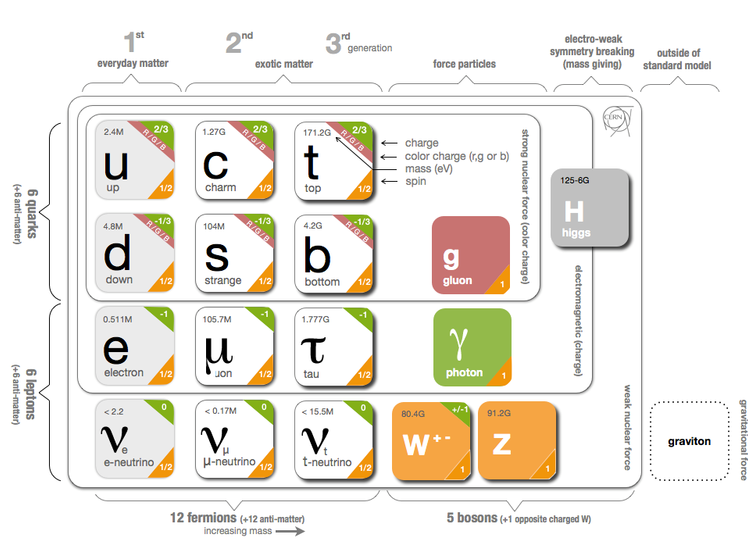
\includegraphics[width=1.3\linewidth]{SM.png}
		\caption[The Standard Model.]{The Standard Model contents, source \cite{SM}.\label{fig:SM}}
	\end{figure} 

	\begin{figure}[htb!]
		\centering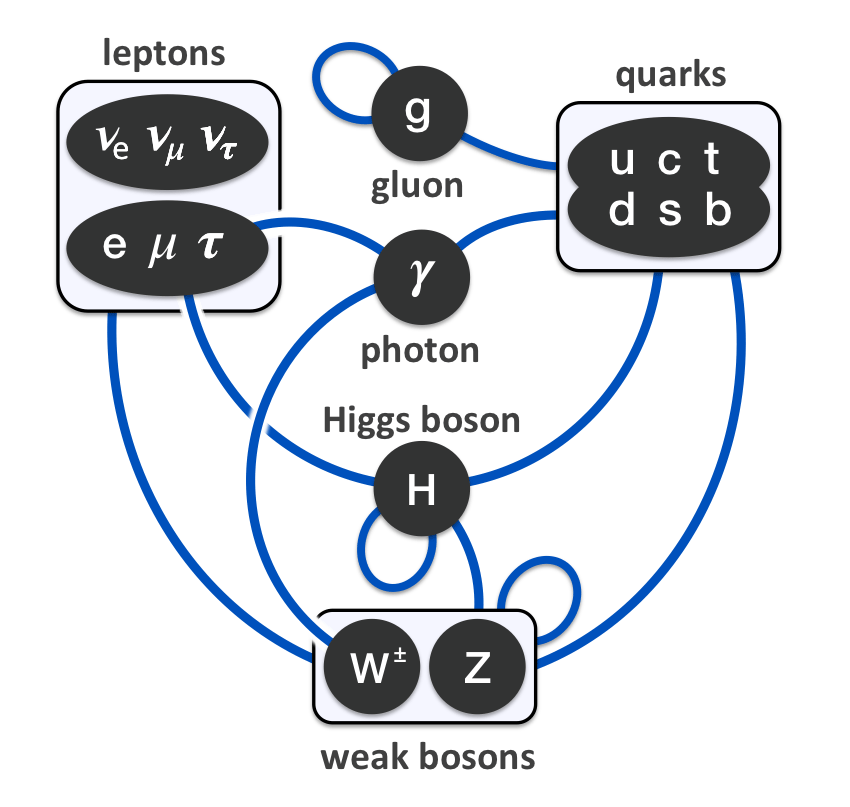
\includegraphics[width=0.5\linewidth]{Particle_interactions_SM.png}
		\caption[Particle interactions in the SM.]{The interaction between the particles in the Standard Model. Credit: Wikipedia.\label{fig:interactions_SM}}
	\end{figure} 


	\subsection{Gauge Bosons}
	\label{subsect:Theory-Bosons}
	From what we know of, there exists four fundamental forces. Three of these can be explained by the \acrshort{sm} through exchange of (gauge) bosons. That is why bosons also are called force-carrier particles. The three forces are the electromagnetic, strong and weak nuclear forces, where each force has its own connected boson(s). There are five different bosons that mediates these forces, and they all have integer spins. This means that they go with vector fields, along a direction.
	
		
	\subsubsection{Strong nuclear force} 
	\label{subsubsect:Theory-Strong_Force}
	The strong nuclear force is mediated by eight massless gluons (\textit{g}). They only affect the (r,g,b) color charged quarks, and come in combinations of color and anti-color charges. Since the six gluons carry a different variation of color and anti-color combinations, they come in an octet of colored states. The color assignments of these eight physical gluon variations can be written as:
	\[b\bar{g}, b\bar{r}, g\bar{b}, g\bar{r}, r\bar{b}, r\bar{g},\frac{1}{\sqrt{2}}(r\bar{r}-g\bar{g}), \frac{1}{\sqrt{6}}(r\bar{r}+g\bar{g}-2b\bar{b})\] 
	It is this strong interaction force that binds the quarks together to make e.g. protons and neutrons. The gluons can also self-interact with each other. This makes the interaction range of the strong nuclear force short, keeping the gluons within the nucleus. The exchange of gluons by interactions of colored particles is a mathematical model known as quantum chromodynamics (\acrshort{qcd}, sect.\ref{subsubsect:Theory-QCD}).
	
	
	\subsubsection{Electromagnetic force}
	\label{subsubsect:Theory-EM_Force}
	The electromagnetic force is mediated by the massless photon ($\gamma$). Photons have interact with electrically charged particles. Since the photon is massless and electrically neutral, it has an infinite range. The electromagnetic force is responsible for holding electrons in place around the nucleus, and is not as strong as the strong nuclear force. Electrically charged particles are either attracted to each other or repelled away for each other, dependent on if the charges of the particles have the same sign or not. The exchange of photons by interactions of charged particles is a mathematical model known as quantum electrodynamics (\acrshort{qed}, sect.\ref{subsubsect:Theory-QED}).
	
	
	\subsubsection{Weak nuclear force}
	\label{subsubsect:Theory-Weak_Force}
	The weak nuclear force is mediated by the $W^{\pm}$ and $Z^0$ bosons. There are two charged variants of the $W$ with charge $+e$ or $-e$. The $Z$ boson is electrically neutral. They er all massive which gives a short lifetime and short range. Because of the difference in charges, they act on different particles. The $W$ boson couples the electromagnetic interactions. The $W$ boson can decay to all flavors of quarks, except the top quark which is too massive, leptonic final states or hadronic final states. The weak interaction force can change the flavor of quarks. The exchange of $W$ and $Z$ bosons is explained with a more complex mathematical model that unifies both the weak and electromagnetic interactions, and it is known as electroweak theory (\acrshort{ewt}, sect.\ref{subsubsect:Theory-EWT}).
	
	
	\subsubsection{Gravitational force}
	\label{subsubsect:Theory-G_Force}
	The last force of nature is gravity. We have not yet found the hypothetical graviton (\textit{G}) particle which should carry the gravitational force. All the other forces seem to be well explained in the \acrshort{sm}, except for gravity. So the gravitational force is not included in the \acrshort{sm}. LIGO and Virgo discovered in 2015 gravitational waves from observing the merging of two black holes with $\sim$30 solar masses each \cite{GravitationalwaveDiscovery}, which might give insight into gravitons in the future. When looking at small objects (micro size), gravity does not seem to have any noticeable effect. But when we look at bigger objects of mass like humans or planets (macro size), then gravity has a much bigger effect and is well described by Einstein's General Theory of Relativity. Since gravity has more or less a negligible effect on particles energies so far probed in experiments, particle physicists do not have to take gravity into consideration.
	
	
	\subsection{Higgs Boson}
	\label{subsect:Theory-Higgs}
	The Higgs boson (H) is a "recently" discovered particle (2012) \cite{HiggsATLAS}\cite{HiggsCMS} theorized by Peter Higgs in 1964. This particle has intrinsic no spin, which makes it a scalar particle, and the only scalar particle discovered so far. It's electrically neutral and massive ($m_H\approx$125 GeV), and interacts with itself. Since it is so massive, the lifetime of the Higgs boson is very short and it's hard to detect directly. It can in principle decay to all massive \acrshort{sm} particles. The heavier particle, the stronger is the coupling to the Higgs.
	
	The discovery of the Higgs boson was a major contribution to the \acrshort{sm} since it can explain the origin of the masses of the other elementary particles. It also confirmed the existence of the Higgs (scalar) field, which gives the other elementary particles mass when they interact with this field. This field is thought to be everywhere in the universe with a non-zero vacuum expectation value. Here, Higgs bosons appear and disappear and interact with other particles in the field giving them their masses. The gluons and photons do not interact with this field, hence they are massless.
	
	
	\subsection{Fermions}
	\label{subsect:Theory-Fermions}
	The fermion group in the \acrshort{sm} consists of 12 elementary particles with half-integer spins. These particles are also known as matter-particles, since these particles are the building blocks of the matter in the universe. Each fermion has its own antiparticle. The antiparticles have the same mass as their particle partner, but has opposite electric charges and different quantum numbers. Fermions which acts as their own antiparticles are called Majorana particles.
	
	The 12 fermions can be split into two groups of six quarks and six leptons. The fermions can then be categorized into three generations, which goes from lighter and more stable to heavier and less stable. As seen in the \acrshort{sm} figure (\ref{fig:SM}), the first generation is called the "everyday matter". This is because most of the stable (baryonic) matter is made from the first generation particles. The reason for this is that the first generation particles do not decay. Second and third generation particles are only observed in high-energy environments. None of the neutrinos decay, but they oscillate and scatter, and they rarely interact with baryonic matter.
	
	
	\subsubsection{Quarks}
	\label{subsubsect:Theory-Quarks}
	The six quarks are up, down, charm, strange, top and bottom. A characteristic property for the quarks is that they all have color and electric charges, and they interact through the strong nuclear force. The colors charges are denoted red, green and blue and they all have an anti-color. Quarks cannot exist as free particles. As explained in section \ref{subsubsect:Theory-Strong_Force}, the quarks have a strong binding force between them since they are acted upon by the strong nuclear force. From this strong binding force, the quarks form particles called hadrons, like protons and neutrons. They are made up of either three quarks (baryons) or a quark and an anti-quark (mesons). A proton is made up of one down quark and two up quarks. The hadrons are color-neutral particles. Since quarks have electric charges, they also interact via the electromagnetic force and the weak nuclear force.
	
	
	\subsubsection{Leptons}
	\label{subsubsect:Theory-Leptons}
	The six leptons are electron ($e$), electron neutrino ($\nu_e$), muon ($\mu$), muon neutrino ($\nu_{\mu}$), tau ($\tau$) and tau neutrino ($\nu_{\tau}$). The electron, muon and tau leptons have electric charges and are influenced by electromagnetism. They all carry a $-1e$ electric charge, while their respective antiparticle having electric charge $+1e$. Every lepton carrying a lepton number, which is conserved in all known interactions. The leptons also interact weakly. Both leptons and antileptons have their respective lepton number +1 and -1, and each flavor has its own lepton flavor number with the same values as the lepton numbers. There are three generations where the three charged leptons are paired with their respective neutrino, and the masses of these three leptons increases with the generation. Only the electron (1st gen) is stable and doesn't decay, while the muon and tau leptons decay via the weak interaction.
	
%----

	\section{Neutrinos}
	\label{sect:Theory-Neutrino}
	The three neutrinos (electron, muon, tau) are a little more special than the other elementary particles. They are classified as leptons with half-integer spins, but they do not carry any charge and are thus neutral. They only interact via the weak nuclear force, making them very hard to observe since they go through almost everything without interacting much with anything. If the neutrinos are Majorana, they are the only Majorana fermions of the \acrshort{sm} since all the other fermions have an non-zero electric charge. By detection of neutrinos and antineutrinos, only left-handed neutrinos and right-handed antineutrinos are observed. From the weak nuclear force mediator particles, the $W^{\pm}$ bosons, we know that they only couple to left-handed particles and right-handed antiparticles. This means that interaction of the right-handed neutrinos is not covered in the \acrshort{sm}. Since mass terms couple both left- and right-handed states, the neutrinos are considered as massless in the \acrshort{sm}. Through the discovery of neutrino oscillations \cite{NeutrionOscillation}, we know that the neutrinos can change flavor meaning they cannot be massless. We know that they have to have mass since the neutrinos oscillate, but the mechanism behind the masses are not known. So, one type of neutrino can in fact change flavor to another type of neutrino when it travels over a large distance. Neutrino oscillation describes the difference between the neutrino flavor eigenstates and the neutrino mass eigenstates. This type of physics is not covered by the \acrshort{sm} and will be looked more into later in this thesis.
	
	
	\subsection{Neutrino Oscillations}
	\label{subsect:Theory-N_oscillations}
	From the \acrshort{sm} we know that for all interactions the lepton number is conserved for both the total and each lepton flavor separately. The lepton number is conserved when a $W^{\pm}$ boson decays into a lepton neutrino pair. We will in this thesis have a $W^{\pm}$ boson that decays into leptons
	
	The discovery of neutrino oscillations was done by two experiments. Namely the Super-Kamiokande Observatory\cite{superkamiokande} and the Sudbury Neutrino Observatories (\acrshort{sno})\cite{SNO} experiments. They got the Nobel Prize in physics in 2015 for their contributions by detecting solar neutrinos from the Sun \cite{gibney2015neutrino}. The Super-Kamiokande detected electron neutrinos using a big water \v{C}erenkov detector, but they got a too low electron neutrino flux than what was expected to be produced in the Sun. The \acrshort{sno} experiment showed that the atmospheric neutrinos and the neutrino flux from $\beta$-decay in the Sun had strong muon and tau components by using heavy water. Since only electron neutrinos are produced by nuclear fusion in the Sun, the neutrinos must have the ability to change their flavor when moving over large distances.
	
	The neutrino oscillation is a quantum-mechanical phenomenon, where the neutrino flavor (weak) eigenstates ($\nu_e, \nu_{\mu}, \nu_{\tau}$) can be related to the mass eigenstates ($\nu_1, \nu_{2}, \nu_{3}$) by an unitary transformation matrix $U$ as 
	\begin{equation*}
	\label{eq:Flavor_states}
		\begin{pmatrix}
		\nu_e \\ \nu_{\mu} \\ \nu_{\tau}
		\end{pmatrix} 
		= \begin{pmatrix}
		U_{e1} & U_{e2} & U_{e3} \\
		U_{\mu1} & U_{\mu2} & U_{\mu3} \\
		U_{\tau1} & U_{\tau2} & U_{\tau3}
		\end{pmatrix}
		\begin{pmatrix}
		\nu_1 \\ \nu_{2} \\ \nu_{3}
		\end{pmatrix}.
	\end{equation*} 
	The flavor eigenstates are linear combinations of the mass eigenstates. The $3\times3$ unitary matrix is the Pontecorvo-Maki-Nakagawa-Sakata (\acrshort{pmns}) matrix, and  it's expressed with three mixing (rotation) angles and a complex Dirac CP violation phase if the neutrinos are Dirac particles. The unitary of the \acrshort{pmns} matrix implies that $U^{-1}=U^{\dagger}\equiv(U^*)^T$ and $UU^{\dagger}=I$.
	
	If the neutrino mass eigenstates are not the same, we get neutrino oscillations from the phase differences in components of the wavefunction. Since we already know that the neutrinos change flavor from the discovery of neutrino oscillations, we know that the neutrinos need some mass, differing by flavor, to being able to change flavor. That is why the neutrinos need non-zero masses and not equal to each other for neutrino oscillations to be true. From experimental measurements, like long baseline accelerators, for the neutrino masses there is only found upper limits to the masses. The best upper limits on the neutrino masses was found to be
	\begin{equation}
	\label{eq:Neutrino_mass_limit}
		\sum_{i=1}^{3}m_{\nu_i}\lesssim 1.1 \text{eV}
	\end{equation}
	by the Karlsruhe Tritium Neutrino (\acrshort{katrin})\cite{KATRIN} experiment in Germany.
	The reason why the neutrino masses seems to be so much smaller than the other fundamental particles is not known.
	
%----	
	
	\section{Symmetries}
	\label{sect:Theory-Symmetry}
	Particle dynamics are heavily influenced by symmetries and laws of conservation. From classical Newtonian physics, we know that energy (\textit{E}), three-momentum ($\vec{p}$) and total angular momentum (\textit{J}) are conserved quantities. This is also the case in the \acrshort{sm}. A quantity that is not conserved is the (rest) mass (\textit{m}). This is something we know according to Einstein's Special Relativity. This enables production of heavier particles than the colliding particles.
	
	Another fundamental symmetry of physical laws is the CPT theorem. The CPT theorem is one of the results concluded by quantum field theory (\acrshort{qft}), and states that all physical processes are symmetric under CPT-transformation \cite{CPT}. C is charge conjugation, where every particle can be replaced by its antiparticle. P is parity reflection, where everything in the universe is mirrored along the three physical axes. T is time reversal, where the direction of time is reversed in the sense of looking at the local properties of the \acrshort{sm}. The combination of these three symmetries is predicted by the \acrshort{sm} to be a symmetry, while each symmetry alone is only a near-symmetry. The CPT symmetry explains why particles and antiparticles have identical masses, magnetic moments, etc. The CPT is also thought to be an exact symmetry in the Universe. Only the weak interactions of quarks and leptons seems to violate the C-, P-, T- and CP-symmetries out of the three fundamental forces explained by the \acrshort{sm}.
	
	A topic to be further discussed later is gauge theory (sect. \ref{subsect:Theory-Qauge}). From the connected gauge symmetry in the \acrshort{sm}, we get a conservation of certain quantum numbers during the different interactions with the fundamental forces based on the $SU(3)\times SU(2)\times U(1)$ group. The quantities that are conserved are: the color charge for the strong nuclear interaction ($SU(3)$), the electric charge for electromagnetic interactions ($U(1)$) and the weak isospin for the weak nuclear interaction ($SU(2)$).
	
	Other important conservation laws are the conservation of baryon number, $B$, and lepton number, $L_x$, in an interaction. $x$ is the lepton flavor. The only case where the lepton number is not conserved is for neutrino oscillation. As we have explained earlier, neutrinos can change flavor when traveling large distances. But, this is not something we have to be concerned about in our case since we look at particles in particle detectors over short distance. This distance is not big enough for neutrino oscillations to occur.
	
%----	

	\section{Quantum Field Theory}
	\label{sect:Theory-QFT}
	The Standard Model is based on the framework of quantum field theory (\acrshort{qft}). This is a theory that combines quantum mechanics, special relativity and field theory. In other words, quantum field theory tries to explain the little things in the universe, like the elementary particles, that move very fast, close to or with light speed $c$. This also means that every elementary particle has its own associated field. These fields can then be explained in terms of the Lagrangian density, $\mathcal{L}$, to explain the dynamics and kinematics of the fields.
	
	The combination of quantum mechanics and special relativity does give some problems. The most important equation in quantum mechanics is the Schrödinger equation, and it's not Lorentz invariant. The problem with this is that Schrödinger's equation is not the same for two observers in different reference frames. Other problems this leads to is that we get violation of causality, negative energy states and there is no possibility for new particle creations. The good thing is that these problems can be fixed by exchanging the Schrödinger equation (see Notation and Conventions) by the Dirac equation \cite{mandl2010quantum}\cite{Bellac1991QuantumAS} for $\frac{1}{2}$-spin particles and the Klein-Gordon equation \cite{mandl2010quantum}\cite{Bellac1991QuantumAS} for scalar particles. With the Dirac and Klein-Gordon fields, this leads to specific (gauge) theories for different particles and associated interactions, which we have briefly mentioned earlier and will explain more soon.
	
	
	\subsection{The Lagrangian}
	\label{subsect:Theory-Lagrangian}
	For more simple classical mechanics cases the Lagrangian is just given as the difference between the kinetic energy, $K$, and the potential energy, $V$, $L=K-V$. This is also a baseline for the \acrshort{qft}.
	By using the Lagrangian of a system with a set of generalized coordinates $q_i$ and their time derivatives $\dot{q}_i$, we can find the equation of motion that describes the system by using the Euler-Lagrange equation,
	\begin{equation}
	\label{eq:Euler-Lagrange}
		\frac{d}{dt}\left(\frac{\partial L}{\partial \dot{q}_i}\right) - \frac{\partial L}{\partial q_i}=0.
	\end{equation} 
	
	A difference for \acrshort{qft} is that instead of kinetic and potential energies, or the generalized coordinates, we use fields with four space-time coordinates. This changes the Lagrangian $L$ to the Lagrangian density $\mathcal{L}$ as a continuous system. This is a function of the fields, $\phi_i(t,x,y,z)$, and their derivatives, $\partial_{\mu}\phi_i(t,x,y,z)$. Since $L$ is the spatial integral over $\mathcal{L}$, 
	\begin{equation}
	\label{eq:L_int}
		L=\int\mathcal{L}d^3\textbf{x},
	\end{equation} 
	and using the principle of least action \cite{least_action}, the new Euler-Lagrange equation becomes 
	\begin{equation}
	\label{eq:Euler-Lagrange-QFT}
		\partial_{\mu}\left(\frac{\partial \mathcal{L}}{\partial (\partial_{\mu}\phi_i)}\right) - \frac{\partial \mathcal{L}}{\partial \phi_i}=0.
	\end{equation}
	For simplicity we will just denote the Lagrangian density the Lagrangian from now on. From this new Euler-Lagrange equation, we can derive both the free-particle Dirac and the Klein-Gordon equations by imposing the Lagrangian with a free fermion field\footnote{Relativistic spin-half fields, Chapter 17.2.2 in \citet{thomson2013modern}} and free theory\footnote{Relativistic scalar fields, Chapter 17.2.2 in \citet{thomson2013modern}} respectively. The Lagrangian for the spin-half (spinor) field, $\psi$, is
	\begin{equation}
	\label{eq:L_spinor}
		\mathcal{L}_D=i\bar{\psi}\gamma^{\mu}\partial_{\mu}\psi-m\bar{\psi}\psi,
	\end{equation}
	and the Lagrangian for the non-interacting scalar field, $\phi$, is
	\begin{equation}
	\label{eq:L_scalar}
		\mathcal{L}_S=\frac{1}{2}(\partial_{\mu}\phi)(\partial^{\mu}\phi)-\frac{1}{2}m^2\phi^2.
	\end{equation}
	Both of these two equations for the Lagrangian contain a kinematic term and a mass term. 
	
	With perturbation theory in quantum mechanics, the Lagrangian can also be used to describe the behavior and interaction of elementary particles with Feynman diagrams for simpler visualization of usually complex particle interactions.
	
	
	\subsection{Qauge Theories}
	\label{subsect:Theory-Qauge}
	From the new Lagrangian we now know that we need some new theory to explain the interactions between the elementary particles, since these interactions vary depending on the particles and associated interactions involved. In this theory we need to require that the Lagrangian stays invariant under local transformations using symmetry or gauge groups. In special relativity, this global symmetry group is called the Poincaré group which includes spacetime symmetries. 
	
	To describe the \acrshort{sm} we need an internal gauge invariant symmetry that represents the different elementary interactions and is independent of spacetime coordinates. This is the local $SU(3)\times SU(2)\times U(1)$ gauge symmetry group. Here each special unitary group with degree $n$ (the number in the parenthesis) is connected to its own gauge theory and the three elementary interactions in the \acrshort{sm}, and $n$ is a $n$-dimensional space. If a symmetry group is commutative, meaning that regardless of what the order of the elements are applied the result will be the same, then it is called an Abelian group. If the group is non-commutative, it is then a non-Abelian gauge theory which implies the existence of gauge boson self-interaction.
	
	
	\subsubsection{Quantum chromodynamics (QCD)}
	\label{subsubsect:Theory-QCD}
	The gauge theory that defines the strong interaction between the quarks and (eight) gluons (color charged particles) is the quantum chromodynamics sector \cite{QCD}. The \acrshort{qcd} conserves the separately conserved color charges red, green and blue, and thus works in a three dimensional color space. Another quantity which is conserved in \acrshort{qcd} is parity. This comes from that the \acrshort{qcd} interaction Hamiltonian is invariant under parity transformations (sect. 11.2.2 in \citet{thomson2013modern}). The antiquarks carry the opposite color charge to the quarks of red, green and blue. The color states consists of color isospin and color hypercharge. It also ensures invariance under the local gauge transformation. The gauge symmetry group for this sector is $SU(3)_C$ and is represented by $3\times3$ matrices, where the $C$ stands for the conserved color. This symmetry group does not commute and is a non-Abelian gauge theory, or more precise it is a Yang-Mills gauge theory \cite{Yang-Mills}. By using this gauge theory, we can derive a new invariant Lagrangian which does not have a mass term for the gluons:
	\begin{equation}
	\label{eq:L_QCD}
		\mathcal{L}_{QCD}=\bar{\psi}(i\gamma^{\mu}\partial_{\mu}-m)\psi -\frac{1}{2}g_s\bar{\psi}\gamma^{\mu}\lambda_a\psi G_{\mu}^a -\frac{1}{4}G_{\mu\nu}^aG_a^{\mu\nu}
	\end{equation}
	$\psi$ is a fermion (quark) field, $g_s$ is a coupling constant of the strong interaction, $\gamma^{\mu}$ are Dirac matrices, $a=1,...,8$ are the eight gluons, $\lambda_a$ is one of the eight Gell-Mann matrices and $G_{\mu\nu}^a$ is a gauge invariant gluon field strength tensor. The last term of the Lagrangian in equation \ref{eq:L_QCD} implies that the gluons should be massless and can self-interact. 
	
	In Figure \ref{fig:QCD} we see the \acrshort{qcd} vertices for quark and gluon interactions (and self-interacting gluons).
	
	\begin{figure}[htbp!]
		\centering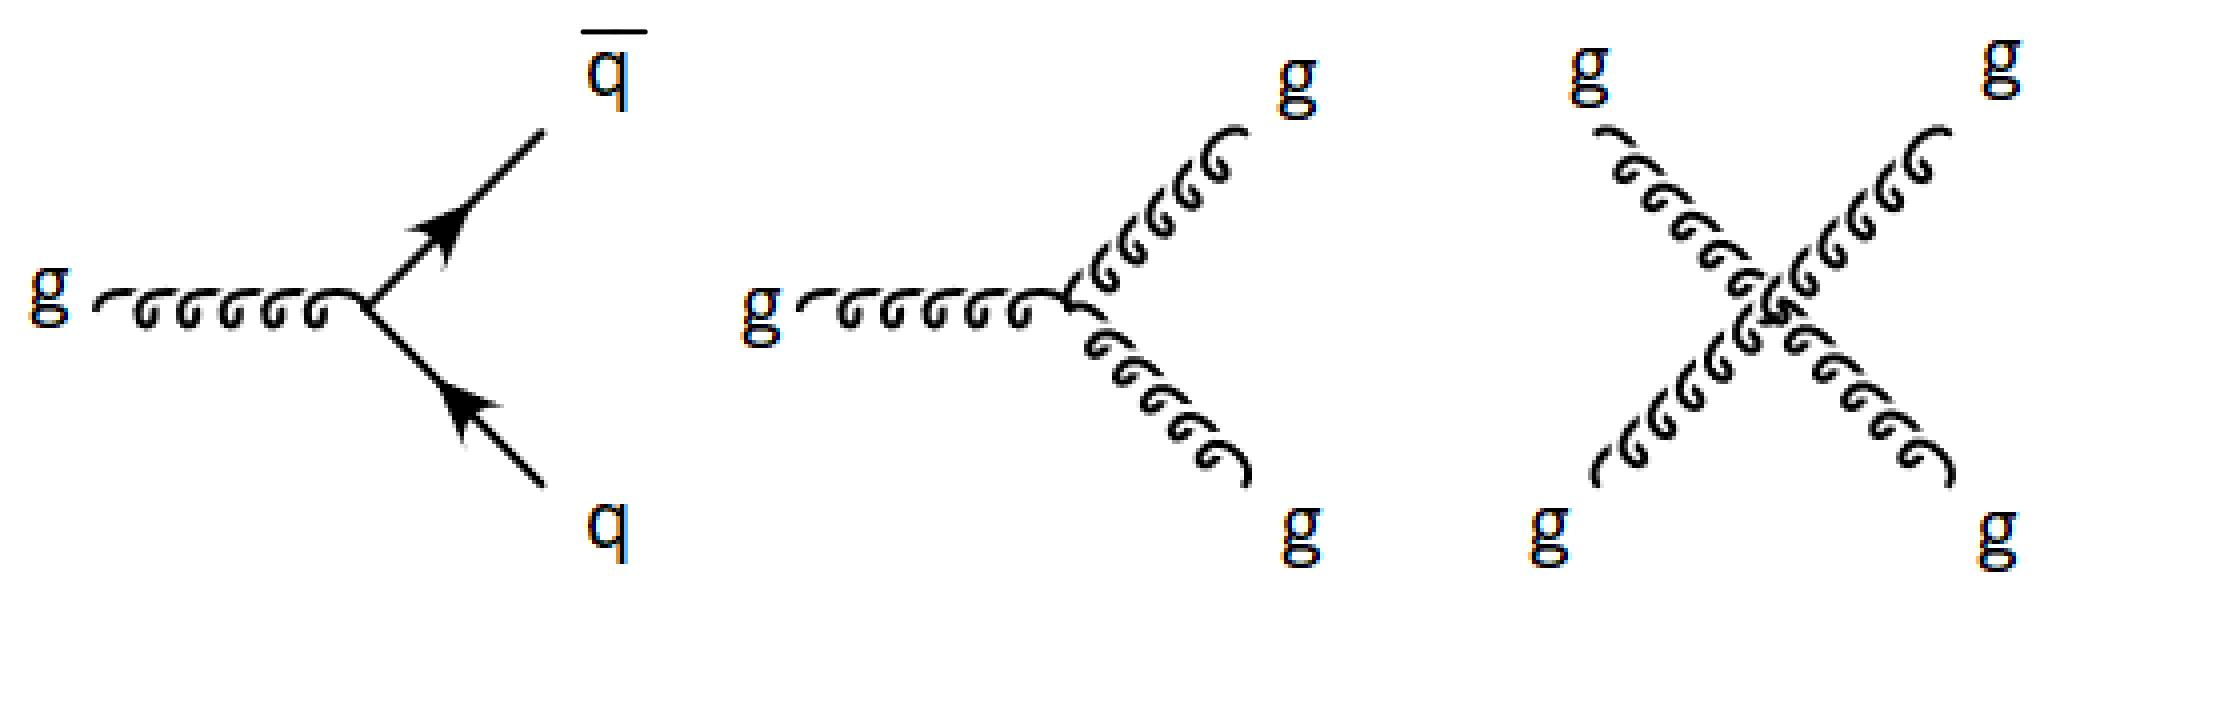
\includegraphics[width=0.8\linewidth]{QCD.png}
		\caption[\acrshort{qcd} vertex Feynman diagrams.]{Here we see Feynman diagrams of the basic \acrshort{qcd} vertices. From left to right we see, the coupling of gluon fields (g) interaction with quark fields (q), a triple gluon vertex and a quartic gluon vertex. Source Fig. 10.1 in \citet{thomson2013modern}. \label{fig:QCD}}
	\end{figure}
	
	
	\subsubsection{Quantum electrodynamics (QED)}
	\label{subsubsect:Theory-QED}
	The gauge theory that defines the electromagnetic interaction for the electrically charged particles and photons is the quantum electrodynamics sector \cite{QED}. The \acrshort{qed} conserves the electric charge of the particles. Like in \acrshort{qcd}, parity is conserved in \acrshort{qed} (sect. 11.2.2 in \citet{thomson2013modern}). The gauge symmetry group for \acrshort{qed} is $U(1)$ which is an Abelian group. By starting with a free fermion field for the Lagrangian (eq.\ref{eq:L_spinor}, invariant under \textit{global} $U(1)$ transformation) and require invariance under a local phase transformation, leads to a Lagrangian with a Lorentz-invariant description where there is an electromagnetic interaction between fermions and the gauge field of the massless photon:
	\begin{equation}
	\label{eq:L_QED}
		\mathcal{L}_{QED}=\bar{\psi}(i\gamma^{\mu}\partial_{\mu}-m_e)\psi +e\bar{\psi}\gamma^{\mu}\psi A_{\mu} -\frac{1}{4}F_{\mu\nu}F^{\mu\nu}.
	\end{equation}
	$\psi$ is the field of the spin half particles, $e$ is a coupling constant of the electromagnetic interaction, $\gamma^{\mu}$ are Dirac matrices, $A_{\mu}$ is a covariant four-potential (gauge field), and $F_{\mu\nu}$ is the electromagnetic field strength tensor.
	
	From the Lagrangian in equation \ref{eq:L_QED}, we can construct the Feynman diagram of a \acrshort{qed} interaction vertex between a single photon and two spin-half fermions, seen in Figure \ref{fig:QED}.
	\begin{figure}[htbp!]
		\centering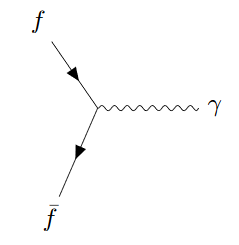
\includegraphics[width=0.3\linewidth]{QED.png}
		\caption[\acrshort{qed} vertex Feynman diagram.]{A Feynman diagram of the basic \acrshort{qed} vertex for the interaction between fermions (f) and a massless photon ($\gamma$). Source Fig. 5.6 (and 10.10a) in \citet{thomson2013modern}. \label{fig:QED}}
	\end{figure}
	
	
	\subsubsection{Electroweak theory (EWT)}
	\label{subsubsect:Theory-EWT}
	The gauge theory which defines the weak interaction for the 3rd component of isospin particles and the $W$ and $Z$ bosons/fields is the unified theory known as electroweak theory (\acrshort{ewt}) \cite{EWT} or Glashow-Weinberg-Salam (\acrshort{qws}) theory. This theory (from the 1960's) earned the three contributors Glashow\cite{glashow1961partial}, Weinberg\cite{weinberg1967model} and Salam\cite{salam1968n} the Nobel Prize in Physics in 1979 \cite{NobelPrizeEWT}\cite{salam1979nobel}.
	
	Unlike \acrshort{qcd} and \acrshort{qed}, it is found experimentally that parity is not conserved in the weak interaction (sect. 11.2.3 in \citet{thomson2013modern}). This parity-violation makes the weak interaction treat left-handed and right-handed particles differently. The charge-current weak interaction is invariant under $SU(2)$ local phase transformations and includes weak isospin. The cross-section of $W$-pairs produced at higher energies, violates quantum mechanical unitarity such that particle probability is no longer conserved. This is solved because the couplings of the $\gamma$ (\acrshort{qed}), $W^{\pm}$ and $Z$ \acrshort{ewt} are related to each other in the unified electroweak model.
	
	 In the \acrshort{ewt} theory fermions exists as left- and right-handed chirality states, while $W$-bosons only couple to left-handed fermions. The \acrshort{ewt} conserves the flavor charge and weak isospin of the particles. It is the weak isospin quantum number that accounts for the $W$-boson coupling, since left-handed fermions have half-isospin and appears as isospin doublets while right-handed fermions appear as isospin singlets. Something to take notice of here is that, the weakly interacting quarks are superpositions of the mass eigenstates while the strongly interacting quarks are mass eigenstates.
	
	The electroweak theory is based on the $SU(2)_L\times U(1)_Y$ symmetry group, where $L$ is left-handed interaction and $Y$ is the weak hypercharge expressed by the electric charge $Q$ and the third component of the weak isospin $I_3$, $Y=2(Q-I_3)$. This new $U(1)_Y$ local gauge symmetry is used instead of that in \acrshort{qed}, where the charge now has been replaced by the weak hypercharge. Each gauge invariant transformation in this theory, introduce new gauge fields which as linear combinations corresponds to the photon and the $W$ and $Z$ bosons of the weak interaction. With these new gauge fields, we can derive yet another new preliminary (electroweak) Lagrangian that is associated with the \acrshort{ewt} theory: 
	\begin{align}
	\label{eq:L_EWT}
		\mathcal{L}_{EWT}=& \bar{\psi}_L\gamma^{\mu}
		\left[i\partial_{\mu}-\frac{1}{2}g\boldsymbol{\sigma}\textbf{W}_{\mu}-\frac{1}{2}g^{\prime}YB_{\mu}\right]
		\psi_L +\bar{\psi}_R\gamma^{\mu}\left[i\partial_{\mu}-\frac{1}{2}g^{\prime}YB_{\mu}\right]\psi_R \nonumber\\ 
		&-\frac{1}{4}B_{\mu\nu}B^{\mu\nu} -\frac{1}{4}\textbf{W}_{\mu\nu}\textbf{W}^{\mu\nu}
	\end{align}
	$\psi_{L,R}$ are the fields for left- and right-handed fields respectively, $g$ and $g^{\prime}$ are coupling constants related to the elementary charge, $\gamma^{\mu}$ are the Dirac matrices, $\boldsymbol{\sigma}$ are the Pauli matrices, $B_{\mu}$ is a field strength tensor for the weak hypercharge gauge field for $U(1)_Y$, $\textbf{W}_{\mu\nu}$ is a field strength tensor for the three weak isospin gauge fields for $SU(2)_L$. 
	
	The \acrshort{ewt} gauge symmetry group is non-Abelian. In Figure \ref{fig:EWT-f} and \ref{fig:EWT-W} we see Feynman diagrams of the electroweak interaction vertices including fermions and gauge boson self-interactions. The photon and the $Z$-boson couple with both left- and right-handed fermions, while the $W$-bosons do not.
	
	\begin{figure}[htbp!]
		\centering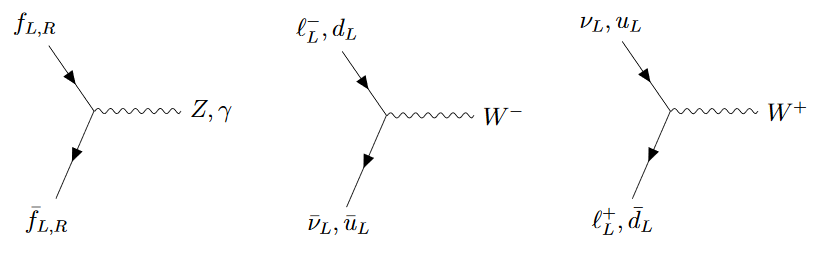
\includegraphics[width=0.9\linewidth]{EWT-f.png}
		\caption[EWT fermion vertex Feynman diagrams.]{Here we see Feynman diagrams of the electroweak interaction vertices that includes fermions. \label{fig:EWT-f}}
	\end{figure}
	\begin{figure}[htbp!]
		\centering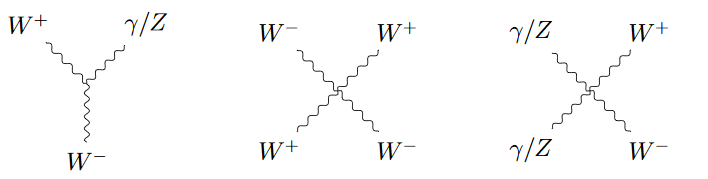
\includegraphics[width=0.9\linewidth]{EWT-W.png}
		\caption[EWT gauge boson vertx Feynman diagram.]{Here we see Feynman diagrams of the electroweak interaction vertices for gauge boson self-interaction. \label{fig:EWT-W}}
	\end{figure}

	
	By introducing the \acrshort{beh} mechanism we get, in addition to the coupling in Figure \ref{fig:EWT-f} and \ref{fig:EWT-W}, couplings between the Higgs boson and the massive gauge boson as well as Higgs self-interaction. These couplings can be seen in Figure \ref{fig:EWT-H}.
	\begin{figure}[htbp!]
		\hspace*{-0.5cm}
		\centering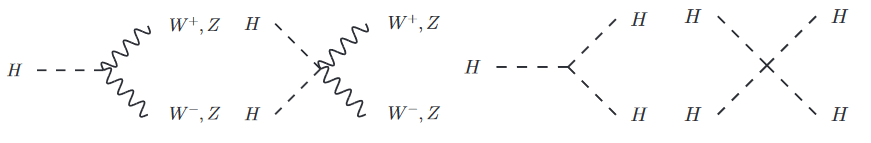
\includegraphics[width=1.1\linewidth]{EWT-H.png}
		\caption[Higgs-bosons coupling Feynman diagrams.]{Here we see Feynman diagrams of the couplings between the Higgs boson and the massive gauge bosons and Higgs self-interaction. \label{fig:EWT-H}}
	\end{figure}

	\textbf{Fermion masses:}
	The Higgs mechanism can also be used to give masses to the fermions. The Higgs isospin doublet has a lower and an upper element. The lower element is used to give masses to down-type quarks and charged leptons, while the masses of the up-type quarks are constructed from the conjugate doublet. The gauge invariant mass terms of the Dirac fermions are then described as 
	\begin{equation}
	\label{eq:Dirac_fermion_masses}
		m_f=\frac{g_fv}{\sqrt{2}},
	\end{equation}
	where $g_f$ is the Yukawa coupling constant of the fermions to the Higgs field, as shown in Figure \ref{fig:Yukawa}. 
	
	\begin{figure}[htbp!]
		\centering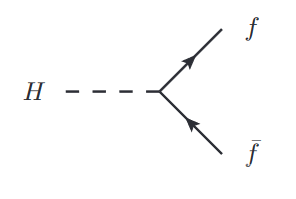
\includegraphics[width=0.3\linewidth]{Yukawa-coupling.png}
		\caption[Higgs-fermions coupling diagram.]{Here we see Feynman diagrams of the coupling between the Higgs boson and fermions. \label{fig:Yukawa}}
	\end{figure}
	
	
	\subsubsection{Full EWT Lagrangian}
	\label{subsubsect:Theory-Full_L}
	The complete Lagrangian for the \acrshort{ewt} is given by:
	\begin{align}
	\label{eq:Full_EWT}
		\mathcal{L}_{EWT}=& \overline{\psi}_L\gamma^{\mu}
		\left[i\partial_{\mu}-\frac{1}{2}g\boldsymbol{\sigma}\textbf{W}_{\mu}-\frac{1}{2}g^{\prime}YB_{\mu}\right]
		\psi_L +\overline{\psi}_R\gamma^{\mu}\left[i\partial_{\mu}-\frac{1}{2}g^{\prime}YB_{\mu}\right]\psi_R \nonumber\\ 
		&-\frac{1}{4}B_{\mu\nu}B^{\mu\nu} -\frac{1}{4}\textbf{W}_{\mu\nu}\textbf{W}^{\mu\nu} +\bigg|\left(i\partial_{\mu}-\frac{1}{2}g\boldsymbol{\sigma}\textbf{W}_{\mu}-\frac{1}{2}g^{\prime}YB_{\mu}\right)\phi\bigg|^2 \nonumber\\
		&-V(\phi) -(g_f\overline{\psi}_L\phi\psi_R +G_f^{\prime}\overline{\psi}_L\phi_c\psi_R+h.c.)
	\end{align}
	The first line is the couplings between the fermions and the gauge fields and kinetic terms for the fermion fields. The second line is the kinetic terms for the gauge fields and the Higgs field, the couplings between the gauge field and the Higgs field, and the couplings between the gauge fields. The third line contains the scalar potential, the Yukawa coupling terms and the fermion mass terms, and $h.c$ stands for the corresponding Hermitian conjugate.
	
	
%-------------------------------------------------------------------------

	\chapter{Neutrinos Beyond the Standard Model}
	\label{chap:Theory-Beyond_SM} 
	The \acrshort{sm} explains most of the physics we measure in  experiments. The \acrshort{sm} has several free parameters which are chosen to match observations. Nevertheless, the \acrshort{sm} does not explain everything. For theorists the ultimate goal is to construct a Theory of everything, which explain all the physical phenomena in a unified way (including also gravity). Particle physicists try to address the shortcomings of the \acrshort{sm} by extending it and construct more complete models which can explain e.g. gravity or the masses of the neutrinos.
	
	A major problem in today's particle physics is that the \acrshort{sm} can only explain about 5\% of the total energy density of the Universe. This 5\% of the matter in the Universe is called baryonic matter, while the rest is something yet unknown. One theory is that about 25\% is something called dark matter, that acts as matter, but we can't see it, and has a gravitational pull in the Universe. The remaining 70\% is then thought to be dark energy, which has a pushing affect on the galaxies in the Universe making it expanding faster and faster with time. A dark matter candidate is neutrinos. We will not go into the dark matter aspect, but look closer at neutrinos and the neutrino masses.

	From the discovery of neutrino oscillations, we know from observations and experiments, that the neutrinos need to have mass since they have the ability to change flavor over very large distances. Why the neutrinos have mass and what gives them mass, on the other hand, are not explained in the \acrshort{sm}. The only place in the \acrshort{sm} that allows CP-violation, is in the weak interaction domain where left-handed neutrinos are affected through neutrino mixing. Since it is not observed right-handed neutrinos nor left-handed antineutrinos, C- and P-symmetry should be violated. It has not yet been observed if CP-violations occur in neutrino oscillations, since neutrinos seem to uphold the CP-symmetry with the existence of right-handed antineutrinos. This means that some new physics is required to explain this breaking of CP-violation.
	
	For the neutrinos to acquire mass, we have to go beyond the \acrshort{sm} neutrino knowledge, and introduce some new theories. We will look more into the neutrino masses and the model for this thesis in this chapter.
	
%----
	
	\section{Neutrino Masses}
	\label{sect:Theory-Neutrino_beyond} 
	According to the \acrshort{sm}, neutrinos do not have mass because only left-handed (\acrshort{lh}) neutrinos are covered by the \acrshort{sm} and thus, right-handed (\acrshort{rh}) neutrinos are not involved in any of the fundamental interactions and have not yet been observed. As mentioned earlier, we know from observations and experiments of neutrino oscillations that neutrinos have a tiny, but non-zero mass. to being able to change flavor when moving over large distances. The neutrino masses are something we need to look more into.
	

	\subsection{Dirac Neutrinos}
	\label{subsect:Theory-Dirac_n}
	Dirac particles are particles which can be distinctively separated from its antiparticle. The Dirac field is described by a four-component Dirac spinor $\psi$ and can be divided into a left-handed $\psi_L$ and a right-handed $\psi_R$ part as two component Weyl spinors:
	\begin{equation}
	\label{eq:Dirac_spinors}
		\psi=
		\begin{pmatrix}
		\psi_L \\ \psi_R 
		\end{pmatrix}.
	\end{equation}
	The left-handed neutrinos in the \acrshort{sm} are described by this left-handed Weyl field. Since the Dirac mass term require both left- and right-handed fields in the \acrshort{sm}, there is no Dirac mass term for the neutrinos.
	
	If we assume neutrinos as Dirac particles, the neutrino mass is added similarly to the up-type quarks as the conjugate Higgs doublet. The gauge invariant Dirac neutrino mass term after spontaneous symmetry breaking becomes 
	\begin{equation}
	\label{eq:Dirac_neutrino}
		\mathcal{L}_D=-m_{\nu}(\overline{\nu_R}\nu_L + \overline{\nu_L}\nu_R),
	\end{equation}
	with the neutrino mass still determined by the Yukawa coupling constant as for Dirac fermions (eq. \ref{eq:Dirac_fermion_masses}):
	\begin{equation}
	\label{eq:Dirac_neutrino_mass}
		m_{\nu}=\frac{g_{\nu}v}{\sqrt{2}}
	\end{equation}
	
	The neutrino masses have been found to be several orders of magnitude smaller than the charged lepton masses. This leads to a Yukawa coupling constant $g_{\nu}\leq 10^{-12}$ for neutrino masses that are less than 1.1 eV (sect. \ref{subsect:Theory-N_oscillations}). There are no reasons why the Yukawa constants should be so small, which gives reason to believe that there must be some other mechanism giving neutrinos their masses. The right-handed neutrino in the \acrshort{sm} would be sterile and only interact with the Higgs boson.

		
	\subsection{Majorana Neutrinos}
	\label{subsect:Theory-Majorana_n}
	Another option for the neutrinos, is that they can be Majorana neutrinos. This means that they can be their own antiparticles. The result of this would mean that the lepton number no longer is conserved, which it is in the \acrshort{sm}. To not break the gauge invariance of the \acrshort{sm} when adding the fields for \acrshort{rh} neutrinos and \acrshort{lh} antineutrinos in the Lagrangian, the \acrshort{lh} antineutrinos appear as the CP conjugate field of the \acrshort{rh} neutrino\cite{thomson2013modern} defined by
	\begin{equation}
	\label{eq:LH_antin_CP}
		\psi^c_L = \hat{C}\hat{P}\psi= C\overline{\psi}_R^T,
	\end{equation}
	where $C$ is the charge conjugation matrix. 
	
	For a Majorana neutrino we have $\psi^c=\psi$, which means that the neutrino field can be expressed with a Majorana spinor
	\begin{equation}
	\label{eq:Majorana_spinors}
		\psi_{\nu}=
		\begin{pmatrix}
		\overline{\nu_R^c} \\ \nu_R 
		\end{pmatrix}
	\end{equation}
	for \acrshort{lh} and \acrshort{rh} neutrino fields and the CP conjugate of the \acrshort{rh} field (or the \acrshort{lh} antineutrino) $\overline{\nu_R^c}$. The local gauge invariant Majorana neutrino mass term, with Majorana mass $M$, becomes
	\begin{equation}
	\label{eq:Majorana_neutrino}
		\mathcal{L}_M=-\frac{1}{2}M(\overline{\nu^c_R}\nu_R + \overline{\nu_R}\nu_R^c). 
	\end{equation}
	
	This means that the Majorana mass term is not constrained by gauge symmetry and can be arbitrary large. The global baryon number minus the lepton number ($B-L$) symmetry of the \acrshort{sm} would be broken if the neutrino is a Majorana neutrino. From observations of the asymmetry between matter and antimatter in the Universe, it actually looks like the baryon number is not conserved. 
	
	A generic Majorana mass matrix, $\mathcal{M}$, with three neutrinos can also be expressed as 
	\begin{equation}
	\label{eq:MajoranaMatrix}
		\mathcal{M}=\begin{pmatrix}
			M_{L} & m_D \\ m_D^T & M_R
		\end{pmatrix}
	\end{equation}
	$m_D$ is the mass for a Dirac neutrino, $M_L$ is the Majorana mass for a \acrshort{lh} neutrino ($\nu_L$) and $M_R$ is the Majorana mass for a \acrshort{rh} neutrino ($\nu_R$).
	
	
	\subsection{Pseudo-Dirac Neutrinos}
	\label{subsect:Theory-PseudoDiracN}
	A pseudo-Dirac neutrino\cite{chang2000pseudo}\cite{balaji2002revisiting} mass matrix is similar to the Majorana mass matrix in equation \ref{eq:MajoranaMatrix}, except that the $M_L$ and $M_R$ masses are the lepton number violating Majorana masses of light neutrinos\footnote{A \acrshort{rh} neutrino is also called a sterile neutrino, $\nu_s$.}. When the Dirac mass is $m_D>>M_L,M_R$, we get a pseudo-Dirac mass matrix where the eigenvalues of the resulting mass eigenstates are close to each other. This means that the two light neutrinos can form a Dirac-like/pseudo-Dirac neutrino.
	
	
	\subsection{The Seesaw Mechanism}
	\label{subsect:Theory-Seesaw}
	One of many theories for the light masses of the neutrinos is to add \acrshort{rh} neutrinos that couple to the \acrshort{lh} neutrinos. However, this would lead to a disparity problem regarding mass scale. To solve this, a seesaw mechanism is introduced where the observed (light Dirac) \acrshort{lh} neutrinos couple with very heavy (sterile) Majorana \acrshort{rh} neutrinos. This would explain the small masses of the observed \acrshort{sm} left-handed neutrinos and the absence of observation of \acrshort{rh} neutrinos. The problem is that the mass scale of the \acrshort{rh} neutrinos is unknown, since the masses of the Dirac neutrinos are still uncertain. So they could be somewhere between a few keV, and possibly be light dark matter particle candidates, or have higher masses near the unification energy (GUT scale), where the electromagnetic, weak and strong forces have equal strength.
	
	
	\subsubsection{Type-I seesaw mechanism}
	\label{subsubsect:Theory-Type-I seesaw}
	There are several varieties of the seesaw mechanism which extends the \acrshort{sm}, but the simplest one is the \textbf{Type-I seesaw mechanism}\cite{mohapatra2005seesaw}. This involves the mix of \acrshort{lh} Dirac neutrinos and \acrshort{rh} Majorana neutrinos. In this theory, a right-handed neutrino is added for each of the \acrshort{sm} \acrshort{lh} neutrinos, in total three. When involving neutrinos as Majorana, we get that $\overline{\nu_L}\nu_R$ is equivalent to $\overline{\nu^c_R}\nu_L^c$. The Lagrangian after the spontaneous electroweak symmetry breaking with both the Dirac and Majorana mass terms becomes:
	\begin{equation}
	\label{eq:L_Dirac_Majorana}
		\mathcal{L}_{DM}=-\frac{1}{2}\left(m_{D}\overline{\nu_L}\nu_R + m_{D}\overline{\nu_R^c}\nu_L^c+M\overline{\nu^c_R}\nu_R\right) + h.c.
	\end{equation}
	$m_D$ is the Dirac mass and $M$ is the Majorana mass. This seesaw mechanism is characterized by $M_L<<m_D<<M_{(R)}$. This equation can also be written in terms of a $2\times2$ mass matrix ($\mathcal{M}$) for the neutrinos:
	\begin{equation}
	\label{eq:L_Dirac_Majorana_matrix}
		\mathcal{L}_{DM}=-\frac{1}{2}(\overline{\nu_L}\overline{\nu^c_R}) \begin{pmatrix}
		0 & m_D \\ m_D & M
		\end{pmatrix}
		\begin{pmatrix}
		\nu_L^c \\ \nu_R
		\end{pmatrix}
		+ h.c.
	\end{equation}
	By looking at the eigenvalues ($\lambda$) of the mass matrix $\mathcal{M}$ we get the physical masses of the neutrinos (in this model) as (sect.17.8.1 in \citet{thomson2013modern})
	\begin{equation}
	\label{eq:Neutrino_mass_phys}
		m_{\pm}=\lambda_{\pm}=\frac{M\pm M\sqrt{1+4m_D^2/M^2}}{2} .
	\end{equation}
	If we assume the Majorana mass much larger than the Dirac mass, $M>>m_D$, we get a light \acrshort{lh} neutrino state ($\nu$) and a heavy \acrshort{rh} neutrino state ($N$) with masses
	\begin{equation}
	\label{eq:Neutrino_masses}
		|m_{\nu}|\approx\frac{m_D^2}{M} \quad \& \quad m_N\approx M.
	\end{equation}
	The physical neutrino states are in this case
	\begin{equation}
	\label{eq:Neutrino_states}
		\nu \approx (\nu_L + \nu_R)-\frac{m_D}{M}(\nu_R+\nu_R^c)\quad \& \quad N\approx (\nu_R + \nu_R^c)+\frac{m_D}{M}(\nu_L+\nu_L^c).
	\end{equation}
	By looking at equation \ref{eq:Neutrino_masses}, we see that the lightness of the \acrshort{sm} neutrinos are explained by the existence of much heavier right-handed neutrinos.
	
	
	\subsubsection{Inverse seesaw mechanism}
	\label{subsubsect:Theory-Inverse seesaw}
	The model we will be studying in the following section involves a slightly different seesaw (\acrshort{iss}) theory, namely the so-called \textbf{Inverse seesaw mechanism} \cite{inverseseesaw}\cite{mymodel}. This is a low-scale Type-I neutrino mass model and yields heavy neutrino masses and allows large Yukawa couplings. While the ordinary (Type-I) seesaw predict very heavy \acrshort{rh} neutrinos ($\sim10^{14}$ GeV), from the \acrshort{iss} predicts TeV-scale \acrshort{rh} neutrinos. Masses of $10^{14}$ GeV is out of range for experiments, which is not so attractive.
	
	Besides the addition of three right-handed neutrinos, this model also adds three \acrshort{lh} singlet fermions as well as three light \acrshort{lh} neutrinos. These three added particle "groups" make a $3\times3$ matrices for each group. The \acrshort{iss} Lagrangian is a $9\times9$ matrix given as:
	\begin{equation}
	\label{eq:ISS_Lagrangian}
		\mathcal{L_{\text{ISS}}}=-\nu_Lm_DN_R - S_LMN_R - \frac{1}{2}\bar{S}_L\mu S_L^c + h.c.
	\end{equation}
	$\nu_L$ is the (\acrshort{sm}) \acrshort{lh} neutrino, $N_R$ is the \acrshort{rh} neutrino, $S_L$ is a new light singlet neutrino and $\mu$ is a lepton violating parameter ($\mu<<m_D,M$). The light neutrino mass matrix can be written as a $3\times 3$ matrix:
	\begin{equation}
	\label{eq:Lneutrinomatrix}
		m_{\nu}=m_D^T(M^T)^{-1}\mu M^{-1}m_D.\footnote{Scales: $m_{\nu}\sim$ eV, $m_D\sim$ eV, $\mu\sim$ keV, $M\sim$ TeV.}
	\end{equation}
	
	These nine neutrinos form three heavy pseudo-Dirac neutrino pairs with small lepton number violations in the singlet mass terms. This comes from the decay of a $W_R^{\pm}$ to a pseudo-Dirac neutrino, since a neutrino coupled to a $W_R^{\pm}$ is a pseudo-Dirac fermion. It is during this process that the lepton number is approximately conserved, and accounts for missing same-sign electron events.
	
	Our base model is the $SU(2)_L\times SU(2)_R\times U(1)_{B-L}$ left-right symmetry group which involves the \acrshort{iss} mechanism, and is based on the
	\begin{equation}
	\label{eq:Inverse_symmetry}
		SU(3)_C\times SU(2)_L\times SU(2)_R\times U(1)_{B-L}
	\end{equation} 
	gauge symmetry. The main difference from the Type-I seesaw mechanism is that instead of a heavy Majorana mass eigenstate neutrino, we have a heavy pseudo-Dirac neutrino mass eigenstate. The mass difference (mixing) between the left- and right-handed neutrinos probe small neutrino masses. This leads to Left-Right symmetric models with the same final state as for a heavy Majorana neutrino.
	
	
	\section{The Charge Current Drell-Yan Process}
	\label{sect:Theory-CCDY}
	The model in this thesis is based on the works of \citet{inverseseesaw} with the inverse seesaw mechanism. Here, two protons are accelerated and collided to produce a heavy pseudo-Dirac neutrino, and a left-right symmetric model. Since the inverse seesaw mechanism allows a large left-right neutrino mixing, while keeping the neutrino masses tiny, the $W$ boson may decay into a charged lepton $l$ and a heavy pseudo-Dirac neutrino $N_m$. The pseudo-Dirac neutrino then decays into another lepton with opposite sign and another $W$, which then decays into another lepton and \acrshort{met}/a (light) neutrino:
	\begin{equation}
	\label{eq:Particle_Model}
		q\overline{q^{'}}\rightarrow W^{\pm (*)}\rightarrow l_1^{\pm}N_m\rightarrow l_1^{\pm} l_2^{\mp} W^{\pm (*)}\rightarrow l_1^{\pm} l_2^{\mp} l_3^{\pm}\bar{\nu_l}
	\end{equation}
	The final state is then three charged leptons (trilepton) plus a neutrino which goes undetected through the detector, and is observed indirectly through large missing transverse energy in the event (like \acrshort{atlas}). This decay process can be seen in Figure \ref{fig:ModelProcess}, and is produced through the charged current Drell-Yan (\acrshort{ccdy}) process \cite{inverseseesaw}. In this model, the lepton number is almost conserved. This is set by the mixing parameter $\mu$. For the mixing of N1's couplings to electrons and muons, the mixings are set to $\mu=|V_eN|=|V_{\mu}N|=\frac{1}{\sqrt{2}\cdot 10^{-2}}$ and $|V_{\tau}|=0$\footnote{Equation 3.18 in \citet{inverseseesaw}.} for no mixing to tau in the simulation models for charged lepton flavor violation (\acrshort{lfv}). This means that the amount of opposite-sign and same-sign events for the first two leptons may differ from e.g. the normal seesaw model. The mixings allow \acrshort{lfv} between vertex 1 and 2, i.e. an electron at vertex 1 and a muon at vertex 2 or vice versa, while the $W$ boson decays according to the \acrshort{sm}. As seen in equation \ref{eq:Particle_Model}, the leptons in the lepton pairs 1 and 2 and 2 and 3 must always have opposite sign (\acrshort{os}) while 1 and 3 always have same sign (\acrshort{ss}).
	\begin{figure}[htbp!]
		\hspace*{-1.0cm}
		\centering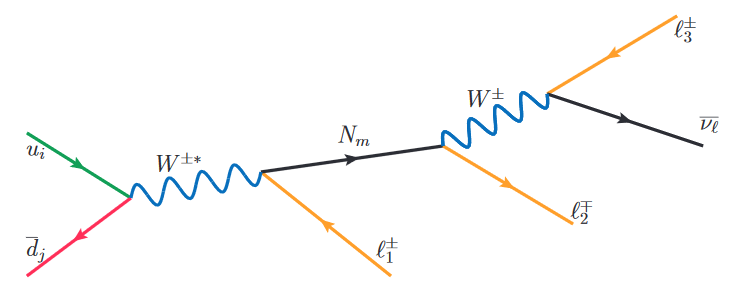
\includegraphics[width=0.9\linewidth]{ModelProcess.png}
		\caption[The charged current Drell-Yan process.]{The Born diagram for the charged current Drell-Yan process of the proton-proton collision (on the left) producing a heavy pseudo-Dirac neutrino $N$ in the inverse seesaw mechanism model, leading to a trilepton plus missing transverse energy (a light neutrino) final state. Figure is taken from ref. \cite{inverseseesaw}. \label{fig:ModelProcess}}
	\end{figure} 

	The decay products of such particle collisions can be detected in experiments like the \acrshort{lhc} and \acrshort{atlas} (sect.\ref{sect:Theory-ATLAS}). These events can also be simulated, meaning that we can simulate proton-proton collision events and the decay processes. For each decay final state product, we can measure many properties like momentum, the transverse momentum, the polar angle and the azimuthal angle. We can also detect which final state particles are produced. With these particle properties we can calculate the angles and angular distances between each produced particle, and for truth we have all the information about the neutrino (\acrshort{met}). In a real detector, we only have the transverse information\footnote{I.e. no $p_z$ and no $\theta$.}. We can also calculate the invariant masses of pairs of combined final state particles. We should then be able to find out which lepton comes from which decay branch (vertex) in the decay process in Figure \ref{fig:ModelProcess} computationally.
	
	The end goal is to identify the decay vertices (according to Fig. \ref{fig:ModelProcess}), by utilizing the particle properties in various machine learning algorithms. We will look more into machine learning in chapter \ref{chap:Theory-Machine_learning}. The data we are analyzing are covered in section \ref{sect:Method-Data}.
	

%----------------------------------------------------------------------

	\chapter{Proton-Proton Collisions}
	\label{chap:Theory-Proton_collisions}
	In this thesis we study the proton-proton (p-p) collisions from \acrshort{lhc} (sect.\ref{sect:Theory-LHC}). Protons consists of quarks and this makes proton-proton collisions somewhat complex. When two hadrons collide, it is the constituents of the hadrons\footnote{The partons, i.e. quarks and gluons.} which collide. The colliding partons only carry fractions of the total momentum of the protons. We use the center-of-mass (\acrshort{cm}) frame of the p-p collision system and not the \acrshort{cm} frame of the patrons that collide. This chapter explains the basics of high energy proton-proton collisions.

%----

	\section{Particle Kinematics}
	\label{sect:Theory-Part_kinematics}
	To describe the kinematics of what happens in p-p collisions, we need the momentum, energy and rest mass of the particles. The Einstein energy-momentum relation in natural units becomes 
	\begin{equation}
	\label{eq:Kinetics_Einstein}
		E^2=p^2+m^2.
	\end{equation}
	Since the protons will reach very high velocities when they collide, we need to include special relativity into the equations\footnote{In natural units.}:
	\begin{equation}
	\label{eq:Kinematics}
		E=\gamma m \quad \text{and}\quad \textbf{p}=\boldsymbol{\beta}\gamma m
	\end{equation}
	These equations depend on the Lorentz factor
	\begin{equation*}
	\label{eq:Lorentz_factor}
		\gamma=\frac{1}{\sqrt{1-\beta^2}}\quad \text{and} \quad \beta=\frac{v}{c}.
	\end{equation*}

	We then introduce the momentum as a four-vector momentum \[P^{\mu}=(E,\textbf{p})=(E,p_x,p_y,p_z).\] The scalar product of the four-momentum is then a Lorentz-invariant quantity
	\begin{align}
	\label{eq:Four-momenta}
		P^2=P^{\mu}P_{\mu}&=E^2-\textbf{p}^2\\
		&=\gamma^2m^2-\beta^2\gamma^2m^2 \nonumber\\
		&=m^2,\nonumber
	\end{align} 
	since the momentum and energy are conserved separately, the four-momentum is also conserved. By rearranging this equation, we just end up with the Einstein energy-momentum relationship in equation \ref{eq:Kinetics_Einstein}. This is a very useful relation in particle collisions.
	

	\subsection{Colliding Particles}
	\label{subsect:Theory-Part_colliding}
	The reference frame of choice for colliding particles, is as mentioned the \acrshort{cm} frame of the two colliding particles. This is defined where the sum of the three-momenta \textbf{p} is zero. When two particles collide, this means that $\textbf{p}_1=-\textbf{p}_2$. And when these two particles have the same rest mass $E_1=E_2=E$, we get
	\begin{equation}
	\label{eq:Four-mom_equal_E}
		(P_1+P_2)^{\mu}=(2E,\textbf{0}).
	\end{equation}
	Now we introduce what is called a Mandelstam variable\cite{thomson2013modern}, $s$ , which is defined as the squared sum of the four-momenta
	\begin{equation}
	\label{eq:Mandel_var_s}
		s=(P_1+P_2)^2.
	\end{equation}
	This we have already found out is a Lorentz-invariant quantity. We can then draw two conclusions; 1) $s$ is a Lorentz-invariant quantity as well, and 2), the $\sqrt{s}=2E$ can be interpreted as the total energy of the \acrshort{cm} system. This is a key quantity in particle physics for particle colliders.

	From equation \ref{eq:Four-momenta}, we got that $P^2=m^2$. This means that if the colliding particles were elementary particles, $\sqrt{s}$ could be interpreted as the possible energy available for heavier particle production. This would then be an upper limit for producing a heavy particle with mass $M$, as $M\leq\sqrt{s}$. But since protons are not elementary particles and the p-p collisions are really collisions between partons, this limit changes. We denote the momenta carried by the two partons colliding as $\textbf{q}_1$ and $\textbf{q}_2$. The associated four-momenta for the partons are $Q_1^{\mu}$ and $Q_2^{\mu}$. Since we mentioned that the partons only carry fractions of the momenta, these fractions will be defined as $x_1$ and $x_2$ for the two colliding partons. By using what is called the Drell-Yan process\footnote{This is not restricted to Drel-Yan processes, but yields for any 2->1 process.} (explained and derived in \citet{thomson2013modern}) for a quark and an antiquark, we get the fractions given as
	\begin{equation}
	\label{eq:Drell-Yan_fractions}
		x_1=\frac{q_1}{E}\quad \text{and}\quad x_2=\frac{q_2}{E}.
	\end{equation}

	To get the mass $M$ of a produced particle from the collision with the partons, we use the same limit as for an elementary particle collision and equation \ref{eq:Mandel_var_s} for $s$:
	\begin{align*}
		M&\leq\sqrt{s}\\
		M^2&\leq s\\
		M^2&\leq (Q_1+Q_2)^2=E^2\left[(x_1+x_2)^2-(x_1-x_2)^2\right]\\
		&=4x_1x_2E^2\\
		&=x_1x_2s
	\end{align*}
	This leads to that the produced invariant mass is equal to the \acrshort{cm} energy of the colliding partons.	

	The actual values of the fractions are described by the parton distribution functions (\acrshort{pdf}s). These \acrshort{pdf}s can be interpreted as the probability of a parton with a special flavor to carry the fraction $x$ of the proton momentum when the parton participates in a hard scattering process. 

	From this section, we can see that the event kinematics in hadron-hadron collisions have to be explained by the three independent kinematic variables, $Q^2$, $x_1$ and $x_2$.


	\subsection{Products of Particle Collisions}
	\label{subsect:Theory-Collision_products}
	In particle colliders, like at the \acrshort{lhc}, the direction of the particle beams are normally defined in the $z$-direction which gives $\textbf{p}=(0,0,p)$. This plane is the longitudinal plane. The positive $y$-direction is defined upwards, and the positive $x$-direction is defined towards the center of the ring. We can then define the transverse momentum $p_T$ perpendicular to the $z$-axis as
	\begin{equation}
	\label{eq:Transvesre_p}
		p_T=\sqrt{p_x^2+p_y^2}.
	\end{equation}
	The corresponding transverse energy is given as 
	\begin{equation}
	\label{eq:Transverse_E}
		E_T=\sqrt{p_T^2+m^2}.
	\end{equation}
	The total momentum can then be derived as 
	\begin{equation}
	\label{eq:Total_mom}
		p=\sqrt{p_T^2+p_z^2}.
	\end{equation}
	The reason for working in the transverse ($xy$) plane of the initial beam direction, is that the initial momentum is zero in this direction. We want to express the kinematics in spherical coordinates in terms of the polar angle $\theta$ and the azimuthal angle $\phi$. 

	After the collisions, not just the parton jets, but the whole system will get a boost along the beam direction. That is why we introduce a \textit{rapidity} variable $y$ that is used to express the jet angles:
	\begin{equation}
	\label{eq:Rapidity}
		y=\frac{1}{2}\ln\left(\frac{E+p_z}{E-p_z}\right)
	\end{equation}
	What is useful with this rapidity variable, is that the rapidity differences are invariant under Lorentz boosts along the beam direction. This does not apply for the polar angle $\theta$. 

	If the particle mass is small compared to the particle energy, $p_z\approx E\cos\theta$. We can then rewrite the rapidity as
	\begin{equation}
	\label{eq:Pseudorapidity}
		y\approx\frac{1}{2}\ln\left(\frac{1+\cos\theta}{1-\cos\theta}\right)=\frac{1}{2}\ln\left(\cot^2\frac{\theta}{2}\right)=-\ln\left(\tan\frac{\theta}{2}\right)\equiv\eta
	\end{equation}
	This new variable $\eta$ is called the \textit{pseudorapidity}. The pseudorapidity also has the following relation with the polar angle: $\eta(\theta)=-\eta(180\text{\textdegree}-\theta)$. We now have the most used set of variables ($p_t, \phi, \theta$) for describing the kinematics of particles in a detector. In Figure \ref{fig:Planes} we see the illustration of the transverse and longitudinal planes. The cylindrical shape shows how particle accelerators will be situated around the collision point.
	\begin{figure}[htbp!]
		\hspace*{-1.6cm}
		\subfloat[The transverse plane.]{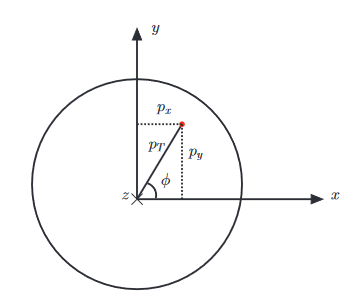
\includegraphics[width=0.6\linewidth]{Transverse.png}}
		\subfloat[The longitudinal plane.]{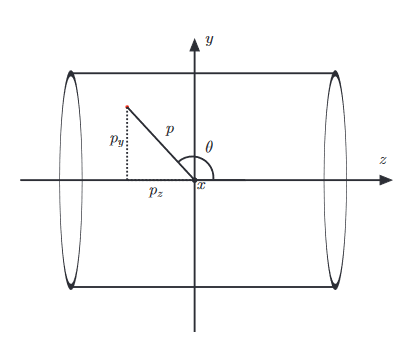
\includegraphics[width=0.6\linewidth]{Longitudinal.png}}
		\caption[Collider geometry.]{Illustrations of the (a) transverse plane and the (b) longitudinal plane. The collision point is at the origin. Figures are both from ref. \cite{gramstad2013searches}. \label{fig:Planes}}
	\end{figure} 

	Another useful variable associated with hadron colliders, is the angular distance between two particles
	\begin{equation}
	\label{eq:Angular_distance}
		\Delta R=\sqrt{(\Delta \eta)^2+(\Delta \phi)^2}.
	\end{equation}
	The angular distance defines how much two particles are moving in the same direction or as the separation in the $\phi\eta$-space, and is invariant under longitudinal boosts.

%----

	\section{Proton-Proton Interactions}
	\label{sect:Theory-P-P_interactions}
	When proton-proton collisions take place in colliders, the interactions can roughly be divided into three groups:
	\[\text{i) elastic (el)}\quad \text{ii) diffractive (di)}\quad \text{iii) non-diffractive (nd)}\]
	These three groups are also components that make up the total cross-section at proton-proton colliders:
	\begin{equation}
	\label{eq:Cross-section}
		\sigma_{\text{total}}=\sigma_{el}+\sigma_{di}+\sigma_{nd}
	\end{equation}
	For elastic processes, both the colliding protons remain unchanged. For the diffractive processes (di and nd), the collisions/interactions are inelastic and one or both protons will be fragmented. This leads to multi-particle final states. 
	
	The elastic and diffractive interactions have cross-sections that can not be calculated using perturbation theory, meaning they are non-perturbative processes. In these cases we get so-called \textit{pomerons}, which are color singlet states that do not exchange color between the protons. These interaction processes at high-$p_T$ proton-proton collisions are normally not interesting, since they will produce particles with low transverse momentum close to the beam line. They are thus difficult to detect, but important for luminosity measurements since they contribute to the total p-p cross-section. These events are detected in special experiments that use \textit{minimum bias} events, where the final state has no requirements or special triggers. 
	
	
	\subsection{Hard Scattering Events}
	\label{subsect:Theory-Hard_scattering}
	The more interesting events to look at in high-$p_T$ p-p collisions, are the non-diffraction events. With non-diffractive events, there is an exchange of color between the partons in the interaction. These are called hard scattering events. Hard scattering events with high momentum transfers, $Q^2$, may create heavy particles. This is the main interest in particle colliders. 
	
	A hard scattering event can be expressed as
	\begin{equation}
	\label{eq:Hard_scattering}
	A+B\rightarrow c+X,
	\end{equation}
	where the collision between the partons are expressed as
	\begin{equation}
	\label{eq:Hard_scattering_partons}
	a+b\rightarrow c.
	\end{equation}
	$A$ and $B$ are the two colliding protons, and $a$ and $b$ are the corresponding colliding partons. $c$ are the interesting high $p_T$ objects. $X$ are underlying products which are mostly remnants after the original collision.
	
	In Figure \ref{fig:HardScattering} we see how a hard scattering p-p collision may look like, with outgoing partons, underlying events, initial- and final-state radiation. The initial-state radiation is mean radiation of gluons or photons from partons before the hard scattering. Final-state radiation is the mean radiation from the produced partons after the hard interaction. The underlying events are the further interactions between partons beyond the hard scattering. These interactions will often go out of reach of the detector, and is another reason why we look at the transverse plane.
	\begin{figure}[htbp!]
		\hspace*{-1.0cm}
		\centering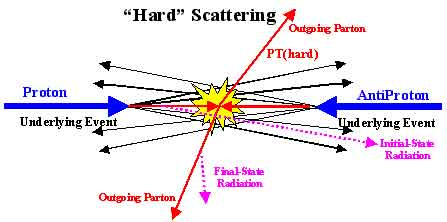
\includegraphics[width=0.9\linewidth]{HardScattering.png}
		\caption[Hard scattering.]{Illustration of a hard scattering proton-proton collision. Figure is taken from ref. \cite{field2002hardscattering}. \label{fig:HardScattering}}
	\end{figure} 
	
	
	\subsection{Parton Distribution Function}
	\label{subsect:Theory-PartonDF}
	The parton distribution function (\acrshort{pdf})\footnote{See chapter 8 in \citet{thomson2013modern} for more in depth explanations.}  is used to describe the probability density of the two partons, $a$ in proton $A$ and $b$ in proton $B$, to carry the proton momentum fractions $x_a$ and $x_b$. These \acrshort{pdf}s are also dependent on the squared of the momentum scale indicating the total four-momentum transfer in the collisions $Q^2$ as $F_{a/A}(x_a,Q^2)$ and $F_{b/B}(x_b,Q^2)$. These PDFs must be found experimentally in Deep Inelastic Scattering (\acrshort{dis}) experiments of leptons against hadrons, since they cannot be calculated from \acrshort{qcd} theory. The \acrshort{pdf}s are also used to get the cross-section of the collisions. 
	
	With the measured \acrshort{pdf}s $f(x,Q^2)$, a structure function $F_2^{ep}(x,Q^2)$ can be determined
	\begin{equation}
	\label{eq:Structure_function}
	F_2^{ep}(x,Q^2)=2xF_1^{ep}(x,Q^2)=x\sum_{i}Q_i^2f_i(x),
	\end{equation}
	where $i$ is a quark in the proton and $Q_i$ is the charge of the quark. The interesting here are the $f(x)$ of each of the partons. So results of measurements from several \acrshort{dis} experiments of varying structure functions, which are superpositions of the same $f_i(x)$'s, are combined to get the $f(x)$ for each parton.
		
	
	\subsection{Hadronization}
	\label{subsect:Theory-Hadronization}
	We already have covered that quarks and gluons carry color charge (sect. \ref{sect:Theory-Particles}), and that they are not observed as free particles\footnote{Only exception is the top quark with shorter lifetime than the QCD interaction time scale.}. They can only be found in colorless objects like hadrons. 
	
	We also talked about the strong force, which increases in strength when increasing the distance between (elementary) particles. So if we separate a quark from a hadron, the color field will increase and the emerged energy will enable creation of new quark-anitquark pairs or gluons. These will be observed as jets of colorless particles. As this production of partons continue, the energy will decrease until it is low enough to produce hadrons. This process of high-energy quarks (and gluons) that produce new jets until we get hadrons, is called \textit{hadronization}. The jets can also be called hadronic showers, since many hadrons are usually produced in hadronization processes.
	
	Jets are not only produced in p-p collisions with hard scattering, but also in the underlying events and from initial- and final-state radiation. This makes p-p collisions very complicated and messy when trying to study them, compared to electron-positron collisions.	
	
%----------------------------------------------------------------------
	
	\chapter{Particle Accelerators and Collider Experiments}
	\label{chap:Theory-Part_accelerators}
	To fully understand the physics of the particles around us and what the Universe is made of, we need some way of looking at the subatomic world. This is done in huge particle accelerators where particles are accelerated to high velocities and energies, and collided with each other to make other particles. Here the aftermath of the collisions result in new particles with new energies that are detected as they move through detectors. 
	
	There are various accelerators and detectors which produce and accelerate different particles in the world. In this chapter we will look at the biggest particle physics laboratory in the world, namely the European Organization for Nuclear Research (\acrshort{cern}\footnote{The name CERN is originally from French; Conseil Européen pour la Recherche Nucléaire.}), and some of its components like particle accelerators and detectors.
	
%----

	\section{CERN}
	\label{sect:Theory-CERN}
	The \acrshort{cern} laboratory lies near Geneva, on the border between France and Switzerland, and was founded in 1954 \cite{AboutCERN}. It is a multinational collaboration between 23 (mostly) European countries. They also have several international relations with other countries both inside and outside of Europe. \acrshort{cern}s main focuses today is particle physics and particle accelerator experiments. Many of the biggest discoveries in particle physics have come from particle experiments at \acrshort{cern}. This includes, among others, the discovery of the Higgs boson and discovery of the $W$ and $Z$ bosons. At the main site of \acrshort{cern} in Meyrin, and in the World LHC Computing Grid (\acrshort{wlcg}) scattered around the world, data of simulations of particle collisions are stored. \acrshort{cern} is the place where Tim Berners-Lee invented the World Wide Web in the late 1980s \cite{mcpherson2009WWW}.
	
	\acrshort{cern} consists of several particle accelerators, experiments and facilities in different shapes and sizes. The two main types of accelerators are linear and circular. They are located at various sites, and they accelerate particles to high energies before they send the particles to be collided with other accelerated particles or particles with stationary targets, or are sent to more powerful accelerators. They are built differently to accelerate different kinds of particles with different masses. In Figure \ref{fig:CERN_Layout} we see the \acrshort{cern} accelerator complex. Some of the accelerators are mostly used to pre-accelerate the particles before they are sent to another accelerator where they are accelerated even more. This repeats until the particles reach the desired energy to collide with at one of the detectors.
	\begin{figure}[htbp!]
		\centering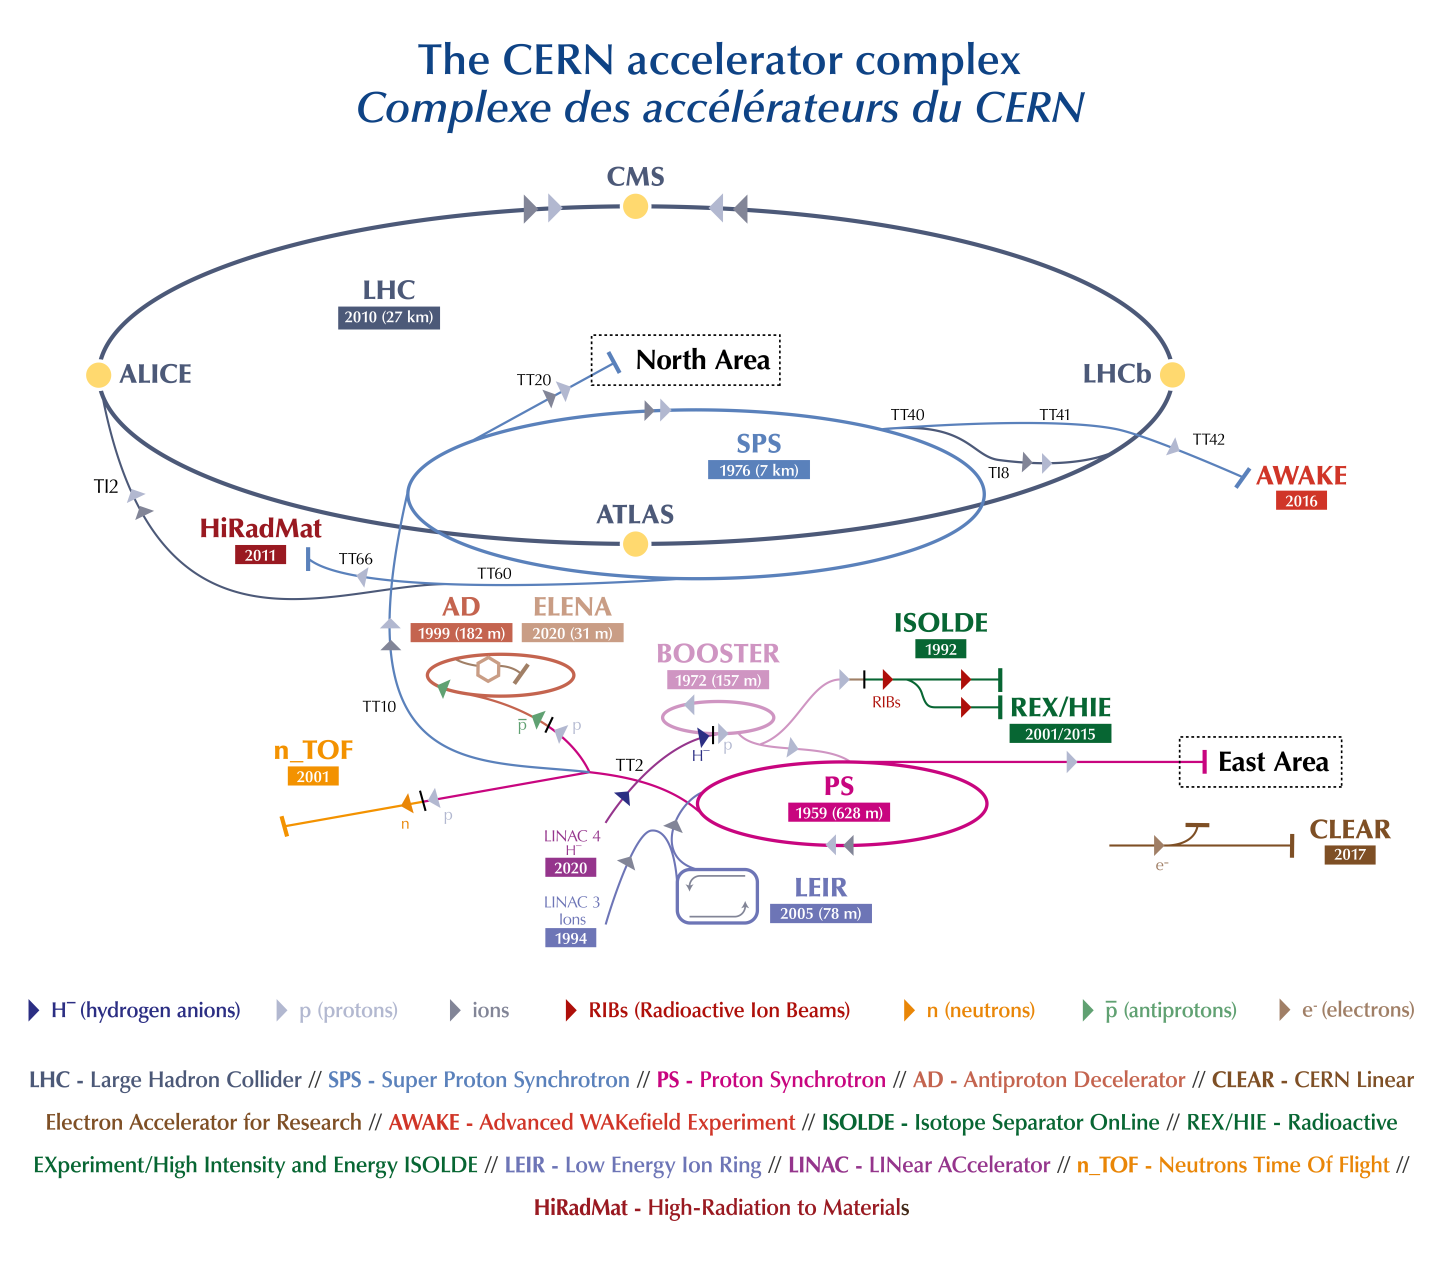
\includegraphics[width=1.1\linewidth]{CERN_layout.png}
		\caption[The CERN complex.]{The CERN accelerator complex as of 2019. Credit: CERN\cite{MobsCERNLayout}.\label{fig:CERN_Layout}}
	\end{figure} 

	For the more important discoveries, like the ones we have mentioned above, the $W$ and $Z$ bosons were discovered by the Super Proton Synchrotron (\acrshort{sps}) in 1983. The \acrshort{sps} delivered an energy between 300-450 GeV. It was then later used to accelerate high energy electrons and positrons into the Large Electron-Positron Collider (\acrshort{lep}). \acrshort{lep} is the largest and most powerful lepton collider built to this date, and was functional between 1989 and 2000. \acrshort{lep} was then replaced by the Large Hadron Collider (\acrshort{lhc}) in 2008 to collide protons and heavy ions. 
	
%----

	\section{The LHC and Accelerator Experiments}
	\label{sect:Theory-LHC}
	Today's largest and most powerful particle accelerator is the Large Hadron Collider (\acrshort{lhc}) \cite{LHCatCERN}, which we easily can see in Figure \ref{fig:CERN_Layout} as the biggest gray circle around the North Area. The particles are sent in bunches up to $10^{11}$ protons and are accelerated using radio frequency cavities in a 27 km ring consisting of superconducting magnets, where the particles are boosted in several structures along the ring to the desired energies. The \acrshort{lhc} is designed to have 2808 bunches at the same time traveling in the ring. The ring lies 100 m underground in a tunnel beneath the French-Swiss border. Along the ring, there are 4 main crossing points (\acrshort{atlas}, \acrshort{cms}, \acrshort{alice}, \acrshort{lhcb}) with detectors that register the particle collisions and the following particle decays. At these collision points, the total collision energy, or center-of-mass energy $\sqrt{s}$, can reach 13 TeV\footnote{The LHC is theorized to a limit of 14 TeV.}. There are in total seven detectors along the ring, each designed for different experiments.
	
	The \acrshort{lhc} was first used for proton-proton (hadron) collisions in 2010 (run 1), where it reached a record high energy of 3.5 TeV per beam. After upgrades, during run 2, it reached an even higher energy of 6.5 TeV per beam. It is currently stopped for another upgrade, which started in 2018 and is during operation. The accelerator sends two high-energy beams, in separate tubes and directions, near the speed of light before they collide at one of the detectors. To reach these high energies, the particle beams are accelerated in several systems which increase the energies before injected into the main \acrshort{lhc} ring \cite{AccatCERN}. Inside the tubes, there is an ultrahigh vacuum. To make sure that the particles are directed correctly through the ring, superconducting electromagnets are used to bend the particle trajectories. The magnets vary in strengths and sizes to direct the beams properly. Since the particles are incredibly tiny, the precision of the magnets have to be extremely good to make the particles hit each other at the collision points. That is also why beams of $10^{11}$ protons are accelerated and not single particles. Since the construction of the accelerator is a ring they can continue around again when some of them do not collide. A beam can typically go around in the ring for about 10 hours before the beam has lost too much intensity.
	
	As mentioned earlier, there are seven detector experiments at the \acrshort{lhc} \cite{DetectorsatCERN}. The four main, and biggest, detectors in the \acrshort{lhc}, have different objectives. The \acrshort{atlas} and \acrshort{cms} experiments are two large and similar general-purpose particle detectors that looks for new physics and more precise study of the \acrshort{sm}. The \acrshort{alice} and \acrshort{lhcb} experiments have more specific roles, and study the quark-gluon plasma from heavy ion collisions and missing antimatter connected to CP-violation after the Big Bang, respectively. The remaining detectors are much smaller and are used in more specialized research. We will look more at the \acrshort{atlas} detector later (sect.\ref{sect:Theory-ATLAS}).
	
	The \acrshort{lhc} is used to explore many different open questions in physics, like to further study the \acrshort{sm} and theories beyond it. In addition to proton-proton collisions, the \acrshort{lhc} can also collide heavy ion collisions at some of the detectors. 	
	
	
	\subsection{Important Parameters}
	\label{subsect:Theory-Important_params}
	One of the most important parameters of measurements at particle accelerators, is the \acrshort{cm} energy $\sqrt{s}$ we already have mentioned. For two particles colliding, the Lorentz invariant quantity $s$ (the squared invariant mass) is formed as
	\begin{equation}
	\label{eq:s_accelerators}
		s=\left(\sum_{i=1}^2E_i\right)^2-\left(\sum_{i=1}^2\textbf{p}_i\right)^2.
	\end{equation}
	
	There are also other important parameters used to describe the performance of particle colliders:
	
	
	\subsubsection{Luminosity}
	\label{subsubsect:Theory-Luminosity}
	Another important parameter in particle collider performance is the \textit{luminosity}, $\mathcal{L}$. The design luminosity of the \acrshort{lhc} is $\mathcal{L}=10^{34}$ cm$^{-2}$s$^{-1}$. The bunches at the \acrshort{lhc} are separated by 25 ns, which corresponds to a frequency of $f=40$ MHz. The (instantaneous) luminosity is used to describe the number of collisions per area per second as\footnote{With the assumption of Gaussian profile beams and head-on collisions.}
	\begin{equation}
	\label{eq:Luminosity}
		\mathcal{L}=f\frac{n_1n_2}{4\pi \sigma_x \sigma_y},
	\end{equation}
	where $f$ is the frequency of the particle beam bunches colliding (bunch crossing rate), $n_1$ and $n_2$ are the number of particles in the colliding bunches and $\sigma_x$ and $\sigma_y$ are the root-mean-square (rms) horizontal and vertical beam sizes.
	
	The complete collider luminosity at the \acrshort{lhc} can be written in terms of colliding beam parameters \cite{atlasLuminosity}
	\begin{equation}
	\label{eq:Luminosity_comp}
		\mathcal{L}=f\frac{n_1n_2n_b}{4\pi \sigma_x \sigma_y} F(\sigma_x,\sigma_y,\sigma_s,\Phi).
	\end{equation}
	This equation has the same parameters as in equation \ref{eq:Luminosity}, except for two additional parameters. $n_b$ is the number of proton bunches. $F$ is a geometrical reduction factor accounting for the non-zero-crossing angle at the interaction point, depending on the two rms beam sizes, the beam length $\sigma_s$ and the crossing angle $\Phi$.
	
	
	\subsubsection{Rate}
	\label{subsubsect:Theory-Rate}
	The cross-section, $\sigma$, for a given collision process is given by the \acrshort{sm} (or any other new model). The cross-section can be used to compute the (event) \textit{rate}, $R$, after accumulating many such collisions. The rate is calculated as
	\begin{equation}
	\label{eq:Rate}
	 	R=\sigma\mathcal{L}.
	\end{equation}
	
	
	\subsubsection{Number of interactions}
	\label{subsubsect:Theory-No_interaction}
	The total number of expected events of a given process with cross-section, $\sigma$,  over a given time, is the time integration of the event rate
	\begin{equation}
	\label{eq:No_int}
		N=\sigma\int\mathcal{L} dt.
	\end{equation}
	The time-integral of the luminosity, $\int\mathcal{L}dt$, is often called the \textit{integrated luminosity}, and is given in inverse femtobarns [$fb^{-1}$]. 
	
	
	\subsubsection{Pile-up}
	\label{subsubsect:Theory-Pileup}
	In particle collisions, we want a high instantaneous luminosity. This means that the intensity of the proton beam need to be high. But with high intensity proton beams, the probability of having more than one proton undergoing an inelastic interaction per bunch crossing is increased. This leads to what is called \textit{pile-up} events, where there are several collisions from the same bunch crossing. This means we need very accurate measurements in detection of the particle tracks to distinguish which new particles comes from which collisions. The main event that is normally used in detection, and this corresponding vertex is called the \textit{primary vertex}. 
	
	Since we want higher and higher luminosity to get more collisions, we also get more pile-ups. This need to be controlled to be able to use the data efficiently. The additional collisions do normally have smaller momentum transfers, which means we can characterize them as minimum bias events.
	
%----

	\section{The ATLAS Experiment and Particle Detection} 
	\label{sect:Theory-ATLAS}
	To detect the particles produced at particle colliders, we need different instruments that can detect the various types of particle interactions. The largest detector at the \acrshort{lhc} is the \acrshort{atlas} (A Toroidal LHC ApparatuS) experiment. In Figure \ref{fig:ATLASdetector} we see a computer generated image of the \acrshort{atlas} detector with pointers to the main components. It is 25 m in diameter, 46 m long and weights about 7000 tons. The cylindrical shape of \acrshort{atlas} is optimized to detect as many particles as possible, and covers almost a $4\pi$ angle with detectors. Like we mentioned earlier for particle collisions in the \acrshort{lhc}, \acrshort{atlas} uses the same Cartesian coordinate system with the $z$-direction in the direction of the beam, $y$-direction is upward and $x$-direction is towards the center of the accelerator circle. It also uses a spherical coordinate system with the azimuthal angle $\phi$ in the $xy$-plane around the beam axis, and the polar angle $\theta$ being the angle from the beam axis. To measure the distance between the particles, the angular distance $\Delta R$ (eq.\ref{eq:Angular_distance}) in the $\phi\eta$-plane is used.
	
	%The detector can be divided into three parts; the central part is called the \textit{barrel}, and the two end parts are called \textit{end-caps}. 
	\begin{figure}[h!]
		\hspace*{-1.2cm}
		\centering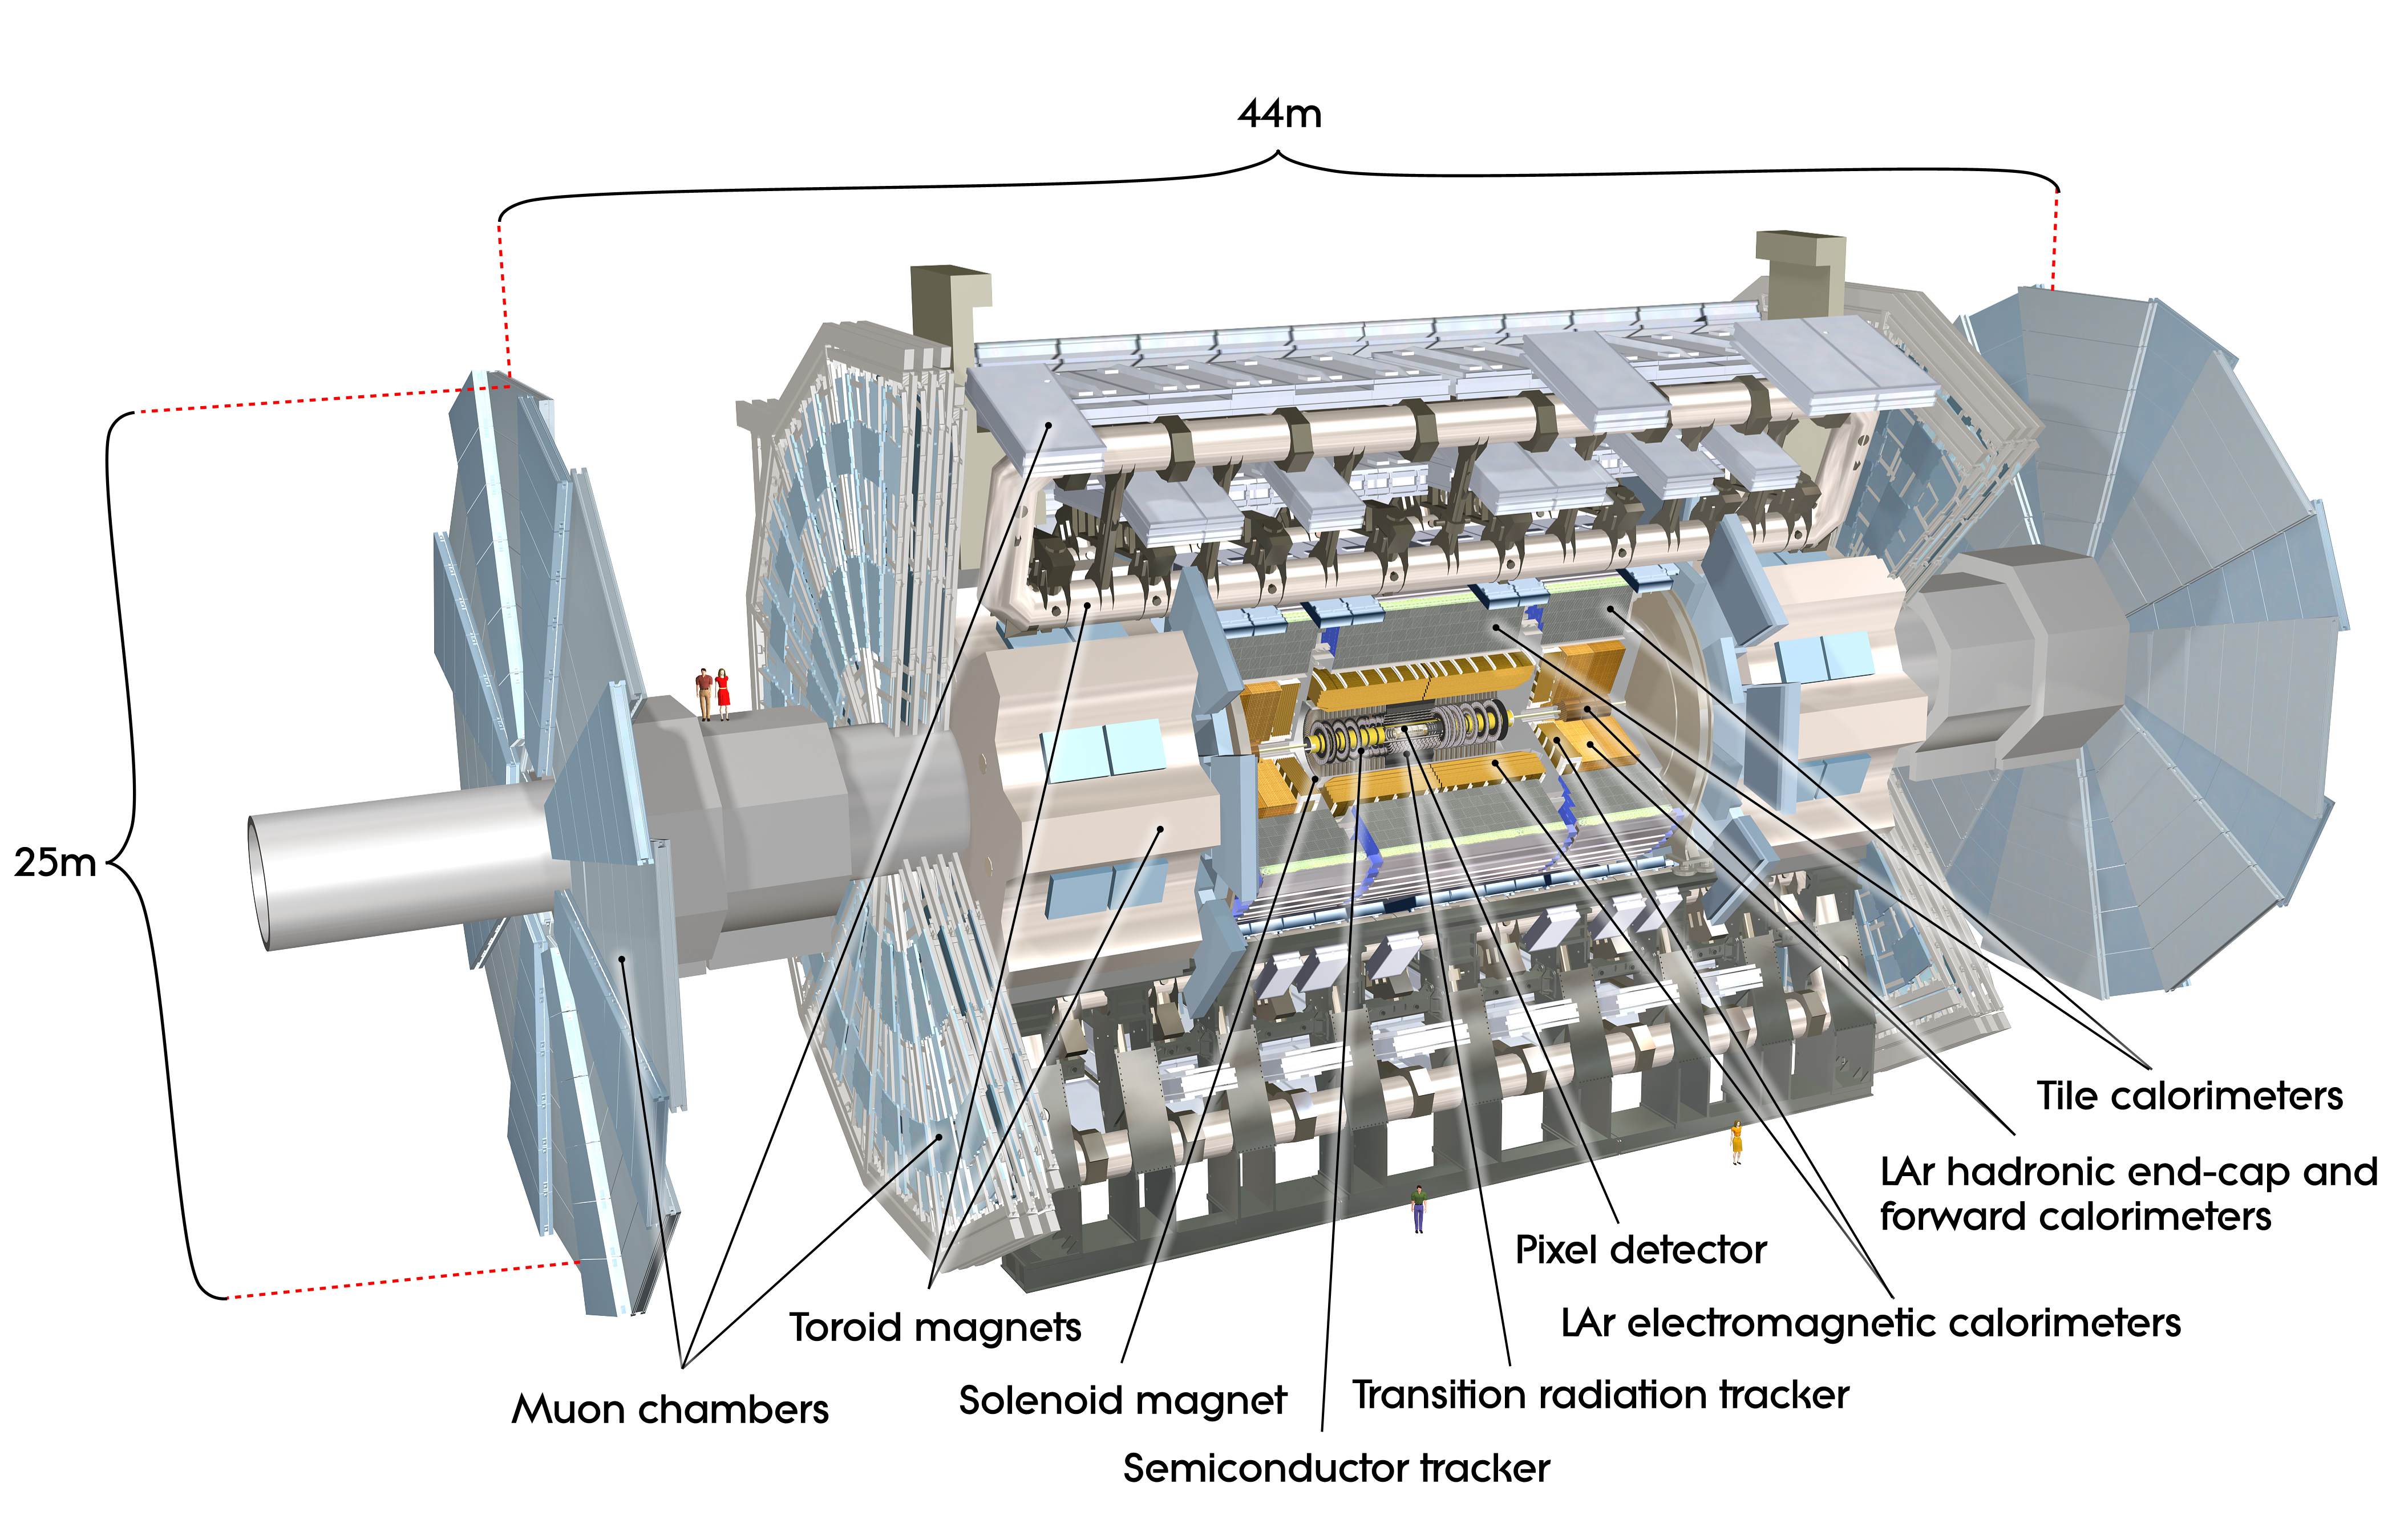
\includegraphics[width=1.2\linewidth]{ATLAS.jpg}
		\caption[The ATLAS detector components.]{The ATLAS detector and its components. Credit: \citet{ATLASdetector}.\label{fig:ATLASdetector}}
	\end{figure}  
	
	The \acrshort{atlas} detector is designed to be a general-purpose detector, covering a wide range of signals. The particle properties the \acrshort{atlas} detector can detect is the mass, momentum and energies of the particles. For \acrshort{atlas} to detect these properties, it has a layered design of detectors that is optimized in observing specific properties of the various particles. The \acrshort{atlas} detector consists of several main systems; the inner detector (\acrshort{id}), calorimeters, a muon spectrometer (\acrshort{ms}), a magnet system and a trigger and data acquisition system. The main systems consists of smaller sub-systems, which we will take a brief look at next. In Figure \ref{fig:ATLAStracking}, we see a sketch of the detector layout systems and how some particles behave in these different systems. Only the neutrinos should now go undetected through the detectors, in principle, and they are normally identified as missing momentum, or \acrshort{met}. This comes from the energy conservation law, where the sum of the measured transverse momenta of the all particles produced should be zero. 
	\begin{figure}[htbp!]
		\centering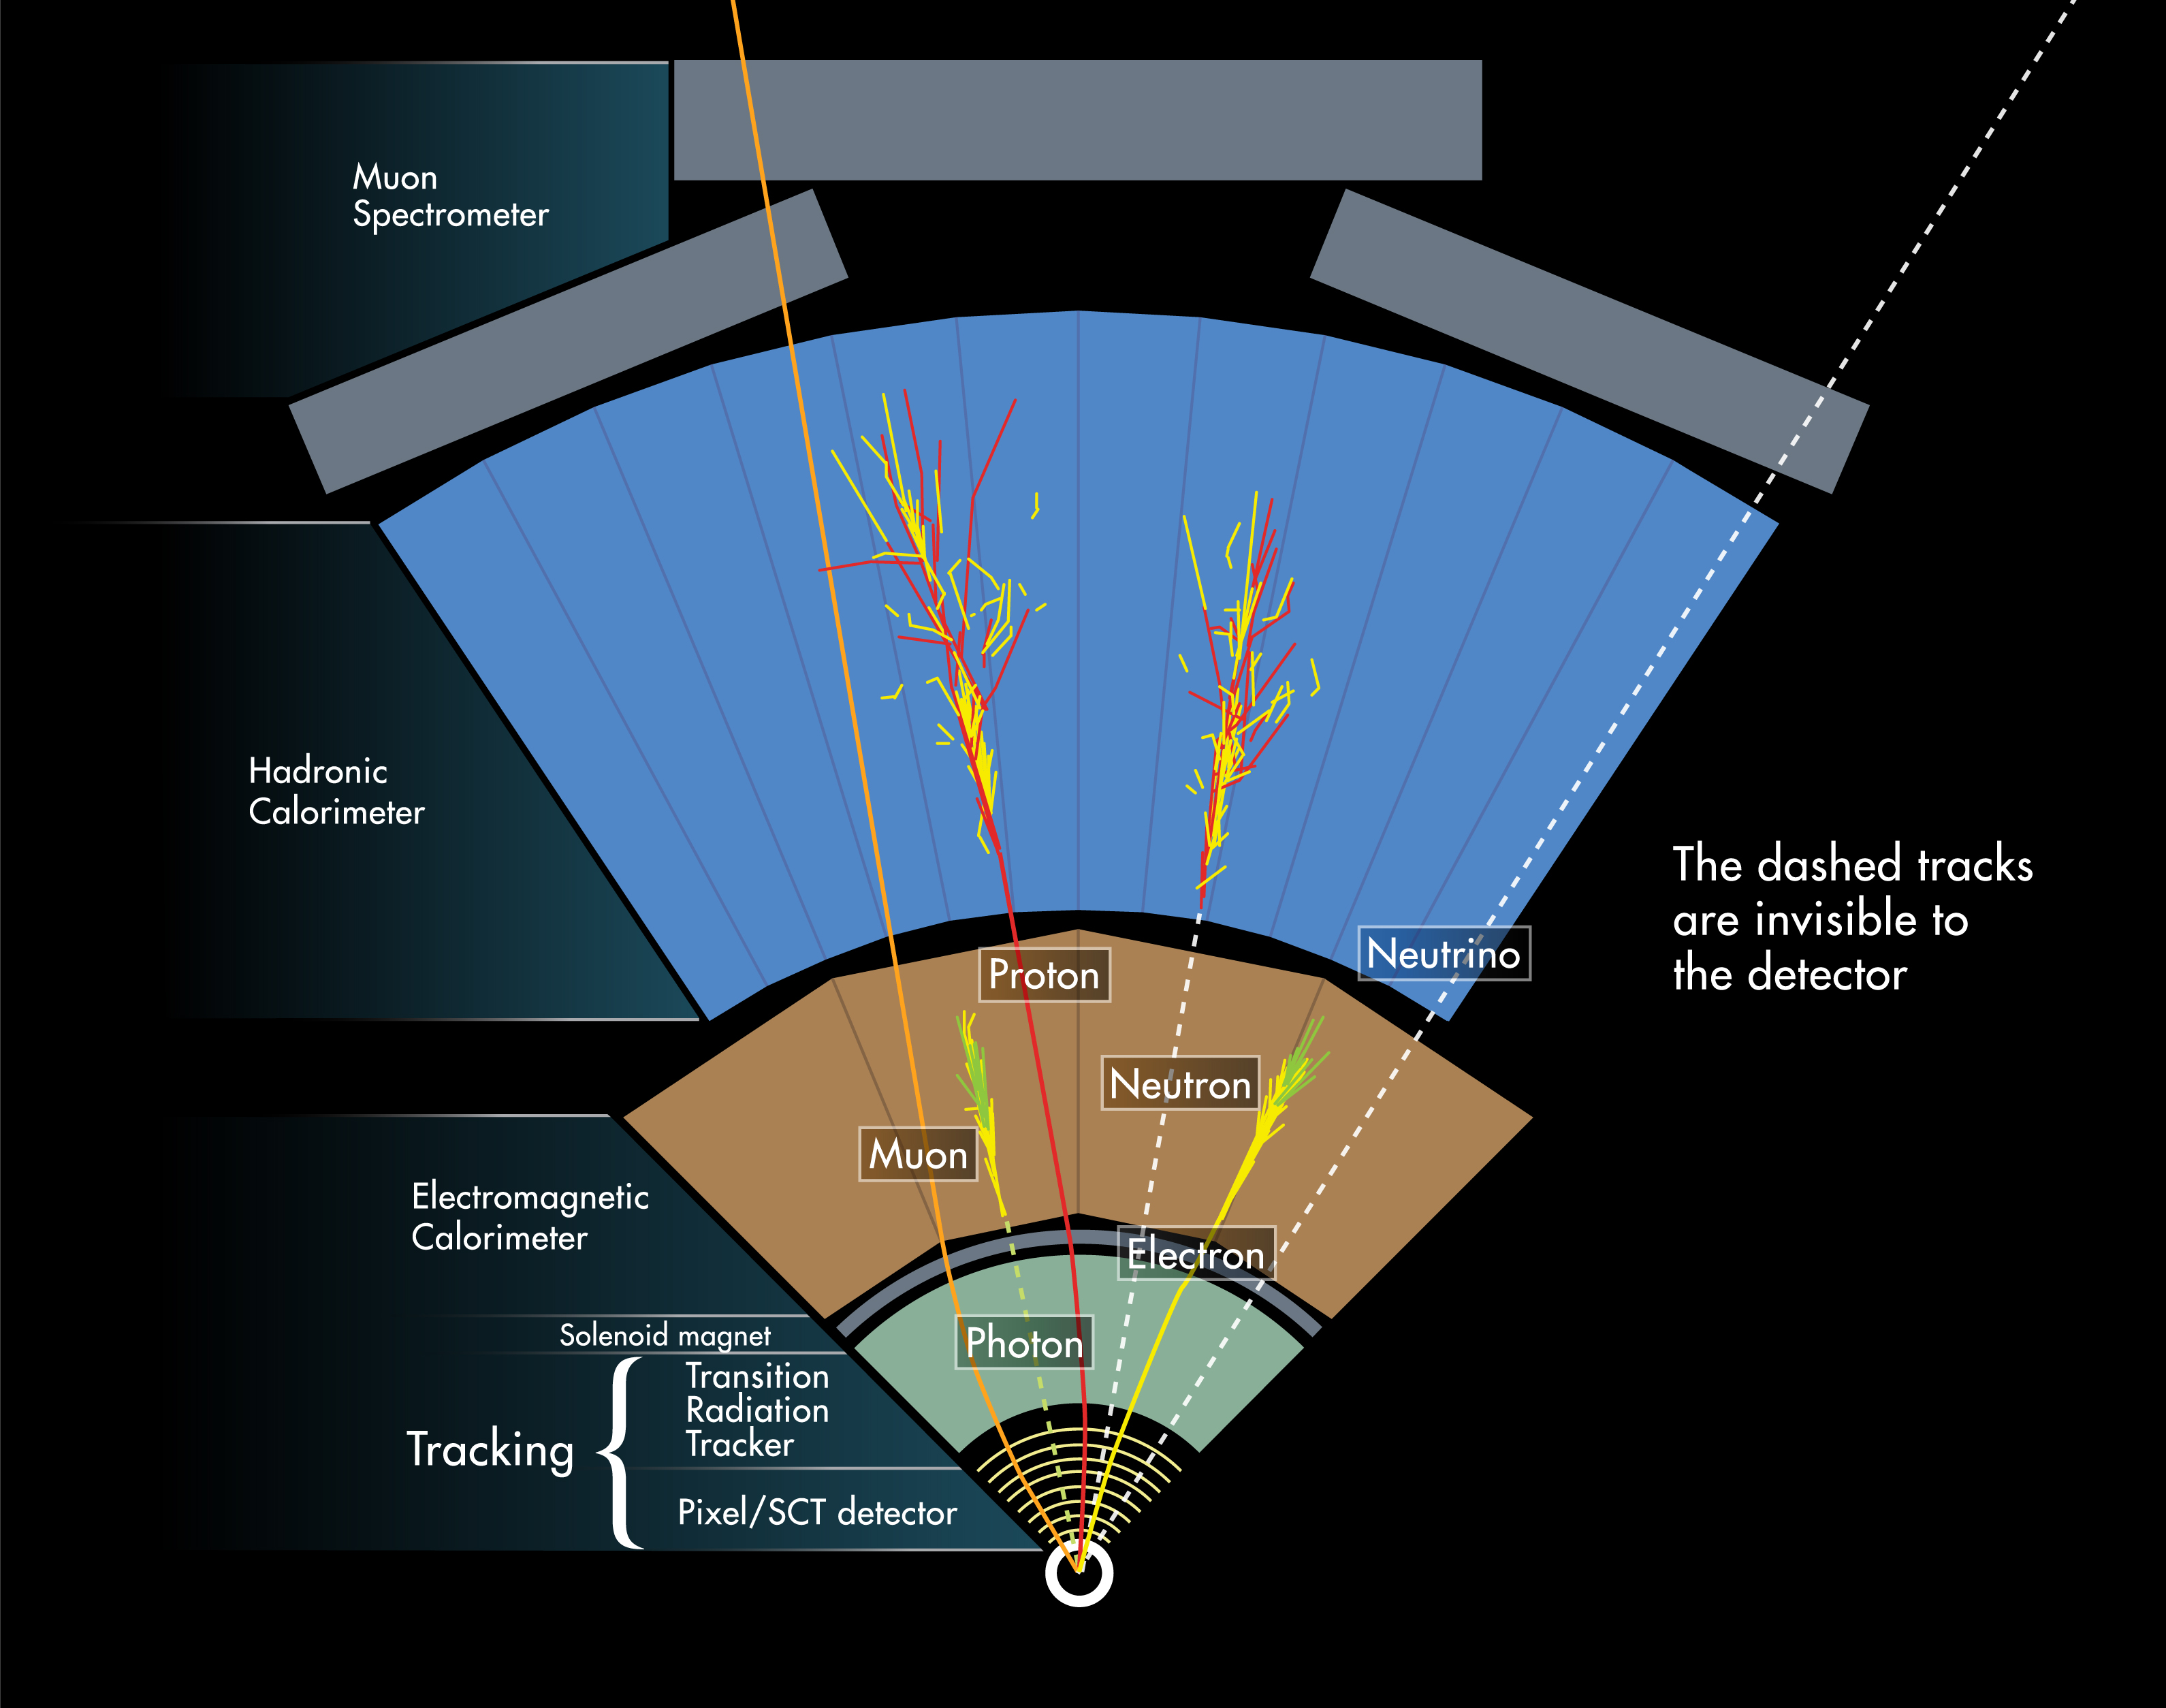
\includegraphics[width=1.0\linewidth]{ATLAS_tracks.jpg}
		\caption[The ATLAS detector tracking system.]{An illustration of the main tracking systems in the ATLAS detector, including how some particles behave in the various systems. Credit: ref. \cite{ATLAStracking}.\label{fig:ATLAStracking}}
	\end{figure} 
	
	
	\subsection{Inner Detector}
	\label{subsect:Theory-InnerDetector}
	The inner detector tracks charged particles that leaves traces of ionized atoms when traveling through a medium. The tracks, momentum and charges of the particles can be traced in a 2 T magnetic field that makes the charged particles curve. The degree of the curvature is used to determine the charge and the momentum. 
	
	The inner detector consists of three sub-systems. The inner most part is a silicon Pixel Detector that is used for extremely precise tracking near the interaction point of the particle collisions. The second part is a Semiconductor Tracker (\acrshort{sct}) that covers a bigger area than the pixel detector for the particle tracking and uses long and narrow strips instead of pixels. The third part is a Transition Radiation Tracker (\acrshort{trt}) that covers an even larger area with lower spatial resolution, and can detect transition radiation photons by using gas filled drift/straw tubes. The \acrshort{trt} provides the capability of electron identification for a variety of energies since the transition radiation gives out a stronger signal than ionization signal.
	
	%, which covers $|\eta|<2.5$.  The \acrshort{sct} provides detection in the range of $|\eta|<2.5$ as well.  It has a coverage of $|\eta|<2$.
	
	
	\subsection{Calorimeters}
	\label{subsect:Theory-Calorimeters}
	Outside the \acrshort{id} and the solenoid magnet system, there follows two types of calorimeters; an (inner) electromagnetic calorimeter and a (outer) hadronic calorimeter. Their purpose is to measure the energy of the passing particles and particle showers especially. %They both consist of a barrel part and two end-cap parts.
	
	The \textbf{electromagnetic} calorimeter (\acrshort{ecal}) measures particles that interact electromagnetically, like charged leptons and photons. The \acrshort{ecal} is made of layers of lead absorbing plates and liquid argon, and covers the whole $\phi$ angle around the beam axis. The energy is measured in the liquid argon, and free electrons are picked up by electrodes. The \acrshort{ecal} is covered by cryostats to keep it at the correct low temperature. %The thickness of the \acrshort{ecal} is measured in radiation lengths $X_0$, which is the mean length required to reduce the energy of a particle by $1/E$ in a material. The thickness of the barrel part is $\geq22X_0$, while the end-caps are $\geq24X_0$.
	
	The \textbf{hadronic} calorimeter (\acrshort{hcal}) measures hadrons and hadronic showers\footnote[14]{It measures the energy of particles that interact via the strong force, which is mainly hadrons.}. The \acrshort{hcal} is made of several layers of steel absorbers and plastic scintillator tiles that alternates. The iron in the detector both slows down and traps hadrons. The \acrshort{hcal} is a lot bigger than the \acrshort{ecal}. 
	%The \acrshort{hcal} consists of three parts.  The \acrshort{hcal} is not as precise as the \acrshort{ecal}. The thickness of the \acrshort{hcal} is measured in interaction lengths $\lambda$, which is the mean distance a particle travels before interacting strongly with the material. The detector is 9.7 interaction lengths thick \cite{aad2008atlas}.
	
	
	\subsection{Muon Spectrometer}
	\label{subsect:Theory-MuonSpectrometer}
	Outside the calorimeters, we find the muon spectrometer. Here high-energy muons are detected. This detector is very large, 11 m radius \cite{ATLAS_Muon_spec}, and consist of three parts; a magnetic field with several toroidal magnets, a set of chambers measuring the tracks of the muons and a set of triggering chambers with accurate time-resolution. The detection of the muons happens the same way as before, by measuring their momentum as they are bent in the detector. They should also be simpler to identify since all other identifiable particles should not reach this far out from the interaction point.
	%as well as a barrel and two end-caps 
	
	
	\subsection{Magnet System}
	\label{subsect:Theory-MagnetSystem}
	\acrshort{atlas} uses two types of superconducting magnet systems to measure the momentum from the bending of the particles through the Lorentz force. The magnet system consists of a central solenoid, a barrel toroid and two end-cap toroids. The central solenoid is located between the inner detector and the electromagnetic calorimeter, which produces the 2 T magnetic field for the \acrshort{id}. The barrel toroid produces a magnetic field of 0.6 T, and is located around the middle cylinder of the \acrshort{ms} barrel outside the calorimeters. The two end-cap toroids produce magnetic fields of 1 T, and are located at the end-cap regions of the Muon System.
	
	
	\subsection{Trigger System}
	\label{subsect:Theory-TriggerSystem}
	The detector produces a huge amount of data, which need to be stored and processed. The output event storage rate have to be reduced from an initial bunch crossing of 40 MHz to $\sim$200 Hz. To only get the most interesting data for further analysis, a trigger system is used to extract these relevant events. The ATLAS Trigger and Data Acquisition system (\acrshort{tdaq}) has three levels for reducing the amount of stored data \cite{scannicchio2010atlas}; the Level 1 (LVL1) trigger is hardware-based and makes quick decisions of which events to store, the Level 2 (LVL2) and the Event filters (\acrshort{ef}) are software-based and are often combined to and referred to as the High Level Triggers (\acrshort{hlt}). Only the events passing both the LVL1 and \acrshort{hlt} are stored for further analysis.
	
	The LVL1 trigger uses information from the calorimeters and the muon spectrometer to choose interesting events. These interesting events passed on to the next trigger. The LVL1 trigger also defines regions based on the $\phi$ and $\eta$ coordinates from the interesting events.
	
	The LVL2 trigger uses all the information within the regions of interest (\acrshort{roi}s) defined by the LVL1 trigger to further reduce the amount of event data. The accepted events are then assembled put together into a full event. The \acrshort{ef} uses an offline analysis to even further reduce the data used to store and further analysis at the \acrshort{wlcg}. 


%----------------------------------------------------------------------	
	
	\chapter{Machine Learning}
	\label{chap:Theory-Machine_learning}
	\section{Introduction}
	\label{sect:Theory-IntroML}
	Machine learning (\acrshort{ml}) has recently become widely used in many fields of research. The meaning of machine learning is to train computational algorithms to automatically determine an outcome from specific patterns in data the algorithms have not seen before by using pre-trained algorithms with a given input set of hyperparameters. When training an algorithm, one tries to teach patterns using large amounts of data. \acrshort{ml} goes in under what is called artificial intelligence, which is where the computer takes its own decisions to produce and predict solutions to problems. 
	
	The machine learning algorithms build a model based on some given data and general rules. The data may often need to be processed in some way, like when there are missing values in the data set. The models are then fit and trained on sample data, which is a subset of the full data set. The remaining data, which is a smaller part than the training data, are used to make predictions and do an evaluation of the trained model. There is a huge variety of different evaluation metrics which are used to check the performance of the algorithms on data. When we have a good enough trained model, we can save it and use it later on similar unseen data.
	
	There is a plethora of usages for machine learning, and it is often divided into estimation or prediction problems. An example of a machine learning problem can be to identify objects in images of animals, which may be easy to humans. Algorithms can be trained to identify various animals by the algorithms given some features to best distinguish the animals from each other. This may be the shape of ears or the tail of the animals. Computationally this means we choose some observable quantity \textbf{x} in the data we look at which are related to some parameter $\theta$. The model $p(\textbf{x}|\theta)$ is describing the probability of observing \textbf{x} given $\theta$. A data set \textbf{X}, also called a design matrix, is produced to fit the model. The design matrix only consists of feature data, while the class variables are stored in a target vector \textbf{y}. These two datasets are often split into training and test sets, and sometimes even into training, test and validation sets. The fitting of the model then tries to find the parameters $\hat{\theta}$ which best explains the data. In this thesis, it is the accuracy of the model that we want to optimize and focus on. Optimizing the accuracy of $\hat{\theta}$ is often the concern with estimation problems, where as prediction problems focuses more on how the model makes new predictions.
	
	Most machine learning problems consists of the same ingredients, starting with a data set $\mathcal{D}=(\textbf{X}, \textbf{y})$, where \textbf{X} is the matrix containing the independent variables \textbf{x} and \textbf{y} is a vector containing the dependent variables. Then there is a model as a function $\textbf{f}:\textbf{x}\rightarrow\textbf{y}$ with the parameters $\theta$. The function is used to predict the outputs given vectors of input variables. For the predictions to take place, we need a cost function $\mathcal{C}(\textbf{y},\textbf{f}(\textbf{X};\theta))$ that judges how well the model performs on the observations. When fitting the model, we want the $\hat{\theta}$ which best explains the data. When considering a linear regression case with the sum of least squares as the cost function,
	\begin{equation}
	\label{eq:SumLeastSquares}
		\mathcal{C}(\textbf{y},f(\textbf{X};\theta))=\sum_{i}^{N}(y_i-f(\textbf{x}_i;\theta))^2,
	\end{equation}
	we get the best fit with the set of parameters that minimize the cost function:
	\begin{equation}
	\label{eq:MinCostFunc}
		\hat{\theta}=\underset{\theta}{\argmin}\text{ } \{\mathcal{C}(\textbf{y},f(\textbf{X};\theta))\}
	\end{equation}
	
	The ML approaches are usually divided into supervised, unsupervised and reinforcement learning \footnote{There exists other approaches that goes beyond these three mentioned approaches. The most dominant approach today of these is called deep learning. See \citet{Goodfellow-et-al-2016} for more on deep learning and other possible machine learning tasks.}. \textbf{Supervised learning} already has the answers or outputs before we do anything to the model. The data set needs to be labeled and have the answers to the problem such that the algorithms know what is correct. During training, the algorithm predicts the answers from what it has learned. If we are not satisfied with the accuracy the algorithm provides, we change the hyperparameters or the algorithm until we are satisfied with the results. \textbf{Unsupervised learning} does not have any labeled data or correct answers, meaning that it has to find its own structure in the inputs. The algorithms can only use predefined metrics to make a conclusion. This can then be used to discover hidden data patterns or to reproduce the given input. \textbf{Reinforcement learning} uses a dynamic environment that has a specific goal. As the problem is solved through trial, error and experience, the program tries to maximize its rewards from feedback during the problem solving. The program then trains itself to make decisions.
	
	This chapter takes a closer look at the supervised learning category in machine learning and some of the basics of statistical learning, as well as classification and multiclass classification, which is used in this thesis. The theory is mostly based on the works of \citet{hastie2009elements} and \citet{mehta2019high}.
	
	
	\section{Supervised Learning}
	\label{sect:Theory-Supervised Learning}
	For supervised learning, we already mentioned that we need the outputs, labeled data and the need to tune hyperparameters for optimization. The inputs may also be called independent variables, while the outputs can be called dependent variables. Supervised learning can be divided into different learning algorithms; classification, regression and active learning. \textbf{Active learning} algorithms uses a source with information to label data points with some desired output. \textbf{Regression} algorithms uses a given set of features and inputs, and estimates the relationship between the features and an outcome variable. Regression is mostly used for problems with a variation of outcome values, or a continuous output, within a range of values. \textbf{Classification} algorithms has a limited set of values as outputs, which can be categories, numbers or names. Classification uses pattern recognition in sets of categories of discrete variables to identify new observations or to group unseen data based on the inputs. We will take a closer look into the basics of statistical learning with a focus on supervised learning next.
	
	
	\subsection{Basics of Statistical Learning}
	\label{subsect:Theory-Statistics}
	In statistical learning, the goal is to find a function $h$ in a hypothetical set $\mathcal{H}$ such that $h\in\mathcal{H}$ approximates an unknown function $y=f(x)$ as best as possible. $\mathcal{H}$ consists here of all possible functions that are defined in the domain of $f$ and are of interest for the problem at hand. With the newly developed function $h(x)$, we would then get $h\approx f$. The \textit{expected error} for a particular function $h$ over all inputs $x$ and outputs $y$ is given by the cost function $\mathcal{C}$ and the joint probability distribution for $x$ and $y$ as:
	\begin{equation}
	\label{eq:Exp_error}
		\mathds{E}[h]=\int_{X\times Y} \mathcal{C}(h(x),y)\rho(x,y)dxdy.
	\end{equation}
	In this case we need knowledge of the probability distribution, which we in most cases do not. For $n$ data points, we can instead use the \textit{empirical error}:
	\begin{equation}
	\label{eq:Emp_error}
		\mathds{E}_E[h]=\frac{1}{n}\sum_{i}^{n}\mathcal{C}(h(x_i),y_i).
	\end{equation}
	
	With the expected and empirical errors, we can compute the \textit{generalization error} as the difference between those two:
	\begin{equation}
	\label{eq:Gen_error}
		G=\mathds{E}[h]-\mathds{E}_E[h].
	\end{equation}

	In the limit of the generalization error goes towards zero,
	\begin{equation*}
		\lim_{n\rightarrow\infty} G=0,
	\end{equation*}
	we say that an algorithm can learn or generalize from the data. In general, we cannot compute the generalization error since we in general cannot compute the expectation error. To solve this we can divide our data set into training and test sets, and then use cross-validation to estimate the generalization error. The values on the cost function on the training and test sets are called the \textit{in-sample} error, $E_{\text{in}}$, and \textit{out-of-sample} error, $E_{\text{out}}$, respectively. The in-sample error can be an appropriate approximation to the generalization error if the data set is large enough and is representative of the function $f$.
	
	In Figure \ref{fig:Bias-variance} we see how the errors in general behave when the training set size, or number of data points, increases. We have assumed here that the number of data points is large and that the true function $f(x)$ can't be exactly fit. As the number of data points increase, we see that the in-sample error increases while the out-of-sample error decreases. The sampling noise decreases since the error difference between the two errors decreases. The out-of-sample error we get from this sampling noise is called the \textit{variance}, which goes towards zero in the infinite data limit. As the training data set approaches the infinity limit, we can conclude that the two errors must go to the same value. This is called the model \textit{bias}. The bias is a representation of the best our model can do with infinite data size.
	\begin{figure}[ht!]
		\hspace*{-1.0cm}
		\centering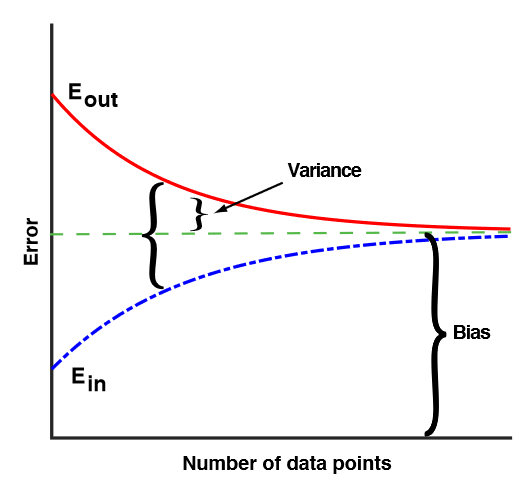
\includegraphics[width=0.7\linewidth]{bias-variance2.png}
		\caption[In-sample and out-of-sample error as function of training set size.]{Illustration of the in-sample error, $E_{\text{in}}$, out-of-sample error, $E_{\text{out}}$, variance, bias and difference of errors as function of the training set size. It is assumed that the number of data points is not small, and that we cannot exactly fit the true function $f(x)$. The training error increases while the test error decreases as the training set size increases. Figure is taken from ref. \citet{mehta2019high}. \label{fig:Bias-variance}}
	\end{figure} 
	
	
	\subsection{Bias-Variance Decomposition}
	\label{subsect:Theory-BiasVarianceDecomp}
	We will now go a bit further into the bias and variance that is an important aspect of machine learning. Lets consider a data set $\mathcal{D}(\textbf{X},\textbf{y})$ with $N$ pairs of independent and dependent variables. We then assume that the true data is created from a noise model 
	\begin{equation}
		y=f(x)+\epsilon,
	\end{equation}
	where $\epsilon$ is a normally distributed noise with mean zero and standard deviation $\sigma_{\epsilon}$. A chosen estimator $f(\textbf{x};\hat{\theta})$ is trained by minimizing the cost function, lets say the sum of squared errors\footnote{This is used in regression cases. For classification we could use cross-entropy for instance.}, 
	\begin{equation}
		\mathcal{C}(\textbf{y}, f(\textbf{X};\theta))=\sum_{i}(y_i-f(\textbf{x}_i;\theta))^2.
	\end{equation}
	
	Our best estimates for the model parameters,
	\begin{equation}
		\hat{\theta}_{\mathcal{D}}=\underset{\theta}{\argmin}\text{ } \{\mathcal{C}(\textbf{y},f(\textbf{X};\theta))\},
	\end{equation}
	are functions of the data set $\mathcal{D}$. Then we make another set of data sets $\mathcal{D}_n=(\textbf{y}_n,\textbf{X};n)$, where all sets have $N$ samples. We want the expectation value, $\mathds{E}_{\mathcal{D}}$, of the cost function of all these data sets. We also want the expectation value of the average over different noise instances $\mathds{E}_{\epsilon}$. The expected generalization error can be found to be (full derivation can be seen in Appendix \ref{appendix:BiasVarianceDecomp}):
	\begin{align}
	\label{eq:ExpctGenError}
		\mathds{E}_{\mathcal{D},\epsilon}[\mathcal{C}(\textbf{y}, f(\textbf{X};\hat{\theta}_{\mathcal{D}}))]&= \sum_i(f(\textbf{x}_i)-\mathds{E}_{\mathcal{D}}[f(\textbf{x}_i;\hat{\theta}_{\mathcal{D}})])^2 \nonumber\\
		& \quad +\sum_i \mathds{E}_{\mathcal{D}}[\{f(\textbf{x}_i;\hat{\theta}_{\mathcal{D}})-\mathds{E}[f(\textbf{x}_i;\hat{\theta}_{\mathcal{D}})]\}^2] 
		\nonumber\\
		& \quad + \sum_{i}\sigma_{\epsilon}^2
	\end{align}
	
	The first term in equation \ref{eq:ExpctGenError} is the bias
	\begin{equation}
	\label{eq:Bias}
		\text{Bias}^2=\sum_i (f(\textbf{x}_i)-\mathds{E}_{\mathcal{D}}[f(\textbf{x}_i;\hat{\theta}_{\mathcal{D}})])^2,
	\end{equation}
	and is a measure of the deviation of the expectation value of the model estimator from the true value. This is the best we can do in the infinity limit as we have already discussed. The second term is the variance 
	\begin{equation}
	\label{eq:Variance}
		\text{Var}= \sum_i \mathds{E}_{\mathcal{D}}[\{f(\textbf{x}_i;\hat{\theta}_{\mathcal{D}})-\mathds{E}[f(\textbf{x}_i;\hat{\theta}_{\mathcal{D}})]\}^2], 
	\end{equation}
	and measures the fluctuation in the estimator due to finite-sample effects. The last term is just a noise term $\text{Noise}=\sum_{i}\sigma_{\epsilon}^2$. By combining these three terms we can decompose the out-of-sample error as
	\begin{equation}
	\label{eq:OutOfSampleError}
		E_{\text{out}}=\text{Bias}^2+\text{Var}+\text{Noise}.
	\end{equation}
	It is often much simpler to train a very complex model than it is to obtain sufficient good data. Therefore it is normally more useful to use a less complex model with higher bias, since it is less sensitive to noise in the sampling data from having a finite-sized training data set.
	
	
	\subsection{Bias-Variance Tradeoff}
	\label{subsect:Theory-BiasVarianceTradeoff}
	Before we look into classification, we need to be aware of a few problems with supervised learning. First is the balance of variance and bias. This is called the \textbf{bias-variance tradeoff} in statistics and machine learning. We want to minimize both the variance and bias such that our model both works well on unseen data and captures the relations between the features and classes, but when one of them is lowered the other has a tendency to increase. High bias may lead to underfitting between the features and the classes, while high variance may lead to overfitting. When a model is overfit, it is excessively complex and will then model noise in the data as well. Overfit models will then do a great job during fitting, but worse on data outside of the training domain. Underfit models do not have the power to capture important variations in the data. With today's improved machinery, it is often easier to make a model too complex rather than to not.
	
	Second is the amount of training data that is available depending on the real function. For a more simple real function, the model does not need that much training data to learn on. While for a more complex\footnote{When we talk about simple and complex real function, we mean the complexity of interactions between the features and the number of features we use to approximate the true function.} real function, the model needs a lot of training data. 
	
	Third is the dimensionality of the features. If there are a lot of features with high dimensionality, the model may be confused and cannot separate out the most important features that defines the output. One way to fix this is to manually remove irrelevant features in the data that can confuse the model. The method for doing this is called \textbf{dimensionality reduction}, and there are several strategies for doing this. 
	
	The fourth and final major concern is noise or incorrect values in the desired output values. This often comes from human error or errors in sensors which can lead to overfitting. This can be fixed by e.g., remove noise training data or use early stopping. There also exists other factors that one need to consider, but these four bias-variance related issues are some of the biggest.
	
	In Figure \ref{fig:BiasVar} we see illustrations of the bias-variance tradeoff for training error, $E_{\text{in}}$, and test error, $E_{\text{out}}$, as the model complexity increases. In Figure \ref{subfig:BiasVar_a} we see that as the model complexity increases, the model fits the training data well leading to high variance. For a low complexity model the bias is high. This is exactly as we have already look at above. So we want a model that has a compromise between the variance and the bias, as seen by the optimal line in Figure \ref{subfig:BiasVar_a}. This optimal line is also where we have a minimum in $E_{\text{out}}$. For the prediction error for test and training samples in Figure \ref{subfig:BiasVar_b} as function of the model complexity, we see the variance and bias areas for low and high model complexities. From the gap between the two prediction error samples we see the same argument for choosing a optimal compromise between variance and bias. This will lead to a predicted error difference between training and test samples that is not to0 big and not to0 similar to each other. Often we want to use a more biased model with small variance to minimize $E_{\text{out}}$ and maximize the predictions.
	\begin{figure}[h!]
		\hspace*{-1.0cm}
		\subfloat[\label{subfig:BiasVar_a}]{\centering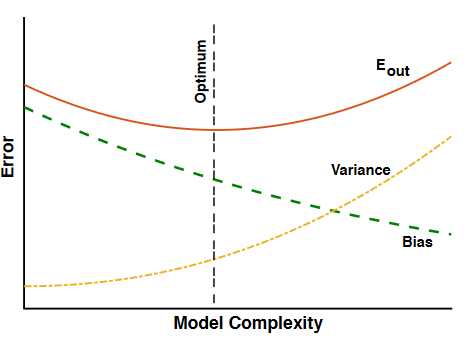
\includegraphics[width=0.55\linewidth]{bias-variance1.png}}
		%\hspace*{2.5cm}
		\hspace{0.45em}
		\subfloat[\label{subfig:BiasVar_b}]{\centering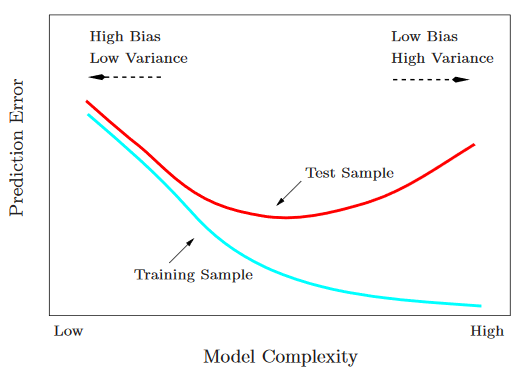
\includegraphics[width=0.55\linewidth]{bias-variance.png}}
		\caption[Bias-variance tradeoff and model complexity.]{Illustrations of the bias-variance tradeoff as function of model complexity. From these two illustrations we see that we want to find the optimal compromise between variance and bias that gives the best model, which does not underfit nor overfit the data. Figures are taken from ref. \citet{hastie2009elements} and \citet{mehta2019high}. \label{fig:BiasVar}}
	\end{figure}


	\subsection{Regularization}
	\label{subsect:Theory-Regularization}
	With increasing data power and amount of data collected, the data sets we can gather can be quite complex. This means that we need better machine learning models. With these better models we can solve more complex problems than before. As we mentioned earlier, this also gives rise to more problems, especially overfitting models. Overfitting is a more common issue than underfitting, since overfitting comes from models fitting functions and training data too well, making it perform worse on unseen (test) data. This is not something we desire to get, since machine learning is all about training model to analyze new data.
	
	Finding good methods to reduce overfitting has been an important aspect in machine learning a long time. That is the reason for developing \textit{regularization} techniques that reduces overfitting problems without significantly worsen the performance on the training data. Regularization techniques try to improve the generalization error of the test set. There are several different regularization methods that can be used, depending on the type of models which are used.
	
	One way is to tune the model complexity to be better at predicting. This is done by introducing a penalty for individual weights, $w$ . There are two types of norms of regularization that is often used; L1 and L2:
	\begin{align}
	\label{eq:L1Reg}
		L_{1,\text{norm}}&=\sum_{i}|w_i|\\
	\label{eq:L2Reg}
		L_{2,\text{norm}}&=\sum_{i}||w_i||^2
	\end{align}
	The L1 penalty will yield sparse feature vectors from the fact that most features weights will be zero. That means that the L1 norm can be seen as a kind of feature selection that removes irrelevant features in data sets with higher dimensionality that would only confuse the model when training. This feature reduction can also be done manually by removing the irrelevant features that makes the model underperform, making it less complex. The L2 norm also acts on the weights of the loss function. These two regularization norms are set in the models as \textit{hyperparameters}.
	
	Other ways to avoid overfitting is to \textit{prune} the models which use \textit{trees}\footnote{We will come back to what this is later.}, affecting the splitting of trees. \textit{Sampling} and \textit{early stopping} are other ways to control overfitting, by making boosted trees less correlated or stop training when a chosen training metric of a model no longer improves. All these ways to control overfitting are controlled by various input parameters numerically.
	
	
	\subsection{Hyperparameters}
	\label{subsect:Theory-Hyperparameters}
	As we have already mentioned, hyperparameters are something which need to be manually chosen before fitting a model. Hyperparameters help to tune and optimize the models in order to do a better fit of the data, and used to control the algorithms. These hyperparameters have no strict solution and change depending on the data set we are looking at. The same type of parameter may not have the same value in different models. For a small set of hyperparameters we could simply use trial and error to test the parameters. Most modern models require a lot of different hyperparameters. When there are a lot of parameters to tune, we may want to use some learning algorithm that searches through some given sets of hyperparameter values. An efficient method for doing this is to do a random search that uses the fact that not all hyperparameters are equally important. Searching for parameters are often computationally expensive since they require that the model is re-trained each time we change a configuration of hyperparameters.
	
	During the hyperparameter optimization, we want the test set to be isolated until the model is fully optimized. This is where the validation set becomes useful. The purpose of the validation set is to be used when training the model and optimize the hyperparameters. The first split of the original data set is into training and test sets. The training set can be further split into a smaller training set and a validation set. This means that we loose some training data which we need to take into consideration. The evaluation of the validation set will not be the exact same as evaluating the test set. The generalization error of the test set will be underestimated by the validation set error since the hyperparameters are trained on the validation set.
	
	
	\section{Classification}
	\label{sect:Theory-Classification}
	Classification is one of the most used and successful tasks in machine learning. Classification uses algorithms to decide which category the input belongs to. The function that produces an output value can be used to produce a probability distribution over the different outcomes. The simplest and probably most common classification problems are binary outcomes like True or False, Yes or No, Cat or Dog etc, where the outcomes are either the one or the other. When there are more than two outcomes, or classes, we use multiclass classification algorithms. Not all classification algorithms are made to classify instances with more than two outcomes, and cannot be used to classify problems other than binary outcomes. On the other hand, they can be turned into multiclassifiers by using various strategies. There are also other types of classifiers that are similar to multiclass classifiers, like multilabel and multioutput classification. They are similar, but are used in different cases with different outcomes. For example, multiclass classification labels a sample as one class only, meaning that it cannot be classified with two classes. This means that an image of a cat can only be classified as either a "cat" or a "dog" by the algorithm. The other two may categorize the image as both a "cat" and as "small" for instance.
	
	In this thesis, we use multiclass classification to classify different particles in event decay chains produced by colliding protons at the \acrshort{lhc}. In this thesis we will test different classification models and algorithms with various values for the hyperparameters for the respective models, to try and optimize and find the most accurate model. We will also study various evaluation metrics used to both find and evaluate the performance of the best model.
	
	
	\section{Classification Models}
	\label{sect:Theory-ClassModels}
	 A so-called "hard" classifier will assign each datapoint to a category, while a "soft" classifier will give the probability of a given category. The simplest classification algorithm is the "perceptron". It is given by the same transformation as linear regression with a weight matrix \textbf{w},
	 \begin{equation}
	 \label{eq:Perceptron}
	 	\textbf{y}=\textbf{X}\textbf{w}.
	 \end{equation}	 
	 The classes are then determined by the sign of the predictions by using sign functions or boundary thresholds. The perceptron is an example of a "hard" classifier. Sometimes it may be useful to use a "soft" classifier yielding category probabilities instead. 
	 
	 There are a lot of different classification models in machine learning with their own strengths and weaknesses. This is why we in this thesis will test a few different approaches and algorithms to find the best model for the analysis. In this section, we will briefly look at the classification methods we will test in this thesis.
	
	
	\subsection{Logistic Regression}
	\label{subsect:Theory-LogisticRegression}
	A simple "soft" model in statistical analysis for classifying discrete outcomes is logistic regression (\acrshort{lr})\cite{mehta2019high}. It uses linear regression to fit data and a logistic function\footnote{It can also be called an activation function.}, usually the Sigmoid function 
	\begin{equation}
	\label{eq:Sigmoid}
		\sigma(s) = \frac{1}{1+e^{-s}},
	\end{equation}
	to predict the outcomes into categories using probabilities. A threshold for the predicted values is chosen which determines which classes the data belongs to. These boundary thresholds can be complex and doesn't have to be linear. The cost function is the usually cross-entropy with added $L_1$ (eq.\ref{eq:L1Reg}) and $L_2$ (eq.\ref{eq:L2Reg}) regularization terms. The cross-entropy is the negative log-likelihood of the prediction being in the data set. The cross-entropy is derived from the fact that the Maximum Likelihood Estimator (\acrshort{mle}) is the set of parameters that maximize the log-likelihood.
	
	The most basic model is a Binary Logistic Regression that yields two possible outcomes. However, it can be extended to more than two outcomes by using Multinomial Logistic Regression (\acrshort{mlr}. Both \acrshort{lr} and \acrshort{mlr} can be combined with cross-validation, using various optimization solvers supporting the regularization parameters as input.
	
	
	\subsection{Multi-Layer Perceptron}
	\label{subsect:Theory-MLP}
	A Multi-Layer Perceptron (\acrshort{mlp})\cite{MLP} is an artificial feed-forward neural network (\acrshort{ffnn}) model consisting of interconnected nodes, and is similar to \acrshort{lr} in that it has an \textit{input} and an \textit{output layer}, but differs in that between these layers, the \acrshort{mlp} can have several non-linear layers called \textit{hidden layers}. In a \acrshort{ffnn} the information only goes one way. The inputs are called neurons and are transformed in the hidden layers by a weighted linear summation of the inputs and a non-linear activation function to determine the outputs for each layer. The hidden layers often have some bias to ensure non-zero values. The output layer transforms the values from the last hidden layer into output values. In Figure \ref{fig:MLP}a we see how each node in a neural network is connected to all the nodes in the previous layer with a weight value. Then it goes to a non-linear activation function that transforms the node to an output either to a new node in a hidden layer or to the output layer. The nodes will have some bias term individually connected to them. In Figure \ref{fig:MLP}b we see a fully connected neural network since all nodes are connected to all nodes in the next layer.
	\begin{figure}[ht!]
		\hspace*{-1.0cm}
		\centering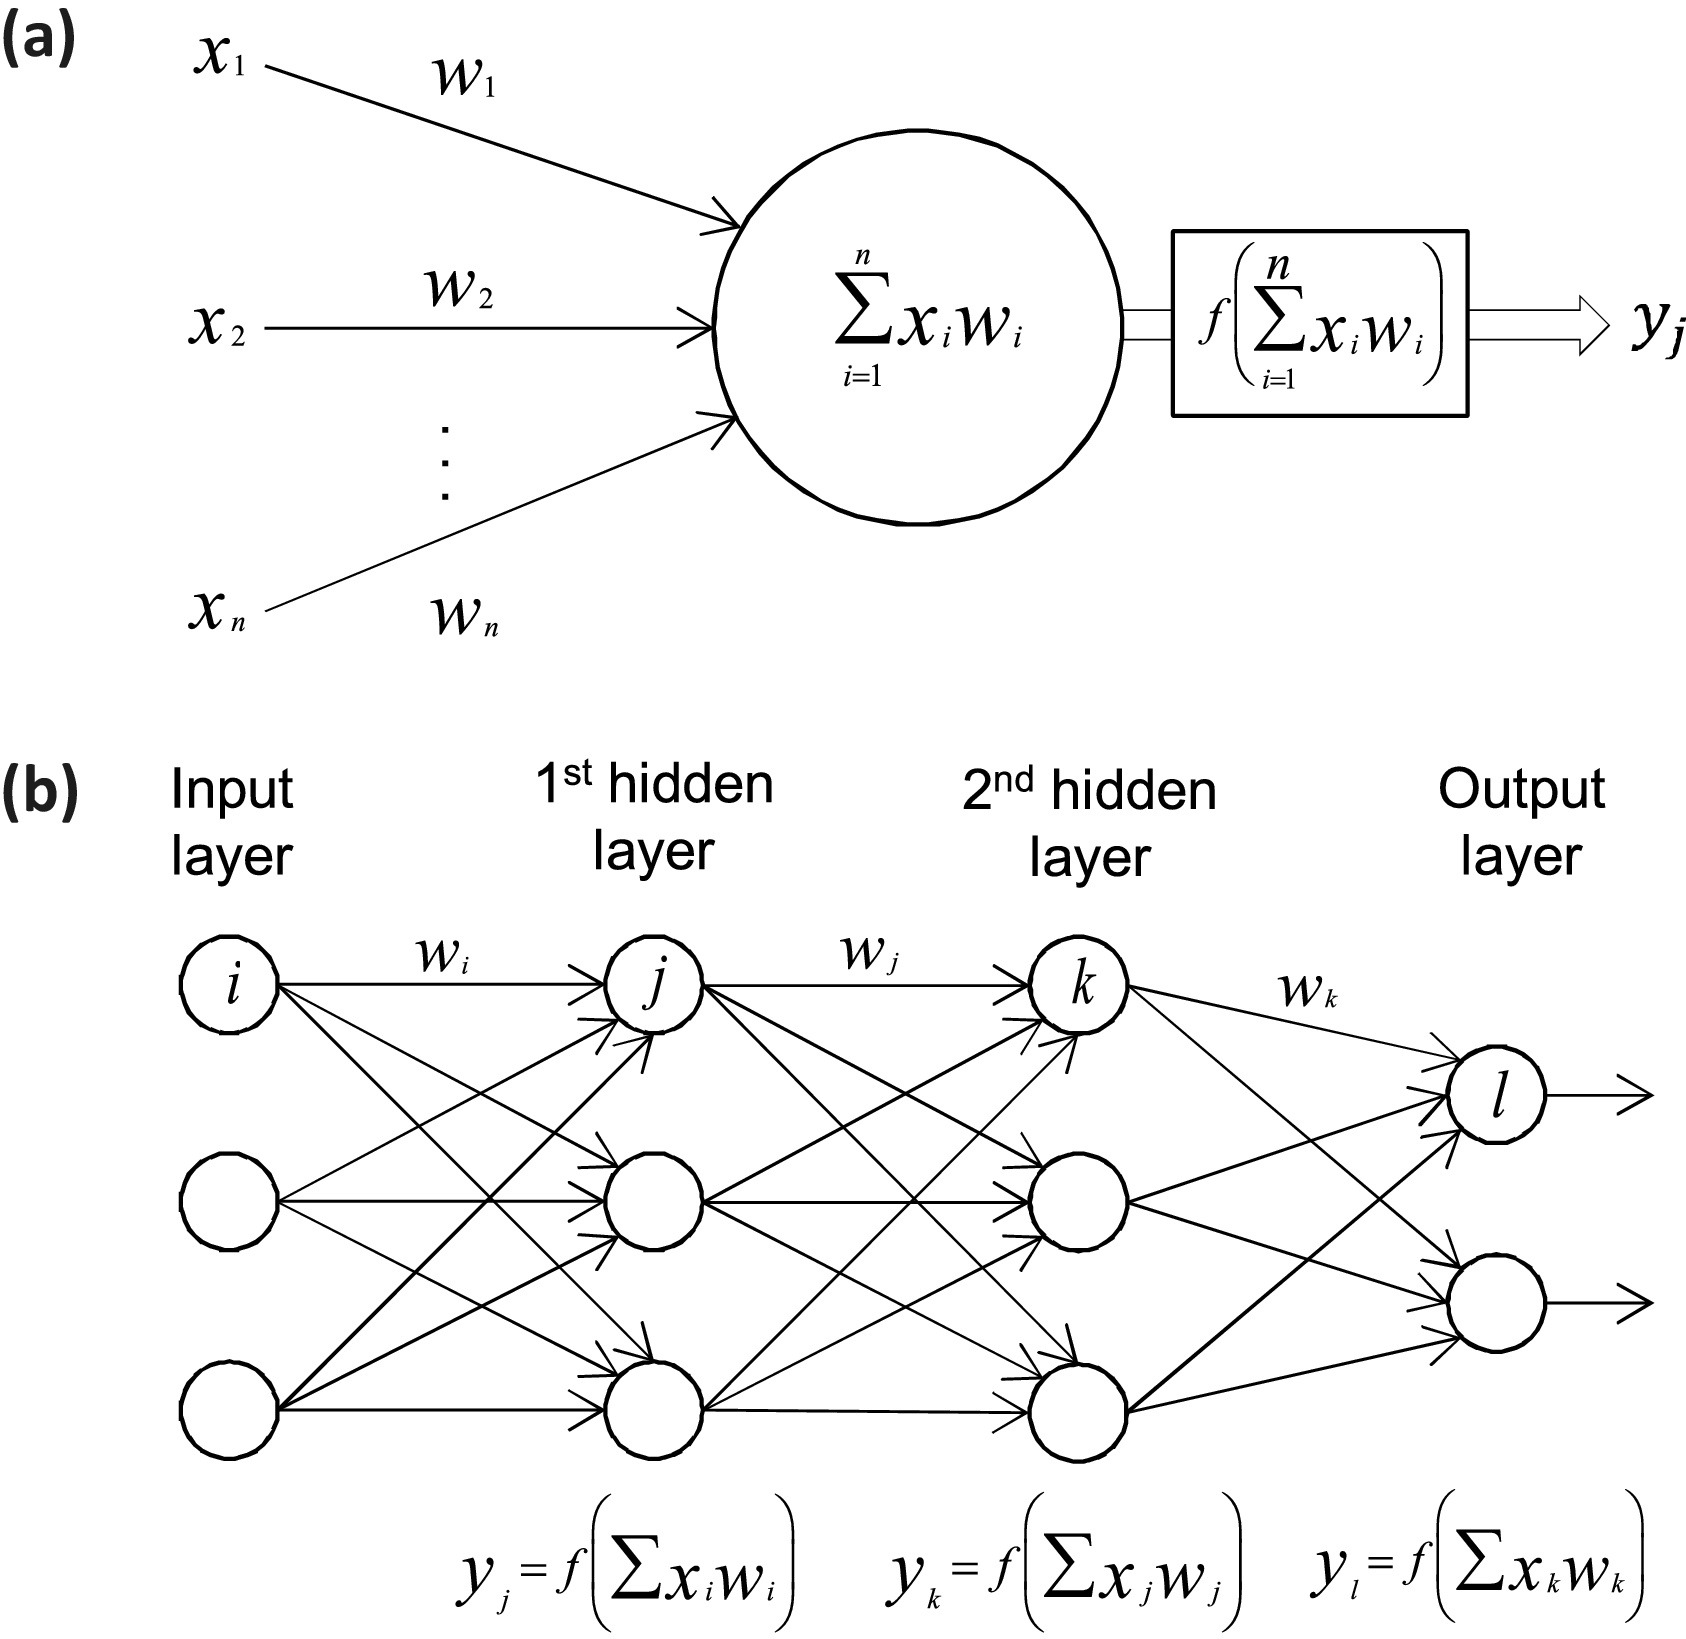
\includegraphics[width=0.7\linewidth]{mlp.jpg}
		\caption[Multi-Layer Perceptron illustration.]{(a) Each node in a neural network has some input acted on by some associated weights. Then the weighted inputs are summed together inside the node and passed to a non-linear activation function which transforms it to an output. (b) This is a \acrshort{ffnn}/\acrshort{mlp} with 3 inputs, 2 hidden layers and 2 classes. All the nodes in one layer is connected to all the nodes in the next layer. This is then a fully connected neural network. Figure is taken from ref. \citet{MLP_network}. \label{fig:MLP}}
	\end{figure}
	
	The \acrshort{mlp} trains the model using \textit{backpropagation} with initial guesses for the biases and weights. Backpropagation is a method used to optimize the weights and biases to minimize he cost function. The backpropagation iterates backwards from the last layer to the first layer using gradient descent of the weights and biases to start a new feed-forward process from the input layer. This process is repeated until the cost function is sufficiently minimized. 
	
	Typical choices of activation functions are the hyperbolic tangent function, the sigmoid and the rectified linear unit function (\acrshort{relu}). The choice of cost function also needs to be considered. The \acrshort{mlp} library in \textit{Scikit-Learn} only supports the cross-entropy loss function as the cost function.
	
	Neural networks typically have a large amount of parameters which often leads to overfitting. That is why we add a $L_2$ regularization penalty to the weights. This hyperparameter have to be tuned. Another hyperparameter that is needed is the \textit{learning rate}. This parameter is used to control the step length in the optimization of the cost function with a gradient descent method. In neural networks the weights and biases are the parameters to be adjusted, while it can be different in other models. There are several gradient descent methods, e.g. the stochastic gradient descent with minibathces, which can be used to avoid interpreting a local minimum as a global minimum. A more modern method is the \textit{adam} solver proposed by \citet{adam}. It is a stochastic gradient-based optimizer which combines an adaptive learning rate\footnote{It adjusts the learning rate as it iterates towards the minimum.} with other functions, and thus adds a few more hyperparameters to be tuned, i.e. $\beta_1$, $\beta_2$ and $\epsilon$.
	
	For multiclass classification, the softmax function is used as the last hidden layer activation function. It normalizes the output of the network into a probability distribution over the predicted output classes.
	
	
	\subsection{Decision Tree}
	\label{subsect:Theory-DecisionTree}
	Decision Trees (\acrshort{dt}s)\cite{DecisionTree} tries to learn simple decision rules from the data features by constructing tree-like models to predict the target values. The models simply break down a complex decision into several simpler decisions. Each tree starts of with a single \textit{root} node containing all the class labels. The root node then splits into several smaller \textit{internal} nodes, which then splits into \textit{leaf} nodes in the end representing the class targets. The splits are decided by some chosen \textit{criterion} function that uses a certain strategy to do the splits. The root node is chosen as the feature with the highest information gain value by the criterion function. The path from the root node to an internal node or a leaf is always unique, and the leaves do not have any descendants.
	
	The \acrshort{dt} uses a cost function to determine the the most homogeneous branch when splitting. The stopping point for splitting is something we can set as an input parameter to the model by choosing a maximum depth of the tree from the root to the leaves, or by setting the maximum number of leaves at the end. Other parameters for controlling the size and splitting of the tree should be considered since the \acrshort{dt} is prone to overfitting with many features. This can be fixed by pruning the tree, i.e. to remove nodes with low importance features, use dimensionality reduction with e.g. principal component analysis (\acrshort{pca})\cite{PCA} or decrease some of the controlling parameters.
	
	There are a few different \acrshort{dt} algorithms to generate the optimal trees. The algorithm that is implemented in Scikit-Learn is an optimized version of the Classification and Regression Trees (\acrshort{cart}) algorithm that construct binary trees from the features and thresholds for giving the highest information gain at each node. The Scikit-Learn \acrshort{dt} classifier automatically supports multiclass classification.
	
	
	\subsection{Random Forest}
	\label{subsect:Theory-RandomForest}
	Another classification ensemble method is the Random Forest (\acrshort{rnf})\cite{randomforest} algorithm. It produces a number of \acrshort{dt} classifiers on bootstrapped training samples with a low correlation to each other, and uses their average like the bagging method. This improves the accuracy score and helps control overfitting. One can also choose to bootstrap samples. 
	
	Like with the \acrshort{dt} algorithm, we can control the size and splitting of the tree. The \acrshort{dt} and \acrshort{rnf} algorithms are very similar and have many of the same input parameters and same procedure for building the trees. The main difference is that with the \acrshort{rnf} algorithm, we produce many trees with sources of randomness. This randomness is very important in that it decreases the variance when combining and taking the average of many trees, and can cancel out some prediction errors. This normally yields a better model.
	
	
	\subsection{AdaBoost}
	\label{subsect:Theory-AdaBoost}
	Instead of using average ensembles where we use many independent bootstrap samples, we can use something called \textit{boosting}. This is a type of method which keeps the weight for each iteration, and the base estimators are built sequentially. The boosting model then builds a combined estimator that reduces the bias and the variance. The result is to get a powerful ensemble from several weaker models combined.
	
	One such boosting method is the AdaBoost classifier\cite{bagging}\cite{AdaBoost}. The AdaBoost uses adaptive boosting and weaker classifiers as estimators to sequentially combine them into a single better classifier with a weighted majority. It will fit weaker classifiers sequentially such that the next classifier will have a different weight than the previous to adjust for incorrect classification in the previous. Data which are difficult to predict will then have an increasing influence since the next classifier will learn from the mistakes of the previous weaker classifier. The final prediction is the result of a weighted majority vote of the combination of the weaker classifier predictions. A weaker classifier can then be boosted to a stronger classifier that is more accurate.
	
	The AdaBoost algorithm in Scikit-Learn takes a weaker classification algorithm as input together with the maximum number of estimators to be boosted before stopping. If the model is to be perfectly fit, the executing will also be stopped. It also takes a learning rate parameter for the shrinking of the classifiers. The AdaBoost algorithm can naturally detect and adapt to a multiclass problem.
	
	
	\subsection{Gradient Boosting}
	\label{subsect:Theory-GradientBoost}
	Gradient Boosting Decision Tree (\acrshort{gbdt})\cite{GradientBoost} is another boosting method like AdaBoost. The \acrshort{gbdt} is an additive model that tries to identify the shortcomings of the weak classifiers. While AdaBoost uses high weight data points, the \acrshort{gbdt} uses the same for gradients in the loss function. This allows the cost function to become better for optimizing the fitting. The $K$ number of regression trees\footnote{For a binary classification case, only a single tree is fit.} at each stage are fit on the negative gradient of the binomial (binary class) or multinomial (multiclass) deviance loss function.
	
	The algorithm is well suited for both binary and multiclass classification, and takes the maximum number of estimators and the learning rate as input parameters. Since it is a boosted tree method, it can also take the maximum depth of the trees and maximum number of leaves as inputs. It is also quite robust against overfitting. In a multiclass problem, the algorithm will create $K$ trees for each iteration when we have $K$ classes. The loss function for multiclass also have to be "deviance" to give probabilistic outputs (similar to \acrshort{lr}).
	
	When dealing with larger data sets (n\_samples$>$10 000) or a large number of classes, a histogram-based gradient estimator can be more useful. Scikit-learn has an experimental implementation of \acrshort{gbdt}s called \textbf{HistGradientBoostingClassifier} which is inspired by \citet{lightgbm} on a \textbf{LightGBM} algorithm. This estimator can be orders of magnitude faster than the original \acrshort{gbdt} estimator. To reduce the computation time and number of splitting points, the algorithm bins the input samples into integer-valued bins. They share most of the same parameter inputs which controls the models, except that the histogram-based estimator gets a parameter for controlling the number of bins. This can act as another regularization parameter. 
	
	
	\subsection{Extreme Gradient Boosting}
	\label{subsect:Theory-XGB}
	Another highly efficient, flexible and portable tree boosting method is the Extreme Gradient Boosting (\acrshort{xgb})\cite{xgboost}. It is a scalable end-to-end tree boosting system using an optimized distributed gradient boosting algorithm and provides fast and accurate parallel tree boosting. It is one of the most used and highly recognized machine learning algorithms today together with deep neural networks. The \acrshort{xgb} algorithm won the Kaggle Higgs ML challenge in 2014\cite{MLHiggs}. One of the most important aspects of the \acrshort{xgb} is its scalability, making it several times faster than other algorithms combined with parallelization. 
	
	The \acrshort{xgb} algorithm uses the \acrshort{gbdt} framework as its core. It looks at distributions of the features for all data points in a leaf to build trees using potential loss for the possible splits to make a new branch. This decreases the space of possible feature splits search. The algorithm chooses features and split-points based on the criteria to maximize the gain. The splits are binary such that it splits according to if a value is bigger or lower than a threshold set by the algorithm. The gain is different depending on the type of loss function which is used. With a small data set, the \acrshort{xgb} algorithm tries all split points gained by the data values for each feature. The feature and threshold combination with the highest gain is then chosen. For a larger data set, the algorithm uses fewer candidate splits given by the quantiles of the data. 
	
	Since \acrshort{xgb} is more complex than other algorithms, it also requires more parameters to be tuned to control the model properly. The parameters can be sorted into \textit{general parameters} for choosing the booster method, \textit{booster parameters} which are dependent on the boosting method and \textit{task parameters} which specify learning task parameters and learning objectives. We are using a tree booster which has many of the same tree boosting parameters as the \acrshort{dt} and \acrshort{rnf} algorithms, i.e. regularization terms, hyperparameters for tree controlling, pruning and others. The task parameters include the type and size of the classes we have, e.g. multiclass classification, and types of evaluation metrics to use.
	
	
	\subsection{Light Gradient Boosting Machine}
	\label{subsect:Theory-LGBM}
	Light Gradient Boosting Machine (\acrshort{lgbm})\cite{lightgbm} is a distributed gradient boosting framework for machine learning. It is similar to the \acrshort{xgb} algorithm, but made to be faster, around 7 times faster, with higher efficiency, lower memory usage and better accuracy. This is a huge advantage when dealing with larger data sets. The \acrshort{lgbm} algorithm uses a gradient based one-side sampling and exclusive feature bundling for filtering the data samples to find the split value in the trees, while the \acrshort{xgb} uses a histogram based algorithm to find the best splits. This means that the \acrshort{lgbm} algorithm will keep features with higher absolute values, regarding information gain, than a pre-defined threshold and drop the features with small absolute values. This will improve the accuracy. The features that rarely have non-zero values simultaneously will be combined into a single feature, to reduce the number of features in the data set. \acrshort{xgb} and \acrshort{lgbm} have very similar input parameters.
	
	
	\subsection{Multiclass Classification Models}
	\label{subsect:Theory-MultiClassModels}
	To do multiclass classification, there are several existing techniques. We will look more into two of those techniques\footnote{There is also a third technique, hierarchical classification, that we will not cover.}; transformation to binary and extension from binary. These are all meta-estimators. This means that they all need a base estimator, most often a binary classifier, which is extended to do multiclass classification when they are implemented in the constructors.
	
	The extension from binary technique is rather trivial. We simply use already existing binary classifiers and modify them to do multiclass classification. Not all binary classifiers can be extended to multiple classes. The classification models we have looked at, this far, can either do this automatically, or have input parameters and constraints in the models to tell the models to do multiclass classification.
	
	Transformation to binary reduces our multiclass problem down to several binary classification problems. This technique can also be split into more strategies, which we will look more into.  
	
	
	\subsubsection{One-Vs-Rest Classifier}
	\label{subsubsect:Theory-OvRModel}
	The first strategy is the one-vs-rest (\acrshort{ovr}) classifier. Each class in this model has its own classifier which does the fitting, and the classifier fits the single class against the rest of the classes. This means we only need $n$ classifiers for the $n$ classes. This also improves interpretability, since we can get information about a specific class by looking at its classifier.
	
	The \acrshort{ovr} takes a input a binary classifier along with samples and targets and outputs a list of the classifiers for each class. When doing predictions, it uses all the classifiers on unseen data and picks the class with the highest confidence score.

	
	\subsubsection{One-Vs-One Classifier}
	\label{subsubsect:Theory-OvOModel}
	The second strategy is the one-vs-one (\acrshort{ovo}) classifier. This takes one classifier and a pair of classes at a time. For each pair of classes, the classifier trains on data containing these classes and learns to distinguish them. This happens between all the classes. It then uses a voting scheme to select the class with the most votes. For $n$ number of classes in the multiclass problem, the \acrshort{ovo} trains $n(n-1)/2$ binary classifiers. All the classifiers that are trained will be applied when doing the prediction on unseen data, and the one with the highest number of predictions will be predicted by the combination of classifiers.
	
	This method is slower than the \acrshort{ovr} since it has a $\mathcal{O}(n^2)$ complexity. Both the \acrshort{ovo} and \acrshort{ovr} methods suffer from the fact that there may be regions where the input space can get the same number of votes.
	
	
	\section{Evaluation Metrics}
	\label{sect:Theory-EvalMetrics}
	To evaluate the performance of the classification models properly and decide which model best fits the data, we need to have some evaluation metrics. In this section we will take a look at the evaluation metrics used for the classification\footnote{See Scikit-Learn\cite{scikit-learn} for more details on metrics.}. 
	
	
	\subsection{Mutual Information}
	\label{subsect:Theory-MutualInfo}
	To look closer at the correlations in the data set, we can use the entropy and information gain. The entropy can be calculated using the probability $P(j)$ of a value $j$ occurring, where $j$ is a value which a feature group $x_i$ can take;
	\begin{equation}
	\label{eq:Entropy}
		H(x_i) = -\sum_{j\in x_i}P(j)\log_2 P(j)
	\end{equation}
	With a given target \textbf{y}, we can calculate the conditional entropy of a feature $x_i$:
	\begin{equation}
	\label{eq:CondEntropy}
		H(x_i|\textbf{y})=-\sum_{y\in \textbf{y}}P(y)\sum_{j\in x_i}P(j|y)\log_2 P(j|y)
	\end{equation}
	Now we compute the information gain, or \textit{mutual information} in the context of variable selection, for a given feature as the difference between these two entropies:
	\begin{equation}
	\label{eq:InfoGain}
		I(x_i:\textbf{y})=H(x_i)-H(x_i|\textbf{y})
	\end{equation}
	With the information gain we get a measure of the correlation between a feature and the target, which shows dependencies between features and the amount of information that one feature provides about others.
	

	\subsection{Accuracy Score}
	\label{subsect:Theory-Accuracy}
	To measure the performance of the models, we use the the accuracy score for classification. This is a measure on how well the models can predict the classes. It is defined as the number of correct predictions divided by the total number of predictions, giving a value between 0 and 1. 
	\begin{equation}
	\label{eq:AccuracyScore}
		\text{Accuracy}=\frac{\sum_{i=1}^nI(\tilde{y}_i=y_i)}{n},
	\end{equation}
	where $\tilde{y}_i$ is the predicted target by the model, $y_i$ is the actual class target, $n$ is the total number of predictions and $I$ is and indicator function
	\begin{equation}
	\label{eq:IndicatorFunc}
		I = \begin{cases*}
			1, \text{ if $\tilde{y}_i=y_i$ }\\
			0, \text{ if $\tilde{y}_i\neq y_i$}
			\end{cases*}
	\end{equation}
	When the model prediction fits the data perfectly we get an optimal score of 1. 
	
	The accuracy score can be computed for all data sets, i.e. training validation and test sets. If there is a big difference between the accuracy score for either validation and training or test and training, we might under- or overfit the data. When the training score is much better, we most likely overfit the data.
	
	Another way to balance out the accuracy scores is to use \textit{cross-validation}. It's a very useful technique against overfitting, and can be used to tune hyperparameters. There are several cross-validation techniques, but the main idea of cross-validation is to divide samples into subsets. The cross-validation will do the analysis on one subset and compute the accuracy on that subset. Then it will do another analysis with another subset and compute the accuracy again. After many iterations, dividing the data into subsets and computing several accuracy scores, the average score is used as an estimate of the model performance. 
	
	
	\subsection{Cohen Kappa Score}
	\label{subsect:Theory-CKS}
	Another scoring statistic is the Cohen Kappa Score (\acrshort{cks})\cite{cks}. The \acrshort{cks} accounts for uncertainties in the predictions, comparing a random classifier against a more accurate and tuned classifier. The \acrshort{cks} is calculated by using the rate of agreement for random guessing, $p_e$, and the rate of agreement for the actual prediction, $p_a$. The \acrshort{cks} ranges from -1 to 1, where 1 is the optimal score representing perfect agreement, 0 represents agreement that can be expected by random guess and -1 represents no agreement, and is calculated as 
	\begin{equation}
	\label{eq:CohenKappa}
		\kappa=\frac{p_a-p_e}{1-p_e}
	\end{equation}
	
	
	\subsection{Error Evaluation}
	\label{subsect:Theory-ErrorEval}
	We will use several different error metrics to get a good overall error estimate of the classification models. These will also help to discover any over- or underfitting of the data.
	
	
	\subsubsection{Error Rate}
	\label{subsubsect:Theory-ErrorRate}
	With the accuracy score, we can compute the \textit{error rate}. The error rate is defined as the fraction of misclassifications:
	\begin{equation}
	\label{eq:error}
		\text{error} = 1 - \text{accuracy}
	\end{equation}
	This is an often used metric in classification. Both the error and the accuracy score can be computed in multiclass classification cases.
	
	
	\subsubsection{Log Loss}
	\label{subsubsect:Theory-LogLoss}
	Instead of using discrete predictions, we can evaluate probability outputs of classifiers. We can use the \textit{log loss} function, also called the cross-entropy or logistic regression loss, to evaluate the probabilities. When dealing with a binary case with a probability estimate $p=P(y=1)$, the log loss is defined as the negative log-likelihood given a true output for each sample. It is computed as
	\begin{equation}
	\label{eq:LogLossBin}
		L_{\text{log}} = -\log P(y|p)=-(y\log (p) + (1-y)\log(1-p)).
	\end{equation}
	
	For a multiclass case, the log loss is taken over a whole set of size $n$ with $K$ labels, a binary indicator matrix \textbf{Y} and a matrix \textbf{Pr} of probability estimates as
	\begin{equation}
	\label{eq:LogLossMulti}
		L_{\text{log}}(\textbf{Y},\textbf{Pr})=-\log P(\textbf{Y},\textbf{Pr})=-\frac{1}{n}\sum_{i=1}^{n}\sum_{k=1}^{K}y_{i,k}\log p_{i,k}.
	\end{equation}


	\subsubsection{Variance}
	\label{subsubsect:Theory-Variance}
	Previously in section \ref{subsect:Theory-BiasVarianceDecomp}, we defined the variance and the bias of a model. These two are used to check for possible under- and overfitting. The variance is a measure of how far the spread of our predictions are from their average values. Given the predictions, $\tilde{\textbf{y}}$, of a model, the variance is calculated as
	\begin{equation}
	\label{eq:VarianceClass}
		\text{Var}(\tilde{\textbf{y}})=\frac{1}{n}\sum_{i=1}^n(\tilde{y}_i-\frac{1}{n}\sum_{j=1}^n\tilde{y}_j)^2.
	\end{equation}

	
	\subsubsection{Bias}
	\label{subsubsect:Theory-Bias}
	The bias error is a measure of the difference between the true values, $\textbf{y}$, and the average of the predicted values. To get the out-of-sample error in equation \ref{eq:OutOfSampleError}. The bias squared can be calculated as
	\begin{equation}
	\label{eq:BiasClass}
		\text{Bias}^2(\textbf{y}, \tilde{\textbf{y}})=\frac{1}{n}\sum_{i=1}^n(y_i-\frac{1}{n}\sum_{j=1}^n\tilde{y}_j)^2.
	\end{equation}
	
	
	\subsection{Classification Report}
	\label{subsect:Theory-ClassReport}
	With Scikit-Learn, we can easily build what is called a \textit{classification report}. This is a text report containing some useful classification metrics using the true targets and predictions of the model.
	
	First we will look at some useful prediction results used to compute some of the report metrics:
	\begin{enumerate}
		\item Positive (P) - The observation is positive.
		\item Negative (N) - The observation is negative.
		\item True Positive (TP) - Observation is positive, and the prediction is positive.
		\item True Negative (TN) - Observation is negative, and the prediction is negative.
		\item False Positive (FP) - Observation is negative, but the prediction is positive.
		\item False Negative (FN) - Observation is positive, but the prediction is negative.
	\end{enumerate}
	With the last four outcomes above (3-6), we can compute some useful metrics in the report:
	\begin{enumerate}
		\item[] Precision - The fraction of a sample classified correctly as positive of all positive predicted samples by the model:
		\[\frac{TP}{TP+FP}\]
		\item[] Recall - The fraction of a sample classified correctly as positive of all positive observations (true positive rate):
		\[\frac{TP}{TP+FN}\]
		The recall of the positive class is also called the sensitivity. The recall of the negative class (true negative rate) is called the specificity.
		\item[] F1-score - A weighted average of the precision and recall:
		\[2\times\frac{\text{Precision}\times \text{Recall}}{\text{Precision}+ \text{Recall}}\]
	\end{enumerate}
	In the multiclass case, these metrics are computed for each class independently. 
	
	The classification report also includes for various classification cases:
	\begin{enumerate}
		\item[] Support - The number of true classes in the data set for each class.
		\item[] Accuracy - The accuracy score of the model (binary case).
		\item[] Macro avg - Average of the unweighted mean for each class.
		\item[] Micro avg - Average of the total true positives, false negatives and false positives (multiclass or multilabel cases).
		\item[] Weighted avg - Average of the support-weighted mean for each class.
		\item[] Sample avg - Average of samples (multilabel case).
	\end{enumerate}
	
	
	\subsection{Confusion Matrix}
	\label{subsect:Theory-ConfusionMat}
	With the four outcomes in the classification report (3-6), we compute a \textit{confusion matrix}. For a binary case, the confusion matrix looks like Figure \ref{fig:ConfusionMatrix}. Here we see the predictions versus the true values. It gives a better understanding of the accuracy of a classification model. The accuracy score shows the overall accuracy, whereas the confusion matrix shows the predictions and accuracy of each class. It is easily extended for multiclass classification as a matrix with dimension $k\times k$ for $k$ classes. When the confusion matrix is normalized the total values of the rows are equal to 1. In the optimal case with all predictions correctly guessed, we should have 1's along the diagonal and 0 elsewhere.
	\begin{figure}[htb!]
		\hspace*{-1.0cm}
		\centering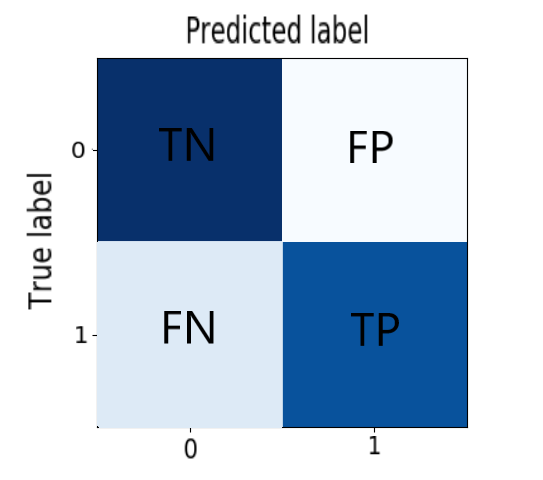
\includegraphics[width=0.6\linewidth]{Conf_mat.png}
		\caption[Confusion matrix.]{The confusion matrix is used to evaluate the accuracy of a classification model by using the four true and false observation and prediction outcomes (TP, TN, FP, FN. See sect. \ref{subsect:Theory-ClassReport}.). \label{fig:ConfusionMatrix}}
	\end{figure}


	\subsection{Precision-Recall Curve}
	\label{subsect:Theory-PrecisionRecall}
	Scikit-Learn provides a useful function for plotting precision versus recall. In Figure \ref{fig:PrecisionRecall} we see an example of how a precision-recall curve can look like in a multiclass case with 10 classes. This lets us see how the precision and recall behaves for different thresholds. A large \acrshort{auc} is the result of both high precision and high recall, which is preferable. The range of values will be between 0 and 1, as for accuracy. When the area under the curve (\acrshort{auc}) of a class is close to 1, the classification model can predict this class with a good accuracy. For a multiclass-case, the precision and recall are computed for each class as binary cases. A large area for each class is the optimal case here as well.
	\begin{figure}[htb!]
		\hspace*{-1.0cm}
		\centering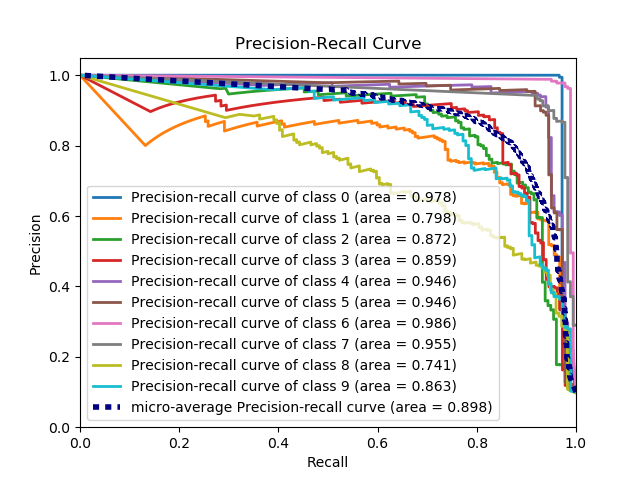
\includegraphics[width=1.0\linewidth]{precision_recall_curve.png}
		\caption[Precision-Recall Curve.]{Example of a precision-recall curve for a multiclass classification case with 10 classes and a micro-average curve plotted. Most of the classes have a large \acrshort{auc}, showing that the classifier can predict these classes with good accuracy. Credits Scikit-Learn \cite{scikit-learn}. \label{fig:PrecisionRecall}}
	\end{figure}
	
	
	\subsection{Balanced Accuracy}
	\label{subsect:Theory-BalancedAcc}
	If we are dealing with imbalanced data sets, we can use \textit{balanced accuracy}. It uses a macro-average of the recall for each class. When we have a balanced data set, this just becomes the standard classification accuracy. It is computed as the mean of the sensitivity and the specificity:
	\begin{equation}
	\label{eq:BalancedAcc}
		\text{Balanced-accuracy}=\frac{1}{2}\left(\frac{TP}{TP+FN}+\frac{TN}{TN+FP}\right)
	\end{equation}
	The balanced accuracy ranges from 0 to 1.
		
	
	\subsection{ROC Curve}
	\label{subsect:Theory-ROC}
	The Receiver Operating Characteristic (\acrshort{roc}) curve utilizes the \acrshort{auc} to summarize the overall performance of classification models. An example of a \acrshort{roc} curve plot can be seen in Figure \ref{fig:ROC} with a multiclass case with 10 classes. This results in 10 \acrshort{roc} curves, a random model curve and two different average curves, as seen in the figure. The \acrshort{roc} curve function in Scikit-Learn plots the sensitivity versus the specificity for a model. A totally random model would result in an \acrshort{auc} of 0.5, showing as the straight dashed line from the left bottom corner to the right top corner in the figure. The optimal model would show an infinitely quick incline in the \acrshort{roc} curve at the beginning, before flattening out with \acrshort{auc} close to 1. A good classifier would typically have an \acrshort{auc} larger than 0.8.
	\begin{figure}[htb!]
		\hspace*{-1.0cm}
		\centering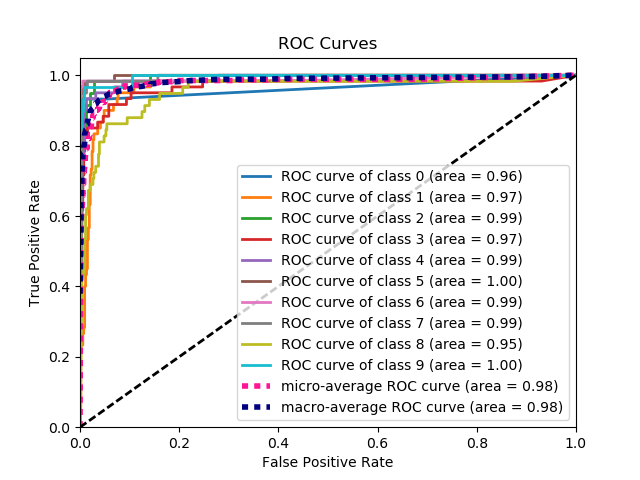
\includegraphics[width=1.0\linewidth]{roc_curve.png}
		\caption[ROC Curve.]{Example of a \acrshort{roc} curve for a multiclass classification case with 10 classes, a micro-average curve, a macro-average curve and a random model (black dashed line) plotted. All classes and averages have large areas under the curves, showing that the classifier can predict the classes with good accuracy. Credits Scikit-Learn \cite{scikit-learn}. \label{fig:ROC}}
	\end{figure}
	

%----------------------------------------------------------------------
%----------------------------------------------------------------------

	\part{Implementation}
	\label{part:Implementation}
	
	\chapter{Preparing for Machine Learning}
	\label{chap:Method-Methods}
	In this part we will look at the framework of the classification exploiting a range of different models. First we will look at the data and how it is made and converted to fit our purposes. The data is already produced beforehand as ROOT files (more in sect. \ref{sect:Method-Data}) and will be converted into data frames with Python where we will make new features as well as the target values. The data will then be analyzed and preprocessed (sect. \ref{sect:Method-PrepData}) with different methods before it is split into training, validation and test sets. We will then go through some of the tuning which is done with the models on the validation set using the evaluation metrics from section \ref{sect:Theory-EvalMetrics}, before we apply the best fit model on unseen data. The best model will be used to classify the vertices of the leptons in background and signal data. The results will be presented in part \ref{part:Results} and discussed in part \ref{part:Conclusion}.
	
	Python is used for easy implementation of machine learning libraries with Scikit-Learn and for plotting, using the Matplotlib library. In the following section, we will give a brief presentation of the most important Python libraries we use in our code.
	
	
	\section{Python Libraries}
	\label{sect:Method-Packages}
	Many of the libraries we use require other libraries to be installed, but they do not have to be explicitly imported in the code itself. The code and necessary software requirements are found in the GitHub repository\footnote{https://github.com/krilangs/ComPhys---Master}. It contains explanations on how to setup and run the code.
	
	When we present code snippets in this thesis, we will leave out some parts, noted by "$\backslash\backslash$...", since it will only be used for visualization of the code. The full source codes can be found in the GitHub repository. 
	
	\begin{itemize}
		\item \textbf{NumPy}: NumPy, or Numerical Python, is one of the most used packages in Python. It handles arrays, matrices, has functions for working with high-level mathematics, can dump data to files and more.
		\item \textbf{Pandas}: Pandas is a powerful and easy Python made library for handling data manipulation and analysis. This library is very useful with machine learning for handling the data for visualization, since it creates data structures that are flexible, efficient, customizable and easy to use and read.
		\item \textbf{Matplotlib}: Matplotlib is a plotting library for Python and NumPy which creates graphs and visualizations.
		\item \textbf{Seaborn}: Seaborn is a more high-level visualization library, and is based upon Matplotlib. It is most used for statistical graphics to understand data better, and is closely connected to pandas. 
		\item \textbf{ROOT}: ROOT, or PyROOT, is ROOT's Python C++ bindings. It lets us use ROOT in Python. This is very much used in particle physics. This also lets us use Python libraries like NumPy and Pandas combined with ROOT.
		\item \textbf{Uproot}: Uproot is a library for converting ROOT files to e.g. data frames by combining Uproot and Pandas.
		\item \textbf{Scikit-Learn}: Scikit-Learn\cite{scikit-learn} is a library used for data analysis and machine learning in Python. It contains a lot of useful tools for statistical modeling and machine learning. Most of the classification models we use, are imported from this library.
		\item \textbf{Imblearn}: Imblearn, or Imbalanced-learn, is used with Scikit-Learn to handle imbalanced data sets in machine learning.
		\item \textbf{XGBoost}: XGBoost is a library that provides a powerful, scalable and distributed gradient boosting framework for machine learning.
		\item \textbf{LightGBM}: LightGBM is another distributed gradient boosting library for machine learning. It is made to be efficient and faster than XGBoost for larger data sets.
	\end{itemize}
	
	
	\section{Data}
	\label{sect:Method-Data}
	The inputs we are using in this thesis consists of Monte Carlo (\acrshort{mc}) simulated background data and neutrino signals as well as data from p-p collisions at $\sqrt{s}=13$ TeV. The \acrshort{mc} and data go through the same chain of Reconstruction, Derivation and Analysis, shown in Figure \ref{fig:DataFlow}. For the \acrshort{mc} simulations we have an additional step of Generation, Simulation and Digitization before Reconstruction. The (event) Generation step is a simulation of the interaction between quarks and gluons in proton-proton collisions, parton showering and hadronization and subsequent decays into stable particles. Next step is detector Simulation which simulate how the particles interact with the detector. The Digitization step turns simulated energy deposits into detector responses looking like real raw data. The \acrshort{mc} are from here on treated similarly as real data. In this thesis the background data are made to best represent all possible production-mechanisms that may give a three lepton final state with a given transverse momentum plus \acrshort{met}.
	\begin{figure}[htb!]
		\hspace*{-0.8cm}
		\centering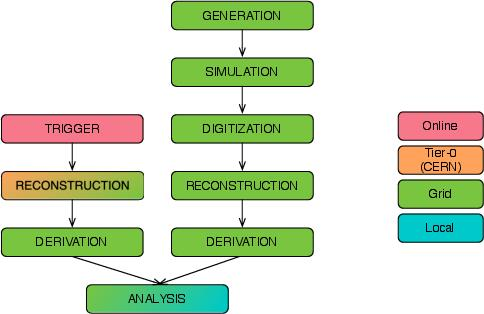
\includegraphics[width=0.9\linewidth]{dataFlow.png}
		\caption[Data flow for producing data and \acrshort{mc}.]{The data flow for producing data and \acrshort{mc}/background simulation. \acrshort{mc} start with Generation (right side) going through all the steps ending up with Analysis. Data start with a Trigger (left side) that picks out interesting events and information from a detector, e.g. the \acrshort{atlas} detector. \label{fig:DataFlow}}
	\end{figure}

	The data we use is proton-proton collisions at $\sqrt{13}=13$ TeV from the \acrshort{lhc} from the period 2015-2018. For the data we have a Trigger step that picks out interesting events. What is regarded as interesting is defined by the physicists depending on the analysis he/she wants to perform. In our case we trigger on three leptons with a given transverse momentum. This reduces the rate of writing data to disk. 
	
	The files we use for the \acrshort{mc} training in this thesis have only gone through the Generation step. We are then in full control over the truth origin, type (electron, muon, tau, quark etc.), $p_T$ etc. of the particles. The simulation is done using MadGraph\cite{MadGraph} with Pythia\cite{pythia} for showering/hadronization. The features we plot with \acrshort{mc} and data are after the Analysis step in Figure \ref{fig:DataFlow} with three leptons of good quality. For the \acrshort{ml} we want to use the \acrshort{ml} models on simulated backgrounds\footnote{Following the \acrshort{sm} processes.} and (neutrino) signal after the Analysis step. Now we no longer have the "truth" information about the particle types, the vertex it comes from etc. E.g. instead of a "true" electron we now have an electron object classified as an electron after it has passed a set of detector cuts. In some cases we get an electron is classified as a muon or a jet, causing some inefficiency with respect to the "true" distributions. Moreover, the energy and momentum resolution of the detector will smear the measurement of these quantities. In the case of the neutrino we know the full 4-vector at the truth level, while after the Reconstruction step we only see it as missing transverse energy with no information of its longitudinal component. We will just say we have three leptons and a neutrino/\acrshort{met} in each event to distinguish easier in this thesis, even though the neutrino is a lepton.


	\section{Feature Validation}
	\label{sect:Method-Features}
	We will now take a look at the features in the \acrshort{mc} and signal Ntuples we will be using in this thesis. The Ntuples all contain the same features with separate variables for the three leptons, e.g. Charge, Flavor, Pt, Eta and Phi. We also use a feature to define twp cuts on the events that only contain 3 leptons, \textit{nLep\_base}==3 and \textit{nLep\_signal}==3. Since we do not know the truth information of the leptons in these Ntuples, the leptons in each event are arranged such that lepton 1 of an event has the highest momentum, lepton 2 has the second highest and so on. This does not mean that lepton 1 actually comes from vertex 1. For the neutrino we only have the met\_Et and met\_Phi features.
	
	In Figure \ref{fig:Flavor_Charge} we see the data, \acrshort{mc} and signal plots for the Flavor and Charge of the three leptons. The Flavor figures show either 1 or 2 as lepton flavor values corresponding to electron and muon, respectively. The Charge figures show that the leptons can either have -1 or 1 as values.
	
	In Figure \ref{fig:Eta_Phi} we see the data, \acrshort{mc} and signal plots of Eta and Phi for the three leptons. The eta values are between -2.5 and 2.5, while the phi values are between $-\pi$ and $\pi$.
	
	In Figure \ref{fig:Pt_orig} we see the Pt of the three leptons. As expected, since the arrangement of the leptons are after $p_T$ lepton 1 has a long tail towards high $p_T$ reaching beyond 800 GeV. Lepton 2 has only a few events around 800 GeV, while $p_T$ of lepton 3 reaches only to about 500 GeV. All distributions have most events at low $p_T$ and decreasing as $p_T$ increases. The smaller signal with mass $N_1=150$ GeV reaches its peak much earlier than the 450 GeV signal in all $p_T$ figures. This makes sense since the signal with higher mass neutrino will have more events with high energy leptons.
	
	Met\_Et and met\_Phi are seen in Figure \ref{fig:MET_orig}. The Phi feature is very similar to the Phi feature for the three lepton, where the number of events is more or less equal for all values of $\phi$. The transverse energy, or $E_T^{\text{miss}}$, reaches to 600 GeV. Like for the $p_T$ of the leptons, the smaller signal reaches its peak much earlier and has fewer events with higher $p_T$.
	
	A thing to notice from these figures is the poor compliance between data and \acrshort{mc} for $p_T$ and \acrshort{met} after around 200 GeV. The optimal case would have all the dots in the lower frames on the 1-marked line. The reason for this difference is not known to us. It might be from bad modeling, but this error goes beyond this thesis.
	
	\begin{figure}[h!]
		\vspace*{-4.5cm}
		\hspace*{-1.cm}
		\subfloat[Flavor lepton 1\label{subfig:Flavor1}]{\centering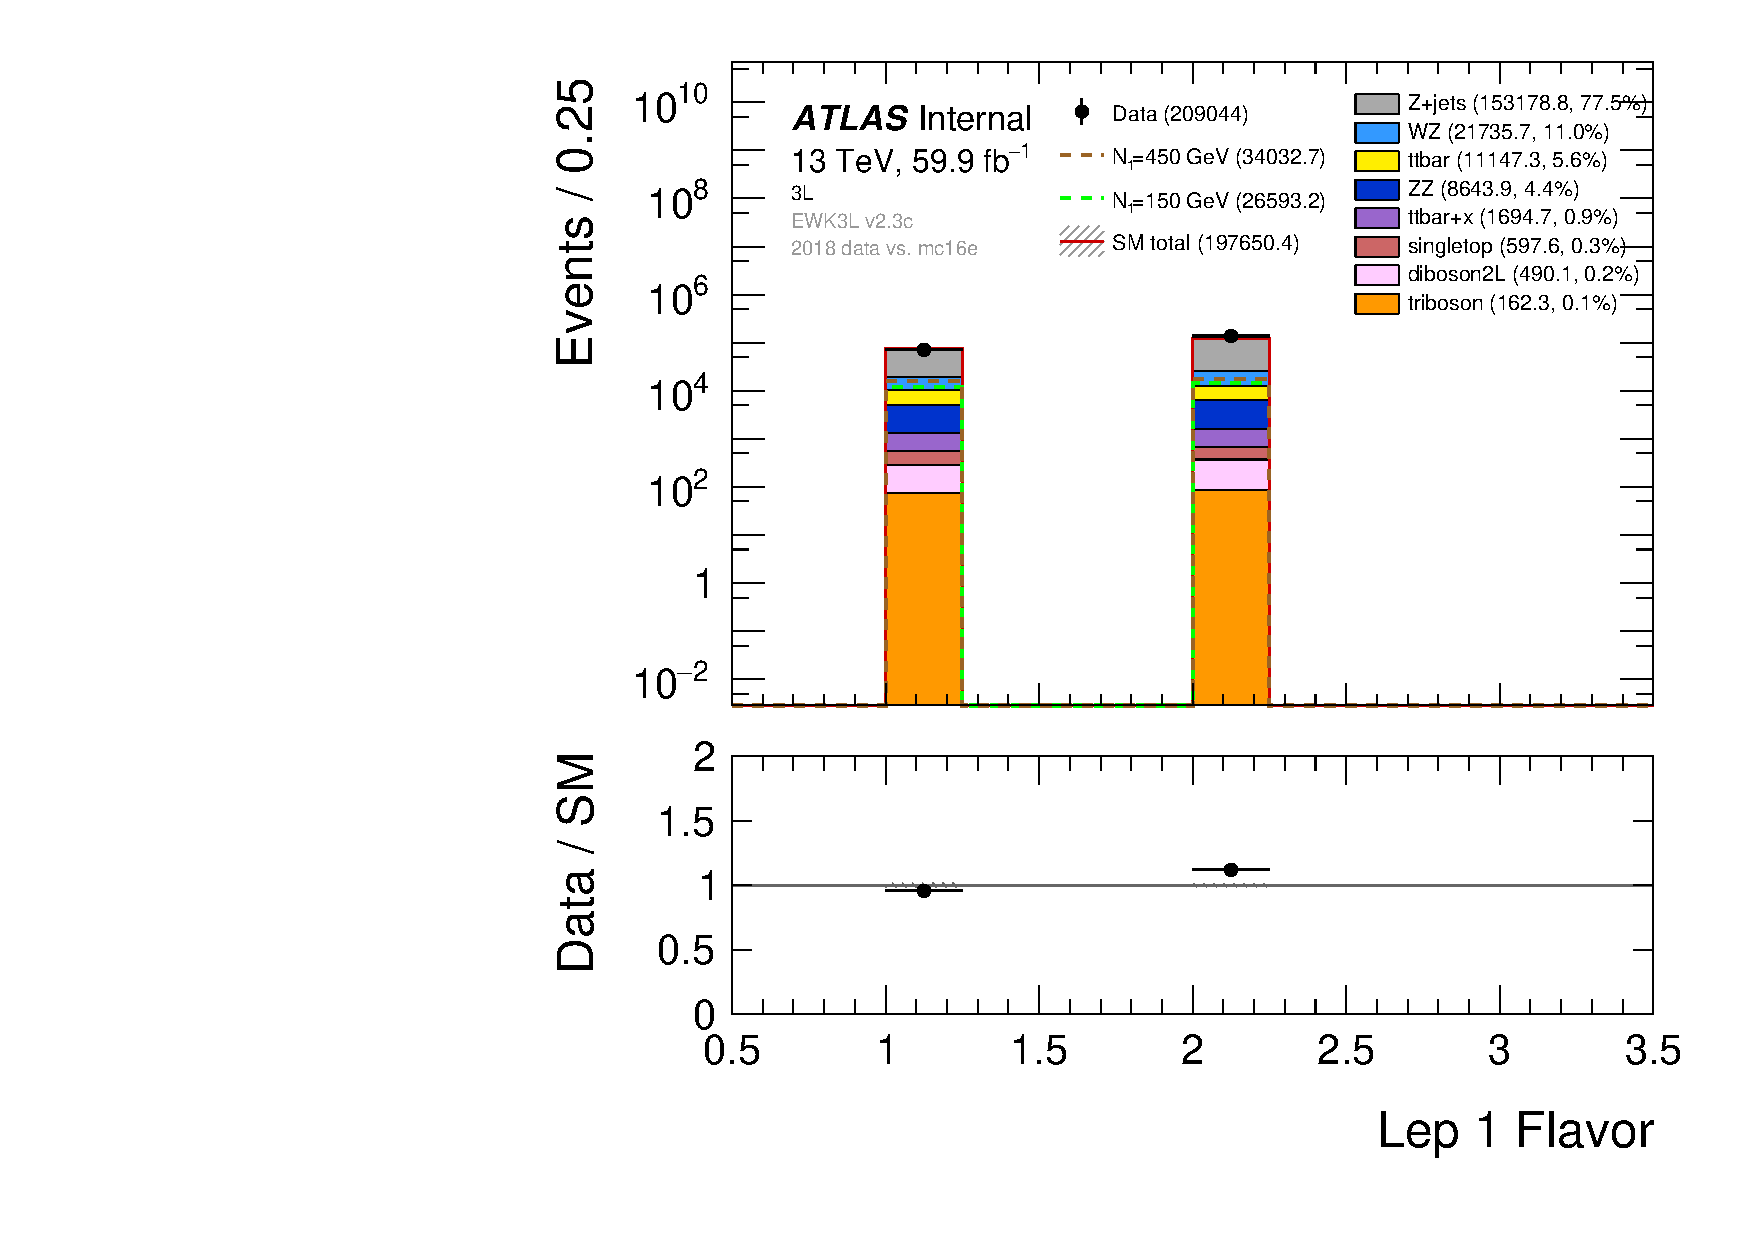
\includegraphics[width=0.55\linewidth]{ROOT_plots/hist1d_lep1Flavor_3L.pdf}}
		\subfloat[Charge lepton 1\label{subfig:Charge1}]{\centering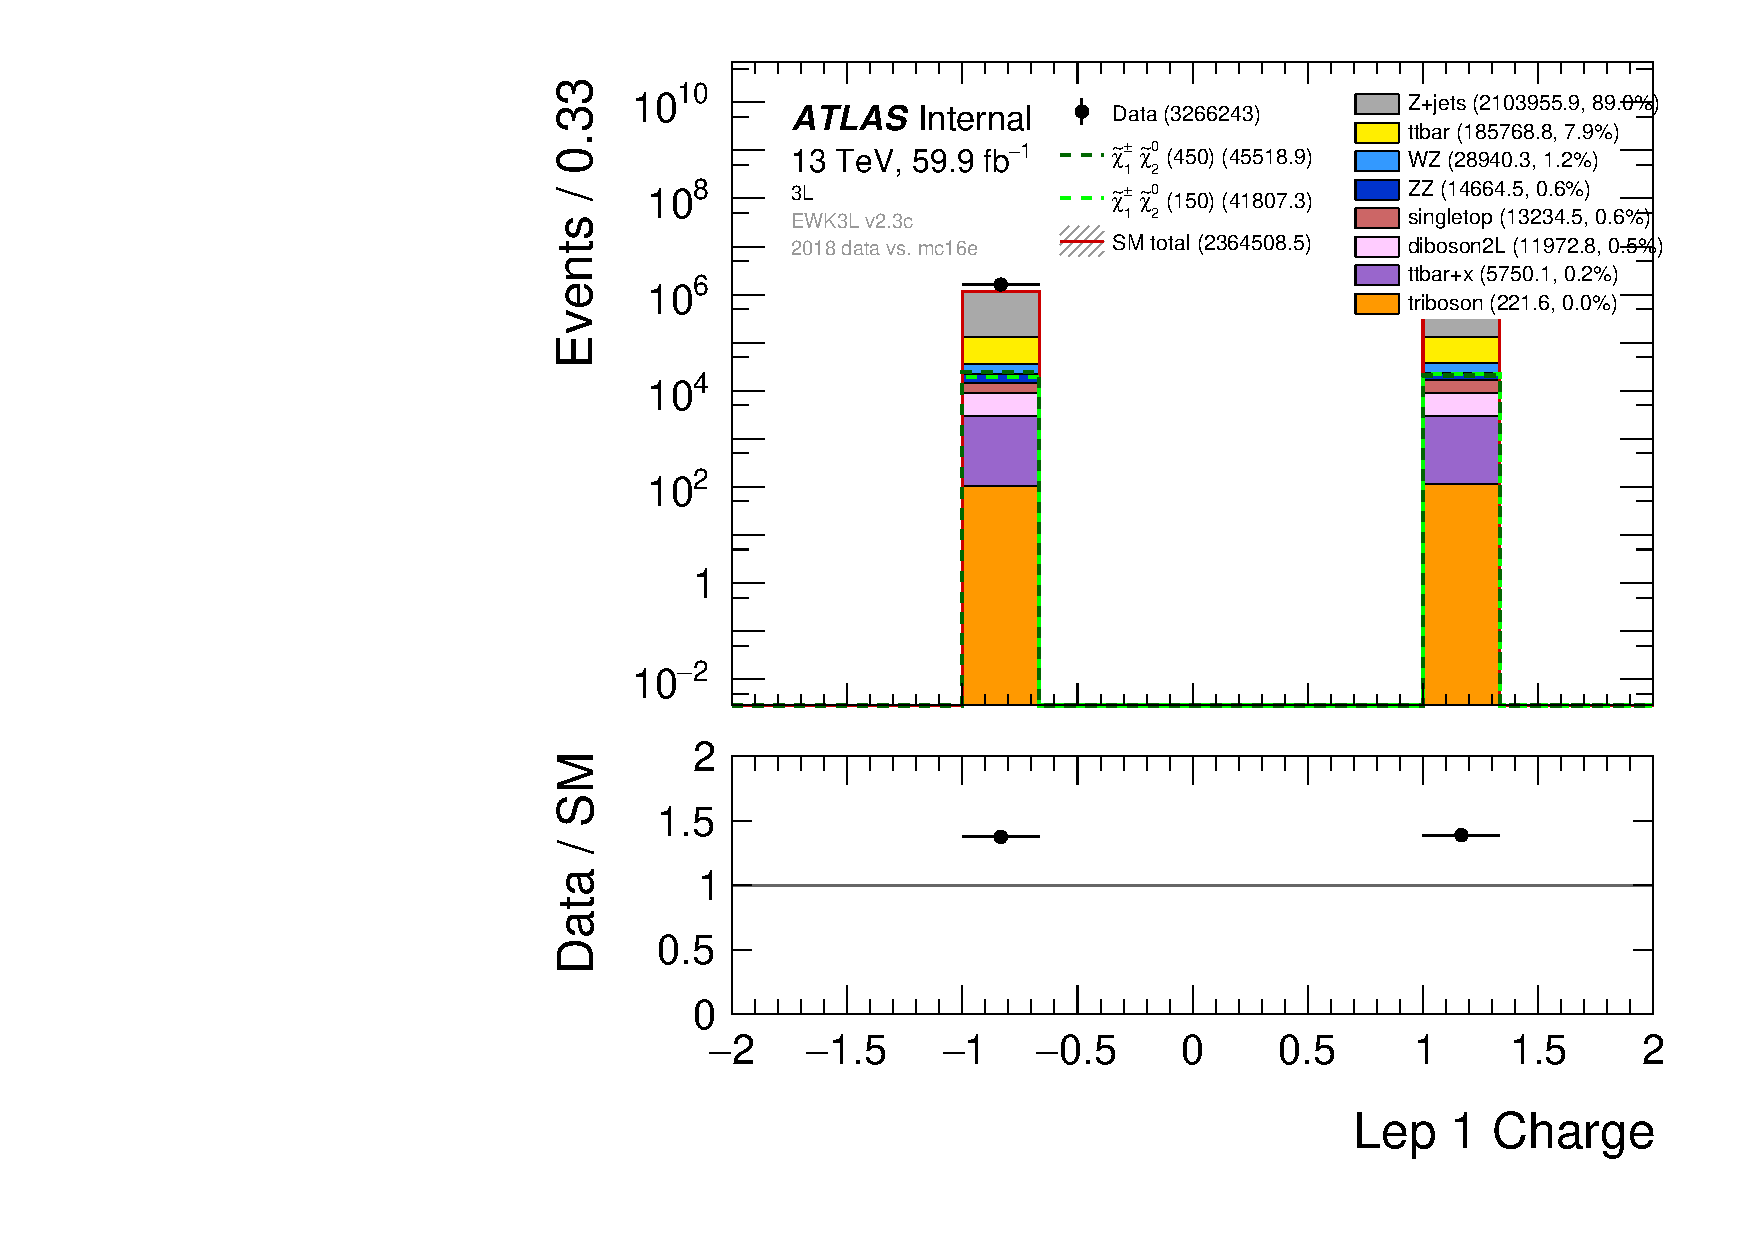
\includegraphics[width=0.55\linewidth]{ROOT_plots/hist1d_lep1Charge_3L.pdf}}\\
		\hspace*{-1.cm}
		\subfloat[Flavor lepton 2\label{subfig:Flavor2}]{\centering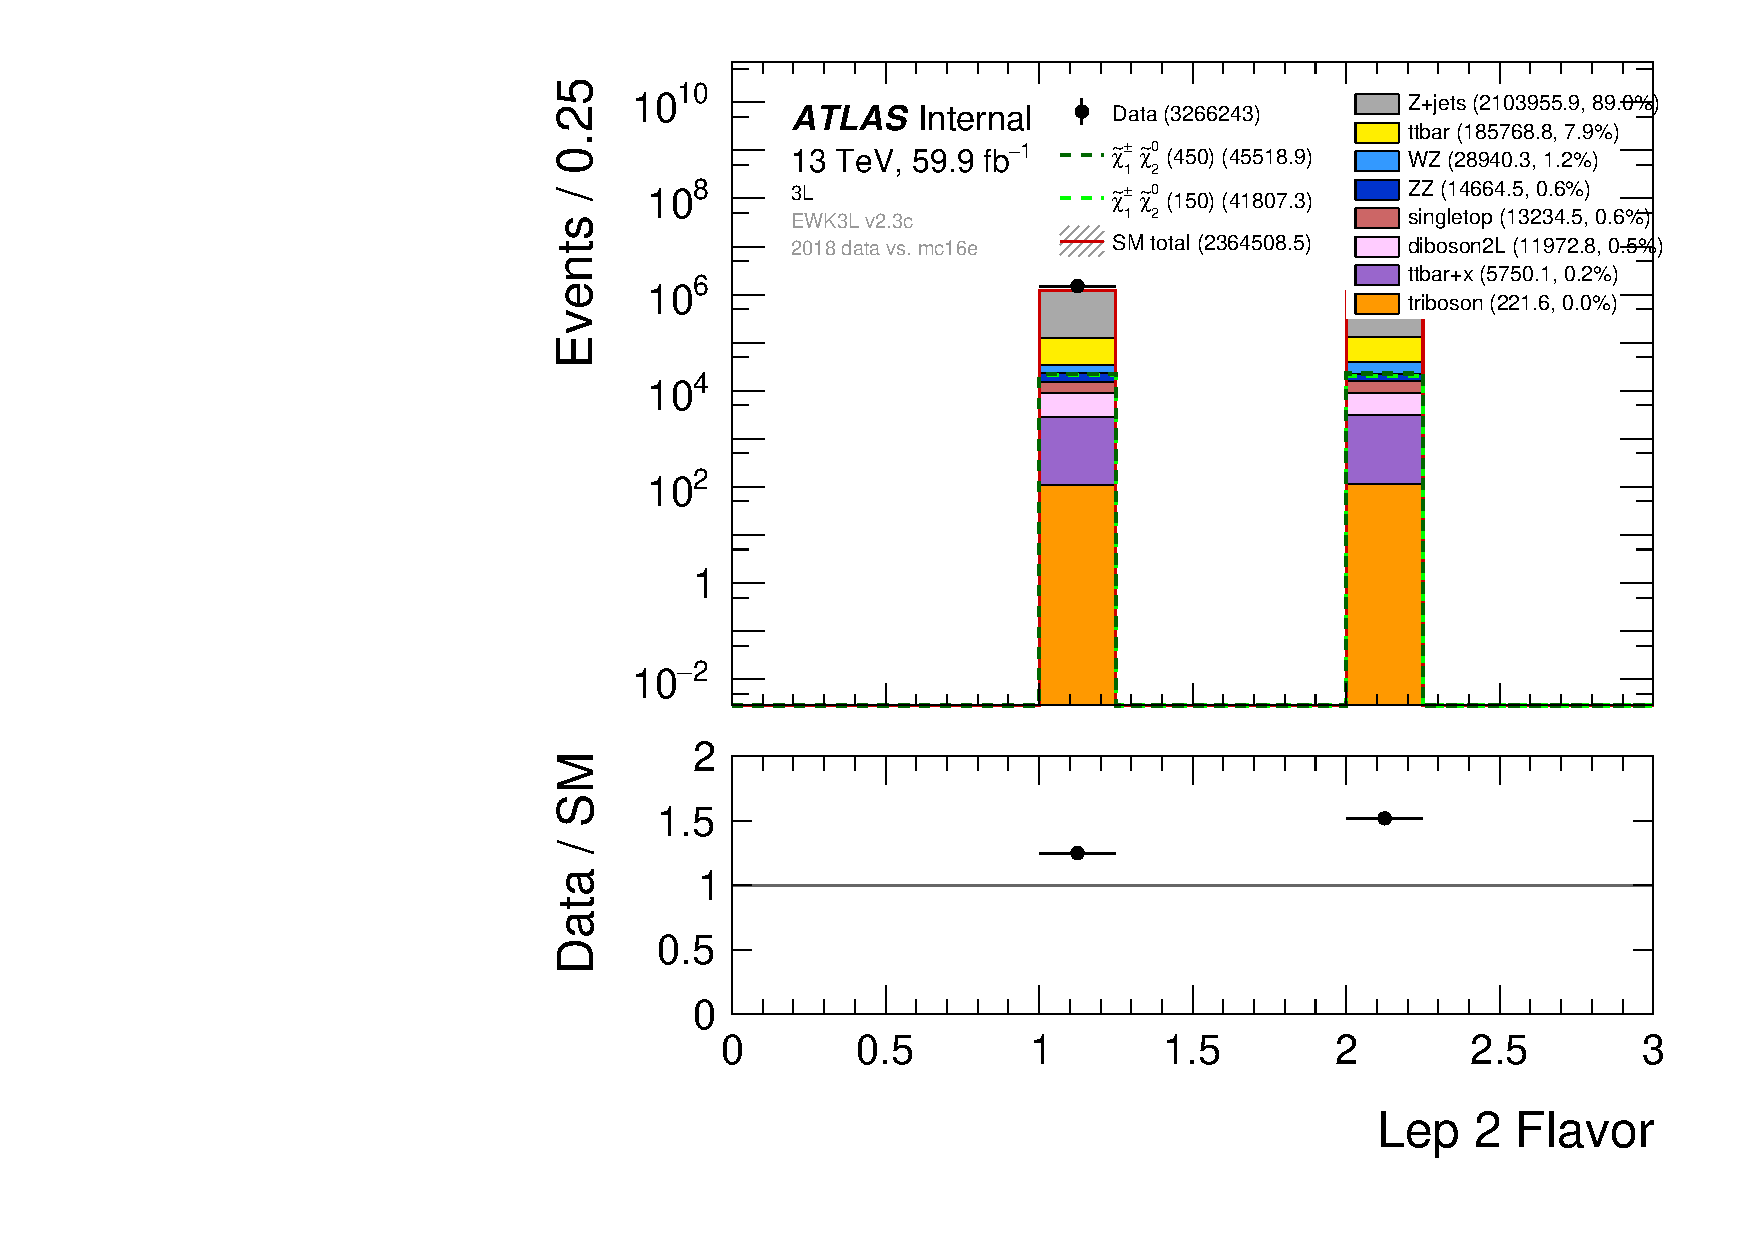
\includegraphics[width=0.55\linewidth]{ROOT_plots/hist1d_lep2Flavor_3L.pdf}}
		\subfloat[Charge lepton 2\label{subfig:Charge2}]{\centering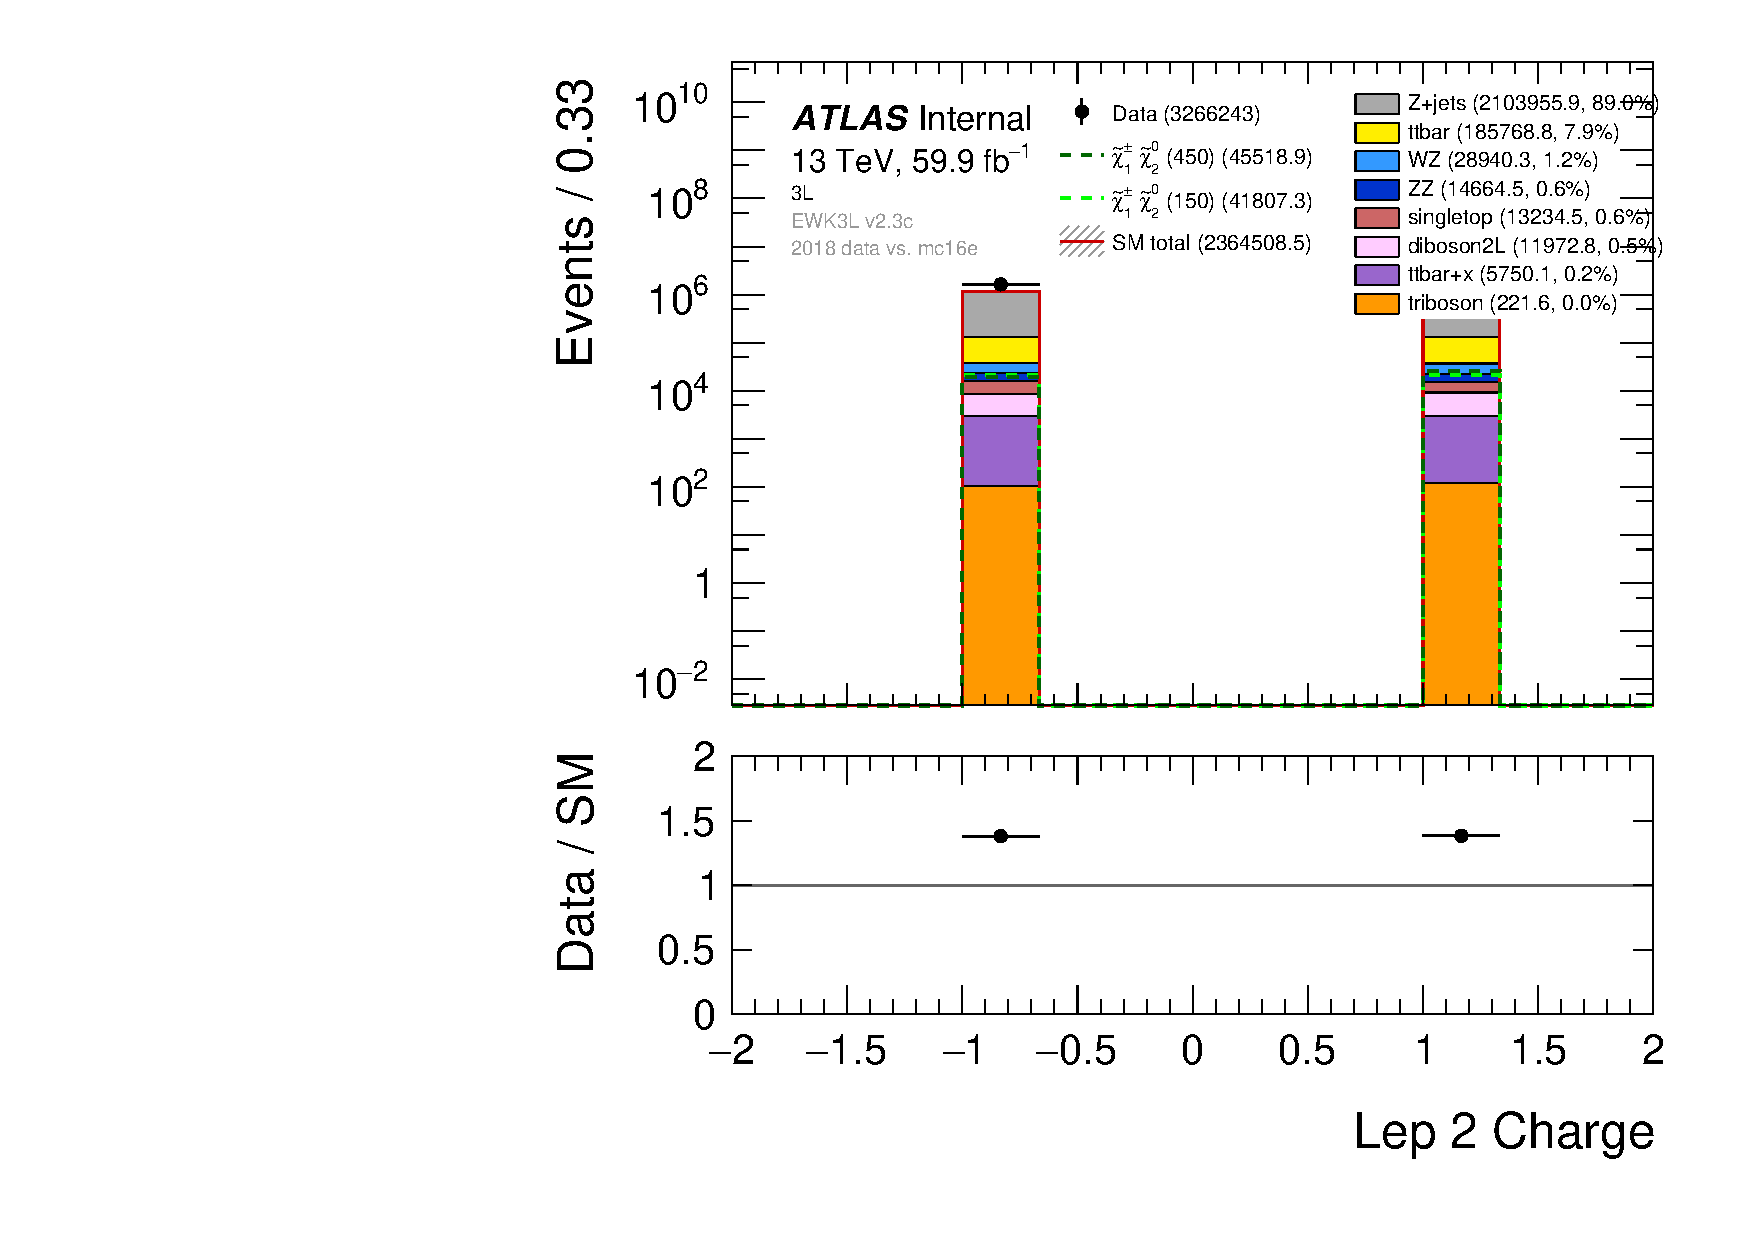
\includegraphics[width=0.55\linewidth]{ROOT_plots/hist1d_lep2Charge_3L.pdf}}\\
		\hspace*{-1.cm}
		\subfloat[Flavor lepton 3\label{subfig:Flavor3}]{\centering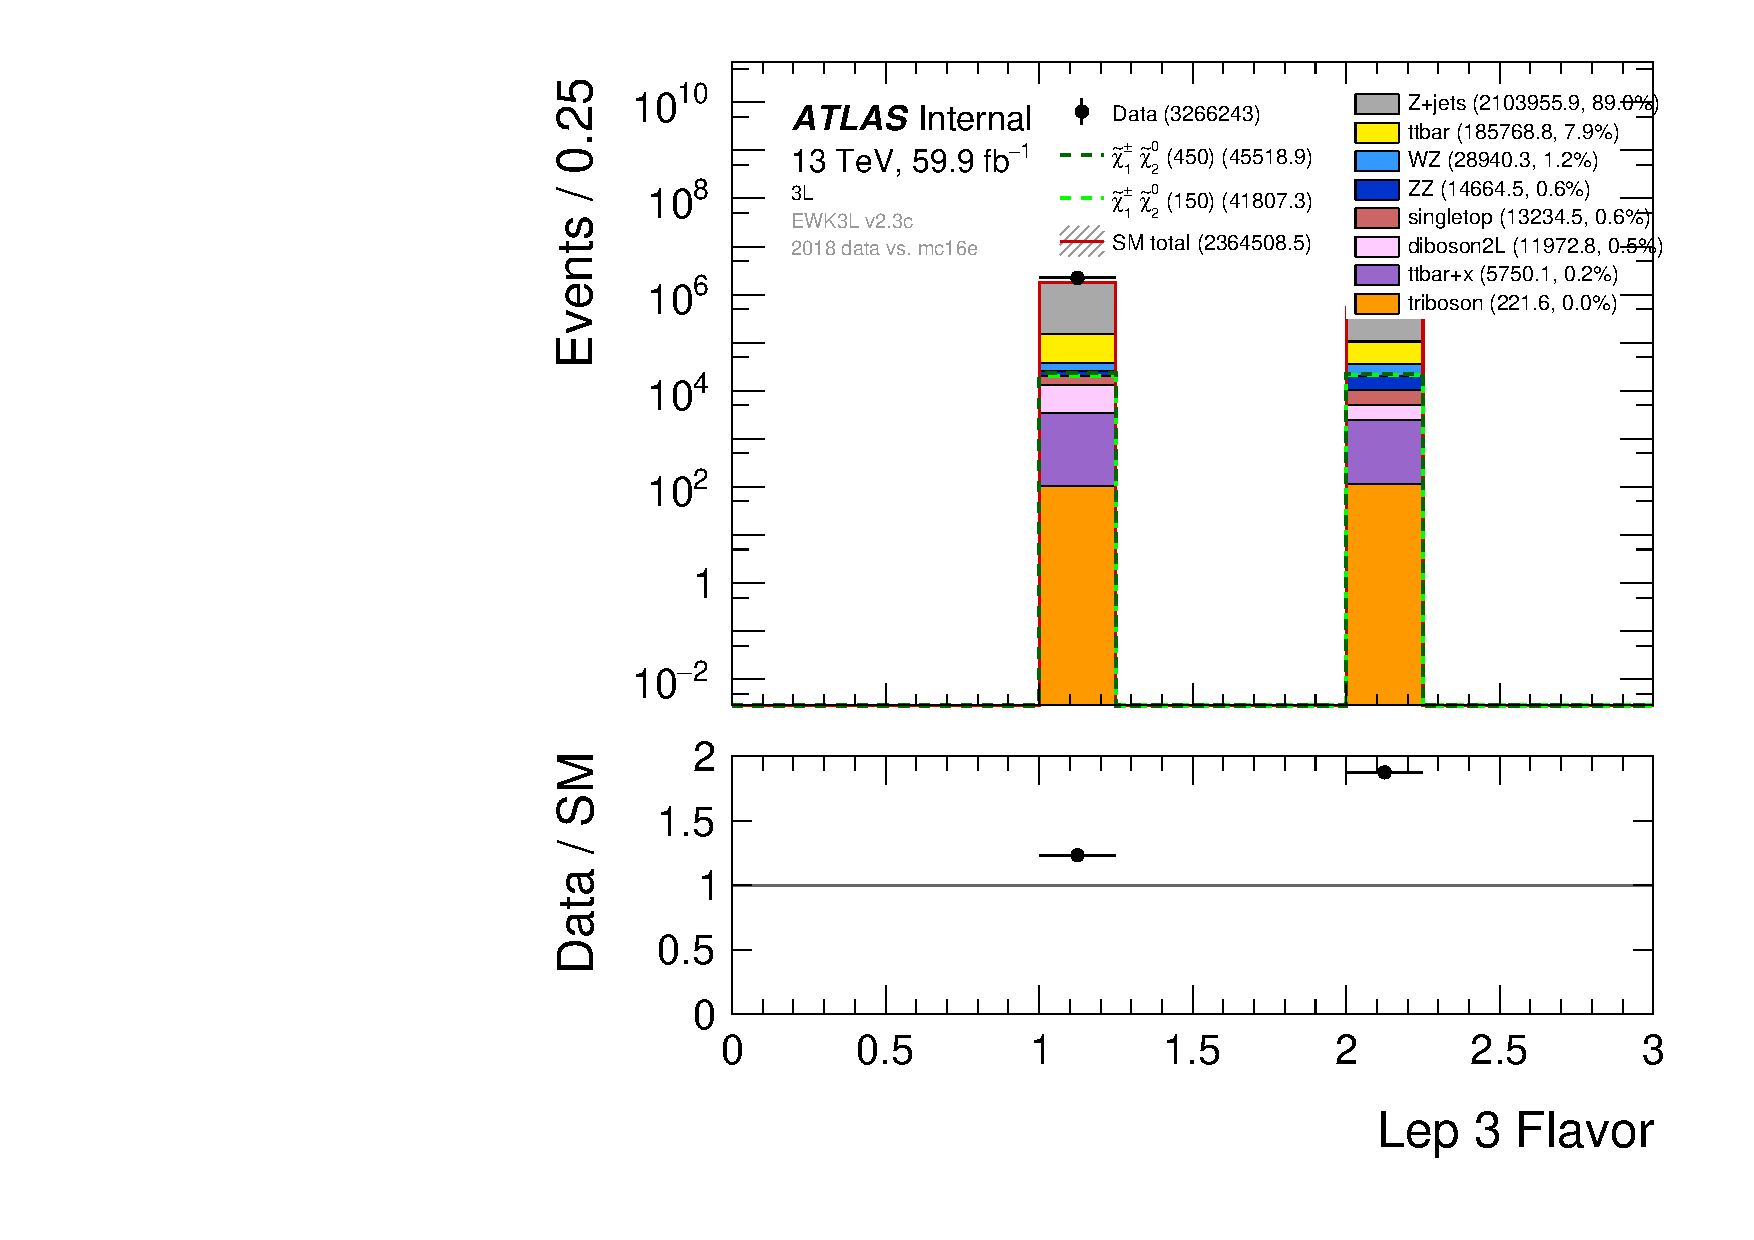
\includegraphics[width=0.55\linewidth]{ROOT_plots/hist1d_lep3Flavor_3L.pdf}}
		\subfloat[Charge lepton 3\label{subfig:Charge3}]{\centering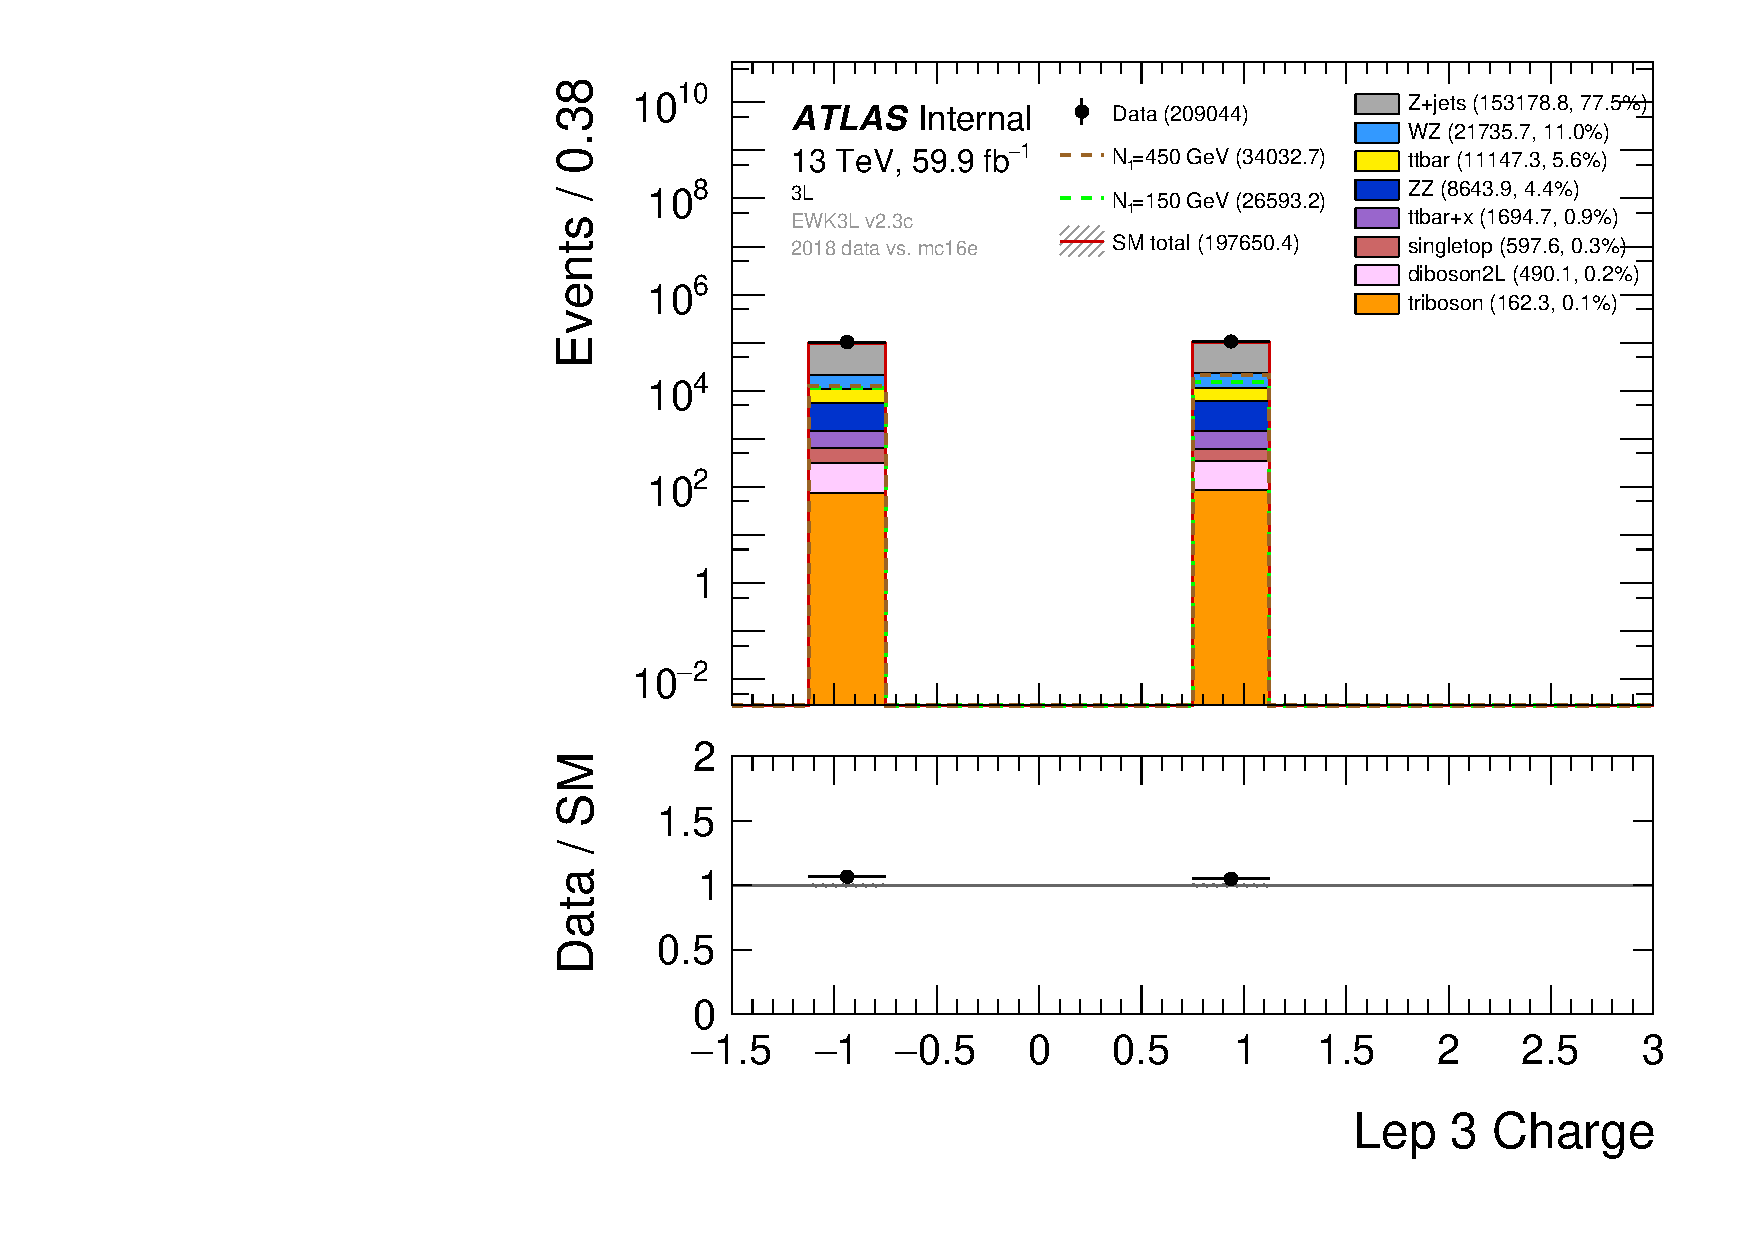
\includegraphics[width=0.55\linewidth]{ROOT_plots/hist1d_lep3Charge_3L.pdf}}
		\caption[Flavor and Charge plots for the three leptons.]{Plot of the Flavor and Charge features for the three leptons with data, \acrshort{mc} and two neutrino signals. The flavor of the leptons can either be 1 (an electron) or 2 (a muon), while the charge of the leptons can be either -1 or 1. \label{fig:Flavor_Charge}}
	\end{figure}
	
	\begin{figure}[h!]
		\vspace*{-4.5cm}
		\hspace*{-1.cm}
		\subfloat[Eta lepton 1\label{subfig:Eta1}]{\centering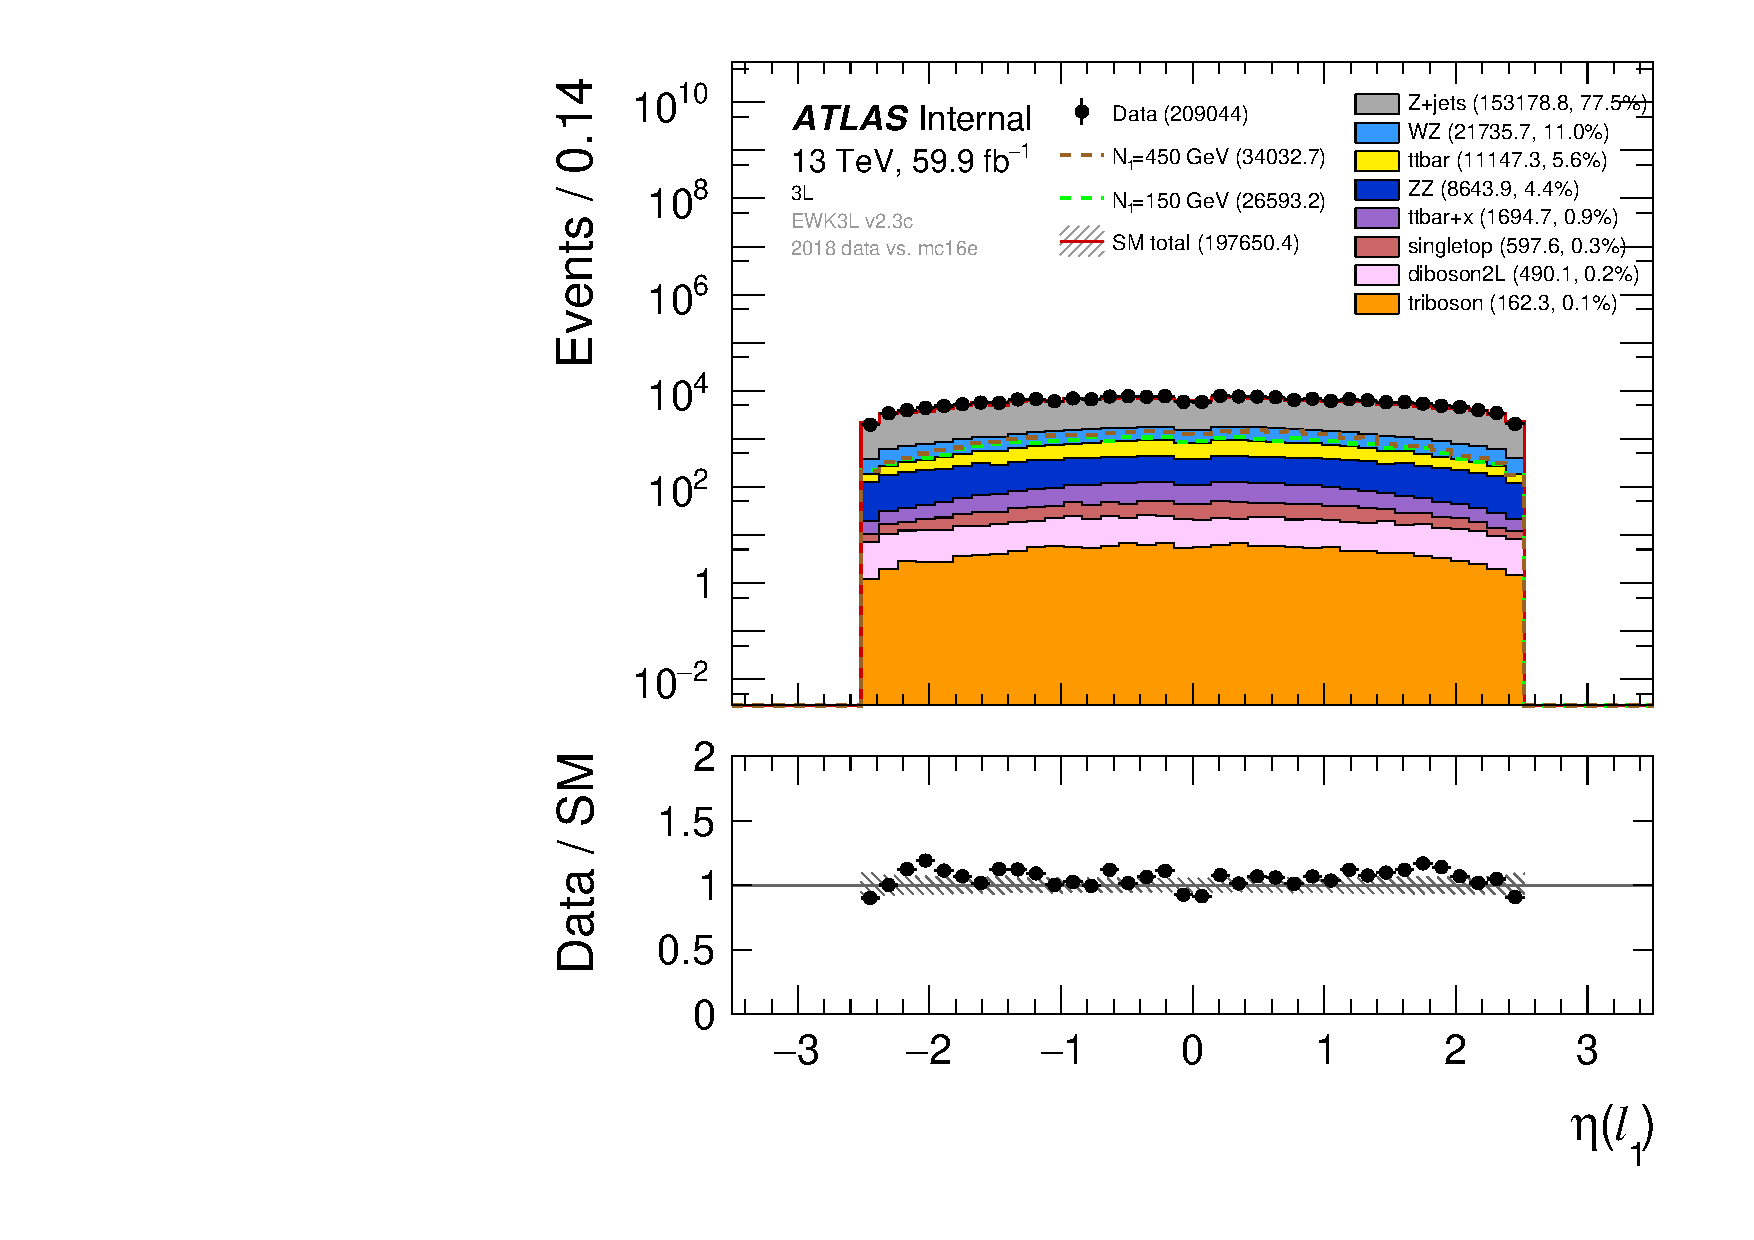
\includegraphics[width=0.55\linewidth]{ROOT_plots/hist1d_lep1Eta_3L.pdf}}
		\subfloat[Phi lepton 1\label{subfig:Phi1}]{\centering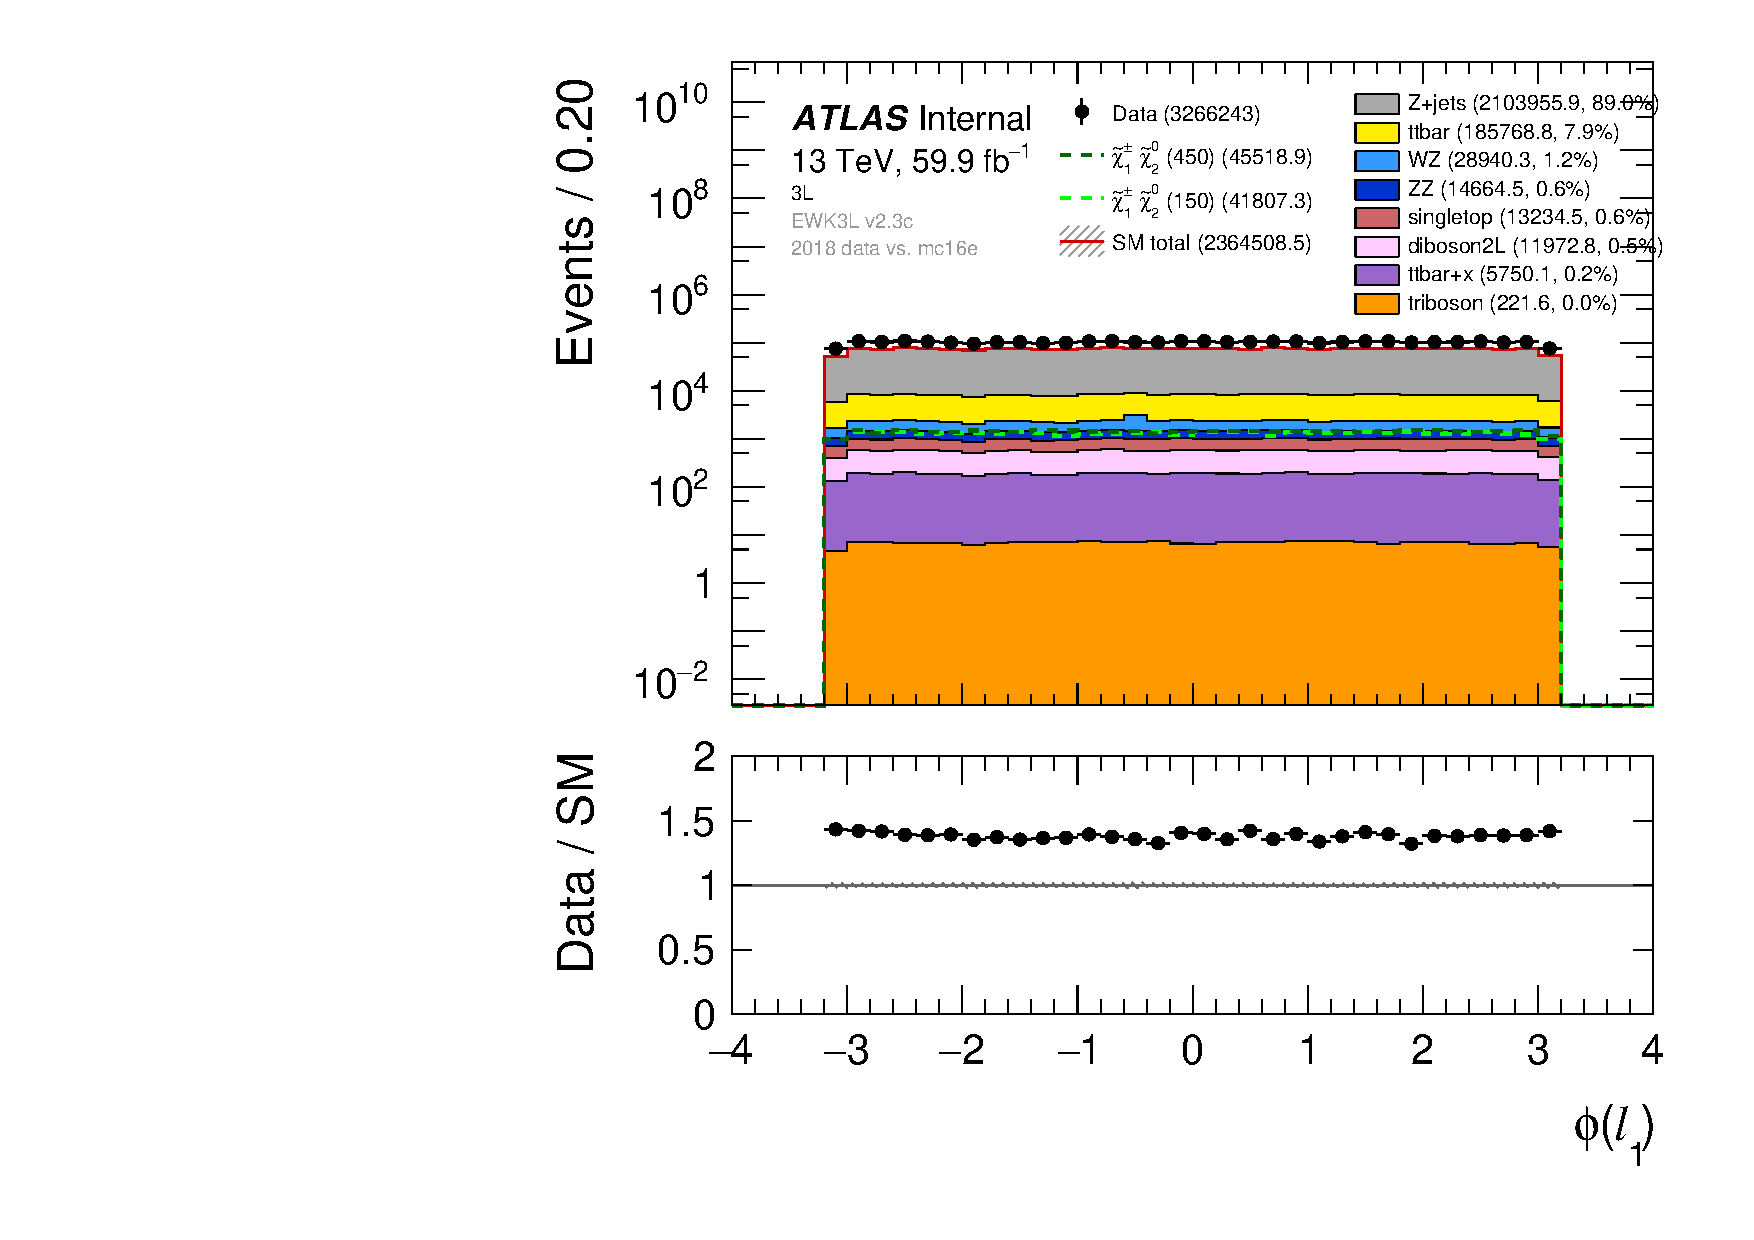
\includegraphics[width=0.55\linewidth]{ROOT_plots/hist1d_lep1Phi_3L.pdf}}\\
		\hspace*{-1.cm}
		\subfloat[Eta lepton 2\label{subfig:Eta2}]{\centering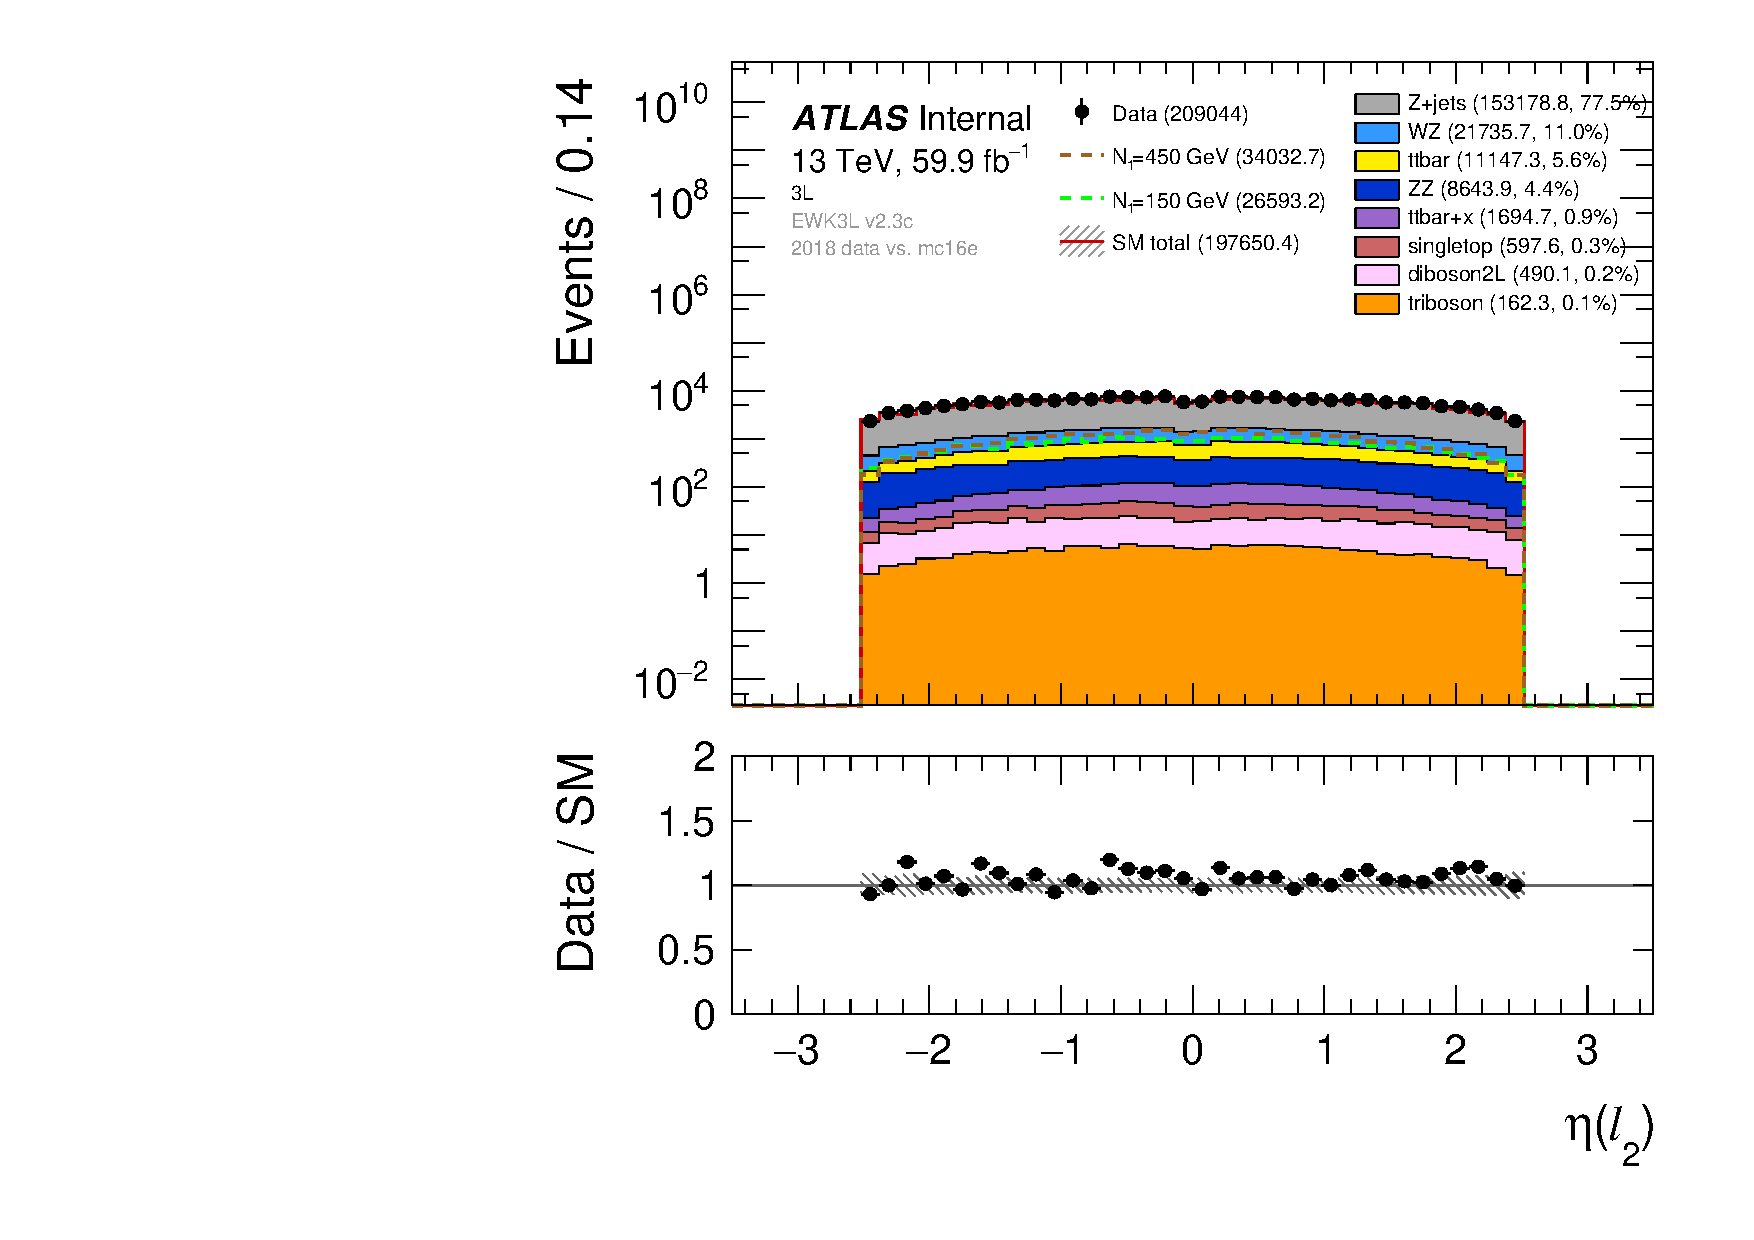
\includegraphics[width=0.55\linewidth]{ROOT_plots/hist1d_lep2Eta_3L.pdf}}
		\subfloat[Phi lepton 2\label{subfig:Phi2}]{\centering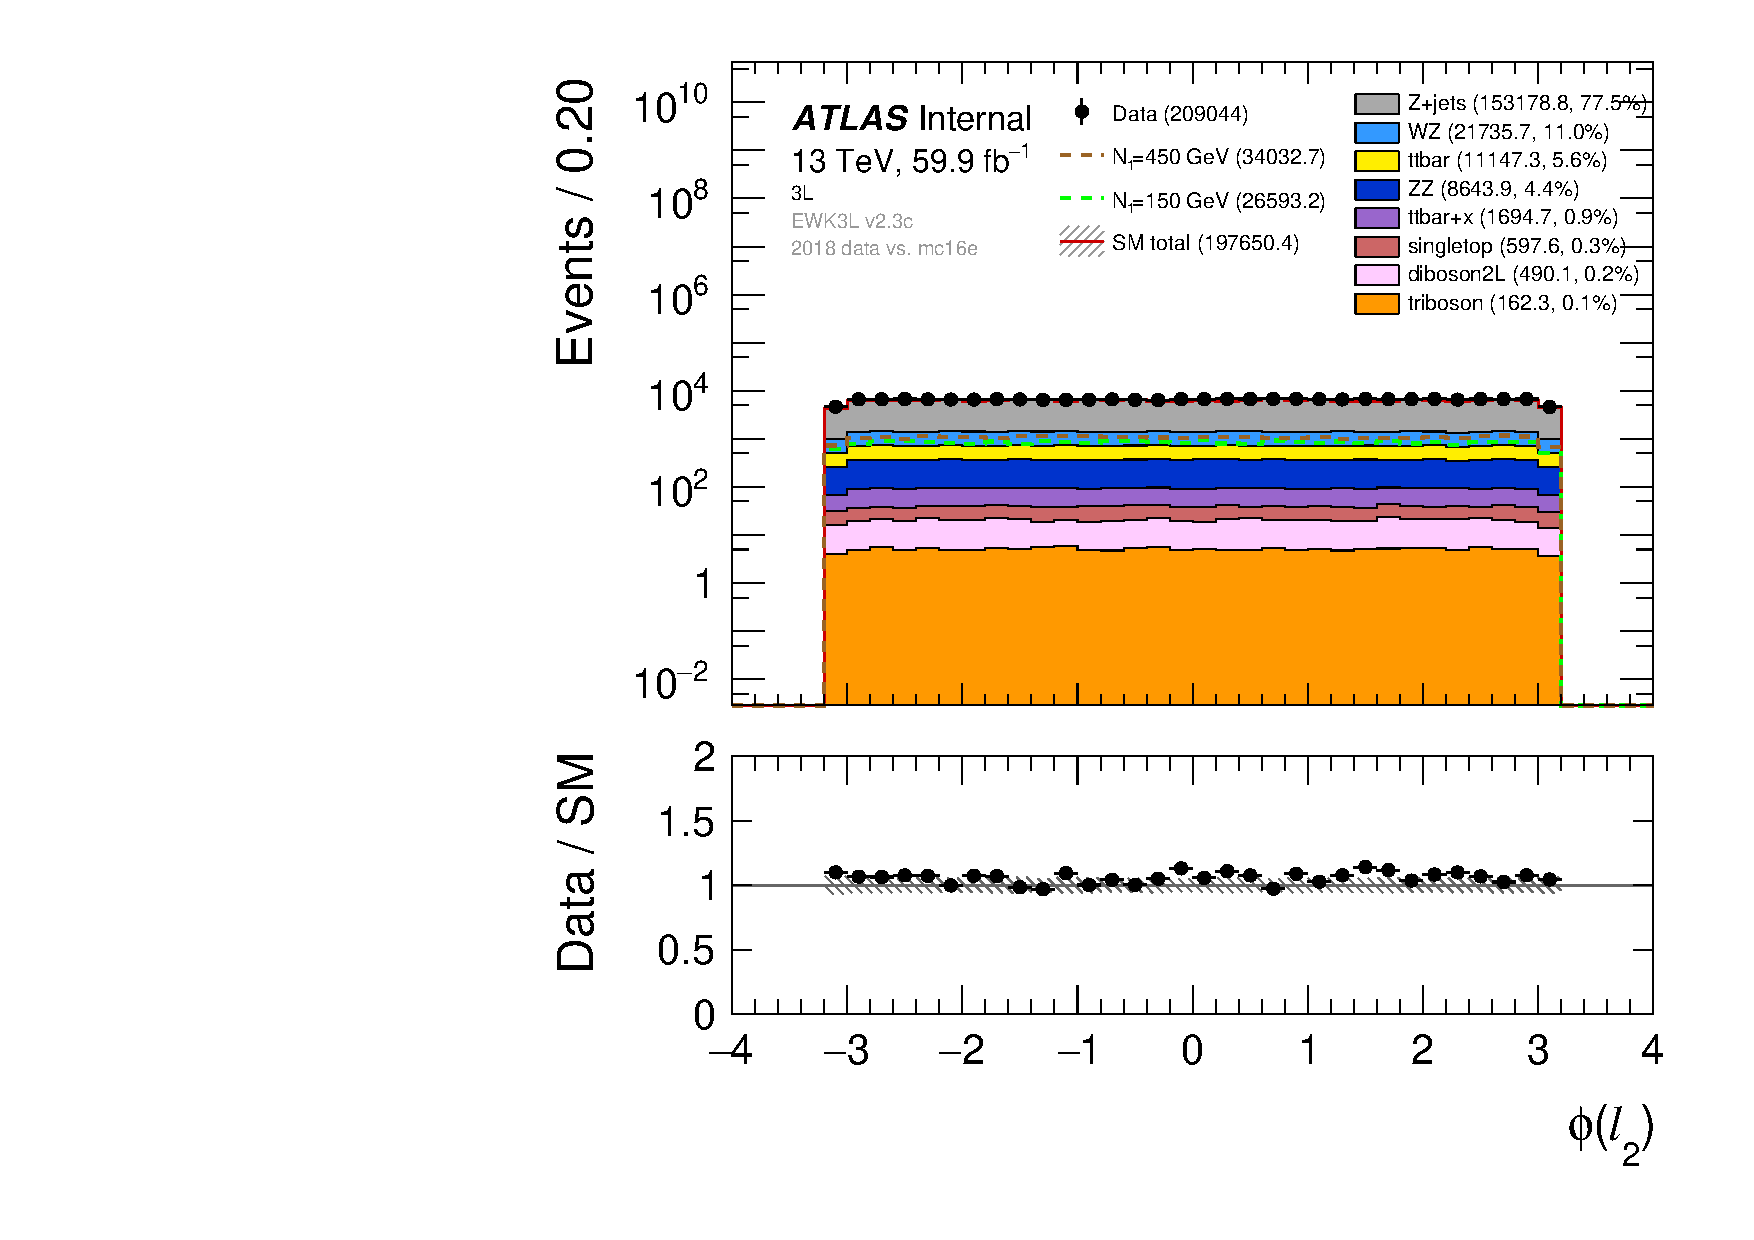
\includegraphics[width=0.55\linewidth]{ROOT_plots/hist1d_lep2Phi_3L.pdf}}\\
		\hspace*{-1.cm}
		\subfloat[Eta lepton 3\label{subfig:Eta3}]{\centering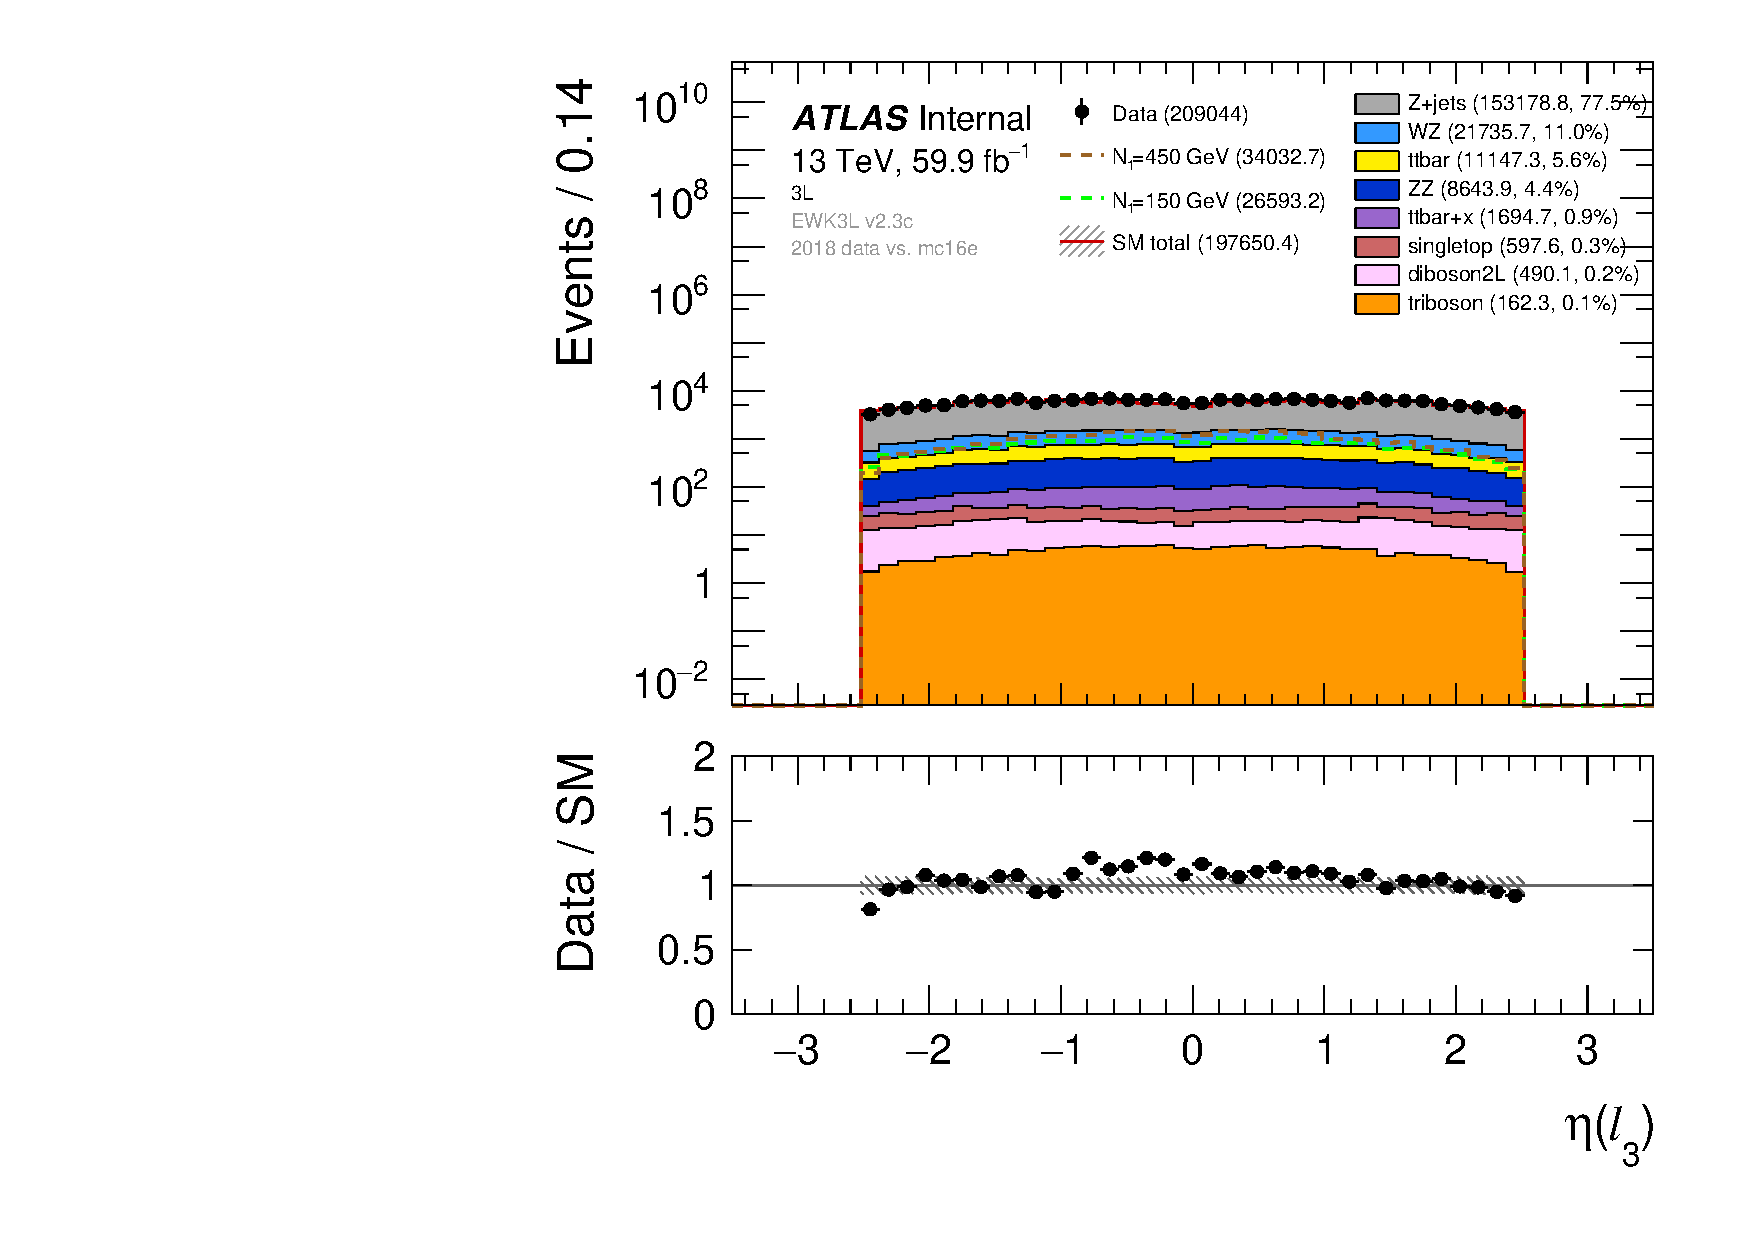
\includegraphics[width=0.55\linewidth]{ROOT_plots/hist1d_lep3Eta_3L.pdf}}
		\subfloat[Phi lepton 3\label{subfig:Phi3}]{\centering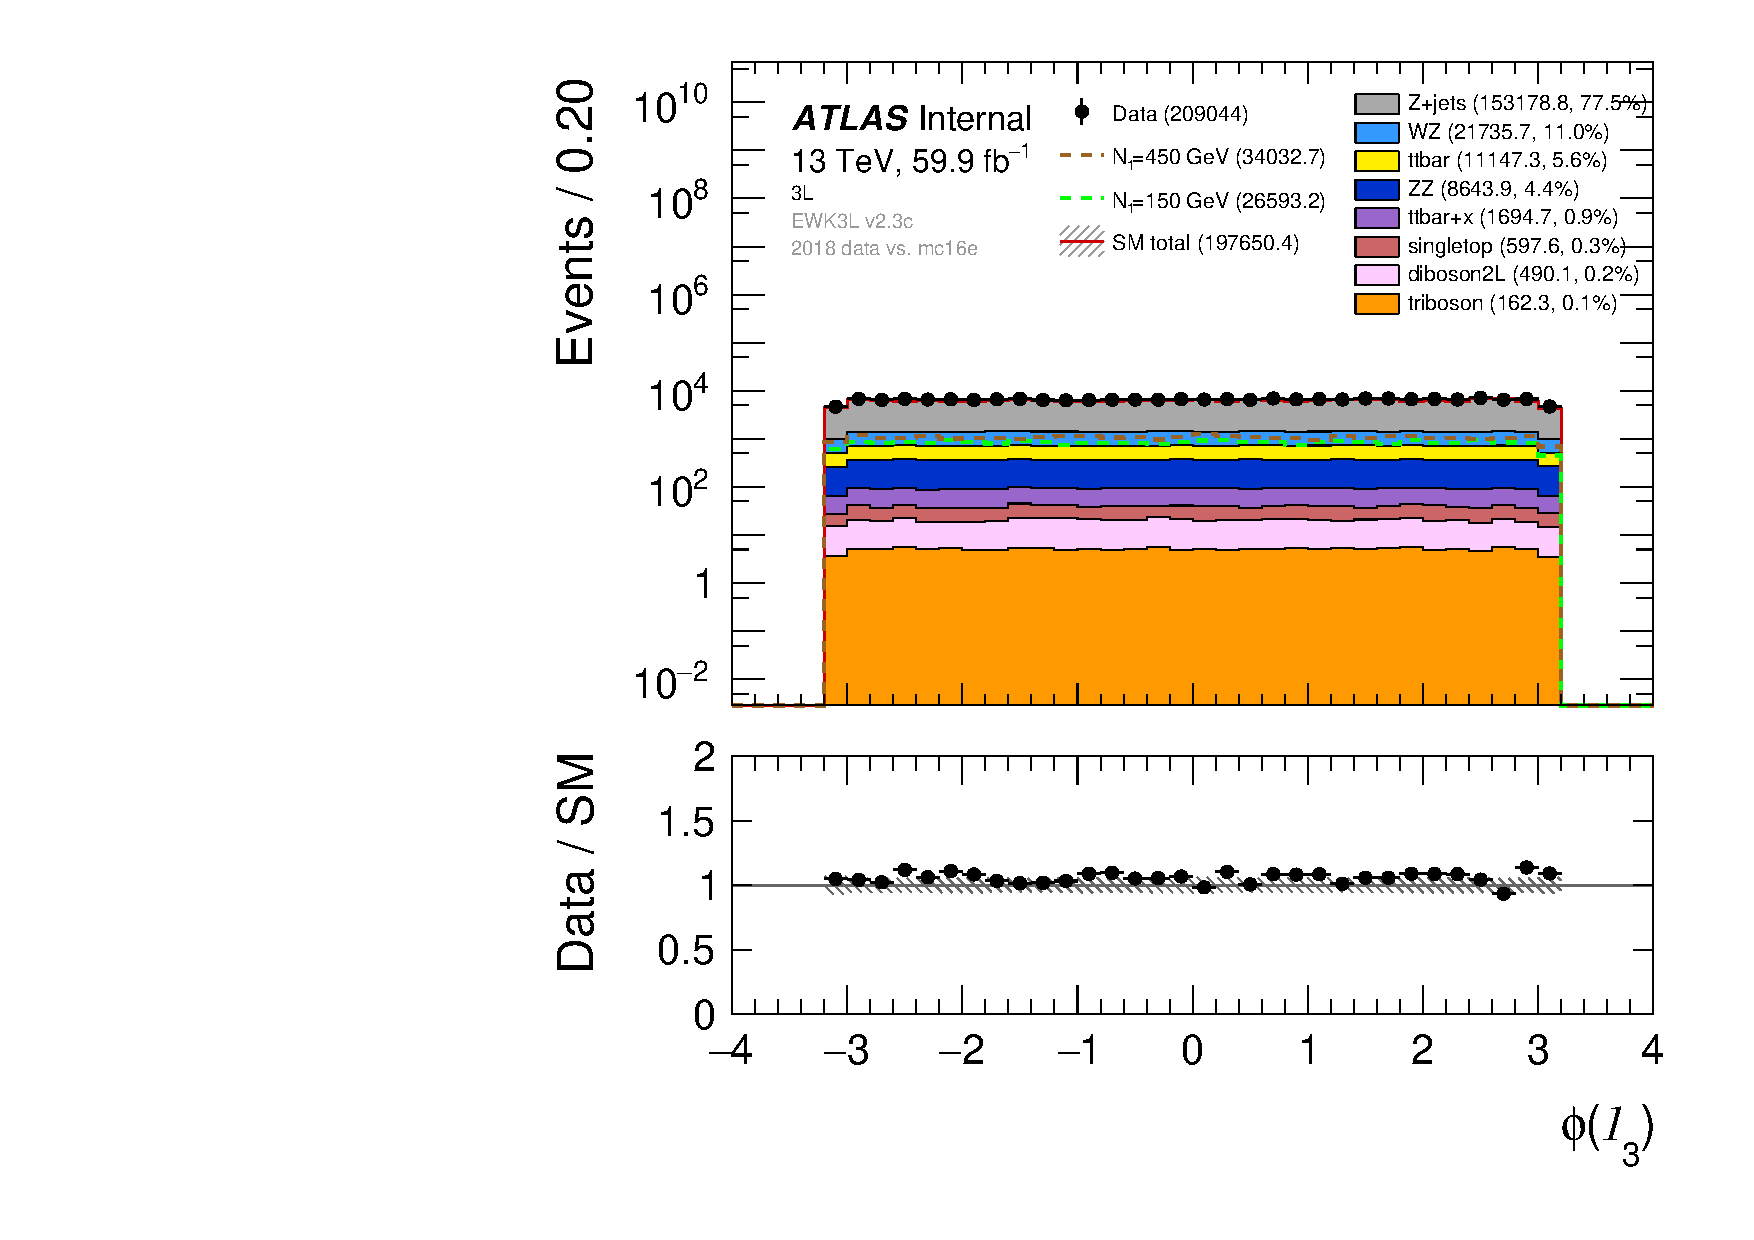
\includegraphics[width=0.55\linewidth]{ROOT_plots/hist1d_lep3Phi_3L.pdf}}
		\caption[Eta and Phi plots for the three leptons.]{Plot of the Eta and Phi for the three leptons with data, \acrshort{mc} and two neutrino signals. All distributions show very little dependence on phi/eta. \label{fig:Eta_Phi}}
	\end{figure}

	\begin{figure}[htb!]
		\hspace*{-1.cm}
		\subfloat[Pt lepton 1\label{subfig:Pt1}]{\centering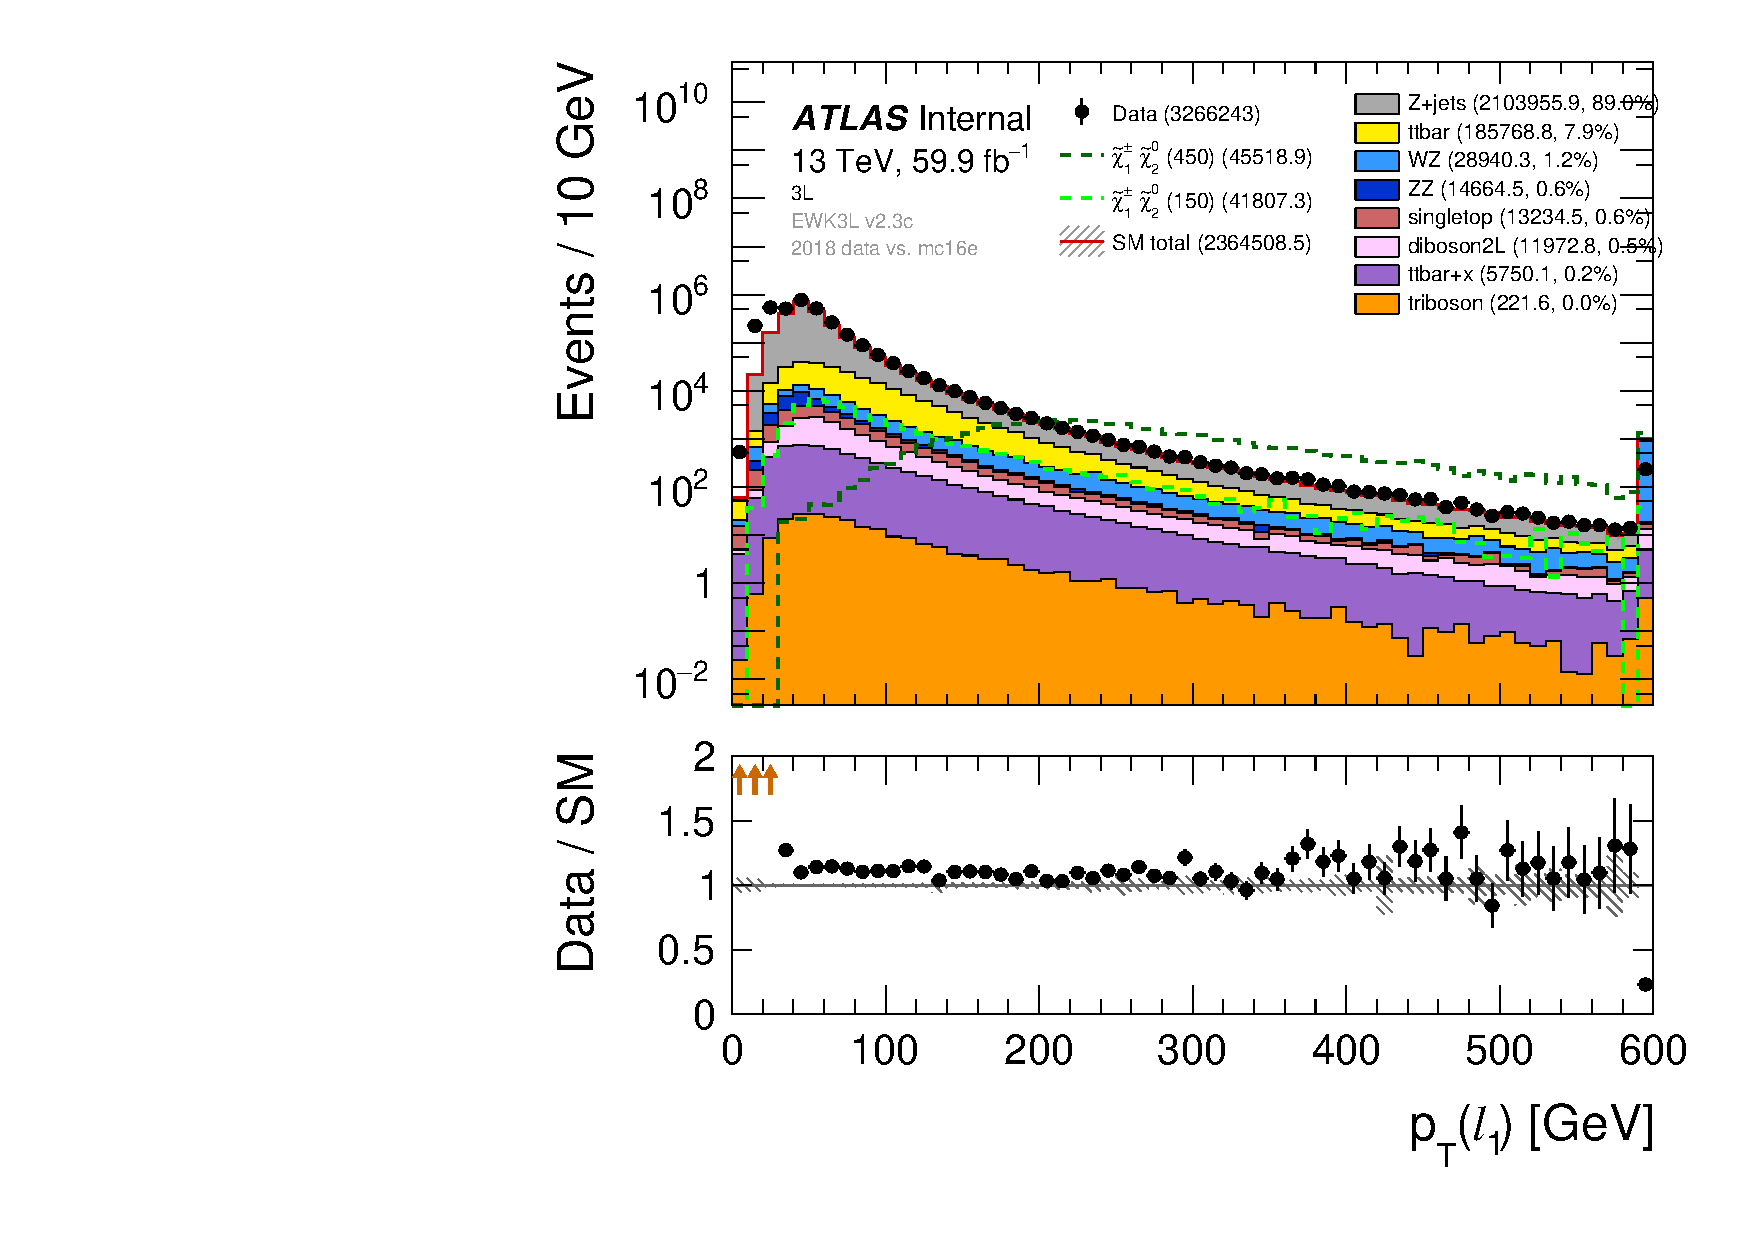
\includegraphics[width=0.55\linewidth]{ROOT_plots/hist1d_lep1Pt_3L.pdf}}
		\subfloat[Pt lepton 2\label{subfig:P2}]{\centering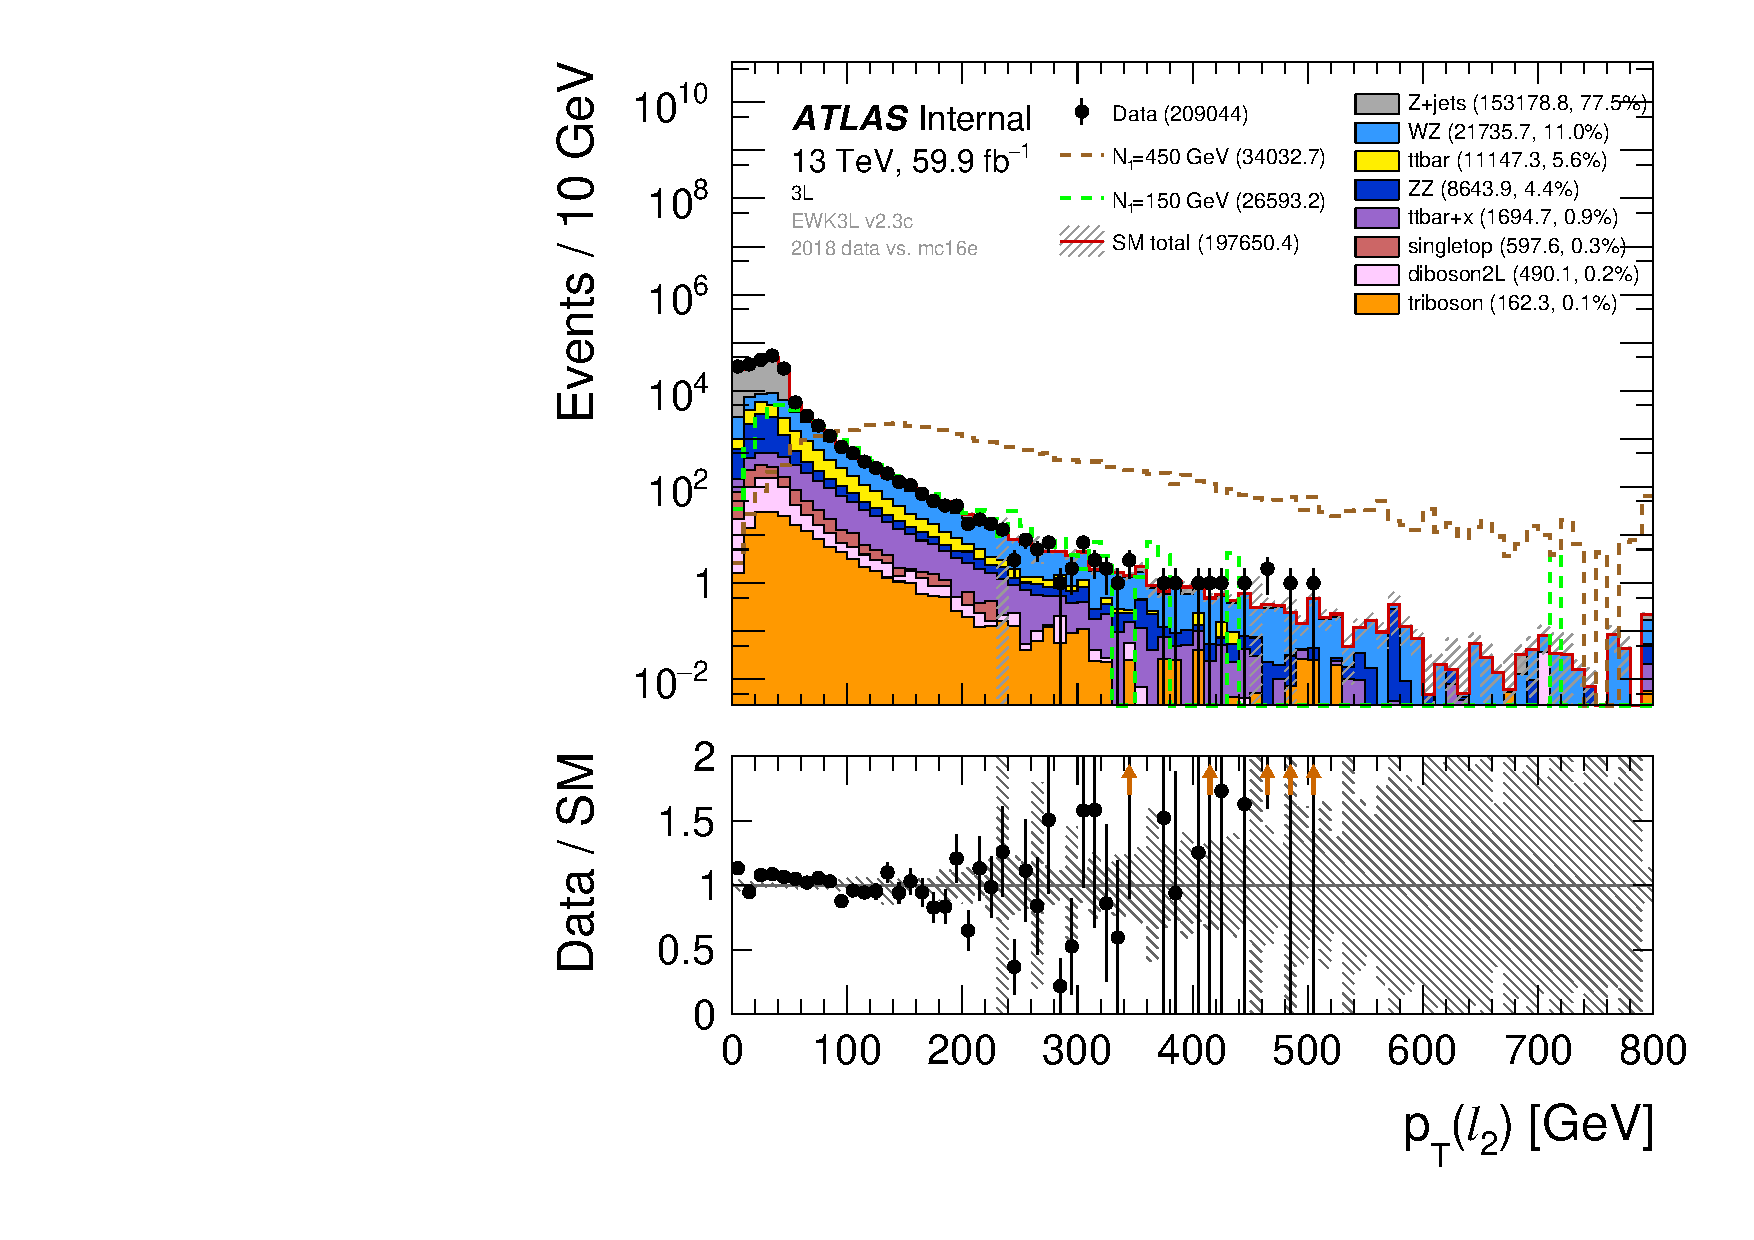
\includegraphics[width=0.55\linewidth]{ROOT_plots/hist1d_lep2Pt_3L.pdf}}\\
		\hspace*{3.cm}
		\subfloat[Pt lepton 3\label{subfig:Pt3}]{\centering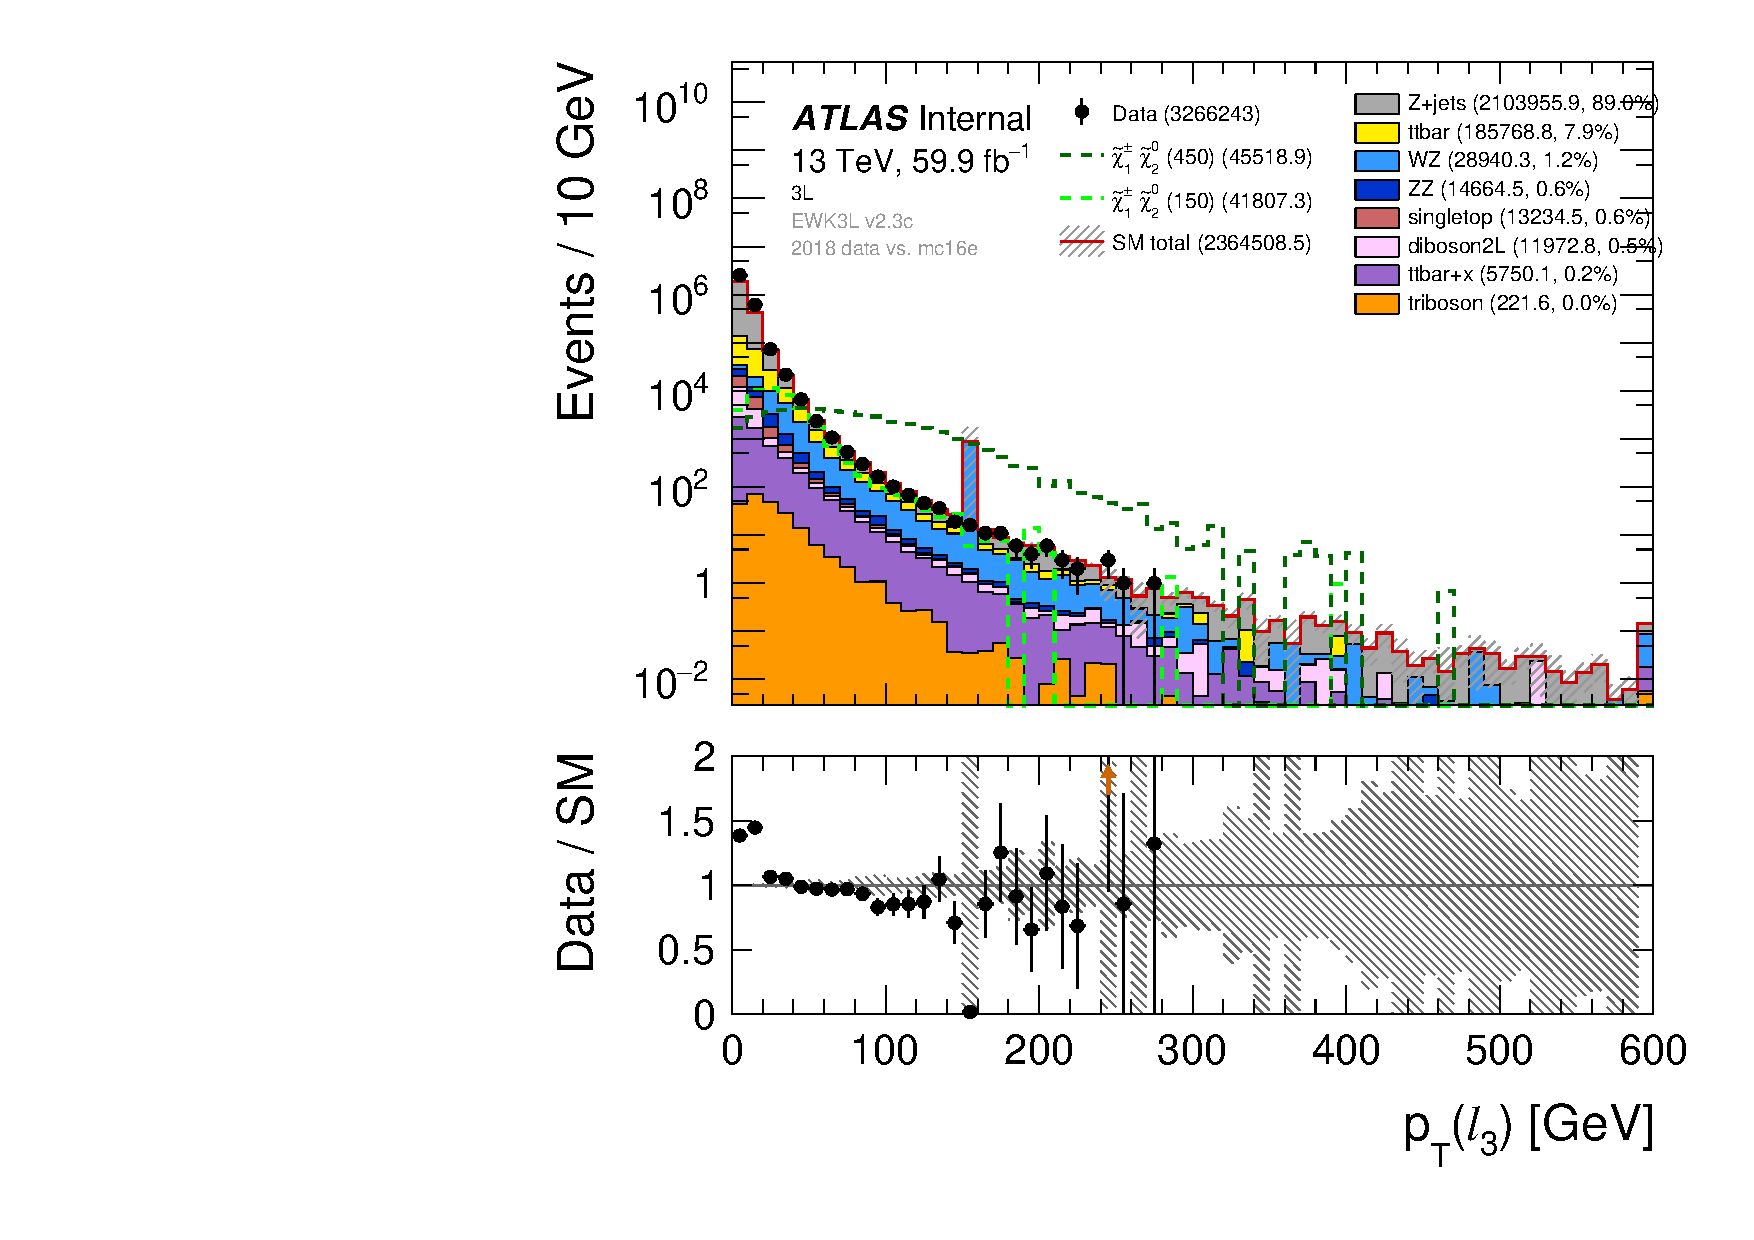
\includegraphics[width=0.55\linewidth]{ROOT_plots/hist1d_lep3Pt_3L.pdf}}
		\caption[Pt plots for the three leptons.]{Plot of the Pt of the three leptons with data, \acrshort{mc} and two neutrino signals. The number of events with higher transverse momentum decreases for each lepton, where lepton 1 has most events reaching above 800 GeV. \label{fig:Pt_orig}}
	\end{figure}

	\begin{figure}[htb!]
		\hspace*{-0.8cm}
		\subfloat[Phi neutrino]{\centering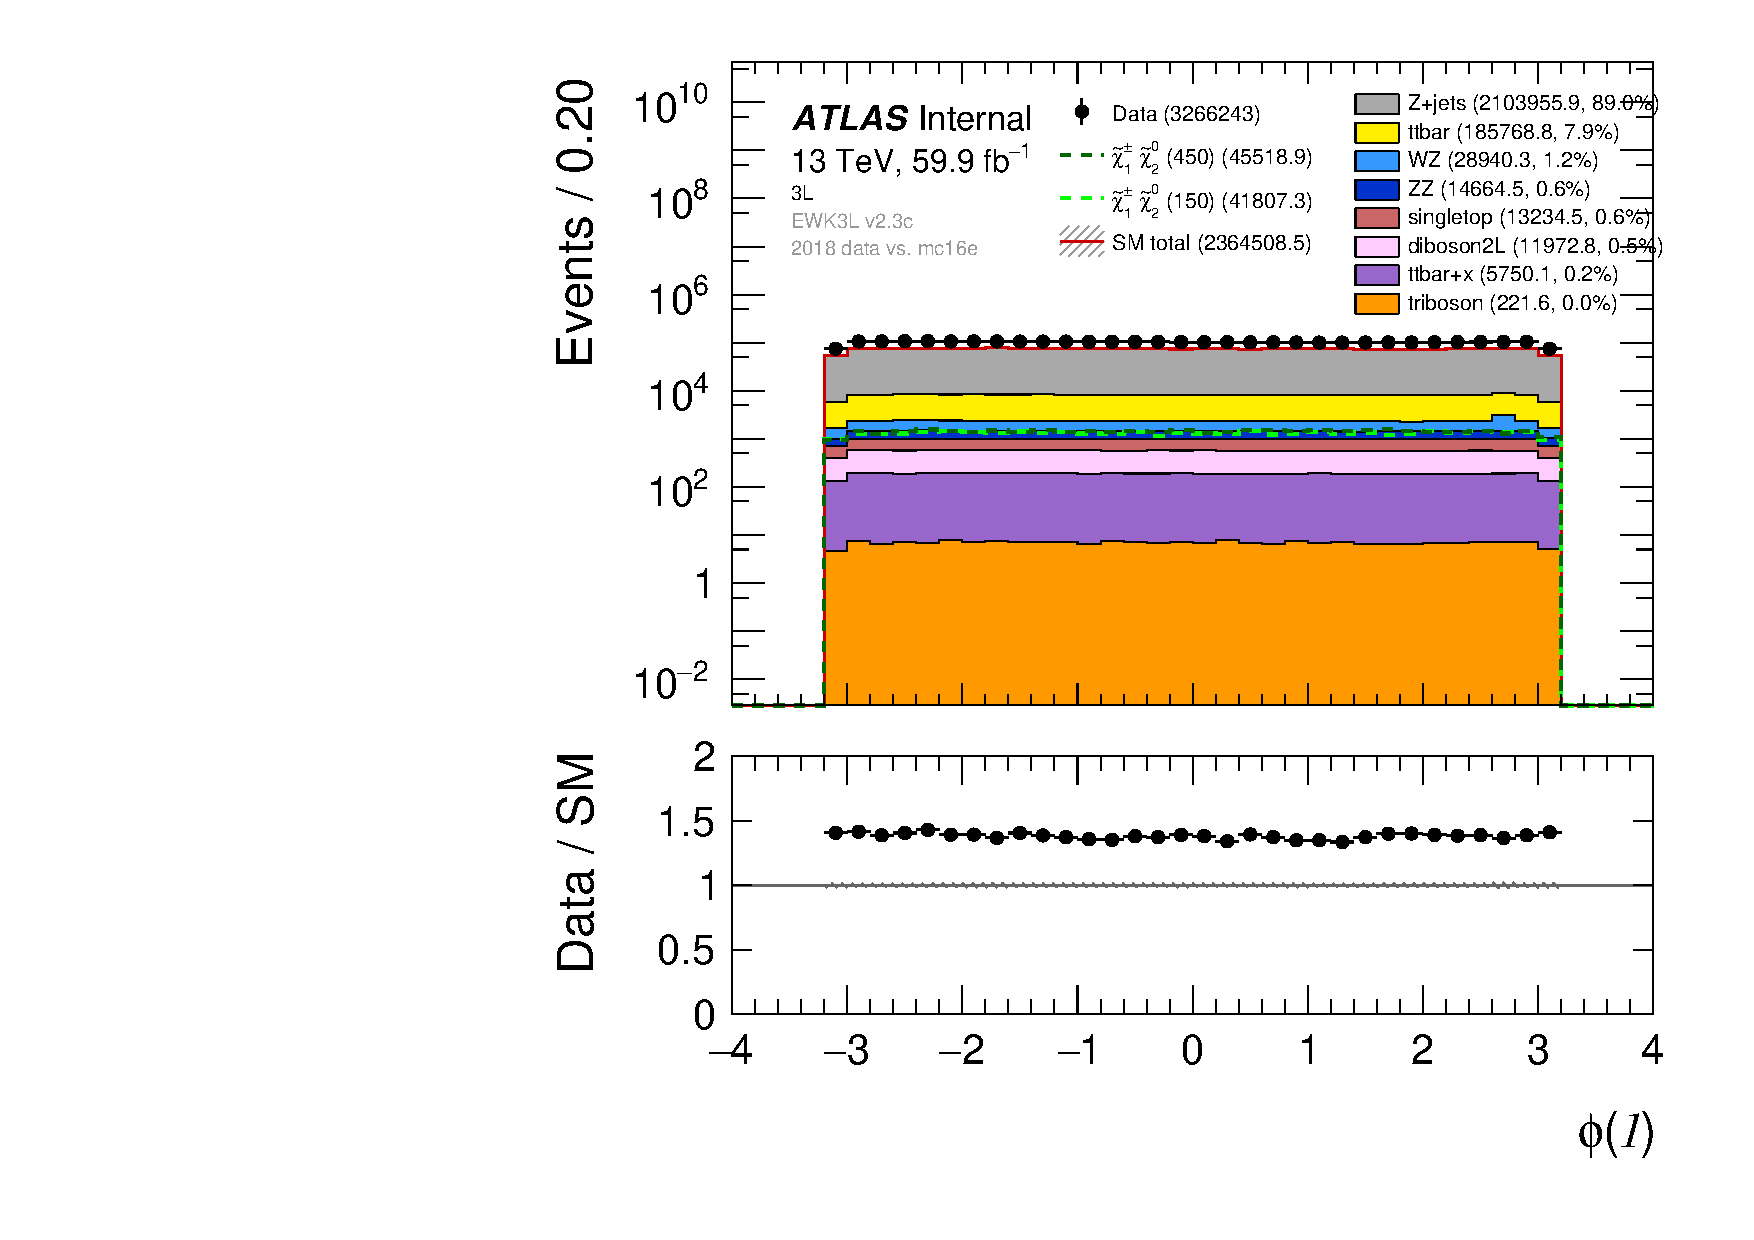
\includegraphics[width=0.55\linewidth]{ROOT_plots/hist1d_met_Phi_3L.pdf}}
		\subfloat[Missing transverse momentum]{\centering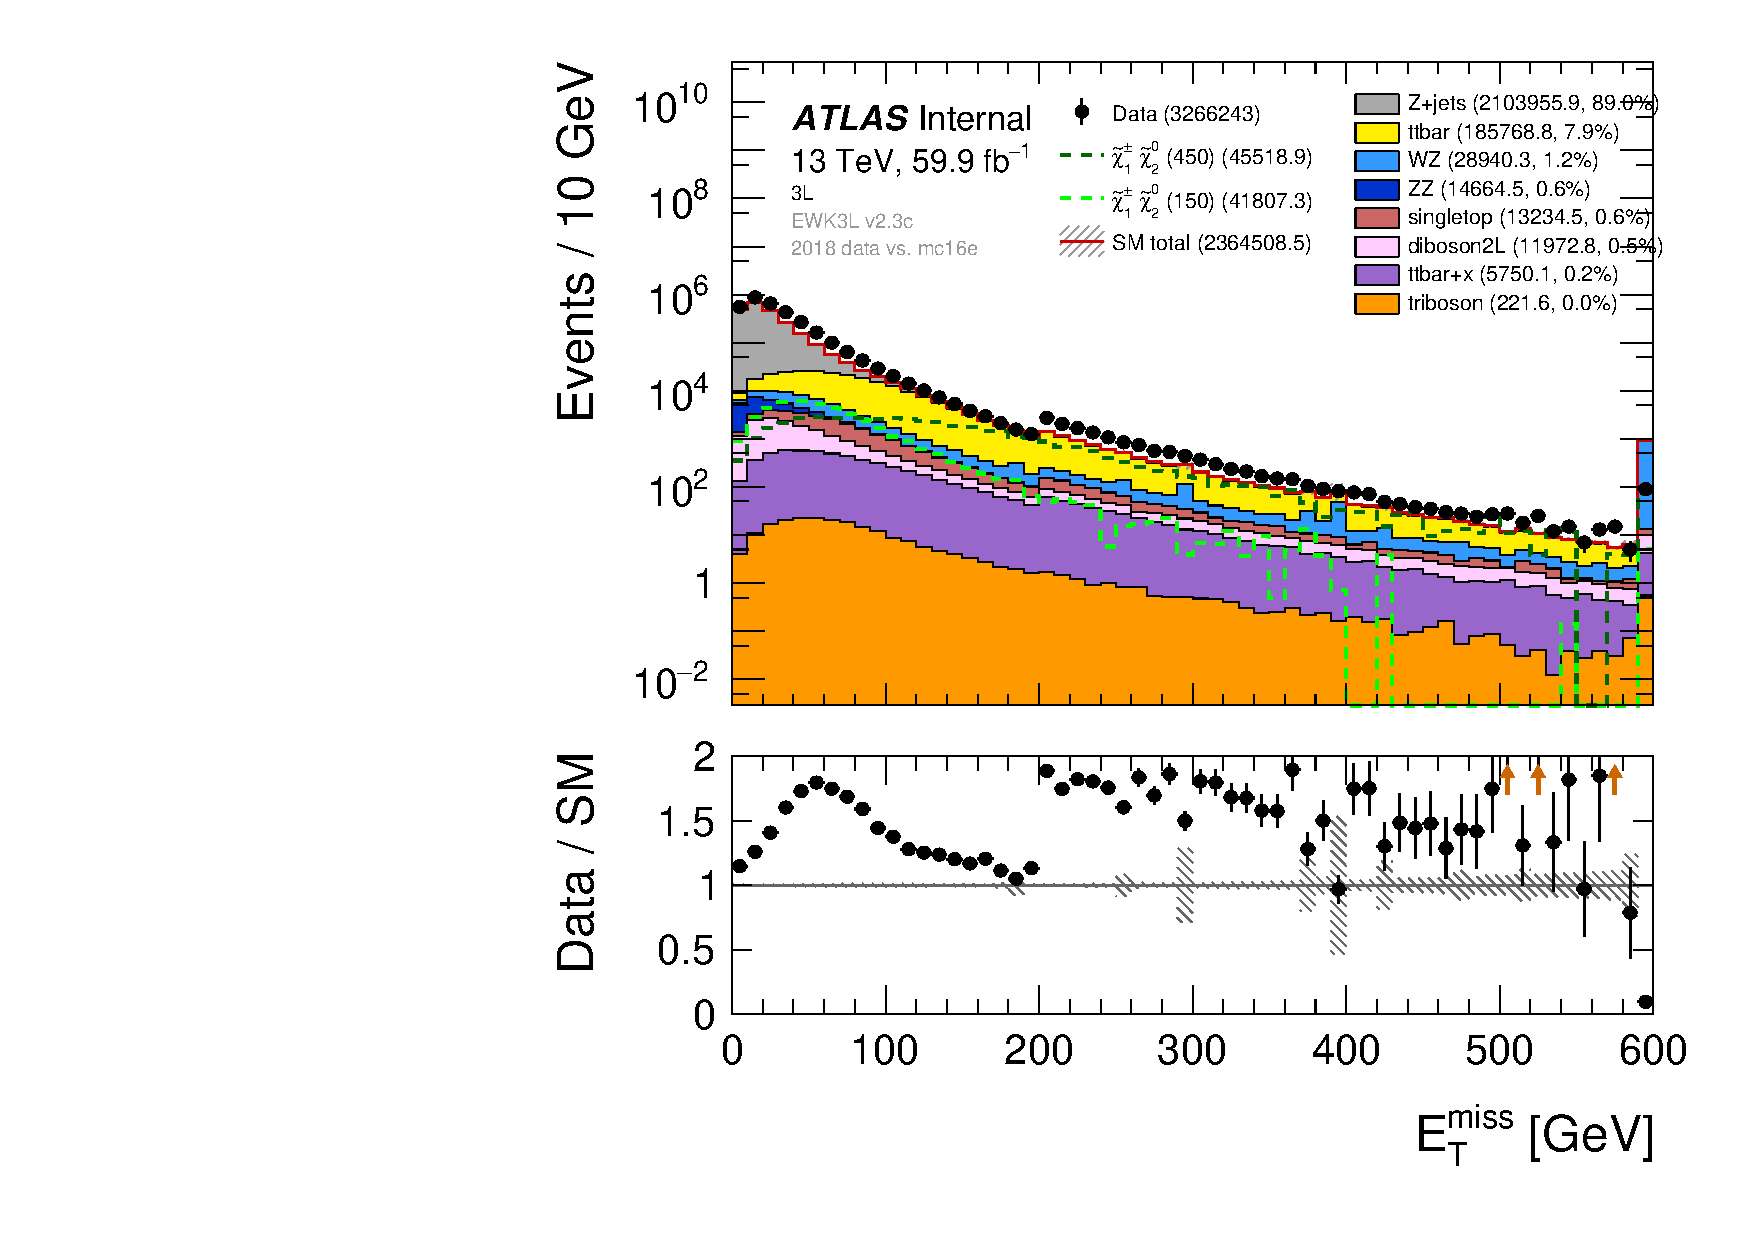
\includegraphics[width=0.55\linewidth]{ROOT_plots/hist1d_met_Et_3L.pdf}}
		\caption[Phi and missing transverse momentum plots for the neutrino.]{The figure shows the Phi and $E_t$ of the missing transverse momentum for data, \acrshort{mc} and two neutrino signals. The Phi feature is similar to the three lepton Phi features, and the \acrshort{met} is similar to the Pt feature for the leptons. \label{fig:MET_orig}}
	\end{figure}


	\section{Making New Variables}
	\label{sect:Method-MakingVariables}
	After downloading the desired data sets with the proton-proton collision events, we start by converting them from ROOT to Python syntax with the Uproot library. The files are then stored as dataframes with Pandas. This is done in the script called \textit{Trilepton\_read\_root.py}. By using the momentum and energy of the leptons in each event we compute new useful variables, which are added to a new dataframe. The new variables we make are the angular variables for each particle (three leptons and a neutrino) ($\theta$, $\phi$, $\eta$), angular variables between pairs of particles ($d\phi$, $dR$) and the invariant masses of pairs of leptons ($m_{ll}$). We also have $p_x$, $p_y$, $p_z$, $p_t$ and $E$ for all four particles. For benchmark cuts we will use later (sect. \ref{sect:Result-SRDist}), we also make a $m_{3l}$ variable for the invariant mass of the three lepton system. The new dataframes can now be imported by other scripts using Pandas to be used further with \acrshort{ml}. 
	
	The reason we make new variables for eta, phi and $p_t$ that already exists is that during the making of the invariant masses, we get some errors for some events where the $p>E$. From the Einstein energy-momentum relation in equation \ref{eq:Kinetics_Einstein}, the invariant masses becomes negative. This is not (physically) correct, and since this does not happen too often we simply drop these events in all features. This could be a simulation error, but is not known or explored in this thesis.
	
	In the Born diagram in Figure \ref{fig:ModelProcess}, the first lepton ($l_1^{\pm}$) and the pseudo-Dirac neutrino ($N$) comes from the first vertex. The second lepton ($l_2^{\mp}$) and the $W$-boson comes from the second vertex, while the third lepton ($l_3^{\pm}$) and the neutrino ($\nu$) comes from the third vertex. By using the identity traits, the particle vertex and particle ID, we classify the events by constructing a \textit{target} variable as permutations of the vertexes the leptons come from for the two signals samples we will use to train the classification models. The leptons are ordered by decreasing $p_T$, for both signals and backgrounds. The neutrino will always come from the fourth vertex in the decay chain and is not considered in the targets. This leads to the following vertex permutations for the leptons: 
	\begin{equation}
		\label{eq:Permutations}
		[123, 132, 213, 231, 312, 321]
	\end{equation}
	The function for making the new variables can be seen in Listing \ref{Lst:Making_variables}. The new dataframe is then exported as a .h5-file. 
	\begin{lstlisting}[caption=Making new variables., label=Lst:Making_variables]
		# Method for flattening and adding additional variables
		def lepaugmentation(df, nlep):
			px  = awkward.fromiter(df['px'])
			py  = awkward.fromiter(df['py'])
			pz  = awkward.fromiter(df['pz'])
			E   = awkward.fromiter(df['E'])
			vtx = awkward.fromiter(df['vtxid'])
			pid = awkward.fromiter(df['pdgid'])
		
			# Make tlv - handy when computing angular variables
			tlv = uproot_methods.classes.TLorentzVector.TLorentzVectorArray.from_cartesian(px, py, pz, E)
		
			df["tlv"] = tlv[:]
		
			df["pt"]  = tlv[:].pt
			pt  = awkward.fromiter(df['pt'])
			pt_org  = awkward.fromiter(df['pt'])
			df["phi"] = tlv[:].phi
			phi = awkward.fromiter(df['phi'])
		
			df["theta"] = tlv.theta
			theta  = awkward.fromiter(df['theta'])
		
			df["eta"] = tlv.eta
			eta  = awkward.fromiter(df['eta'])
		
			\\...
		
			# Make the lepton variables
			for i in range(1,nlep+1):
				df['lep%i_pt'%i]  = pt[pt.argmax()].flatten()
				df['lep%i_phi'%i]  = phi[pt.argmax()].flatten()
				df['lep%i_eta'%i]  = eta[pt.argmax()].flatten()
				df['lep%i_theta'%i]  = theta[pt.argmax()].flatten()
				df['lep%i_px'%i]  = px[pt.argmax()].flatten()
				df['lep%i_py'%i]  = py[pt.argmax()].flatten()
				df['lep%i_pz'%i]  = pz[pt.argmax()].flatten()
				df['lep%i_E' %i]  = E[pt.argmax()].flatten()
				df['lep%i_vtx'%i]   = vtx[pt.argmax()].flatten()
				df['lep%i_pid'%i]   = pid[pt.argmax()].flatten()
				df['lep%i_tlv'%i]   = tlv[pt.argmax()].flatten()
		
				\\...
		
		# Compute variables for all combinations of 2 leptons
		pairs = pt_org.argchoose(2)
		print("pairs:", pairs)
		left  = pairs.i0
		right = pairs.i1
		
		\\...
		
		for ilep in range(len(left[0])):
			i = left[0][ilep]
			j = right[0][ilep]
			print('i = %i, j = %i'%(i,j))
			idx1 = left[0][i]
			idx2 = right[0][i]
		
			df['mll_%i%i'%(i+1,j+1)]   = (df['lep%i_tlv'%(i+1)]+df['lep%i_tlv'%(j+1)]).apply(get_invmass)
			df['dphi_%i%i'%(i+1,j+1)] = df.apply(lambda x : get_deltaPhi(x['lep%i_tlv'%(i+1)],x['lep%i_tlv'%(j+1)]), axis=1)
			df['dR_%i%i'%(i+1,j+1)]   = df.apply(lambda x : get_deltaR(x['lep%i_tlv'%(i+1)],x['lep%i_tlv'%(j+1)]), axis=1)
		
		if Truth:
			df['target'] = df.apply(lambda x : classify_event(x['lep1_vtx'],x['lep2_vtx'],x['lep3_vtx'],x['lep4_vtx'],x['lep1_pid'],x['lep2_pid'],x['lep3_pid'],x['lep4_pid']), axis=1)
		
		
		df = df.drop(['px', 'py', 'pz', 'pt', 'E', 'vtxid', 'pdgid', 'evnum', 'onshell_w', 'tlv', 'phi', 'theta', 'eta', 'lep1_tlv', 'lep2_tlv', 'lep3_tlv', 'lep4_tlv'], axis=1)
		
		return df
	\end{lstlisting}
	
	
	\subsection{Plotting New Variables}
	\label{subsect:Method-PlottingVariables} % Rewrite
	To plot the newly produced variables, we will convert the dataframes back into ROOT to easier make similar plots like the plots we already have made. First is to convert the dataframes into comma separated values files, .csv (\acrshort{csv}), before they are converted into ROOT. In Listing \ref{Lst:CSVtoROOT} we see how we convert from \acrshort{csv} to ROOT. We only look at the \acrshort{mc} and signal data, which contain the samples of interest to us in this thesis. All plots made are found at the GitHub repository. With the new background and signal Ntuples, we can use the same plotting scripts as earlier (sect. \ref{sect:Method-Features}) to make plots of the newly produced features. 
	\begin{lstlisting}[caption=Convert from CSV to ROOT., label=Lst:CSVtoROOT]
		TFile *f = new TFile(Filename_ROOT, "RECREATE")  # Create file
		TTree *tree = new TTree(Name_of_Tree, Title_of_Tree)  # Create tree
		tree->ReadFile(Filename_CSV)  # Read the .csv-file
		tree->Fill()
		tree->Write()
	\end{lstlisting}
	
	The momentum features ($p_x$, $p_y$, $p_z$) for all four particles are seen in Figures \ref{fig:P_12} and \ref{fig:P_34}. They all have number of event peaks around 0 GeV and decreases as the absolute value of the momenta increases. $p_x$ and $p_y$ are very similar for each particle, and have events with about the same highest momentum. $p_z$ have more spiked peaks with more events with higher momentum than the other momentum coordinates. The $z$-direction is the direction the particles travel initially, which makes sense for $p_z$ to have higher momentum. The only differences between these particle momentum plots are more or less the width of the event peaks and how much momentum the events reach. Like before, lepton 1 reaches higher GeVs and decreases more and more with the other particles. The peaks also get more and more narrow for the particles.
	
	The individual angle features, $\eta$, $\theta$ and $\phi$, of the four particles are seen in Figures \ref{fig:Angular12_vars} and \ref{fig:Angular34_vars}. The $\eta$ and $\phi$ features are similar to the ones in the original Ntuples with more or less an equal amount of events for each eta and phi value, except now a peak in events around $\eta=0$ appears. $\theta$ shows similar traits like $\eta$ with equal amount of events except for a peak now around $\theta=\pi/2$.

	The transverse momentum features are seen in Figure \ref{fig:pt_all} for all four particles. They all have most events below $p_T=100$ GeV, decreasing as $p_T$ increases. Lepton 1 has most events reaching higher $p_T$ values around 800 GeV, while the neutrino with smallest $p_T$s has only most events reaching $p_T$ around 400 GeV. The $E$ features in Figure \ref{fig:E_m3l} show the same type of behavior like the $p_T$ features, where lepton 1 has much higher energy than the other particles and it decreases more and more for each particle. Lepton 1 has events reaching around 1 TeV, while the neutrino only has events reaching around 200 GeV. The invariant mass of the three lepton system is similar to the lepton 1 energy, reaching around 1 TeV for all backgrounds. The 450 GeV signal has more events for higher mass $>450$ GeV, while the 150 GeV signal has more events for lower masses.
	
	The invariant mass pair plots in Figure \ref{fig:mll_vars} look similar to the transverse momentum plots, where the event peaks are between 0 and 100 GeV depending on the particle combinations, and decreases as the invariant masses increases. The 150 GeV signal follows the \acrshort{mc} for the number of events while the 450 GeV signal first reaches the peak around 400 GeV for the more massive combinations. 
	
	The azimuthal angle difference between pairs of particles are seen in Figure \ref{fig:dPhi_vars}. Most of the pairs have small peaks around $\Delta\phi=\pm\pi$ and $\Delta\phi=0$ with not much difference in the number of events elsewhere. The two signals have fewer events around $\Delta\phi=0$, especially for the lepton 1 and 2 and 1 and 3 pairs.
	
	The angular distance features for all four particles in Figure \ref{fig:dR_vars} have the number of events increasing slowly until the angular distance is around 3.2 before it decreases more rapidly when the angular distance approaches 6. This happens for all combinations of angular distances. The main differences is how steep the increase and decrease are when the angular distance approaches 3.2 and 6, respectively. 
	% px,py,pz
	\begin{figure}[h!]
		\vspace*{-4.5cm}
		\hspace*{-1.cm}
		\subfloat[$p_x$ lepton 1\label{subfig:Px1}]{\centering\includegraphics[width=0.55\linewidth]{Feature_plots/hist1d_lep1_px_SR_3L.pdf}}
		\subfloat[$p_x$ lepton 2\label{subfig:Px2}]{\centering\includegraphics[width=0.55\linewidth]{Feature_plots/hist1d_lep2_px_SR_3L.pdf}}\\
		\hspace*{-1.cm}
		\subfloat[$p_y$ lepton 1\label{subfig:Py1}]{\centering\includegraphics[width=0.55\linewidth]{Feature_plots/hist1d_lep1_py_SR_3L.pdf}}
		\subfloat[$p_y$ lepton 2\label{subfig:Py2}]{\centering\includegraphics[width=0.55\linewidth]{Feature_plots/hist1d_lep2_py_SR_3L.pdf}}\\
		\hspace*{-1.cm}
		\subfloat[$p_z$ lepton 1\label{subfig:Pz1}]{\centering\includegraphics[width=0.55\linewidth]{Feature_plots/hist1d_lep1_pz_SR_3L.pdf}}
		\subfloat[$p_z$ lepton 2\label{subfig:Pz2}]{\centering\includegraphics[width=0.55\linewidth]{Feature_plots/hist1d_lep2_pz_SR_3L.pdf}}
		\caption[The momentum for lepton 1 and 2.]{The momentum features of lepton 1 and 2. They both have number of event peaks around 0 GeV, but lepton 1 has a broader peak reach higher (absolute) energies. \label{fig:P_12}}
	\end{figure}
	\begin{figure}[h!]
		\vspace*{-4.5cm}
		\hspace*{-1.cm}
		\subfloat[$p_x$ lepton 3\label{subfig:Px3}]{\centering\includegraphics[width=0.55\linewidth]{Feature_plots/hist1d_lep3_px_SR_3L.pdf}}
		\subfloat[$p_x$ lepton 4\label{subfig:Px4}]{\centering\includegraphics[width=0.55\linewidth]{Feature_plots/hist1d_lep4_px_SR_3L.pdf}}\\
		\hspace*{-1.cm}
		\subfloat[$p_y$ lepton 3\label{subfig:Py3}]{\centering\includegraphics[width=0.55\linewidth]{Feature_plots/hist1d_lep3_py_SR_3L.pdf}}
		\subfloat[$p_y$ lepton 4\label{subfig:Py4}]{\centering\includegraphics[width=0.55\linewidth]{Feature_plots/hist1d_lep4_py_SR_3L.pdf}}\\
		\hspace*{-1.cm}
		\subfloat[$p_z$ lepton 3\label{subfig:Pz3}]{\centering\includegraphics[width=0.55\linewidth]{Feature_plots/hist1d_lep3_pz_SR_3L.pdf}}
		\subfloat[$p_z$ lepton 4\label{subfig:Pz4}]{\centering\includegraphics[width=0.55\linewidth]{Feature_plots/hist1d_lep4_pz_SR_3L.pdf}}
		\caption[The momentum for lepton 3 and the neutrino.]{The momentum features of lepton 3 and the neutrino. These plots are similar to lepton 1 and 2, except for the lower highest momentum for the events. \label{fig:P_34}}
	\end{figure}

	%theta,eta,phi
	\begin{figure}[h!]
		\vspace*{-4.5cm}
		\hspace*{-1.cm}
		\subfloat[$\theta$ lepton 1\label{subfig:Theta1}]{\centering\includegraphics[width=0.55\linewidth]{Feature_plots/hist1d_lep1_theta_SR_3L.pdf}}
		\subfloat[$\theta$ lepton 2\label{subfig:Theta2}]{\centering\includegraphics[width=0.55\linewidth]{Feature_plots/hist1d_lep2_theta_SR_3L.pdf}}\\
		\hspace*{-1.cm}
		\subfloat[$\eta$ lepton 1\label{subfig:Eta11}]{\centering\includegraphics[width=0.55\linewidth]{Feature_plots/hist1d_lep1_eta_SR_3L.pdf}}
		\subfloat[$\eta$ lepton 2\label{subfig:Eta22}]{\centering\includegraphics[width=0.55\linewidth]{Feature_plots/hist1d_lep2_eta_SR_3L.pdf}}\\
		\hspace*{-1.cm}
		\subfloat[$\phi$ lepton 1\label{subfig:Phi11}]{\centering\includegraphics[width=0.55\linewidth]{Feature_plots/hist1d_lep1_phi_SR_3L.pdf}}
		\subfloat[$\phi$ lepton 2\label{subfig:Phi22}]{\centering\includegraphics[width=0.55\linewidth]{Feature_plots/hist1d_lep2_phi_SR_3L.pdf}}
		\caption[The angular features for lepton 1 and 2.]{The angular features ($\theta$, $\eta$, $\phi$) for lepton 1 and 2. Almost all the angular values have an equal amount of events, except for $\theta$ with a peak around $\theta=\pi/2$ and $\eta$ with a peak around $\eta=0$. \label{fig:Angular12_vars}}
	\end{figure}
	\begin{figure}[h!]
		\vspace*{-4.5cm}
		\hspace*{-1.cm}
		\subfloat[$\theta$ lepton 3\label{subfig:Theta3}]{\centering\includegraphics[width=0.55\linewidth]{Feature_plots/hist1d_lep3_theta_SR_3L.pdf}}
		\subfloat[$\theta$ lepton 4\label{subfig:Theta4}]{\centering\includegraphics[width=0.55\linewidth]{Feature_plots/hist1d_lep4_theta_SR_3L.pdf}}\\
		\hspace*{-1.cm}
		\subfloat[$\eta$ lepton 3\label{subfig:Eta33}]{\centering\includegraphics[width=0.55\linewidth]{Feature_plots/hist1d_lep3_eta_SR_3L.pdf}}
		\subfloat[$\eta$ lepton 4\label{subfig:Eta44}]{\centering\includegraphics[width=0.55\linewidth]{Feature_plots/hist1d_lep4_eta_SR_3L.pdf}}\\
		\hspace*{-1.cm}
		\subfloat[$\phi$ lepton 3\label{subfig:Phi33}]{\centering\includegraphics[width=0.55\linewidth]{Feature_plots/hist1d_lep3_phi_SR_3L.pdf}}
		\subfloat[$\phi$ lepton 4\label{subfig:Phi44}]{\centering\includegraphics[width=0.55\linewidth]{Feature_plots/hist1d_lep4_phi_SR_3L.pdf}}
		\caption[The angular features for lepton 3 and the neutrino.]{The angular features ($\theta$, $\eta$, $\phi$) for lepton 3 and the neutrino. Almost all the angular values have an equal amount of events, except for $\theta$ with a peak around $\theta=\pi/2$ and $\eta$ with a peak around $\eta=0$. \label{fig:Angular34_vars}}
	\end{figure}

	%pt
	\begin{figure}[h!]
		\vspace*{-4.5cm}
		\hspace*{-1.cm}
		\subfloat[$p_T$ lepton 1\label{subfig:pt1}]{\centering\includegraphics[width=0.55\linewidth]{Feature_plots/hist1d_lep1_pt_SR_3L.pdf}}
		\subfloat[$p_T$ lepton 2\label{subfig:pt2}]{\centering\includegraphics[width=0.55\linewidth]{Feature_plots/hist1d_lep2_pt_SR_3L.pdf}}\\
		\hspace*{-1.cm}
		\subfloat[$p_T$ lepton 3\label{subfig:pt31}]{\centering\includegraphics[width=0.55\linewidth]{Feature_plots/hist1d_lep3_pt_SR_3L.pdf}}
		\subfloat[$p_T$ lepton 4\label{subfig:pt42}]{\centering\includegraphics[width=0.55\linewidth]{Feature_plots/hist1d_lep4_pt_SR_3L.pdf}}\\
		\caption[$p_T$ for all three leptons and neutrino.]{The transverse momentum for all four particles showing decreasing number of events when the momenta increases. Lepton 1 has events reaching highest $p_T$ around 800 GeV. \label{fig:pt_all}}
	\end{figure}

	%E, m3l
	\begin{figure}[h!]
		\vspace*{-4.5cm}
		\hspace*{-1.cm}
		\subfloat[$E$ lepton 1\label{subfig:E1}]{\centering\includegraphics[width=0.55\linewidth]{Feature_plots/hist1d_lep1_E_SR_3L.pdf}}
		\subfloat[$E$ lepton 2\label{subfig:E2}]{\centering\includegraphics[width=0.55\linewidth]{Feature_plots/hist1d_lep2_E_SR_3L.pdf}}\\
		\hspace*{-1.cm}
		\subfloat[$E$ lepton 3\label{subfig:E3}]{\centering\includegraphics[width=0.55\linewidth]{Feature_plots/hist1d_lep3_E_SR_3L.pdf}}
		\subfloat[$E$ lepton 4\label{subfig:E4}]{\centering\includegraphics[width=0.55\linewidth]{Feature_plots/hist1d_lep4_E_SR_3L.pdf}}\\
		\hspace*{3.cm}
		\subfloat[Invariant mass of three lepton system\label{subfig:m3l}]{\centering\includegraphics[width=0.55\linewidth]{Feature_plots/hist1d_m_3l_SR_3L.pdf}}
		\caption[$E$ for all particles and $m_{3l}$ for the three lepton system.]{Energy for all particles in Figures \ref{subfig:E1} to \ref{subfig:E4}, and the invariant mass for the three lepton system in \ref{subfig:m3l}. Similar behavior for lepton 1 and invariant mass with high amount of events reaching around 1 TeV. \label{fig:E_m3l}}
	\end{figure}

	% mll
	\begin{figure}[h!]
		\vspace*{-4.5cm}
		\hspace*{-1.cm}
		\subfloat[$m_{ll}$ lepton 1 and 2\label{subfig:mll12}]{\centering\includegraphics[width=0.55\linewidth]{Feature_plots/hist1d_mll_12_SR_3L.pdf}}
		\subfloat[$m_{ll}$ lepton 1 and 3\label{subfig:mll13}]{\centering\includegraphics[width=0.55\linewidth]{Feature_plots/hist1d_mll_13_SR_3L.pdf}}\\
		\hspace*{-1.cm}
		\subfloat[$m_{ll}$ lepton 1 and neutrino\label{subfig:mll14}]{\centering\includegraphics[width=0.55\linewidth]{Feature_plots/hist1d_mll_14_SR_3L.pdf}}
		\subfloat[$m_{ll}$ lepton 2 and 3\label{subfig:mll23}]{\centering\includegraphics[width=0.55\linewidth]{Feature_plots/hist1d_mll_23_SR_3L.pdf}}\\
		\hspace*{-1.cm}
		\subfloat[$m_{ll}$ lepton 2 and neutrino\label{subfig:mll24}]{\centering\includegraphics[width=0.55\linewidth]{Feature_plots/hist1d_mll_24_SR_3L.pdf}}
		\subfloat[$m_{ll}$ lepton 3 and neutrino\label{subfig:mll34}]{\centering\includegraphics[width=0.55\linewidth]{Feature_plots/hist1d_mll_34_SR_3L.pdf}}
		\caption[Invariant masses between pairs of particles.]{Invariant masses between pairs of particles. The further out in the vertices the particles appear, the less is the invariant mass of the combinations of those particles. \label{fig:mll_vars}}
	\end{figure}

	% dPhi
	\begin{figure}[h!]
		\vspace*{-4.5cm}
		\hspace*{-1.cm}
		\subfloat[$\Delta \phi$ lepton 1 and 2\label{subfig:dPhi12}]{\centering\includegraphics[width=0.55\linewidth]{Feature_plots/hist1d_dphi_12_SR_3L.pdf}}
		\subfloat[$\Delta \phi$ lepton 1 and 3\label{subfig:dPhi13}]{\centering\includegraphics[width=0.55\linewidth]{Feature_plots/hist1d_dphi_13_SR_3L.pdf}}\\
		\hspace*{-1.cm}
		\subfloat[$\Delta \phi$ lepton 1 and neutrino\label{subfig:dPhi14}]{\centering\includegraphics[width=0.55\linewidth]{Feature_plots/hist1d_dphi_14_SR_3L.pdf}}
		\subfloat[$\Delta \phi$ lepton 2 and 3\label{subfig:dPhi23}]{\centering\includegraphics[width=0.55\linewidth]{Feature_plots/hist1d_dphi_23_SR_3L.pdf}}\\
		\hspace*{-1.cm}
		\subfloat[$\Delta \phi$ lepton 2 and neutrino\label{subfig:dPhi24}]{\centering\includegraphics[width=0.55\linewidth]{Feature_plots/hist1d_dphi_24_SR_3L.pdf}}
		\subfloat[$\Delta \phi$ lepton 3 and neutrino\label{subfig:dPhi34}]{\centering\includegraphics[width=0.55\linewidth]{Feature_plots/hist1d_dphi_34_SR_3L.pdf}}
		\caption[The azimuthal angular difference features between pairs of particles.]{The azimuthal angular difference features between pairs of particles. Most of the combinations have small peaks around $\Delta\phi=\pm\pi$ and $\Delta\phi=0$. \label{fig:dPhi_vars}}
	\end{figure}

	% dR
	\begin{figure}[h!]
		\vspace*{-4.5cm}
		\hspace*{-1.cm}
		\subfloat[$\Delta$R lepton 1 and 2\label{subfig:dR12}]{\centering\includegraphics[width=0.55\linewidth]{Feature_plots/hist1d_dR_12_SR_3L.pdf}}
		\subfloat[$\Delta$R lepton 1 and 3\label{subfig:dR13}]{\centering\includegraphics[width=0.55\linewidth]{Feature_plots/hist1d_dR_13_SR_3L.pdf}}\\
		\hspace*{-1.cm}
		\subfloat[$\Delta$R lepton 1 and neutrino\label{subfig:dR14}]{\centering\includegraphics[width=0.55\linewidth]{Feature_plots/hist1d_dR_14_SR_3L.pdf}}
		\subfloat[$\Delta$R lepton 2 and 3\label{subfig:dR23}]{\centering\includegraphics[width=0.55\linewidth]{Feature_plots/hist1d_dR_23_SR_3L.pdf}}\\
		\hspace*{-1.cm}
		\subfloat[$\Delta$R lepton 2 and neutrino\label{subfig:dR24}]{\centering\includegraphics[width=0.55\linewidth]{Feature_plots/hist1d_dR_24_SR_3L.pdf}}
		\subfloat[$\Delta$R lepton 3 and neutrino\label{subfig:dR34}]{\centering\includegraphics[width=0.55\linewidth]{Feature_plots/hist1d_dR_34_SR_3L.pdf}}
		\caption[The angular distance features between pairs of particles.]{The angular distance features between pairs of particles. The number of events increase mostly as $\Delta R$ approaches 3.2, and the decreases as $\Delta R$ approaches 6. \label{fig:dR_vars}}
	\end{figure}
	
	

%----------------------------------------------------------------------	

	\chapter{Evaluation of ML Models}
	\label{chap:Method-DataPrep}
	
	
	\section{Preprocessing of the Data}
	\label{sect:Method-PrepData}
	After importing all the necessary libraries in a new script, \textit{Trilepton\_classifier.py}, we load in the dataframes and drop unnecessary features and events we will not consider in the classification. With some useful properties of Pandas dataframes, and utilizing Seaborn and Scikit-Learn, we need to do some preprocessing of the data. One thing we have to consider for our data set is NaN, or NULL, values. Not all classification models can deal with NaN values, so these have to be dealt with. We can check for NaN values and drop them easily from the dataframe by doing the following in Listing \ref{Lst:NULL_check}:
	\begin{lstlisting}[caption=Check NULL values., label=Lst:NULL_check]
		df.isnull()   # Returns a boolean matrix, if the value is NaN then True otherwise False.
		df.isnull().sum()   # Returns the column names along with the number of NaN values in that particular column.
		df.dropna(inplace=True)  # Removes rows in the dataframe containing NaN values.
	\end{lstlisting}


	\subsection{Inspect Data}
	\label{subsect:Method-Inspect Data}
	Pandas dataframes lets us easily print a few lines and a summary of the dataframe. We then get a quick overview of what the data looks like. The $N1=150$ GeV data summary:
	\begin{lstlisting}[caption=Inspect data.,label=InspectData]
		<class 'pandas.core.frame.DataFrame'>
		Int64Index: 66885 entries, 0 to 67773
		Data columns (total 55 columns):
		 #   Column      Non-Null Count  Dtype
		---  ------      --------------  -----
		 0   lep1_pt     66885 non-null  float32
		 1   lep1_phi    66885 non-null  float32
		 2   lep1_eta    66885 non-null  float32
		 3   lep1_theta  66885 non-null  float32
		 4   lep1_px     66885 non-null  float32
		 5   lep1_py     66885 non-null  float32
		 6   lep1_pz     66885 non-null  float32
		 7   lep1_E      66885 non-null  float32
		 8   lep1_tlv    66885 non-null  object
		 9   lep2_pt     66885 non-null  float32
		 10  lep2_phi    66885 non-null  float32
		 11  lep2_eta    66885 non-null  float32
		 12  lep2_theta  66885 non-null  float32
		 13  lep2_px     66885 non-null  float32
		 14  lep2_py     66885 non-null  float32
		 15  lep2_pz     66885 non-null  float32
		 16  lep2_E      66885 non-null  float32
		 17  lep2_tlv    66885 non-null  object
		 18  lep3_pt     66885 non-null  float32
		 19  lep3_phi    66885 non-null  float32
		 20  lep3_eta    66885 non-null  float32
		 21  lep3_theta  66885 non-null  float32
		 22  lep3_px     66885 non-null  float32
		 23  lep3_py     66885 non-null  float32
		 24  lep3_pz     66885 non-null  float32
		 25  lep3_E      66885 non-null  float32
		 26  lep3_tlv    66885 non-null  object
		 27  lep4_pt     66885 non-null  float32
		 28  lep4_phi    66885 non-null  float32
		 29  lep4_eta    66885 non-null  float32
		 30  lep4_theta  66885 non-null  float32
		 31  lep4_px     66885 non-null  float32
		 32  lep4_py     66885 non-null  float32
		 33  lep4_pz     66885 non-null  float32
		 34  lep4_E      66885 non-null  float32
		 35  lep4_tlv    66885 non-null  object
		 36  mll_12      66885 non-null  float64
		 37  dphi_12     66885 non-null  float64
		 38  dR_12       66885 non-null  float64
		 39  mll_13      66885 non-null  float64
		 40  dphi_13     66885 non-null  float64
		 41  dR_13       66885 non-null  float64
		 42  mll_23      66885 non-null  float64
		 43  dphi_23     66885 non-null  float64
		 44  dR_23       66885 non-null  float64
		 45  mll_14      66885 non-null  float64
		 46  dphi_14     66885 non-null  float64
		 47  dR_14       66885 non-null  float64
		 48  mll_24      66885 non-null  float64
		 49  dphi_24     66885 non-null  float64
		 50  dR_24       66885 non-null  float64
		 51  mll_34      66885 non-null  float64
		 52  dphi_34     66885 non-null  float64
		 53  dR_34       66885 non-null  float64
		 54  target      66885 non-null  object
		dtypes: float32(32), float64(18), object(5)
		memory usage: 20.4+ MB
		
					 lep1_pt  lep1_phi  lep1_eta  ...   dphi_34     dR_34 target
		entry                                     ...
		0      364078.281250  1.312494 -1.321615  ...  0.891000  0.892144  			(1, 2, 3)
		2       43565.238281  1.124601  1.340168  ...  2.664658  3.030723  			(1, 3, 2)
		3       62504.234375 -3.002433 -0.343577  ...  0.209667  1.262884  			(3, 2, 1)
		4       77743.296875 -1.776769 -1.809337  ... -2.731673  3.427304  			(2, 3, 1)
		5       65388.453125  2.266318  2.015514  ...  2.228343  2.480432  			(1, 2, 3)
		
		[5 rows x 55 columns]
	\end{lstlisting}
	The data summary for the $N1=450$ GeV signal can be found in Appendix \ref{appendix:Signal450_Summary}. The two data summaries are very similar, but the 450 GeV signal has more events. The prints show short looks at the features in the dataframes, like the values for a few events, the names and index dtypes of each feature in the dataframes. They also count and print the number of non-null values and the memory usage. 
	
	Then we make a design matrix \textbf{X}, containing all the variables for each event, and a target vector \textbf{Y}, containing all the targets for each event. The targets are at this point of type \textit{tuples}. This makes classification more difficult, which is why we convert each event target in \textbf{Y} into an \textit{integer} and make a new target vector \textbf{y} with the different vertex permutations as in equation \ref{eq:Permutations}. 
	
	Another useful thing to print is the individual target counts in the target vector \textbf{y} to check the number of each target in the dataframe. With this check, we quickly get an overview to see if we have a balanced or imbalanced data set. This can be very important to check, since it might lead to problems later. The target counts for both signals are seen in Table \ref{tab:Counts_original}. We easily see that there is an imbalance in both the data sets, and that the 450 GeV signal has a lot more events. Vertex permutation 123 has the highest count for the 150 GeV signal, which is where the highest $p_T$ comes from the $N_1$ production vertex. For the 450 GeV signal 231 hs the highest count, which corresponds to the case where the highest $p_T$ comes from the $N_1$ decay. The second highest comes from the final $W$, and the third highest comes from the $N_1$ production vertex. When the mass of $N_1$ is large,450 GeV, a lot of momentum is released into the lepton when it decays. When $N_1$ is small, 150 GeV, the first lepton has more phase space and thus can typically have larger momentum.
	\begin{table}[htbp!]
		\centering
		%\hspace{-1cm}
		\begin{tabular}{ |c|c|c| }
			\hline
			\multirow{2}{*}{Vertex permutations} & \multicolumn{2}{|c|}{$N1$}\\
			\cline{2-3} \rule{0pt}{13pt}
			 & 150 GeV & 450 GeV  \\
			\hline \rule{0pt}{13pt}
			123 & 26801 & 34303 \\
			\hline \rule{0pt}{13pt}
			132 & 9716 & 10863 \\
			\hline \rule{0pt}{13pt}
			213 & 12871 & 65308 \\
			\hline \rule{0pt}{13pt}
			231 & 8454 & 139686 \\
			\hline \rule{0pt}{13pt}
			312 & 4013 & 3938 \\
			\hline \rule{0pt}{13pt}
			321 & 5030 & 5338 \\
			\hline
		\end{tabular}	
		\caption[Target counts of the classes.]{The target counts for both signal samples. For the 150 GeV signal, the highest target counts is for vertex permutation 123. For the 450 GeV signal, 231 has the highest count.}
		\label{tab:Counts_original}
	\end{table}
	
	
	\subsubsection{Correlations}
	\label{subsubsect:Method-Correlations}
	An important descriptive statistic for data analysis with multi-variable data is the \textit{correlation matrix} using Seaborn. It is a symmetric table of size $k\times k$, for $k$ features (this includes the targets as well), with pairwise correlations between the features in the data. It summarizes the relationships between the features that we most likely would not have seen by just looking at them. With machine learning, it is also an early preprocessing step that can give some information to whereas dimensionality reduction might come in handy when dealing with high-dimensionality data. The closer to 1 the correlation coefficients are, the more correlated are they. We don't want a value close to -1, since this indicates a strong negative correlation. The diagonal will of course always be 1, since it is the correlation between the feature itself. When a feature has a strong correlation to the target, it has a higher significance for predicting the output than a feature close to -1. This helps us exclude features that worsen the predictions. The optimal case is then a high positive correlation between the independent and dependent variables, while any strong correlation between the independent variables (causing redundancy) is not.
	
	By using the correlations between the features, we print the feature pairs with strong correlation (magnitude greater than 0.7) for the $N1=150$ GeV signal:
	\begin{lstlisting}[caption=Feature correlation 150 GeV signal,label=Feature150]
		lep1_theta  lep1_eta     -0.982589
		lep2_theta  lep2_eta     -0.980482
		lep3_eta    lep3_theta   -0.979638
		lep4_eta    lep4_theta   -0.967329
		lep2_py     lep1_py      -0.861290
		lep2_px     lep1_px      -0.832358
		lep1_pz     lep1_theta   -0.821220
		lep2_pz     lep2_theta   -0.798809
		lep3_theta  lep3_pz      -0.788853
		lep4_pz     lep4_theta   -0.701025
		lep3_phi    lep3_py       0.707593
		lep1_pt     lep3_pt       0.712439
		mll_13      lep2_pt       0.719664
					lep3_pt       0.753440
		mll_12      mll_13        0.784307
		lep4_pz     lep4_eta      0.812571
		lep1_pt     mll_13        0.827285
		lep2_pz     lep2_eta      0.863876
		lep3_eta    lep3_pz       0.868294
		lep1_pz     lep1_eta      0.872948
		lep1_pt     mll_12        0.900048
		mll_12      lep2_pt       0.900361
		lep2_pt     lep1_pt       0.914949
	\end{lstlisting}
	We print the same for the 450 GeV signal yielding similar results:
	\begin{lstlisting}[caption=Feature correlation 450 GeV signal.,label=Feature450]
		lep1_eta    lep1_theta   -0.991685
		lep4_eta    lep4_theta   -0.987881
		lep3_eta    lep3_theta   -0.984183
		lep2_eta    lep2_theta   -0.984020
		lep1_pz     lep1_theta   -0.894602
		lep1_py     lep2_py      -0.890322
		lep2_px     lep1_px      -0.851323
		lep2_pz     lep2_theta   -0.849920
		lep3_pz     lep3_theta   -0.805985
		lep4_theta  lep4_pz      -0.778867
		dR_14       dR_13        -0.759559
		dR_13       dR_23        -0.715678
					dphi_23      -0.709584
		lep2_py     lep1_phi     -0.707875
		lep4_phi    lep4_py       0.704739
		lep3_py     lep3_phi      0.718642
		dR_24       mll_24        0.730663
		lep2_py     lep2_phi      0.735340
		lep3_pt     mll_13        0.752684
		mll_14      dR_14         0.775010
		lep1_phi    lep1_py       0.783622
		dphi_23     dphi_12       0.783714
		dR_13       mll_13        0.805792
		lep4_eta    lep4_pz       0.806726
		lep1_pt     lep2_pt       0.850018
		mll_12      lep1_pt       0.862141
					lep2_pt       0.864872
		lep3_pz     lep3_eta      0.872818
		lep2_pz     lep2_eta      0.898086
		lep1_pz     lep1_eta      0.924052
	\end{lstlisting} 
	The features we have printed for the two signals shows features that have strong correlations, either positive or negative correlations, between the pairs. These feature correlations may affect the predictions and is something we do not want. For this reason we may want to remove some of these features. The full correlation matrices can be seen in Figures \textit{Correlation\_150.png} and \textit{Correlation\_450.png} in the \textbf{Plots}-folder at the GitHub repository. 
		
	To take a closer look at the correlations in the data set, we use the mutual information of the features from section \ref{subsect:Theory-MutualInfo}. By using the \textit{mutual\_info\_classif} function by Scikit-Learn, we can easily compute the information gain of the features and the targets. We want the features that maximizes the information gain. This helps us single out unnecessary features for classification. The full information gains for all features can be seen in Appendix \ref{appendix:Correlations}.
	
	From the strong correlation pairs, correlation matrices and the mutual information we choose to remove the eta features for all the four particles (lep(1,2,3,4)\_eta) in both signals since they show high correlations to other features and have low mutual information, as seen in Table \ref{tab:MutualInfo_eta}. lep1\_pt shows a high correlation with other features, but has one of the highest values for mutual information with the target, lep1\_pt $\approx 0.2766$ for the 150 GeV signal. This is why we do not remove it. In the case of decision trees, the information gain is used for the splitting in the trees.
	\begin{table}[htbp!]
		\centering
		%\hspace{-1cm}
		\begin{tabular}{ |c|c|c| }
			\hline \rule{0pt}{13pt}
			$N1$ & 150 GeV  & 450 GeV   \\
			\hline \rule{0pt}{13pt}
			lep1\_eta & 0.0617 & 0.4363 \\
			\hline \rule{0pt}{13pt}
			lep2\_eta & 0.0604 & 0.4218  \\
			\hline \rule{0pt}{13pt}
			lep3\_eta & 0.0560 & 0.4210 \\
			\hline \rule{0pt}{13pt}
			lep4\_eta & 0.0649 & 0.4259 \\
			\hline
		\end{tabular}	
		\caption[Mutual information for eta-values.]{Table for the mutual information of the eta variables for the leptons for both $N1=150$ GeV and $N1=450$ GeV signals. They all show very low values, indicating low correlations between these features and the target. For 450 GeV the values are higher, but they are still among the smaller compared to the highest with $mll_{23}:0.6203$}
		\label{tab:MutualInfo_eta}
	\end{table}
	
	
	\subsection{Resampling}
	\label{subsect:Method-Resampling}
	 After the feature selection, we make a function using the Imblearn library for imbalanced data. This allows us to choose between the options of both oversampling and undersampling, or only one of them. This function can be seen in Listing \ref{Lst:Resample} and will balance the data by first sampling the information we already have, then resample the data set. Undersampling is used to decrease the size of the samples for one or more classes, while the oversampler increase the size of the samples for one or more classes. The \textit{random\_state} is used to reproduce the data when necessary, since the sampling algorithms will differ each time they are run.
	\begin{lstlisting}[caption=Function for resampling data., label=Lst:Resample]
		"""Resample the data to make the datasets more balanced."""
		def Resample(X, y, under=False, over=False):
			if under == True:
				print("Undersample")
				undersample = RandomUnderSampler(sampling_strategy="majority", random_state=42)
				X, y = undersample.fit_resample(X, y)
		
			if over == True:
				print("Oversample")
				oversample = ADASYN(sampling_strategy="not majority", random_state=42)
				X, y = oversample.fit_resample(X, y)
		
			#print(y.target.value_counts())  # Print the counts of the different classes after resampling
			return X, y 
	\end{lstlisting}

	By looking at the target counts in section \ref{subsect:Method-Inspect Data}, we see that both data sets are imbalanced. For the 150 GeV data we use only oversampling with the ADASYN algorithm in Scikit-Learn to create more data depending on the distribution of the classes we will oversample. All the classes except the class with highest count, the majority class, will be sampled with ADASYN. The new target counts after resampling, for one run, are seen in Table \ref{tab:Counts_resample}.
	
	For the 450 GeV signal we have a lot more data than the other signal, but the data are still very imbalanced. We balance the data by first undersample the majority class with a RandomUnderSampler algorithm and then oversample the minority classes with the ADASYN algorithm. The RandomUnderSampler takes random samples from the majority class to produce a subset of the data with approximately the size of the biggest minority class. We then get two majority classes with approximately the same size before the ADASYN algorithm oversample the minority classes. The new target counts after resampling, for one run, are seen in Table \ref{tab:Counts_resample}.
	\begin{table}[htbp!]
		\centering
		%\hspace{-1cm}
		\begin{tabular}{ |c|c|c| }
			\hline
			\multirow{2}{*}{Vertex permutations} & \multicolumn{2}{|c|}{$N1$}\\
			\cline{2-3} \rule{0pt}{13pt}
			 & 150 GeV & 450 GeV  \\
			\hline \rule{0pt}{13pt}
			123 & 26801 & 60667 \\
			\hline \rule{0pt}{13pt}
			132 & 25198 & 65352 \\
			\hline \rule{0pt}{13pt}
			213 & 26088 & 65308 \\
			\hline \rule{0pt}{13pt}
			231 & 26122 & 65263 \\
			\hline \rule{0pt}{13pt}
			312 & 27109 & 64924 \\
			\hline \rule{0pt}{13pt}
			321 & 27527 & 64600 \\
			\hline
		\end{tabular}	
		\caption[Target counts after resampling.]{The target counts for both signal samples after using resampling techniques on the data sets. Oversampling is used for the 150 GeV signal, while both undersampling and oversampling is used on the 450 GeV signal.}
		\label{tab:Counts_resample}
	\end{table}


	\subsection{Train, validation and test sets}
	\label{subsect:Method-TrainTestSplit}
	Regardless of resampling or not, one important thing we have to do with our data when doing classification is to split the data into multiple sets. We split the design matrix \textbf{X}, containing the features, and the target vector \textbf{y} into three new sets each. This is done by using a Scikit-Learn function called \textit{train\_test\_split}, as seen in Listing \ref{Lst:TrainTestSplit}. First we split \textbf{X} and \textbf{y} into training and test sets. The training sets are then further split into new smaller training sets and validation sets. We choose the splits to have 60\% of the data as training data, 20\% are validation data and 20\% are test data. The validation set is used to tune the classification models, while the test set is only used as unseen data in the end when we have a good enough trained model.
	\begin{lstlisting}[caption=Splitting the data., label=Lst:TrainTestSplit]
		"""Split events into training, validation and test sets."""
		X_train, X_test, y_train, y_test = train_test_split(X, y, test_size=0.2, random_state=42, stratify=y)
		
		X_train, X_val, y_train, y_val = train_test_split(X_train, y_train, test_size=0.25, random_state=42)
	\end{lstlisting}


	\subsection{Scaling}
	\label{subsect:Method-Scaling}
	The next technique we will apply is scaling of the data. We will use \textit{standardization} of the data, which means we transform the values with a mean of 0 and a standard deviation of 1. This will fix any unwanted weighting favoring some features. Scikit-Learn has a function for doing this called \textit{StandardScaler}. We will both fit and transform the training data, meaning that we both compute the mean and standard deviation to standardize the training set. We have to transform the validation and test sets as well with the scaler, but we don't fit them. In Listing \ref{Lst:Scaling} we use the \textit{fit\_transform} on the training set, while only using \textit{transform} on the validation and test sets. Note that we only scale the features, since scaling the targets will assign a distribution to the categorical features. We do not want to do that.
	\begin{lstlisting}[caption=Function for scaling data., label=Lst:Scaling]
		"""Scale the data when called."""
		def scaler(X_train, X_val, X_test):
			sc = StandardScaler()
			X_train = sc.fit_transform(X_train)
			X_val = sc.transform(X_val)
			X_test = sc.transform(X_test)
			return X_train, X_val, X_test
	\end{lstlisting}
	
	
	\section{Training the Classification Models} 
	\label{sect:Method-Tuning}
	With the input data properly balanced and scaled we will use the two signals to train several classification models to find the best performing classification model. We start with the training of the classification models on the validation set with various hyperparameters. We create a useful function that uses the \textit{RandomizedSearchCV} function in Scikit-Learn to test several different values of hyperparameters for some chosen model using a randomized search with cross-validation. This is much easier than changing one hyperparameter at a time for each run, since the randomized search function can test several hyperameters in one run. Our function in Listing \ref{Lst:RandomSearch} prints the results of the randomized search given some set(s) of hyperparameters. The results include the mean test scores for each combination of hyperparameter set, and the best mean test score with the corresponding hyperparameters.
	\begin{lstlisting}[caption=Function for training models using a randomized search function., label=Lst:RandomSearch]
		def getTrainScores(gs):
			# Function that prints the RandomizedSearchCV best parameters and mean scores
			print("Start getTrainScores:")
			gs.fit(X_train, np.ravel(y_train))
			results = {}
			runs = 0
			for x,y in zip(list(gs.cv_results_['mean_test_score']), gs.cv_results_['params']):
				results[runs] = 'mean:' + str(x) + 'params' + str(y)
				runs += 1
			best = {'best_mean': gs.best_score_, "best_param":gs.best_params_}
			print(results)
			print(best)
			return results, best
	\end{lstlisting}
	
	After training all the models with the randomized search function and implementing the best hyperparameters for each model, we use the validation set to test and compare the classification models. To evaluate and compare the models, we use the accuracy score on both the training and validation sets. This lets us see if we have any overfitting when the training accuracy score is much higher than the validation accuracy score. It is the accuracy score and the confusion matrices we will use as the main evaluation methods to check the model performances with the validation set. We also look at the variance and bias of the models. The \acrshort{xgb} and \acrshort{lgbm} models lets us plot the errors and log losses to see the convergence and fitting of these two models. The best overall performing model for each signal sample will be chosen for further use.
	
	
	\subsection{Choosing the Best Performing Models}
	\label{subsect:Method-ChooseBestModel}
	In Table \ref{tab:Validation_150} we see values we get with the evaluation metrics after evaluating the performance of the classification models trained on the 150 GeV signal validation set after tuning each model. There we see the accuracy score of both the validation and training sets, the balanced accuracy score, the variance and the bias for each classifier. We see the same evaluation metrics for the same classifiers trained on the 450 GeV signal in Table \ref{tab:Validation_450}. From the tables we see that the most accurate classifiers for both signals are the \acrshort{xgb} and \acrshort{lgbm} classifiers.
	\begin{table}[htbp!]
		\centering
		%\hspace{-1cm}
		\begin{tabular}{ |c|c|c|c|c|c| }
			\hline \rule{0pt}{13pt}
			Model & Score & Score\_train & BAcc & Var & Bias \\
			\hline \rule{0pt}{13pt}
			LogRegCV  & 0.410274 &  0.412666 & 0.409277 & 5937.2669 & 6102.1446 \\
			\hline \rule{0pt}{13pt}
			DecisionTree & 0.608518 & 0.795671 & 0.607949 & 6033.3890 & 6086.2548 \\
			\hline \rule{0pt}{13pt}
			AdaBoost & 0.851900 & 1.000000 & 0.850790 & 5796.7615 & 6088.7001 \\
			\hline \rule{0pt}{13pt}
			RandomForest & 0.765558 & 0.911612 & 0.764617 & 5751.0957 & 6136.3113 \\
			\hline \rule{0pt}{13pt}
			OvR & 0.774592 & 0.930866 & 0.773828 & 5819.3619 & 6123.2995 \\
			\hline \rule{0pt}{13pt}
			OvO & 0.778810 & 0.929900 & 0.777738 & 5841.6059 & 6135.7178\\
			\hline \rule{0pt}{13pt}
			MLP & 0.822657 & 0.949238 & 0.822251 & 6045.2875 & 6044.7911\\
			\hline \rule{0pt}{13pt}
			HGBC & 0.786301 & 0.899881 & 0.785906 & 6023.6668 & 6058.7670\\
			\hline \rule{0pt}{13pt}
			XGBoost & 0.863106 & 0.999769 & 0.862487 & 6016.7689 & 6053.3081\\
			\hline \rule{0pt}{13pt}
			LGBM & 0.877868 & 0.999926 & 0.877134 & 6046.5238 & 6055.6849\\
			\hline
		\end{tabular}	
		\caption[Evaluation with 150 Gev signal validation set.]{Table containing evaluation values with the 150 GeV signal validation set of the classification models in section \ref{sect:Theory-ClassModels}. From left to right: The classification model, accuracy score of validation set, accuracy score of training set, balanced accuracy score, variance and bias.}
		\label{tab:Validation_150}
	\end{table}
	\begin{table}[htbp!]
		\centering
		%\hspace{-1cm}
		\begin{tabular}{ |c|c|c|c|c|c| }
			\hline \rule{0pt}{13pt}
			Model & Score & Score\_train & BAcc & Var & Bias \\
			\hline \rule{0pt}{13pt}
			LogRegCV & 0.699027 & 0.698413 & 0.696966 & 5994.8327 & 5975.0053 \\
			\hline \rule{0pt}{13pt}
			DecisionTree & 0.850938 & 0.916329 & 0.848865 & 6048.3255 & 5953.8820 \\
			\hline \rule{0pt}{13pt}
			AdaBoost & 0.938490 & 1.000000 & 0.937000 & 6107.4315 & 5948.8834 \\
			\hline \rule{0pt}{13pt}
			RandomForest & 0.899343 & 0.922821 & 0.896808 & 6057.5101 & 5972.7990 \\
			\hline \rule{0pt}{13pt}
			OvR & 0.906038 & 0.931635 & 0.903435 & 6045.4265 & 5972.2990 \\
			\hline \rule{0pt}{13pt}
			OvO & 0.908771 & 0.931885 & 0.906208 & 6046.0539 & 5971.0928\\
			\hline \rule{0pt}{13pt}
			MLP & 0.934993 & 0.960599 & 0.933578 & 5984.1467 & 5950.7039\\
			\hline \rule{0pt}{13pt}
			HGBC & 0.928027 & 0.957107 & 0.925760 & 5980.3233 & 5961.7443\\
			\hline \rule{0pt}{13pt}
			XGBoost & 0.950883 & 0.999879 & 0.949377 & 6005.1208 & 5951.0907\\
			\hline \rule{0pt}{13pt}
			LGBM & 0.954081 & 0.999922 & 0.952588 & 5999.1799 &  5950.8842\\
			\hline
		\end{tabular}	
		\caption[Evaluation with 450 Gev signal validation set.]{Table containing evaluation values with the 450 GeV signal validation set of the classification models in section \ref{sect:Theory-ClassModels}. From left to right: The classification model, accuracy score of validation set, accuracy score of training set, balanced accuracy score, variance and bias.}
		\label{tab:Validation_450}
	\end{table}
	
	\newpage
	The confusion matrix for each classifier is also considered when we choose the best performing model for each signal. Like the evaluation metric tables of the classifiers, the \acrshort{lgbm} has the best confusion matrices for both signals. The confusion matrices for the two signals are seen in Figures \ref{fig:ConfVal_LGBM150} and \ref{fig:ConfVal_LGBM450}. The confusion matrices for the rest of the classifiers are found at the GitHub-repository in the \textit{Plots}-folder. With these confusion matrices we get to see the individual prediction accuracy for each class, which gives more info than just the accuracy score on the whole set. The confusion matrices for the \acrshort{lgbm} all show individual class accuracy scores bigger than 0.8, and most of them are bigger than 0.84 which is a good indication for a good classification model. 
	
	Based on this evaluation of the validation set on the models, we will use the \acrshort{lgbm} as the preferred model further for both signals.
	\begin{figure}[t!]
		\centering\includegraphics[width=1.2\linewidth]{Validation_plots/Confusion_LGBM150.png}
		\caption[Validation set confusion matrix for the \acrshort{lgbm} model trained on the 150 GeV signal.]{Validation set confusion matrix of the \acrshort{lgbm} classifier trained on the 150 GeV signal. The 150 GeV model seems to be better at predicting the 231, 312 and 321 classes with predicted accuracy scores bigger than 0.88 for these three classes. Overall for all classes, the model predicts all classes with accuracy scores bigger than 0.84. This is satisfactory for a good classification model.  \label{fig:ConfVal_LGBM150}}
	\end{figure}
	\begin{figure}[t!]
		\centering\includegraphics[width=1.2\linewidth]{Validation_plots/Confusion_LGBM450.png}
		\caption[Validation set confusion matrix for the \acrshort{lgbm} model trained on the 450 GeV signal.]{Validation set confusion matrix of the \acrshort{lgbm} classifier trained on the 450 GeV signal. The 450 GeV signal model is very good at predicting all the classes at 0.91 and better, except the 123 class with only 0.82. This is very good for a classification model. \label{fig:ConfVal_LGBM450}}
	\end{figure}
	
	
	\newpage
	\section{Classification with Test Set}
	\label{sect:Method-BestModelEval}
	After choosing the best performing model in section \ref{sect:Method-Tuning} for each signal, we do a new evaluation using the test set.  We use the evaluation metrics from section \ref{sect:Theory-EvalMetrics} for evaluating the classification model performance to check that the performances of the best model is satisfying. 
	

	\subsection{Evaluation of the Best Models}
	\label{subsect:Method-TestResult}
	From the the model evaluation with the validation set in section \ref{sect:Method-Tuning}, we choose the \acrshort{lgbm} as the best performing model for both signal samples since it has the highest accuracy scores of the classes. The \acrshort{lgbm} model is then evaluated on the test set for both signals.
	
	When the performances of the best model is good enough, we use a Scikit-Learn module called \textit{Pickle} to save the model to separate .pkl-files for the signals. These files can be loaded and exported to be used on new unseen data with the same features we have trained on. This quick and easy way of loading already trained models lets us skip the training of the model such that we can go straight to predicting the outcomes on the new data.
	
	
	\subsubsection{150 GeV signal}
	\label{subsect:Result-Test150}
	With the test set we use more evaluation metrics to evaluate the \acrshort{lgbm} model on the test set. We start by looking at the classification report of the \acrshort{lgbm} model trained on the 150 GeV signal in Table \ref{tab:ClassReport_150}. All values for precision, recall and f1-score are higher than 0.8, which is an indicator that the \acrshort{lgbm} model is a good classifier for the 150 GeV signal. All classes seems to be predicted satisfactory and the model has a high accuracy score of 0.88. This can also be seen in the confusion matrix in Figure \ref{fig:ConfTest_150} which has very similar prediction scores compared to the validation set confusion matrix (fig. \ref{fig:ConfVal_LGBM150}). 
	
	The evaluation metrics of the model are seen in Table \ref{tab:Test_150}. The accuracy score, \acrshort{cks} and balanced accuracy score all have score higher than 0.85, showing that the \acrshort{lgbm} model is satisfactory trained and performs well. The high accuracy score of the training set might indicate some overfitting and the log loss is at a respectable level, but the model still performs good enough.
	
	We also plot the precision-recall curve and \acrshort{roc} curve which are seen in Appendix \ref{appendix:TestSetPlots}. The \acrshort{roc} curve in Figure \ref{fig:ROCTest_150} all show \acrshort{auc} scores around 0.99. This is very good since a classification model with an \acrshort{auc} score higher than 0.8 is usually considered a good model. The precision-recall curve is seen in Figure \ref{fig:PrecisionRecallTest_150} also shows high \acrshort{auc} scores higher than 0.92. A very good classifier should have an \acrshort{auc} higher than 0.9, which this model has.
	
	Lastly, we take a look at the 20 most important features decided by the \acrshort{lgbm} model as seen in Figure \ref{fig:ImpTop_150}. The invariant mass pairs are clearly the most important features when predicting with the model, with $mll_12$ the most important one. Other important reoccurring features are $dPhi$, $dR$ and $E$. So the variables we have added to the data with the angular variables and invariant masses of pairs of particles have high importance when predicting.
	
	The performance of the \acrshort{lgbm} on the 150 GeV signal is proven to be very good, and is saved with Pickle to be used later.
	
	\begin{table}[htb!]
		\centering
		\begin{tabular}{ |c|c|c|c|c| }
			\hline \rule{0pt}{13pt}
			Vertex perturbation & Precision & Recall & F1-score & Support \\
			\hline \rule{0pt}{13pt}
			123 & 0.88 & 0.84 & 0.86 & 5360 \\
			\hline \rule{0pt}{13pt}
			132 & 0.90 & 0.85 & 0.87 & 5040 \\
			\hline \rule{0pt}{13pt}
			213 & 0.86 & 0.85 & 0.85 & 5218 \\
			\hline \rule{0pt}{13pt}
			231 & 0.89 & 0.88 & 0.88 & 5224  \\
			\hline \rule{0pt}{13pt}
			312 & 0.87 & 0.94 & 0.91 & 5422 \\
			\hline \rule{0pt}{13pt}
			321 & 0.89 & 0.91 & 0.90 & 5505 \\
			\hline \rule{0pt}{13pt}
			accuracy &   &   &  0.88 & 31769 \\
			\hline \rule{0pt}{13pt}
			macro avg & 0.88 & 0.88 & 0.88 & 31769 \\
			\hline \rule{0pt}{13pt}
			weighted avg & 0.88 & 0.88 & 0.88 & 31769 \\
			\hline
		\end{tabular}	         
		\caption[Classification report of the \acrshort{lgbm} model trained on the 150 GeV signal.]{Classification report of the \acrshort{lgbm} model trained on the 150 GeV signal with the test set. All classes show high scores for precision, recall and f1-score, except for recall on the 123 vertex. All high scores indicates a good classification model.}
		\label{tab:ClassReport_150}
	\end{table}
	
	\begin{table}[htb!]
		\hspace{-0.8cm}
		\begin{tabular}{ |c|c|c|c|c|c|c| }
			\hline \rule{0pt}{13pt}
			Score & Score\_train & CKS & BAcc & LogLoss & Var & Bias \\
			\hline \rule{0pt}{13pt}
			0.879285 & 0.999935 & 0.855092 & 0.878572 &  0.333487 & 6033.5629 & 6054.7185 \\
			\hline
		\end{tabular}	         
		\caption[Evaluation with 150 Gev signal test set.]{Table containing evaluation values with the 150 GeV signal test set of the \acrshort{lgbm} model in section. From left to right: The accuracy score of test set, accuracy score of training set, the \acrshort{cks} score, balanced accuracy score, log loss, variance and bias.}
		\label{tab:Test_150}
	\end{table}

	\begin{figure}[htb!]
		\centering\includegraphics[width=1.1\linewidth]{Test_plots/Conf_mat_150.png}
		\caption[Test set confusion matrix for the \acrshort{lgbm} model trained on the 150 GeV signal.]{Test set confusion matrix of the \acrshort{lgbm} classifier trained on the 150 GeV signal. The model on the test set shows similar accuracy scores for the classes like it did with the validation set, where all classes are predicted with 0.84 or higher. \label{fig:ConfTest_150}}
	\end{figure}

	\begin{figure}[htb!]
		\centering\includegraphics[width=1.\linewidth]{Test_plots/Importance_top_150.png}
		\caption[Test set most important features of the \acrshort{lgbm} model trained on the 150 GeV signal.]{The most important features decided by the \acrshort{lgbm} model trained on the 150 GeV signal for predicting new data. The features we added to the data with the angular variables and invariant masses of pairs of particles show high importance when making predictions. \label{fig:ImpTop_150}}
	\end{figure}
	
	\newpage
	\subsubsection{450 GeV signal}
	\label{subsect:Result-Test450}
	For the 450 GeV signal, the classification report in Table \ref{tab:ClassReport_450} shows similar results like the 150 GeV signal, but better. Almost all values are around 0.9 or higher, except for one which are the same recall for the 123 vertex. This indicates that the \acrshort{lgbm} model trained on the 450 GeV is a very good classifier. The confusion matrix for the 450 GeV signal model in Figure \ref{fig:ConfTest_450} is very similar to the validation set, with all classes higher than 0.92 and an accuracy score of 0.96. Compared with the 150 GeV confusion matrix, the 450 GeV trained model is better on predicting all the classes except the 123 vertex, but they are basically equal for this class.
	
	The evaluation metrics in Table \ref{tab:Test_450} show a high accuracy score, \acrshort{cks} and balanced accuracy, not to far away from the accuracy score of the training set. This means that we are less likely of having overfitting when the two accuracy scores are close in value. The log loss is also less than for the 150 GeV signal.
	
	The \acrshort{roc} curve and precision-recall curve for the 450 GeV signal are seen in Appendix \ref{appendix_sect:450_Plots}. The \acrshort{roc} curve in Figure \ref{fig:ROCTest_450} are even better than for the other signal, with \acrshort{auc} around 1.0 for all classes. The precision-recall curve in Figure \ref{fig:PrecisionRecallTest_450} is also better, with all \acrshort{auc} values higher than 0.97. These plots indicate a very good classification model on these data.
	
	The 20 most important features decided by the \acrshort{lgbm} model as seen in Figure \ref{fig:ImpTop_450}. It is still the invariant mass pairs that are clearly the most important features when predicting with the model, with $mll_14$ now the most important one. Other reoccurring important features are also here $dPhi$, $dR$ and $E$. So the variables we have added to the data with the angular variables and invariant masses of pairs of particles have high importance when predicting for both signals.
	
	The performance of the \acrshort{lgbm} on the 450 GeV signal is proven to be vert good and even better than the 150 GeV signal. This model is also saved with Pickle to be used later.
	
	\begin{table}[ht!]
		\centering
		\begin{tabular}{ |c|c|c|c|c| }
			\hline \rule{0pt}{13pt}
			Vertex perturbation & Precision & Recall & F1-score & Support \\
			\hline \rule{0pt}{13pt}
			123 & 0.97 & 0.83 & 0.89 & 12133 \\
			\hline \rule{0pt}{13pt}
			132 & 0.92 & 0.99 & 0.96 & 13070 \\
			\hline \rule{0pt}{13pt}
			213 & 0.99 & 0.92 & 0.95 & 13062 \\
			\hline \rule{0pt}{13pt}
			231 & 1.00 & 1.00 & 1.00 & 13053  \\
			\hline \rule{0pt}{13pt}
			312 & 0.93 & 1.00 &  0.97 & 12985 \\
			\hline \rule{0pt}{13pt}
			 321 & 0.94 & 0.99 & 0.97 & 12920 \\
			\hline \rule{0pt}{13pt}
			accuracy &   &   &  0.96 & 77223 \\
			\hline \rule{0pt}{13pt}
			macro avg & 0.96  & 0.96 & 0.96 & 77223 \\
			\hline \rule{0pt}{13pt}
			weighted avg & 0.96 & 0.96 & 0.96 & 77223 \\
			\hline
		\end{tabular}	         
		\caption[Classification report of the \acrshort{lgbm} model trained on the 450 GeV signal.]{Classification report of the \acrshort{lgbm} model trained on the 450 GeV signal with the test set. All classes show high scores for precision, recall and f1-score, except for recall on the 123 vertex. All high scores indicates a very good classification model.}
		\label{tab:ClassReport_450}
	\end{table}
	\begin{table}[htb!]
		\hspace{-0.8cm}
		\begin{tabular}{ |c|c|c|c|c|c|c| }
			\hline \rule{0pt}{13pt}
			Score & Score\_train & CKS & BAcc & LogLoss & Var & Bias \\
			\hline \rule{0pt}{13pt}
			0.956982 & 0.999914 & 0.948356 & 0.955582 &  0.111992 & 5997.1512 & 5948.8764 \\
			\hline
		\end{tabular}	         
		\caption[Evaluation with 450 Gev signal test set.]{Table containing evaluation values with the 450 GeV signal test set of the \acrshort{lgbm} model in section. From left to right: The accuracy score of test set, accuracy score of training set, the \acrshort{cks} score, balanced accuracy score, log loss, variance and bias.}
		\label{tab:Test_450}
	\end{table}
	\begin{figure}[htb!]
		\centering\includegraphics[width=1.1\linewidth]{Test_plots/Conf_mat_450.png}
		\caption[Test set confusion matrix for the \acrshort{lgbm} model trained on the 150 GeV signal.]{Test set confusion matrix of the \acrshort{lgbm} classifier trained on the 450 GeV signal. The model on the test set shows similar accuracy scores for the classes like it did with the validation set, where all classes are predicted with 0.9 or higher except for the 123 vertex perturbation class. \label{fig:ConfTest_450}}
	\end{figure}

	\begin{figure}[htb!]
		\centering\includegraphics[width=1.0\linewidth]{Test_plots/Importance_top_450.png}
		\caption[Test set most important features of the \acrshort{lgbm} model trained on the 450 GeV signal.]{The most important features decided by the \acrshort{lgbm} model trained on the 450 GeV signal for predicting new data. The features we added to the data with the angular variables and invariant masses of pairs of particles show high importance when making predictions also in this case. \label{fig:ImpTop_450}}
	\end{figure}

	
%----------------------------------------------------------------------
%----------------------------------------------------------------------

	\part{Results}
	\label{part:Results} 
	
	\chapter{Classification Results}
	\label{chap:Result-ClassResult}
	To classify leptons in background and signal Ntuples, we first trained classification models on two signals samples with truth data and chose the best performing model for each signal sample. Then we evaluated the performance of these models with classification evaluation metrics. With the models saved, we classify backgrounds and signal Ntuples from section \ref{sect:Method-Data}. We present the classification results in this chapter. Discussions of the results are done in chapter \ref{chap:Discussion}.
	
	
	\section{Ntuple Classification} 
	\label{sect:Result-BkgClass}
	The models have been trained on two samples of signal data with truth variables for classifying leptons. Now we want to classify and predict the lepton vertices in various background data which has been simulated, digitized and paved through detector reconstruction to give a good representation of the data. The background data are originally ROOT-files which have to be converted to dataframes with the same features like the truth signals, except for the truth origin. We use a new script for classification of the backgrounds and signal Ntuples, called \textit{Trilepton\_classify\_Ntuples.py}. This time we do not create the target variables since the backgrounds are not truth data. We also do this with two signal samples, similar to the samples used in classification but containing more data and more variables after reconstruction.
	
	After converting the backgrounds and signals to dataframes, we load the files containing the trained best models for the two signals and use them to classify the background and signal lepton vertices. The predicted vertex perturbations for the two signals are seen in Tables \ref{tab:Counts_150signal_Ntuples} and \ref{tab:Counts_450signal_Ntuples}. Table \ref{tab:Counts_150signal_Ntuples} contains the predicted counts of the two signals with the 150 GeV trained model, while Table \ref{tab:Counts_450signal_Ntuples} contains the predicted counts of the two signals with the 450 GeV trained model. The most predicted vertices are the 123 and 132 vertices. This makes sense since the leptons are ordered after highest $p_t$, and in this case the highest $p_T$ comes from the $N_1$ production vertex where the $p_T$ of the produced particles decreases after the first vertex decay. We get one 213 predictions of the 450 GeV signal with the 450 trained model. This may be a misclassification case since it only happens once.
	\begin{table}[htbp!]
		\centering
		%\hspace{-1cm}
		\begin{tabular}{ |c|c|c|c|c|c|c| }
			\hline \rule{0pt}{13pt}
			Classes & 123 & 132 & 213 & 231 & 312 & 321 \\
			\hline \rule{0pt}{13pt}
			150 GeV & 7358 & 4879 & 0 & 0 & 0 & 0 \\
			\hline \rule{0pt}{13pt}
			450 GeV & 7464 & 5450 & 0 & 0 & 0 & 0 \\
			\hline
		\end{tabular}	
		\caption[Target counts of predicted signal Ntuples with the 150 GeV trained model.]{The target counts of the predicted classes of the signal Ntuples with the \acrshort{lgbm} model trained on the 150 GeV signal. Only predicted classes are 123 and 132.}
		\label{tab:Counts_150signal_Ntuples}
	\end{table}
	\begin{table}[htbp!]
		\centering
		%\hspace{-1cm}
		\begin{tabular}{ |c|c|c|c|c|c|c| }
			\hline \rule{0pt}{13pt}
			Classes & 123 & 132 & 213 & 231 & 312 & 321 \\
			\hline \rule{0pt}{13pt}
			150 GeV & 7435 & 4802 & 0 & 0 & 0 & 0 \\
			\hline \rule{0pt}{13pt}
			450 GeV & 7856 & 5057 & 1 & 0 & 0 & 0 \\
			\hline
		\end{tabular}	
		\caption[Target counts of predicted signal Ntuples with the 450 GeV trained model.]{The target counts of the predicted classes of the signal Ntuples with the \acrshort{lgbm} model trained on the 450 GeV signal. Mostly predicted classes are 123 and 132.}
		\label{tab:Counts_450signal_Ntuples}
	\end{table}

	For the background Ntuples, we see the predicted vertex perturbations in Table \ref{tab:Counts_150_Ntuples} for the 150 GeV trained model, and in Table \ref{tab:ClassReport_450} for the 450 GeV trained model. Most of the predicted vertices are still 123 and 132, like for the signals. In these cases we now get more predictions of the 213 vertex as well, and still almost none of the last three vertices in the tables.
	\begin{table}[htbp!]
		\centering
		%\hspace{-1cm}
		\begin{tabular}{ |c|c|c|c|c|c|c| }
			\hline \rule{0pt}{13pt}
			Classes & 123 & 132 & 213 & 231 & 312 & 321 \\
			\hline \rule{0pt}{13pt}
			diboson2L & 547161 & 518339 & 595 & 0 & 5 & 0 \\
			\hline \rule{0pt}{13pt}
			diboson3L & 2878169 & 2688290 & 844 & 0 & 2 & 0 \\
			\hline \rule{0pt}{13pt}
			diboson4L & 2554621 & 2352298 & 746 & 0 & 4 & 0 \\
			\hline \rule{0pt}{13pt}
			higgs & 821006 & 807451 & 437 & 0 & 5 & 0 \\
			\hline \rule{0pt}{13pt}
			singletop & 410908 & 261725 & 252 & 0 & 21 & 0 \\
			\hline \rule{0pt}{13pt}
			topOther & 2573115 & 2382427 & 941 & 0 & 1 & 0 \\
			\hline \rule{0pt}{13pt}
			triboson & 27629 & 22337 & 3 & 0 & 0 & 0 \\
			\hline \rule{0pt}{13pt}
			ttbar & 4752100 & 3847796 & 2455 & 0 & 10 & 0 \\
			\hline \rule{0pt}{13pt}
			Zjets & 5157323 & 5821865 & 7923 & 0 & 62 & 0 \\
			\hline
		\end{tabular}	
		\caption[Target counts of backgrounds for 150 GeV trained classifier.]{The predicted target counts of the backgrounds for the 150 GeV trained \acrshort{lgbm} model. 123 and 132 are the most predicted classes with 213 predicted much less. 312 is just predicted a few times, while 231 and 321 are never predicted.}
		\label{tab:Counts_150_Ntuples}
	\end{table}
	\begin{table}[htbp!]
		\centering
		%\hspace{-1cm}
		\begin{tabular}{ |c|c|c|c|c|c|c| }
			\hline \rule{0pt}{13pt}
			Classes & 123 & 132 & 213 & 231 & 312 & 321 \\
			\hline \rule{0pt}{13pt}
			diboson2L & 558950 & 506051 & 1098 & 0 & 1 & 0 \\
			\hline \rule{0pt}{13pt}
			diboson3L & 2754490 & 2812135 & 677 & 0 & 1 & 2 \\
			\hline \rule{0pt}{13pt}
			diboson4L & 2535186 & 2371997 & 482 & 0 & 1 & 3 \\
			\hline \rule{0pt}{13pt}
			higgs & 731278 & 897241 & 380 & 0 & 0 & 0 \\
			\hline \rule{0pt}{13pt}
			singletop & 330649 & 341791 & 465 & 0 & 1 & 0 \\
			\hline \rule{0pt}{13pt}
			topOther & 2390539 & 2565389 & 553 & 0 & 0 & 3 \\
			\hline \rule{0pt}{13pt}
			triboson & 26268 & 23700 & 1 & 0 & 0 & 0 \\
			\hline \rule{0pt}{13pt}
			ttbar & 4288182 & 4311015 & 3155 & 0 & 4 & 5 \\
			\hline \rule{0pt}{13pt}
			Zjets & 5596455 & 5379835 & 10871 & 0 & 7 & 5 \\
			\hline
		\end{tabular}	      
		\caption[Target counts of backgrounds for 450 GeV trained classifier.]{The predicted target counts of the backgrounds for the 450 GeV trained \acrshort{lgbm} model. 123 and 132 are the most predicted classes with 213 predicted much less. 312 and 321 are just predicted a few times, while 231 is never predicted.}
		\label{tab:Counts_450_Ntuples}
	\end{table}
	
	
	For each dataframe, the predicted outcomes are saved in the dataframe before the dataframe is converted to a (\acrshort{csv}) file, and then converted back into ROOT like we did earlier in section \ref{subsect:Method-PlottingVariables}. The ROOT-files now contain all original variables, as well as the variables we produced and used for classification and the predicted vertex perturbations. 
	
	
	\section{Signal Region Distributions}
	\label{sect:Result-SRDist}
	We then plot the background and signal variable distributions again using the first ROOT-plotting scripts. We define some signal regions and cuts in the variables used for the plotting. The outcome classes (lepton vertices) from the classification are used to define cuts. We will use the lepton flavors, same flavor (\acrshort{sf}) and different flavor (\acrshort{df}), and signs of the leptons, opposite sign (\acrshort{os}), for lepton 1 and 2 as cuts as well since these scenarios are of more interest to us from equation \ref{eq:Particle_Model}. All these cuts are seen in Table \ref{tab:Cuts_class}. From Tables \ref{tab:Counts_150signal_Ntuples} to \ref{tab:Counts_450_Ntuples}, the most predicted vertices are 123, 132 and 213. The other three vertices are predicted so much less, close to zero in comparison, that we would not get anything by using them as cuts. That is why we leave them out of the analysis further on.
	
	Then we will use some (benchmark) cuts for a more "standard" analysis at $\sqrt{s} =$ 14 TeV from \citet{inverseseesaw} for comparison. These cuts are seen in Table \ref{tab:Cuts_Benchmark}. We have left one cut out, $p_T^{b-Tagged}$, since this variable is not available to use in our files.
	\begin{table}[h!]
		\hspace{-0.5cm}
		\begin{tabular}{|c|c|}
			\hline
			\multicolumn{2}{|c|}{\textbf{Signal region cuts:}}\\
			\hline \rule{0pt}{13pt}
			Baseline leptons & nLep\_base == 3 \\
			Signal leptons & nLep\_signal == 3 \\
			\acrshort{sf} \& \acrshort{os} & lep1\_Flavor == lep2\_Flavor \& lep1\_Charge != lep2\_Charge\\
			\acrshort{df} \& \acrshort{os} & lep1\_Flavor != lep2\_Flavor \& lep1\_Charge != lep2\_Charge\\
			Lepton vertices & pred\_class == [123, 132, 213]\\
			\hline
		\end{tabular}
		\caption[Signal region cuts for Ntuples.]{Signal region cuts used for plotting variable distributions of Ntuples for backgrounds and signals with classification variables and predicted lepton vertices. Cuts to be applied where leptons 1 and 2 to have same flavor (\acrshort{sf}) and opposite sign (\acrshort{os}) and leptons 1 and 2 to have different flavor (\acrshort{df}) and \acrshort{os}. Combine them with the cuts for lepton vertices.}
		\label{tab:Cuts_class}
	\end{table}
	\begin{table}[ht!]
		\centering
		\begin{tabular}{|c|}
			\hline \rule{0pt}{13pt}
			\textbf{Benchmark "Standard" Analysis at $\sqrt{s}=$ 14 TeV:}\\
			\hline \rule{0pt}{13pt}
			$m_{l_i,l_j}>$ 10 GeV,\quad $|m_{l_i,l_j}-M_Z|>$ 15 GeV,\quad $|m_{3l}-M_Z|>$ 15 GeV,\\
			$p_T^{l_1}>$ 55 GeV,\quad $p_T^{l_2}>$ 15 GeV,\quad $m_{3l}>$ 80 GeV\\
			\hline
		\end{tabular}
		\caption[Benchmark analysis cuts.]{Cuts used for a benchmark analysis to be compared with our cuts from Table \ref{tab:Cuts_class}. The combinations of $l_il_j$ are for $l_1$, $l_2$ and $l_3$. $M_Z=91.2$ GeV is the mass of the $Z$-boson and $m_{3l}$ is the invariant mass of the trilepton system. Reference: Table 6 in \citet{inverseseesaw}.}
		\label{tab:Cuts_Benchmark}
	\end{table}
			
	
%----------------------------------------------------------------------
	
	\chapter{Distribution Analysis of Classified Ntuples*}
	\label{chap:Result-VarDist}
	The most interesting features we want to look at are the invariant mass of the three lepton system and the \acrshort{met} for both the 150 GeV and 450 GeV signals with various cuts defined in Table \ref{tab:Cuts_class} and \ref{tab:Cuts_Benchmark}. 
	
	The plots for the invariant masses with \acrshort{df} for lepton 1 and 2 are seen in Figure \ref{fig:m3l_DF}, and the plots with \acrshort{sf} for lepton 1 and 2 are seen in Figure \ref{fig:m3l_SF}. Vertex 213 has a lot less events with this vertex perturbation from the classification predictions compared to the 123 132. There are only a few backgrounds with this predicted vertex perturbation and only a few events for the 450 GeV signal with \acrshort{sf}. Most of the events are below 500-600 GeV, except for the ttbar with some events beyond these masses. So the signal models seem to favor the 123 and 132 vertex perturbations. The 450 GeV model also seem to have more events predicted for these three vertices than the 150 GeV model have. 
	
	There is a clear difference between the \acrshort{df} and \acrshort{sf} plots where there are a lot more events in total in the \acrshort{sf} plots. This lepton flavor violation (\acrshort{lfv}) also applies for the other vertices where the \acrshort{sf} have at least a magnitude of order 10 times more events in total than the \acrshort{df} plots. The 150 GeV signal in the plots stay with the number of backgrounds events and share the same behavior when the masses increase. The 450 GeV is easier to split from the backgrounds since it has more events for higher masses, from around the neutrino mass of 450-500 GeV the heavier signal becomes dominant over the backgrounds in terms of events. The standard analysis plot in Figure \ref{fig:m3l_Bench} have cuts on the invariant mass higher than 100 GeV. This plot has the same order of total events as the plots with \acrshort{df}.

	The 213 vertex show the same results like the invariant mass, with much fewer events. All the events we get are for lower energies below 300 GeV. The 150 GeV signal has more events for energies between 300 and 400 GeV, while the 450 GeV signal has more events below 200 GeV. Also for \acrshort{met} we get that the \acrshort{sf} plots have much more events than the \acrshort{df} plots. For this feature we can't differentiate as easily between the backgrounds and signals we could before. All the signals seem to have the same amount of events like the backgrounds, and we do not have the same difference between the two signals either. They are much closer in number of events for this feature. There is some difference where the 450 GeV signal has more events for higher energies from 400 GeV for the 123 and 132 vertices.
	
	The standard analysis once again give similar results to the \acrshort{df} with either an electron in the first vertex and a muon in the second vertex, or vice versa. They both have the same order of total events in the plots lower event peaks below energies of 100 GeV.
	
	%m3l
	\begin{figure}[h!]
		\vspace*{-4.5cm}
		\hspace*{-1.cm}
		\subfloat[150 GeV signal: \acrshort{df},\acrshort{os},123\label{subfig:m3l_DF_123_150}]{\centering\includegraphics[width=0.55\linewidth]{Class_cut_plots/SRdata18_vs_mc16e/hist1d_m_3l_SR_3LClass_DF_OS_vtx123_150.pdf}}
		\subfloat[450 GeV signal: \acrshort{df},\acrshort{os},123\label{subfig:m3l_DF_123_450}]{\centering\includegraphics[width=0.55\linewidth]{Class_cut_plots/SRdata18_vs_mc16e/hist1d_m_3l_SR_3LClass_DF_OS_vtx123_450.pdf}}\\
		\hspace*{-1.cm}
		\subfloat[150 GeV signal: \acrshort{df},\acrshort{os},132\label{subfig:m3l_DF_132_150}]{\centering\includegraphics[width=0.55\linewidth]{Class_cut_plots/SRdata18_vs_mc16e/hist1d_m_3l_SR_3LClass_DF_OS_vtx132_150.pdf}}
		\subfloat[450 GeV signal: \acrshort{df},\acrshort{os},132\label{subfig:m3l_DF_132_450}]{\centering\includegraphics[width=0.55\linewidth]{Class_cut_plots/SRdata18_vs_mc16e/hist1d_m_3l_SR_3LClass_DF_OS_vtx132_450.pdf}}\\
		\hspace*{-1.cm}
		\subfloat[150 GeV signal: \acrshort{df},\acrshort{os},213\label{subfig:m3l_DF_213_150}]{\centering\includegraphics[width=0.55\linewidth]{Class_cut_plots/SRdata18_vs_mc16e/hist1d_m_3l_SR_3LClass_DF_OS_vtx213_150.pdf}}
		\subfloat[450 GeV signal: \acrshort{df},\acrshort{os},213\label{subfig:m3l_DF_213_450}]{\centering\includegraphics[width=0.55\linewidth]{Class_cut_plots/SRdata18_vs_mc16e/hist1d_m_3l_SR_3LClass_DF_OS_vtx213_450.pdf}}
		\caption[Invariant mass of the three lepton system with DF cuts.]{The invariant mass of the three lepton system with \acrshort{df} and \acrshort{os} cuts between lepton 1 and 2 and different vertex cuts for the two signals with masses 150 GeV (left side plots) and 450 GeV (right side plots) defined in the subcaptions. \label{fig:m3l_DF}}
	\end{figure}
	\begin{figure}[h!]
		\vspace*{-4.5cm}
		\hspace*{-1.cm}
		\subfloat[150 GeV signal: \acrshort{sf},\acrshort{os},123\label{subfig:m3l_SF_123_150}]{\centering\includegraphics[width=0.55\linewidth]{Class_cut_plots/SRdata18_vs_mc16e/hist1d_m_3l_SR_3LClass_SF_OS_vtx123_150.pdf}}
		\subfloat[450 GeV signal: \acrshort{sf},\acrshort{os},123\label{subfig:m3l_SF_123_450}]{\centering\includegraphics[width=0.55\linewidth]{Class_cut_plots/SRdata18_vs_mc16e/hist1d_m_3l_SR_3LClass_SF_OS_vtx123_450.pdf}}\\
		\hspace*{-1.cm}
		\subfloat[150 GeV signal: \acrshort{sf},\acrshort{os},132\label{subfig:m3l_SF_132_150}]{\centering\includegraphics[width=0.55\linewidth]{Class_cut_plots/SRdata18_vs_mc16e/hist1d_m_3l_SR_3LClass_SF_OS_vtx132_150.pdf}}
		\subfloat[450 GeV signal: \acrshort{sf},\acrshort{os},132\label{subfig:m3l_SF_132_450}]{\centering\includegraphics[width=0.55\linewidth]{Class_cut_plots/SRdata18_vs_mc16e/hist1d_m_3l_SR_3LClass_SF_OS_vtx132_450.pdf}}\\
		\hspace*{-1.cm}
		\subfloat[150 GeV signal: \acrshort{sf},\acrshort{os},213\label{subfig:m3l_SF_213_150}]{\centering\includegraphics[width=0.55\linewidth]{Class_cut_plots/SRdata18_vs_mc16e/hist1d_m_3l_SR_3LClass_SF_OS_vtx213_150.pdf}}
		\subfloat[450 GeV signal: \acrshort{sf},\acrshort{os},213\label{subfig:m3l_SF_213_450}]{\centering\includegraphics[width=0.55\linewidth]{Class_cut_plots/SRdata18_vs_mc16e/hist1d_m_3l_SR_3LClass_SF_OS_vtx213_450.pdf}}
		\caption[Invariant mass of the three lepton system with SF cuts.]{The invariant mass of the three lepton system with \acrshort{sf} and \acrshort{os} cuts between lepton 1 and 2 and different vertex cuts for the two signals with masses 150 GeV (left side plots) and 450 GeV (right side plots) defined in the subcaptions. \label{fig:m3l_SF}}
	\end{figure}
	\begin{figure}[htb!]
		%\hspace*{-0.8cm}
		\centering\includegraphics[width=0.8\linewidth]{Class_cut_plots/SRBenchmark/hist1d_m_3l_SR_Benchmark_150.pdf}
		\caption[Invariant mass of the three lepton system with benchmark cuts.]{The invariant mass of the three lepton system with the benchmark cuts for a standard analysis with \acrshort{mc} and two signals. \label{fig:m3l_Bench}}
	\end{figure}
	
	%met_Et
	\begin{figure}[h!]
		\vspace*{-4.5cm}
		\hspace*{-1.cm}
		\subfloat[150 GeV signal: \acrshort{df},\acrshort{os},123\label{subfig:met_DF_123_150}]{\centering\includegraphics[width=0.55\linewidth]{Class_cut_plots/SRdata18_vs_mc16e/hist1d_met_Et_SR_3LClass_DF_OS_vtx123_150.pdf}}
		\subfloat[450 GeV signal: \acrshort{df},\acrshort{os},123\label{subfig:met_DF_123_450}]{\centering\includegraphics[width=0.55\linewidth]{Class_cut_plots/SRdata18_vs_mc16e/hist1d_met_Et_SR_3LClass_DF_OS_vtx123_450.pdf}}\\
		\hspace*{-1.cm}
		\subfloat[150 GeV signal: \acrshort{df},\acrshort{os},132\label{subfig:met_DF_132_150}]{\centering\includegraphics[width=0.55\linewidth]{Class_cut_plots/SRdata18_vs_mc16e/hist1d_met_Et_SR_3LClass_DF_OS_vtx132_150.pdf}}
		\subfloat[450 GeV signal: \acrshort{df},\acrshort{os},132\label{subfig:met_DF_132_450}]{\centering\includegraphics[width=0.55\linewidth]{Class_cut_plots/SRdata18_vs_mc16e/hist1d_met_Et_SR_3LClass_SF_OS_vtx132_450.pdf}}\\
		\hspace*{-1.cm}
		\subfloat[150 GeV signal: \acrshort{df},\acrshort{os},213\label{subfig:met_DF_213_150}]{\centering\includegraphics[width=0.55\linewidth]{Class_cut_plots/SRdata18_vs_mc16e/hist1d_met_Et_SR_3LClass_SF_OS_vtx213_150.pdf}}
		\subfloat[450 GeV signal: \acrshort{df},\acrshort{os},213\label{subfig:met_DF_213_450}]{\centering\includegraphics[width=0.55\linewidth]{Class_cut_plots/SRdata18_vs_mc16e/hist1d_met_Et_SR_3LClass_SF_OS_vtx213_450.pdf}}
		\caption[\acrshort{met} with DF cuts.]{The \acrshort{met} with \acrshort{df} and \acrshort{os} cuts between lepton 1 and 2 and different vertex cuts for the two signals with masses 150 GeV (left side plots) and 450 GeV (right side plots) defined in the subcaptions. \label{fig:met_150}}
	\end{figure}
	\begin{figure}[h!]
		\vspace*{-4.5cm}
		\hspace*{-1.cm}
		\subfloat[150 GeV signal: \acrshort{sf},\acrshort{os},123\label{subfig:met_SF_123_150}]{\centering\includegraphics[width=0.55\linewidth]{Class_cut_plots/SRdata18_vs_mc16e/hist1d_met_Et_SR_3LClass_SF_OS_vtx123_150.pdf}}
		\subfloat[450 GeV signal: \acrshort{sf},\acrshort{os},123\label{subfig:met_SF_123_450}]{\centering\includegraphics[width=0.55\linewidth]{Class_cut_plots/SRdata18_vs_mc16e/hist1d_met_Et_SR_3LClass_SF_OS_vtx123_450.pdf}}\\
		\hspace*{-1.cm}
		\subfloat[150 GeV signal: \acrshort{sf},\acrshort{os},132\label{subfig:met_SF_132_150}]{\centering\includegraphics[width=0.55\linewidth]{Class_cut_plots/SRdata18_vs_mc16e/hist1d_met_Et_SR_3LClass_SF_OS_vtx132_150.pdf}}
		\subfloat[450 GeV signal: \acrshort{sf},\acrshort{os},132\label{subfig:met_SF_132_450}]{\centering\includegraphics[width=0.55\linewidth]{Class_cut_plots/SRdata18_vs_mc16e/hist1d_met_Et_SR_3LClass_SF_OS_vtx132_450.pdf}}\\
		\hspace*{-1.cm}
		\subfloat[150 GeV signal: \acrshort{sf},\acrshort{os},213\label{subfig:met_SF_213_150}]{\centering\includegraphics[width=0.55\linewidth]{Class_cut_plots/SRdata18_vs_mc16e/hist1d_met_Et_SR_3LClass_SF_OS_vtx213_150.pdf}}
		\subfloat[450 GeV signal: \acrshort{sf},\acrshort{os},213\label{subfig:met_SF_213_450}]{\centering\includegraphics[width=0.55\linewidth]{Class_cut_plots/SRdata18_vs_mc16e/hist1d_met_Et_SR_3LClass_SF_OS_vtx213_450.pdf}}
		\caption[\acrshort{met} with SF cuts.]{The \acrshort{met} with \acrshort{sf} and \acrshort{os} cuts between lepton 1 and 2 and different vertex cuts for the two signals with masses 150 GeV (left side plots) and 450 GeV (right side plots) defined in the subcaptions. \label{fig:met}}
	\end{figure}
	\begin{figure}[htb!]
		\hspace*{-0.8cm}
		\centering\includegraphics[width=0.8\linewidth]{Class_cut_plots/SRBenchmark/hist1d_met_Et_SR_Benchmark_450.pdf}		\caption[\acrfull{met} with benchmark cuts.]{The \acrshort{met} with the benchmark cuts for a standard analysis with \acrshort{mc} and two signals. \label{fig:met_Bench}}
	\end{figure}
		

	
%----------------------------------------------------------------------
%----------------------------------------------------------------------

	\part{Discussion, Conclusion and Future Prospects}
	\label{part:Conclusion}
	
	\chapter{Discussion}
	\label{chap:Discussion}
	This chapter is dedicated to the discussion of the findings we get working with this thesis as presented in part \ref{part:Results}. The discussion of the results are ranged by tasks where we first discuss the classification performances of the models we have used, how we choose the best performing model and the classification of the Ntuples. Second, we compare and discuss the new feature distributions with different cuts applied.
	
	
	\section{Performance of the Classification Models}
	\label{sect:Discussion-PerformanceEval}	
	When we used the correlations and mutual information of the features in section \ref{subsubsect:Method-Correlations}, we came to the conclusion to remove the eta variables for each lepton from the dataframes. There were other features with high correlations or low mutual information as well. Removing some of these features together with the etas gave only worse results. This is why we only removed the eta features from the dataframes.
	
	During resampling (sect. \ref{subsect:Method-Resampling}) of the imbalanced datasets we used different techniques of resampling depending on which signal was to be trained with. From the target counts of the signals in Table \ref{tab:Counts_original}, we see that the 450 GeV signal has a lot more events than the 150 GeV signal. For the 150 GeV signal, undersampling the majority class with the RandomUnderSampler would not be a great idea since we would not have that much data left to train on afterwards. We would then get something around 12800 events for each class, instead of around 26000 events for each class using only oversampling. With the 450 GeV signal, we still have enough data that we could use the RandomUnderSampler to undersample the majority class to around 65000 events. This also gave better results due to overfitting on the trained data when only using oversampling to around 130000 events per class.
	
	With the 150 GeV signal we trained several classification models with various results. In Table \ref{tab:Validation_150} we see the evaluation metrics used for the validation set. Most of the classifiers have an accuracy score below 0.8, which is not good enough to be used more. The classifiers that stand out are the AdaBoost, \acrshort{xgb} and \acrshort{lgbm} models with at least accuracy score of 0.85. The \acrshort{lgbm} model has the highest accuracy score both overall and individually for each class as seen in the confusion matrices. We get the same kind of results with the 450 GeV signal, but all the accuracy scores are much higher. Most of the classifiers get a score higher than 0.9, but the \acrshort{lgbm} model is the best also here. The reason why the accuracy scores are higher now might be because we now have a lot more events and data than for the other signal. So the models have a lot more data to train on and detect important differences in the features for deciding a class. These reasons are why we pick the \acrshort{lgbm} as the best performing model to be used more.

	The test set results are were similar to the validation results for the \acrshort{lgbm} model. This is good, since it means that the model can give similar and good results for different unseen data. Once again, the 450 GeV trained model gives better results since it has been trained on more data.

	
	\section{Comparing Ntuple Distributions}
	\label{sect:Discussion-CompNtuples}
	From the analysis of the different cuts applied to the invariant mass of the three lepton system and the \acrshort{met}, we see that we have a lot more events for \acrshort{sf} for lepton 1 and 2 in Figure \ref{fig:m3l_SF}. This model seems to favor the \acrshort{sf} case with two electrons or two muons in the first and second vertices. The standard analysis gave us very similar plots with the number of events comparable to the \acrshort{df} case. In the standard analysis signal region, it is remarkably similar to the \acrshort{df} for vertices 123 and 213 even though there are no vertex cuts on the standard analysis plots. The standard analysis shows results similar with an electron and a muon pair at the first and second vertices. 
	
	The 450 GeV signal looks easier to split from the backgrounds when looking at higher invariant masses for the three lepton system than 450-500 GeV. The 450 GeV signal is more dominant in this region with more events. So the standard analysis looks to have the same results for dividing background and signal. There does not seem to be any big differences for the two trained signal models when comparing the same cuts. The amount of total events changes but this does not change much of the behavior of the backgrounds or the signals in the plots.
	
	For \acrshort{met} it is not as easy to differentiate between the backgrounds and signals since both signals have more or less the same amount of events like the backgrounds have. The signals do also have very similar amount of events for energies below 400 GeV. So to differentiate the signals from the models we might need to look in the higher energy regions.
	
	
%----------------------------------------------------------------------	

	\chapter{Conclusion and Future Work}
	\label{chap:Conclusion}	
	
	\section{Conclusion}
	\label{sect:Conclusion-Conclusion}
	In this thesis we have tested a new approach in particle physics by utilizing \acrshort{ml} and multiclass classification of lepton vertices to be used to differentiate simulated signal and backgrounds. We first trained classification models on two neutrino signal scenarios with different neutrino masses of 150 GeV and 450 GeV. These models have been used to find the classification models that best predicts lepton vertex perturbations for a trilepton and a neutrino final state system. The proton-proton decay model is based on the decay of a \acrshort{sm} $W$-boson decaying to a heavy pseudo-Dirac neutrino through the Inverse seesaw mechanism, leading to the trilepton final state. The Light Gradient Boosting Machine was found to be the best performing model with accuracy score of 0.88 for the 150 GeV trained signal and accuracy score of 0.96 for the 450 GeV trained signal.
	
	We then classified the vertex perturbations of simulated background \acrshort{mc} and two similar neutrino signals for data produced in 2018 at the \acrshort{lhc}. The most predicted vertex perturbations were used as cuts for a feature analysis to check for \acrshort{lfv} between lepton 1 and 2 for electrons and muons for a few selected features. The invariant mass of the three lepton system and the \acrshort{met} were used for comparing our selected signal region cuts with a more standard analysis from \citet{inverseseesaw}. 
	
	The standard analysis was found to give the same results for a \acrshort{df} and \acrshort{os} with vertex perturbations 123 and 132 for both signals. The classification models for the two signals seemed to favor the \acrshort{sf} and \acrshort{os} case more with much more events for this signal region cut. With the 450 GeV signal we found it easier to differentiate against background when we looked at higher masses than 450-500 GeV of the invariant three lepton system mass.

	
	\section{Future Work}
	\label{sect:Conclusion-Future}
	We have tested a few classification models yielding various results and performances on the data sets. There are other \acrshort{ml} models to test and other useful libraries for \acrshort{ml} that could be used to train classification models, e.g. Tensorflow or Keras. Another \acrshort{ml} technique to be tested could be deep learning or other networks that may give different results than the ones we have used in this thesis. Only the \acrshort{mc} and two neutrino signals were classified with the \acrshort{lgbm} model. The data could also be classified and analyzed together with the \acrshort{mc} and signals.
	
	The work on \acrshort{ml} has been the main focus of this thesis. A natural continuation of this work is to extend it with more detailed particle physics studies, such as more in depth of the particle. Another possible continuation of this work would be to extend the analysis to include other data periods, like data from the whole Run 2 by the \acrshort{lhc}. This is easily implemented in the scripts we have used to plot the feature distributions. Other neutrino signals with other masses could also be interesting to test. In section \ref{sect:Method-Features} we discovered a poor compliance between the data and \acrshort{mc} in the original Ntuples for $p_T$ and \acrshort{met} after reaching around 200 GeV. This is something that could be looked at and tried to improve in the future. The invariant mass production errors with $p>E$ is something to further studied as well.

	
%----------------------------------------------------------------------
%----------------------------------------------------------------------

	\appendix
	\part{Appendices}
	\label{part:Appendix}
	
	\chapter{Bias-Variance Decomposition}
	\label{appendix:BiasVarianceDecomp}
	Here we do the full derivation of the expected generalization error in equation \ref{eq:ExpctGenError}:
	\begin{align*}
		\mathds{E}_{\mathcal{D},\epsilon}[\mathcal{C}(\textbf{y},f(\textbf{X};\hat{\theta}_{\mathcal{D}}))]
		&=\mathds{E}_{\mathcal{D},\epsilon}\left[\sum_{i}(y_i-f(\textbf{x}_i;\hat{\theta}_{\mathcal{D}}))^2\right]\\
		&=\mathds{E}_{\mathcal{D},\epsilon}\left[\sum_{i}(y_i-f(\textbf{x}_i;\hat{\theta}_{\mathcal{D}})-f(\textbf{x}_i)+f(\textbf{x}_i))^2\right]\\
		&=\sum_{i} \mathds{E}_{\epsilon}[(y_i-f(\textbf{x}_i))^2]+\mathds{E}_{\mathcal{D},\epsilon}[(f(\textbf{x}_i)-f(\textbf{x}_i;\hat{\theta}_{\mathcal{D}}))^2]\\
		&\quad+2\mathds{E}_{\epsilon}[y_i-f(\textbf{x}_i)]\mathds{E}_{\mathcal{D}}[f(\textbf{x}_i;\hat{\theta}_{\mathcal{D}})]\\
		&=\sum_{i}\sigma_{\epsilon}^2+\mathds{E}_{\mathcal{D}}[(f(\textbf{x}_i)-f(\textbf{x}_i;\hat{\theta}_{\mathcal{D}}))^2]
	\end{align*}
	Here we have used the fact that the noise has zero mean and variance $\sigma_{\epsilon}^2$. We also further decompose the second expectation term:
	\begin{align*}
		\mathds{E}_{\mathcal{D}}[(f(\textbf{x}_i)-f(\textbf{x}_i;\hat{\theta}_{\mathcal{D}}))^2]
		&=\mathds{E}_{\mathcal{D}}\left[(f(\textbf{x}_i)-f(\textbf{x}_i;\hat{\theta}_{\mathcal{D}})-\mathds{E}_{\mathcal{D}}[f(\textbf{x}_i;\hat{\theta}_{\mathcal{D}})]+ \mathds{E}_{\mathcal{D}}[f(\textbf{x}_i;\hat{\theta}_{\mathcal{D}})])^2\right]\\
		&=(f(\textbf{x}_i)-\mathds{E}_{\mathcal{D}}[f(\textbf{x}_i;\hat{\theta}_{\mathcal{D}})])^2+ \mathds{E}_{\mathcal{D}}[\{f(\textbf{x}_i;\hat{\theta}_{\mathcal{D}})-\mathds{E}[f(\textbf{x}_i;\hat{\theta}_{\mathcal{D}})]\}^2]
	\end{align*}
	Putting these two equation together leads to the expected generalization error:
	\begin{align*}
		\mathds{E}_{\mathcal{D},\epsilon}[\mathcal{C}(\textbf{y}, f(\textbf{X};\hat{\theta}_{\mathcal{D}}))]
		&=\sum_i(f(\textbf{x}_i)-\mathds{E}_{\mathcal{D}}[f(\textbf{x}_i;\hat{\theta}_{\mathcal{D}})])^2 \\
		& \quad +\sum_i \mathds{E}_{\mathcal{D}}[\{f(\textbf{x}_i;\hat{\theta}_{\mathcal{D}})-\mathds{E}[f(\textbf{x}_i;\hat{\theta}_{\mathcal{D}})]\}^2]\\
		& \quad + \sum_{i}\sigma_{\epsilon}^2
	\end{align*}


	

%-----
	
	\chapter{450 GeV Signal Data Summary}
	\label{appendix:Signal450_Summary}
	The $N1=450$ GeV data summary:
	\begin{lstlisting}
		<class 'pandas.core.frame.DataFrame'>
		Int64Index: 259436 entries, 0 to 261331
		Data columns (total 55 columns):
		 #   Column      Non-Null Count   Dtype
		---  ------      --------------   -----
		 0   lep1_pt     259436 non-null  float32
		 1   lep1_phi    259436 non-null  float32
		 2   lep1_eta    259436 non-null  float32
		 3   lep1_theta  259436 non-null  float32
		 4   lep1_px     259436 non-null  float32
		 5   lep1_py     259436 non-null  float32
		 6   lep1_pz     259436 non-null  float32
		 7   lep1_E      259436 non-null  float32
		 8   lep1_tlv    259436 non-null  object
		 9   lep2_pt     259436 non-null  float32
		 10  lep2_phi    259436 non-null  float32
		 11  lep2_eta    259436 non-null  float32
		 12  lep2_theta  259436 non-null  float32
		 13  lep2_px     259436 non-null  float32
		 14  lep2_py     259436 non-null  float32
		 15  lep2_pz     259436 non-null  float32
		 16  lep2_E      259436 non-null  float32
		 17  lep2_tlv    259436 non-null  object
		 18  lep3_pt     259436 non-null  float32
		 19  lep3_phi    259436 non-null  float32
		 20  lep3_eta    259436 non-null  float32
		 21  lep3_theta  259436 non-null  float32
		 22  lep3_px     259436 non-null  float32
		 23  lep3_py     259436 non-null  float32
		 24  lep3_pz     259436 non-null  float32
		 25  lep3_E      259436 non-null  float32
		 26  lep3_tlv    259436 non-null  object
		 27  lep4_pt     259436 non-null  float32
		 28  lep4_phi    259436 non-null  float32
		 29  lep4_eta    259436 non-null  float32
		 30  lep4_theta  259436 non-null  float32
		 31  lep4_px     259436 non-null  float32
		 32  lep4_py     259436 non-null  float32
		 33  lep4_pz     259436 non-null  float32
		 34  lep4_E      259436 non-null  float32
		 35  lep4_tlv    259436 non-null  object
		 36  mll_12      259436 non-null  float64
		 37  dphi_12     259436 non-null  float64
		 38  dR_12       259436 non-null  float64
		 39  mll_13      259436 non-null  float64
		 40  dphi_13     259436 non-null  float64
		 41  dR_13       259436 non-null  float64
		 42  mll_23      259436 non-null  float64
		 43  dphi_23     259436 non-null  float64
		 44  dR_23       259436 non-null  float64
		 45  mll_14      259436 non-null  float64
		 46  dphi_14     259436 non-null  float64
		 47  dR_14       259436 non-null  float64
		 48  mll_24      259436 non-null  float64
		 49  dphi_24     259436 non-null  float64
		 50  dR_24       259436 non-null  float64
		 51  mll_34      259436 non-null  float64
		 52  dphi_34     259436 non-null  float64
		 53  dR_34       259436 non-null  float64
		 54  target      259436 non-null  object
		dtypes: float32(32), float64(18), object(5)
		memory usage: 79.2+ MB
		
					 lep1_pt  lep1_phi  lep1_eta  ...   dphi_34     dR_34 target
		entry                                     ...
		0      247239.234375  1.705486 -0.009060  ... -0.059092  0.872886  			(2, 3, 1)
		1      242870.343750 -2.694518 -1.187190  ...  0.105023  0.717894  			(2, 1, 3)
		2      275632.000000 -0.628263 -0.185416  ...  1.024500  1.044483  			(2, 1, 3)
		3      203956.265625  2.971124 -2.185891  ... -0.364194  0.678069  			(2, 1, 3)
		4      106095.476562 -0.685928 -0.315220  ... -0.983589  1.397503  			(2, 1, 3)
		
		[5 rows x 55 columns]
	\end{lstlisting}

%-----
	
	\chapter{Correlations}
	\label{appendix:Correlations}
	\underline{Signal $N1=150$ GeV:}	
	\begin{lstlisting}
		Information gain of the features:
		OrderedDict([('lep2_phi', 0.05178672925582184), ('lep1_phi', 0.053745432520311276), ('dphi_24', 0.05485490369918944), ('lep3_phi', 0.05502894645503176), ('lep3_eta', 0.05594756636754683), ('lep3_theta', 0.05598787413359707), ('lep4_phi', 0.05641456053531346), ('lep4_pz', 0.05947799347697558), ('lep2_eta', 0.06035343605141508), ('lep2_theta', 0.060373423669804804), ('dphi_14', 0.06083513368874938), ('dphi_34', 0.06115565193619199), ('lep1_eta', 0.061662610215777125), ('lep1_theta', 0.06168403392066146), ('lep3_pz', 0.06422467081537953), ('lep4_theta', 0.06485782851335387), ('lep4_eta', 0.0648977837020408), ('lep4_py', 0.06604010400547766), ('lep4_px', 0.06752198284777089), ('lep4_E', 0.06793095808433014), ('dR_34', 0.06849304962655012), ('lep1_pz', 0.06885166365937634), ('lep2_pz', 0.06906061765196592), ('dR_13', 0.0716082982162769), ('dR_14', 0.07197872976190567), ('dphi_13', 0.07423421063493052), ('dR_24', 0.07595752322276583), ('lep3_E', 0.08410378910700622), ('lep4_pt', 0.09082301709001017), ('dphi_23', 0.09258874841582809), ('dphi_12', 0.09770848996184833), ('lep1_E', 0.10512713284596842), ('lep3_px', 0.10532072166635142), ('lep2_E', 0.10629293534281459), ('lep3_py', 0.10734840100318799), ('dR_12', 0.10964280256859293), ('dR_23', 0.11751795736407011), ('mll_24', 0.12528976189890173), ('lep1_px', 0.14667014422688363), ('lep2_px', 0.14672888551516206), ('lep2_py', 0.15222854675813702), ('lep1_py', 0.1559645954915414), ('lep3_pt', 0.17443874057539732), ('mll_14', 0.19302957284767652), ('mll_34', 0.20736617389081324), ('mll_23', 0.2081857239040863), ('lep2_pt', 0.27355582731666006), ('lep1_pt', 0.276609594149106), ('mll_13', 0.28691694495451703), ('mll_12', 0.3932658736116754)])
	\end{lstlisting}
	
	\underline{Signal $N1=450$ GeV:}
	\begin{lstlisting}
		Information gain of the features:
		OrderedDict([('lep4_theta', 0.4191552527318376), ('lep4_phi', 0.42027977972758146), ('lep3_eta', 0.42045370659465386), ('lep1_phi', 0.4210809806293345), ('lep2_pz', 0.42162772292849215), ('lep2_eta', 0.42201102378344824), ('lep2_phi', 0.4230067197296721), ('lep1_pz', 0.424541501741019), ('lep4_eta', 0.4257280226520528), ('lep3_pz', 0.42672816312478656), ('lep3_phi', 0.427599991411618), ('lep3_theta', 0.42907751026540675), ('lep4_pz', 0.4301374641613722), ('lep2_theta', 0.4312103916746548), ('lep1_E', 0.43129937565133747), ('lep4_px', 0.43132544346123725), ('dR_12', 0.4322203904822728), ('lep4_E', 0.43372185011808995), ('dphi_12', 0.43389037653643614), ('lep4_py', 0.43395756196715096), ('dR_13', 0.4347988629887223), ('dphi_13', 0.43616113224927466), ('lep1_eta', 0.43616248827916504), ('lep1_theta', 0.4386034683797735), ('lep3_E', 0.44167047831807293), ('lep2_E', 0.44415728982148406), ('lep3_px', 0.4471424012534033), ('dphi_24', 0.4487297203828642), ('lep3_py', 0.44887857656083185), ('lep1_px', 0.45032798796079376), ('lep1_py', 0.4515757089823731), ('lep4_pt', 0.45213792012843435), ('lep2_px', 0.4580357692816419), ('lep2_py', 0.4610110981533644), ('dphi_14', 0.4611574842208519), ('dphi_23', 0.462426274698871), ('dR_24', 0.4692019081992844), ('dphi_34', 0.4784639532967272), ('dR_14', 0.4809026477868572), ('lep3_pt', 0.48225046197217947), ('lep1_pt', 0.49983354913044953), ('dR_34', 0.5095008908298231), ('lep2_pt', 0.5120865029463617), ('dR_23', 0.5122830173546382), ('mll_24', 0.5187574240316617), ('mll_13', 0.540453212175724), ('mll_14', 0.5424036353399868), ('mll_12', 0.5602705982085625), ('mll_34', 0.6049717229179872), ('mll_23', 0.6204488569318036)])
	\end{lstlisting}
	
%-----
	
	\chapter{Test Set Evaluation Plots}
	\label{appendix:TestSetPlots}
	
	\section{\underline{150 GeV Signal Plots}}
	\label{appendix_sect:150_Plots}
	\begin{figure}[h!tb]
		\centering\includegraphics[width=1.\linewidth]{Test_plots/ROC_150.png}
		\caption[Test set \acrshort{roc} plot for the \acrshort{lgbm} model trained on the 150 GeV signal.]{\acrshort{roc} curve plot for the \acrshort{lgbm} model with the 150 GeV signal test set. The \acrshort{auc} for all classes are around 0.99, which shows that the model is a very good model for predicting the classes. \label{fig:ROCTest_150}}
	\end{figure}
	\begin{figure}[h!tb]
		\centering\includegraphics[width=1.\linewidth]{Test_plots/Precision_recall_150.png}
		\caption[Test set precision-recall plot for the \acrshort{lgbm} model trained on the 150 GeV signal.]{Precision-recall curve plot for the classes predicted by the \acrshort{lgbm} model with the 150 GeV signal test set. All classes and the average have \acrshort{auc} higher than 0.92, once again showing the good performance of the model. \label{fig:PrecisionRecallTest_150}}
	\end{figure}


	\section{\underline{450 GeV Signal Plots}}
	\label{appendix_sect:450_Plots}
	\begin{figure}[h!tb!]
		\centering\includegraphics[width=1.\linewidth]{Test_plots/ROC_450.png}
		\caption[Test set \acrshort{roc} plot for the \acrshort{lgbm} model trained on the 450 GeV signal.]{\acrshort{roc} curve plot for the \acrshort{lgbm} model with the 450 GeV signal test set. The \acrshort{auc} for all classes and averages are around 1.0, which shows that the model is a very good model for predicting the classes. \label{fig:ROCTest_450}}
	\end{figure}
	\begin{figure}[h!tb]
		\centering\includegraphics[width=1.\linewidth]{Test_plots/Precision_recall_450.png}
		\caption[Test set precision-recall plot for the \acrshort{lgbm} model trained on the 450 GeV signal.]{Precision-recall curve plot for the classes predicted by the \acrshort{lgbm} model with the 450 GeV signal test set. All classes and the average have \acrshort{auc} higher than 0.97, once again showing the good performance of the model. \label{fig:PrecisionRecallTest_450}}
	\end{figure}


	
	
%-----

	\printglossary[type=\acronymtype]
	
	
%----------------------------------------------------------------------
%----------------------------------------------------------------------

	\addcontentsline{toc}{chapter}{Bibliography}	
	\bibliographystyle{unsrtnat} %plain, unsrt, abbrv
	\bibliography{Refs}
	
\end{document}